\documentclass[12pt,]{krantz}
\usepackage{lmodern}
\usepackage{amssymb,amsmath}
\usepackage{ifxetex,ifluatex}
\usepackage{fixltx2e} % provides \textsubscript
\ifnum 0\ifxetex 1\fi\ifluatex 1\fi=0 % if pdftex
  \usepackage[T1]{fontenc}
  \usepackage[utf8]{inputenc}
\else % if luatex or xelatex
  \ifxetex
    \usepackage{mathspec}
  \else
    \usepackage{fontspec}
  \fi
  \defaultfontfeatures{Ligatures=TeX,Scale=MatchLowercase}
    \setmonofont[Mapping=tex-ansi,Scale=0.7]{Source Code Pro}
\fi
% use upquote if available, for straight quotes in verbatim environments
\IfFileExists{upquote.sty}{\usepackage{upquote}}{}
% use microtype if available
\IfFileExists{microtype.sty}{%
\usepackage[]{microtype}
\UseMicrotypeSet[protrusion]{basicmath} % disable protrusion for tt fonts
}{}
\PassOptionsToPackage{hyphens}{url} % url is loaded by hyperref
\usepackage[unicode=true]{hyperref}
\PassOptionsToPackage{usenames,dvipsnames}{color} % color is loaded by hyperref
\hypersetup{
            pdftitle={An Introduction to Statistical Programming Methods with R},
            pdfauthor={Matthew Beckman, Stéphane Guerrier, Justin Lee, Roberto Molinari \& Samuel Orso},
            colorlinks=true,
            linkcolor=Maroon,
            citecolor=Blue,
            urlcolor=Blue,
            breaklinks=true}
\urlstyle{same}  % don't use monospace font for urls
\usepackage{natbib}
\bibliographystyle{apalike}
\usepackage{color}
\usepackage{fancyvrb}
\newcommand{\VerbBar}{|}
\newcommand{\VERB}{\Verb[commandchars=\\\{\}]}
\DefineVerbatimEnvironment{Highlighting}{Verbatim}{commandchars=\\\{\}}
% Add ',fontsize=\small' for more characters per line
\usepackage{framed}
\definecolor{shadecolor}{RGB}{248,248,248}
\newenvironment{Shaded}{\begin{snugshade}}{\end{snugshade}}
\newcommand{\KeywordTok}[1]{\textcolor[rgb]{0.27,0.27,0.27}{\textbf{#1}}}
\newcommand{\DataTypeTok}[1]{\textcolor[rgb]{0.27,0.27,0.27}{#1}}
\newcommand{\DecValTok}[1]{\textcolor[rgb]{0.06,0.06,0.06}{#1}}
\newcommand{\BaseNTok}[1]{\textcolor[rgb]{0.06,0.06,0.06}{#1}}
\newcommand{\FloatTok}[1]{\textcolor[rgb]{0.06,0.06,0.06}{#1}}
\newcommand{\ConstantTok}[1]{\textcolor[rgb]{0,0,0}{#1}}
\newcommand{\CharTok}[1]{\textcolor[rgb]{0.5,0.5,0.5}{#1}}
\newcommand{\SpecialCharTok}[1]{\textcolor[rgb]{0,0,0}{#1}}
\newcommand{\StringTok}[1]{\textcolor[rgb]{0.5,0.5,0.5}{#1}}
\newcommand{\VerbatimStringTok}[1]{\textcolor[rgb]{0.5,0.5,0.5}{#1}}
\newcommand{\SpecialStringTok}[1]{\textcolor[rgb]{0.5,0.5,0.5}{#1}}
\newcommand{\ImportTok}[1]{#1}
\newcommand{\CommentTok}[1]{\textcolor[rgb]{0.37,0.37,0.37}{\textit{#1}}}
\newcommand{\DocumentationTok}[1]{\textcolor[rgb]{0.37,0.37,0.37}{\textbf{\textit{#1}}}}
\newcommand{\AnnotationTok}[1]{\textcolor[rgb]{0.37,0.37,0.37}{\textbf{\textit{#1}}}}
\newcommand{\CommentVarTok}[1]{\textcolor[rgb]{0.37,0.37,0.37}{\textbf{\textit{#1}}}}
\newcommand{\OtherTok}[1]{\textcolor[rgb]{0.37,0.37,0.37}{#1}}
\newcommand{\FunctionTok}[1]{\textcolor[rgb]{0,0,0}{#1}}
\newcommand{\VariableTok}[1]{\textcolor[rgb]{0,0,0}{#1}}
\newcommand{\ControlFlowTok}[1]{\textcolor[rgb]{0.27,0.27,0.27}{\textbf{#1}}}
\newcommand{\OperatorTok}[1]{\textcolor[rgb]{0.43,0.43,0.43}{\textbf{#1}}}
\newcommand{\BuiltInTok}[1]{#1}
\newcommand{\ExtensionTok}[1]{#1}
\newcommand{\PreprocessorTok}[1]{\textcolor[rgb]{0.37,0.37,0.37}{\textit{#1}}}
\newcommand{\AttributeTok}[1]{\textcolor[rgb]{0.61,0.61,0.61}{#1}}
\newcommand{\RegionMarkerTok}[1]{#1}
\newcommand{\InformationTok}[1]{\textcolor[rgb]{0.37,0.37,0.37}{\textbf{\textit{#1}}}}
\newcommand{\WarningTok}[1]{\textcolor[rgb]{0.37,0.37,0.37}{\textbf{\textit{#1}}}}
\newcommand{\AlertTok}[1]{\textcolor[rgb]{0.33,0.33,0.33}{#1}}
\newcommand{\ErrorTok}[1]{\textcolor[rgb]{0.14,0.14,0.14}{\textbf{#1}}}
\newcommand{\NormalTok}[1]{#1}
\usepackage{longtable,booktabs}
% Fix footnotes in tables (requires footnote package)
\IfFileExists{footnote.sty}{\usepackage{footnote}\makesavenoteenv{long table}}{}
\usepackage{graphicx,grffile}
\makeatletter
\def\maxwidth{\ifdim\Gin@nat@width>\linewidth\linewidth\else\Gin@nat@width\fi}
\def\maxheight{\ifdim\Gin@nat@height>\textheight\textheight\else\Gin@nat@height\fi}
\makeatother
% Scale images if necessary, so that they will not overflow the page
% margins by default, and it is still possible to overwrite the defaults
% using explicit options in \includegraphics[width, height, ...]{}
\setkeys{Gin}{width=\maxwidth,height=\maxheight,keepaspectratio}
\IfFileExists{parskip.sty}{%
\usepackage{parskip}
}{% else
\setlength{\parindent}{0pt}
\setlength{\parskip}{6pt plus 2pt minus 1pt}
}
\setlength{\emergencystretch}{3em}  % prevent overfull lines
\providecommand{\tightlist}{%
  \setlength{\itemsep}{0pt}\setlength{\parskip}{0pt}}
\setcounter{secnumdepth}{5}
% Redefines (sub)paragraphs to behave more like sections
\ifx\paragraph\undefined\else
\let\oldparagraph\paragraph
\renewcommand{\paragraph}[1]{\oldparagraph{#1}\mbox{}}
\fi
\ifx\subparagraph\undefined\else
\let\oldsubparagraph\subparagraph
\renewcommand{\subparagraph}[1]{\oldsubparagraph{#1}\mbox{}}
\fi

% set default figure placement to htbp
\makeatletter
\def\fps@figure{htbp}
\makeatother

\usepackage{booktabs}
\usepackage{longtable}
\usepackage[bf,singlelinecheck=off]{caption}

% \setmainfont[UprightFeatures={SmallCapsFont=AlegreyaSC-Regular}]{Alegreya}

\usepackage{framed,color}
\definecolor{shadecolor}{RGB}{248,248,248}

\renewcommand{\textfraction}{0.05}
\renewcommand{\topfraction}{0.8}
\renewcommand{\bottomfraction}{0.8}
\renewcommand{\floatpagefraction}{0.75}

\renewenvironment{quote}{\begin{VF}}{\end{VF}}
\let\oldhref\href
\renewcommand{\href}[2]{#2\footnote{\url{#1}}}

\ifxetex
  \usepackage{letltxmacro}
  \setlength{\XeTeXLinkMargin}{1pt}
  \LetLtxMacro\SavedIncludeGraphics\includegraphics
  \def\includegraphics#1#{% #1 catches optional stuff (star/opt. arg.)
    \IncludeGraphicsAux{#1}%
  }%
  \newcommand*{\IncludeGraphicsAux}[2]{%
    \XeTeXLinkBox{%
      \SavedIncludeGraphics#1{#2}%
    }%
  }%
\fi

\makeatletter
\newenvironment{kframe}{%
\medskip{}
\setlength{\fboxsep}{.8em}
 \def\at@end@of@kframe{}%
 \ifinner\ifhmode%
  \def\at@end@of@kframe{\end{minipage}}%
  \begin{minipage}{\columnwidth}%
 \fi\fi%
 \def\FrameCommand##1{\hskip\@totalleftmargin \hskip-\fboxsep
 \colorbox{shadecolor}{##1}\hskip-\fboxsep
     % There is no \\@totalrightmargin, so:
     \hskip-\linewidth \hskip-\@totalleftmargin \hskip\columnwidth}%
 \MakeFramed {\advance\hsize-\width
   \@totalleftmargin\z@ \linewidth\hsize
   \@setminipage}}%
 {\par\unskip\endMakeFramed%
 \at@end@of@kframe}
\makeatother

\makeatletter
\@ifundefined{Shaded}{
}{\renewenvironment{Shaded}{\begin{kframe}}{\end{kframe}}}
\makeatother

\newenvironment{rmdblock}[1]
  {
  \begin{itemize}
  \renewcommand{\labelitemi}{
    \raisebox{-.7\height}[0pt][0pt]{
      {\setkeys{Gin}{width=3em,keepaspectratio}\includegraphics{images/#1.png}}
    }
  }
  \setlength{\fboxsep}{1em}
  \begin{kframe}
  \item
  }
  {
  \end{kframe}
  \end{itemize}
  }
\newenvironment{rmdnote}
  {\begin{rmdblock}{note}}
  {\end{rmdblock}}
\newenvironment{rmdcaution}
  {\begin{rmdblock}{caution}}
  {\end{rmdblock}}
\newenvironment{rmdimportant}
  {\begin{rmdblock}{important}}
  {\end{rmdblock}}
\newenvironment{rmdtip}
  {\begin{rmdblock}{tip}}
  {\end{rmdblock}}
\newenvironment{rmdwarning}
  {\begin{rmdblock}{warning}}
  {\end{rmdblock}}

\usepackage{makeidx}
\makeindex

\urlstyle{tt}

\usepackage{amsthm}
\makeatletter
\def\thm@space@setup{%
  \thm@preskip=8pt plus 2pt minus 4pt
  \thm@postskip=\thm@preskip
}
\makeatother

\frontmatter

\title{An Introduction to Statistical Programming Methods with R}
\author{Matthew Beckman, Stéphane Guerrier, Justin Lee, Roberto Molinari \&
Samuel Orso}
\date{2018-10-01}

\let\BeginKnitrBlock\begin \let\EndKnitrBlock\end
\begin{document}
\maketitle

%\cleardoublepage\newpage\thispagestyle{empty}\null
%\cleardoublepage\newpage\thispagestyle{empty}\null
%\cleardoublepage\newpage
\thispagestyle{empty}
\begin{center}
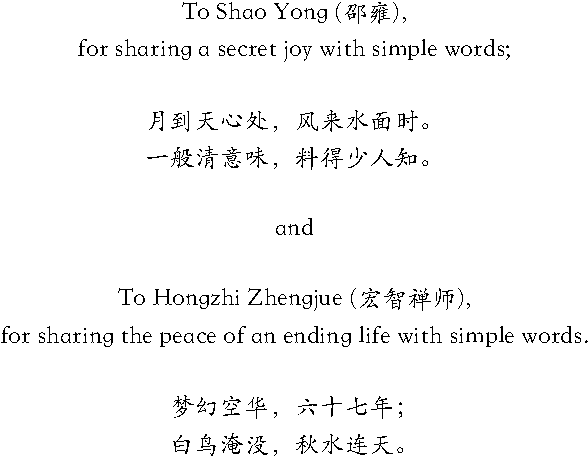
\includegraphics{images/dedication.pdf}
\end{center}

\setlength{\abovedisplayskip}{-5pt}
\setlength{\abovedisplayshortskip}{-5pt}

{
\hypersetup{linkcolor=black}
\setcounter{tocdepth}{1}
\tableofcontents
}
\listoftables
\listoffigures
\chapter{Introduction}\label{introduction}

This book is an early version of an ongoing project to equip students
with the basic knowledge to master ``statistical programming'' with R.

The statistical software \texttt{R} has come into prominence due to its
flexibility as an efficient language that builds a bridge between
software development and data analysis. For example, one strength of
\texttt{R} is the facility to develop and quickly adapt to the different
needs coming from the data management and analysis community while at
the same time making use of other languages in order to deliver
computationally efficient solutions. This book intends to present an
approachable framework to statistical programming and software
development using the wide variety of tools made available through
\texttt{R}, from method-specific packages to version control programs.
The general goals of the book are therefore the following:

\begin{itemize}
\tightlist
\item
  introduce tools and workflow for reproducible research (R/RStudio,
  Git/GitHub, etc.);
\item
  introduce principles of tidy data and tools for data wrangling;
\item
  exploit data structures to appropriately manage data, computer memory
  and computations;
\item
  data manipulation through controls, instructions, and tailored
  functions;
\item
  develop new software tools including functions, Shiny applications,
  and packages;
\item
  manage software development process including version control,
  documentation (with embedded code), and dissemination for other users.
\end{itemize}

The rest of this introductory chapter will present the R software by
explaining why it is used for this book and describing the basic
notations and tools that need to be known in order to better grasp its
contents.

\BeginKnitrBlock{rmdimportant}
This document is \textbf{under development} and it is therefore
preferable to always access the text online to be sure you are using the
most up-to-date version. Due to its current development, you may
encounter errors ranging from broken code to typos or poorly explained
topics. If you do, please let us know! Simply add an issue to the GitHub
repository used for this document (accessed here
\url{https://github.com/SMAC-Group/ds/issues}) and we will make the
changes as soon as possible. In addition, once you have learned
RMarkdown and GitHub, feel free to make a pull request to offer bug
fixes or corrections!
\EndKnitrBlock{rmdimportant}

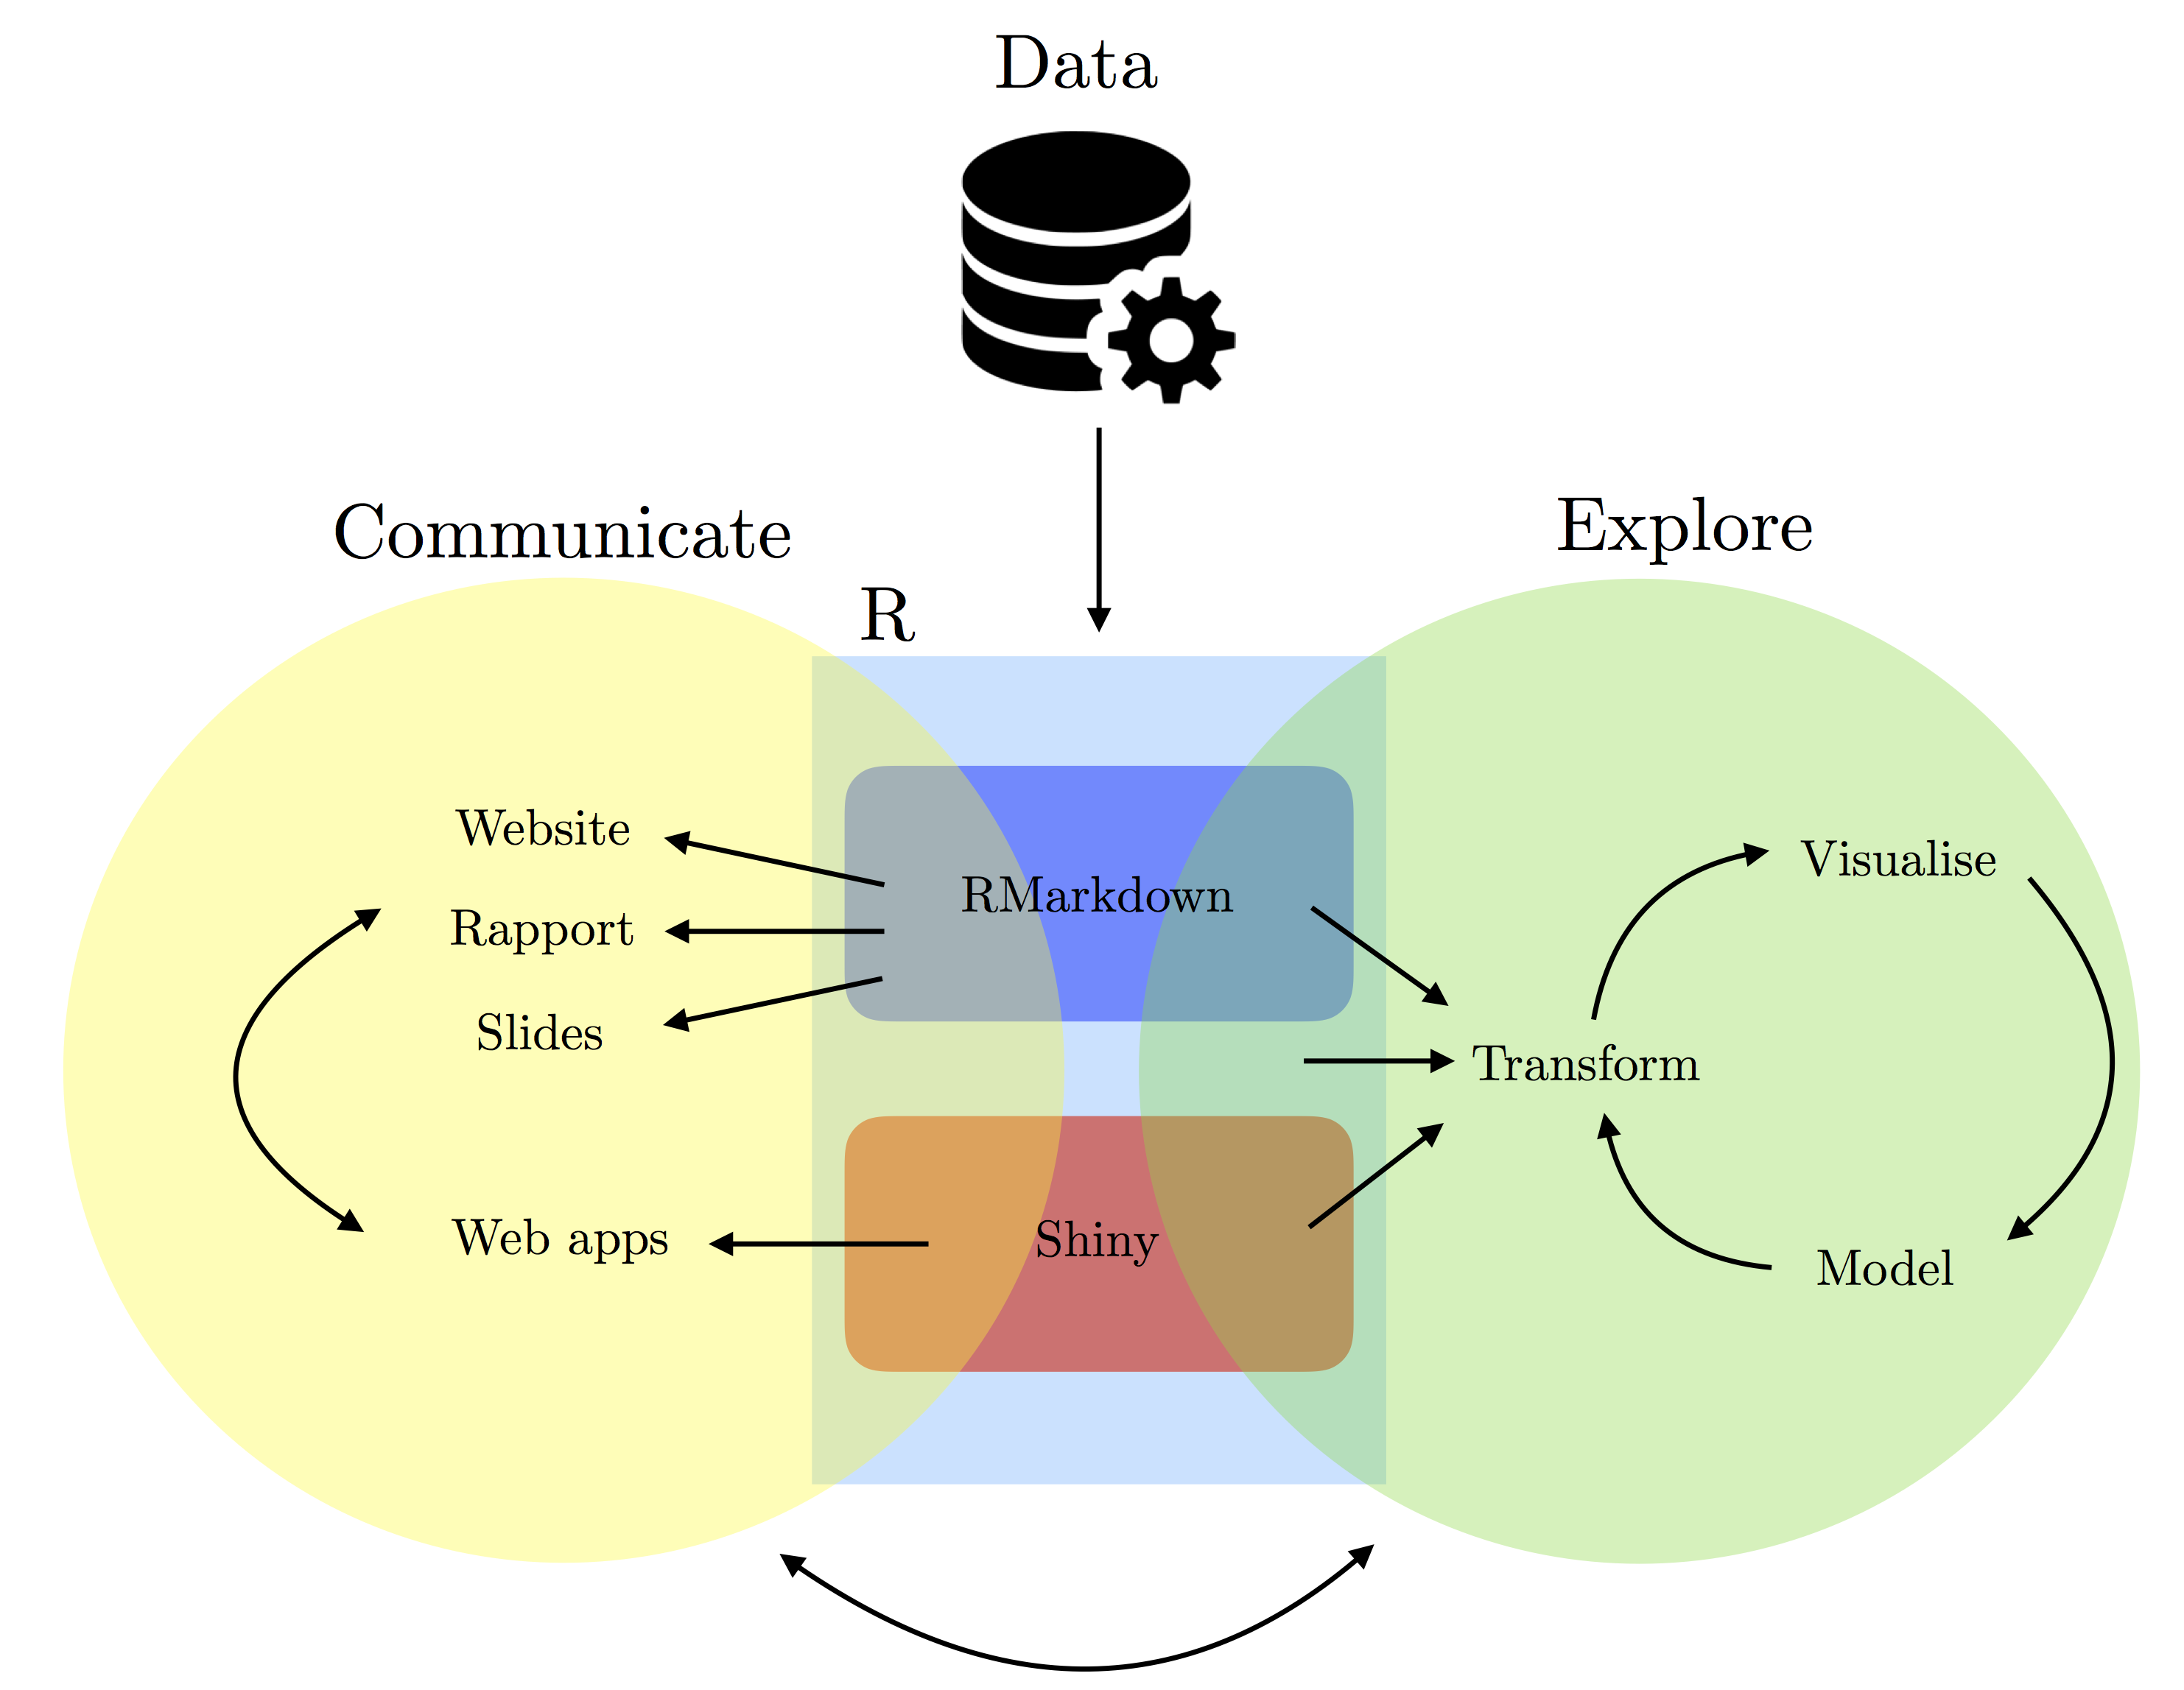
\includegraphics{images/diagram.png}

To demonstrate our goals, we will try to implement the process that is
mentioned in the diagram above. In many cases, an input (e.g.~data
source) is provided, and then we process, explore, and/or manipulate the
data with R. We then may communicate our findings through websites,
reports, slides, etc. using some combination of RMarkdown, R, and/or
Shiny. This process is not always sequential as we often have new ideas
or observations at any stage and begin exploring again.

\section{\texorpdfstring{\texttt{R} and
\texttt{RStudio}}{R and RStudio}}\label{r-and-rstudio}

The statistical computing language
\href{https://cran.r-project.org/}{\texttt{R}} has become commonplace
for many applications in industry, government, and academia. Having
started as an open-source language to make available different
statistics and analytical tools to researchers and the public, it
steadily developed into one of the major software languages which not
only allows to develop up-to-date, sound, and flexible analytical tools,
but also to include these tools within a framework which is
well-integrated with other important tools. The latter is amplified
thanks to the development of the
\href{https://www.rstudio.com/}{RStudio} interface which provides a
pleasant and functional user-interface for \texttt{R} as well as an
efficient Integrated Development Environment (IDE) in which different
programming languages, web-applications and other important tools are
readily available to the user. In order to illustrate the relationship
between R \& RStudio in statistical programming, one might think of a
car analogy in which R would be the drivetrain and chassis while RStudio
adds comfortable seats and air conditioning. R is doing most of the
work, and the user can basically get where they want to go using R
without RStudio. RStudio is generally is making you more comfortable
while you use R, but you won't get very far using RStudio without R.

\subsection{\texorpdfstring{Getting started with
\texttt{R}}{Getting started with R}}\label{getting-started-with-r}

Since \texttt{R} is a free and open-source software, you may simply
download it from the following link:

\begin{itemize}
\tightlist
\item
  \href{https://cran.r-project.org/}{\texttt{R}:
  https://cran.r-project.org/}
\end{itemize}

While \texttt{R} certainly can be used ``as is'' for many purposes, we
strongly recommend using an IDE called RStudio. There are several
versions of RStudio for different users (RStudio Desktop, Commercial,
Server, etc.). The free RStudio Desktop version is sufficient for our
purposes. RStudio can downloaded from the following link:

\begin{itemize}
\tightlist
\item
  \href{https://www.rstudio.com/}{RStudio: https://www.rstudio.com/}
\end{itemize}

\BeginKnitrBlock{rmdimportant}
You cannot use \texttt{RStudio} without having installed \texttt{R} on
your computer.
\EndKnitrBlock{rmdimportant}

\subsection{\texorpdfstring{Why \texttt{R}?}{Why R?}}\label{why-r}

There are many reasons to use \texttt{R}. Two compelling reasons are
that R is both free as in ``free pizza'', and free as in ``free
speech''. Free--like ``free pizza''--means that there is never a need to
pay for any part of the R software, or contributed packages (i.e.~add-on
modules). Free--like ``free speech''--means that there are very few
restrictions on how R can be used or barriers to those who would like to
contribute packages (i.e.~add-on modules).

The fact that is a free and open-source software does not necessarily
imply that it is a good software (although it is also that). The reason
why this is an important feature consists in the fact that the results
of any code or program developed in the \texttt{R} environment can
easily be replicated therefore ensuring accessibility and transparency
for the general user. More importantly however, this replicability of
results is also accompanied by a wide variety of packages that are made
available through the \texttt{R} environment in which users can find a
diversity of codes, functions, and features that are designed to tackle
a large amount of programming and analytical tasks. Moreover, new
packages are relatively simple to create and are extremely useful for
code-sharing purposes since they enclose the codes, functions, and
external dependencies that allow anyone to easily and efficiently
install these features. Additionally, these accessibility and
code-sharing features have established \texttt{R} as a platform for
development and dissemination of cutting-edge tools directly from the
developer to the end-user.

\subsection{About RStudio}\label{about-rstudio}

\texttt{RStudio} is a customizable IDE for the \texttt{R} enviornment
where the user can have easy access to plots, data, help, files, objects
and many other features that are useful to work efficiently with
\texttt{R}. For the most part, \texttt{RStudio} provides nearly
everything the \texttt{R} user will need in a self-contained, and
well-organized environment. Moreover, it is possible to create
``projects'' in which it is possible to create a dedicated environment
space for sets of specific functions and files aimed to deal with
various tasks.

Below is short video demonstrating a basic introduction of RStudio and
some of its elements.

In addition, \texttt{RStudio} provides embedded functionality to utilize
collaborative version-control software including GitHub \& Subversion as
well as a set of powerful tools to save and communicate results (whether
they be simulations, data analysis, or presenting and making available a
new package to other users). Some examples of these tools are
\texttt{Rmarkdown} which can be used respectively to integrate written
narrative with embedded \texttt{R} code and other content, as well as
and \texttt{Shiny\ Web\ Apps} which can provide an interactive
user-friendly interface that permits a user to actively engage with a
wide variety of tools built in \texttt{R} without the need to encounter
raw \texttt{R} code. GitHub and \texttt{Rmarkdown} will be the object of
a more in-depth description in the first chapters of this book in order
to provide the reader with the version-control and annotation tools that
can be useful for the following chapters of this book.

\subsection{Conventions}\label{conventions}

Throughout this book, \texttt{R} code will be typeset using a
\texttt{monospace} font which is syntax highlighted. For example:

\begin{Shaded}
\begin{Highlighting}[]
\NormalTok{a <-}\StringTok{ }\NormalTok{pi}
\NormalTok{b <-}\StringTok{ }\FloatTok{0.5}
\KeywordTok{sin}\NormalTok{(a}\OperatorTok{*}\NormalTok{b)}
\end{Highlighting}
\end{Shaded}

Similarly, \texttt{R} output lines (that usally appear in your Console)
will begin with \texttt{\#\#} and will not be syntax highlighted. The
output of the above example is the following:

\begin{verbatim}
## [1] 1
\end{verbatim}

Aside from \texttt{R} code and output, this book will also insert boxes
in order to draw the reader's attention to important, curious, or
otherwise informative details. An example of these boxes was seen at the
beginning of this introduction where an important aspect was pointed out
to the reader regarding the ``under construction'' nature of this book.
Therefore the following boxes and symbols can be used to represent
information of different nature:

\BeginKnitrBlock{rmdnote}
This is a \textbf{note} that could be interesting or useful to the
reader.
\EndKnitrBlock{rmdnote}

\BeginKnitrBlock{rmdtip}
This is a \textbf{tip} for implementing content from this book.
\EndKnitrBlock{rmdtip}

\BeginKnitrBlock{rmdimportant}
This highlights \textbf{important information}.
\EndKnitrBlock{rmdimportant}

\BeginKnitrBlock{rmdcaution}
This is a \textbf{caution} to help the reader avoid minor problems.
\EndKnitrBlock{rmdcaution}

\BeginKnitrBlock{rmdwarning}
This is a \textbf{warning} to help the reader avoid significant
problems.
\EndKnitrBlock{rmdwarning}

\subsection{Getting help}\label{getting-help}

In the previous section we presented some examples on how \texttt{R} can
be used as a calculator and we have already seen several functions such
as \texttt{sqrt()} or \texttt{log()}. To obtain documentation about a
function in \texttt{R}, simply put a question mark in front of the
function name (or just type \texttt{help()} around the function name),
or use the search bar on the ``Help'' tab in your RStudio window, and
its documentation will be displayed. For example, if you are interested
in learning about the function \texttt{log()} you could simply type:

\begin{Shaded}
\begin{Highlighting}[]
\NormalTok{?log}
\end{Highlighting}
\end{Shaded}

which will display something similar to:

\begin{figure}
\centering
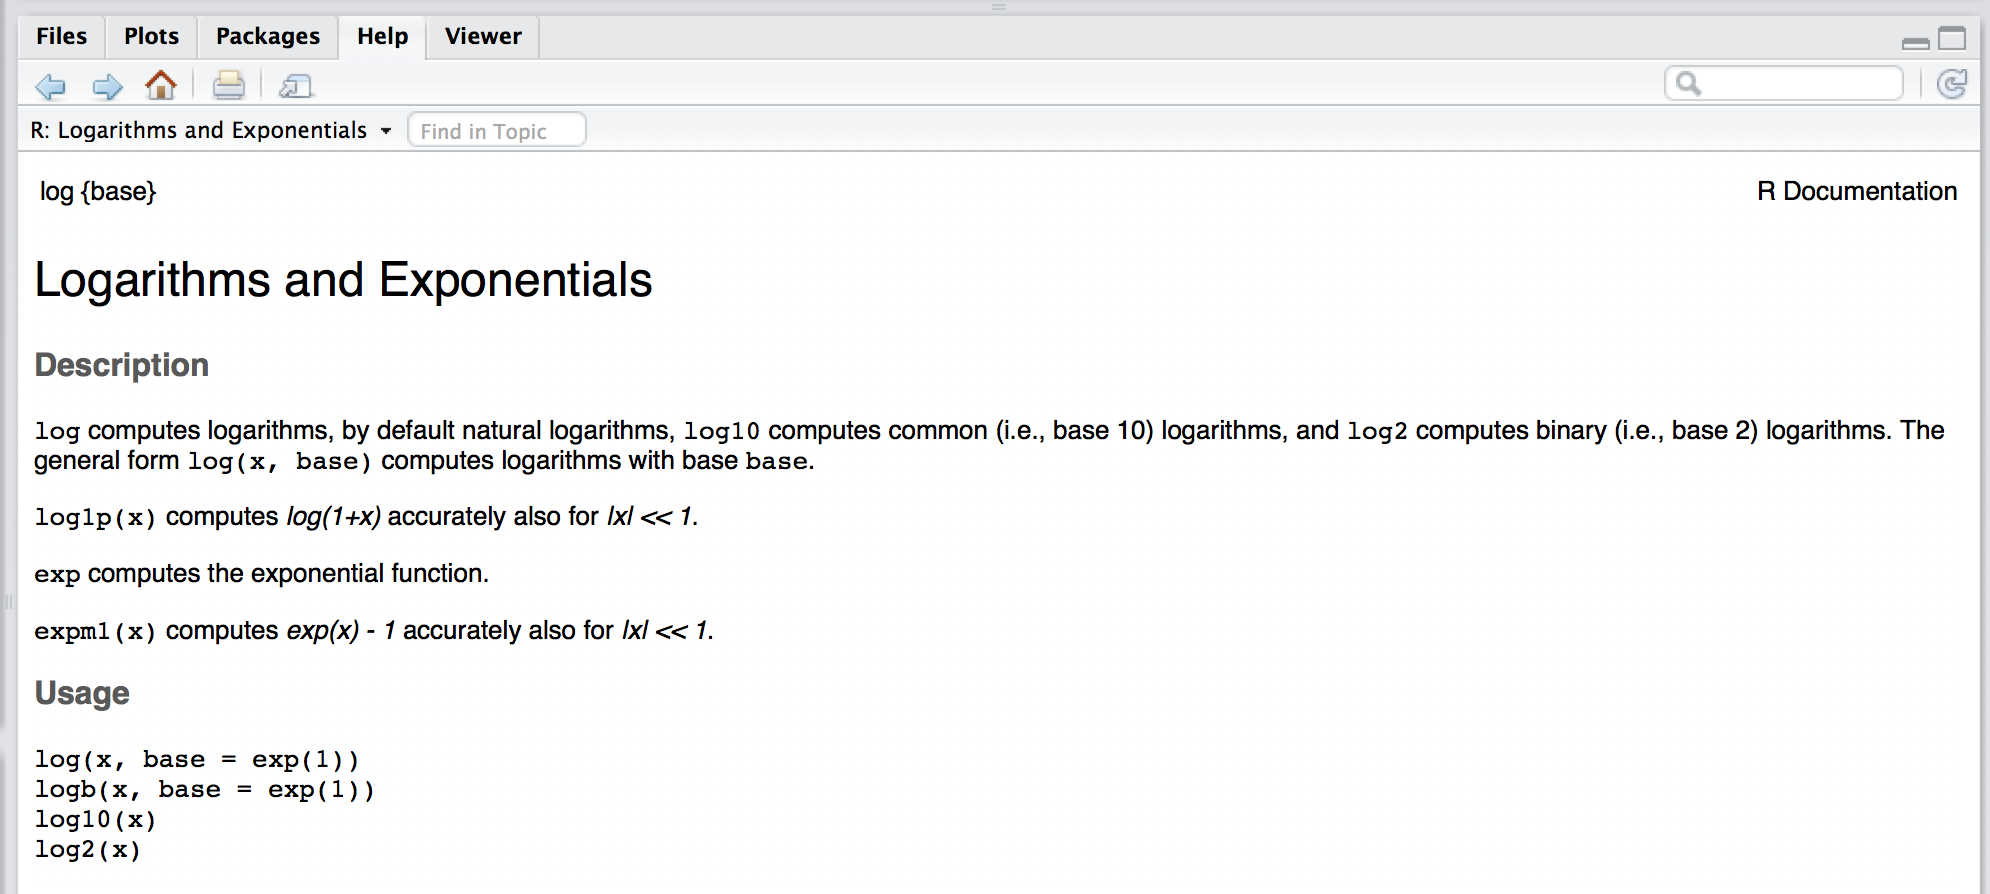
\includegraphics{images/example-log-help.png}
\caption{}
\end{figure}

The \texttt{R} documentation is written by the author of the package.
For mainstream packages in widespread use, the documentation is almost
always quite good, but in some cases it can be quite technical,
difficult to interpret, and possibly incomplete. In these cases, the
best solution to understand a function is to search for help on any
search engine. Often a simple search like ``side by side boxplots in R''
or ``side by side boxplots in ggplot2'' will produce many useful
results. The search results often include user forums such as
``CrossValidated'' or ``StackExchange'' in which the questions you have
about a function have probably already been asked and answered by many
other users.

\BeginKnitrBlock{rmdtip}
You can often use the error message to search for answers about a
problem you may have with a function.
\EndKnitrBlock{rmdtip}

\subsection{Installing packages}\label{installing-packages}

\texttt{R} comes with a number of built-in functions but one of its main
strengths is that there is a large number of packages on an
ever-increasing range of subjects available for you to install. These
packages provide additional functions, features and data to the R
environement. If you want to do something in \texttt{R} that is not
available by default, there is a good chance that there are packages
that will respond to your needs. In this case, an appropriate way to
find a package in \texttt{R} is to use the search option in the CRAN
repository which is the official network of file-transfer protocols and
web-servers that store updated versions of code and documentation for
\texttt{R} (see CRAN website). Another general approach to find a
package in \texttt{R} is simply to use a search engine in which to type
the keywords of the tools you are looking for followed by ``R package''.

\texttt{R} packages can be installed in various ways but the most widely
used approach is through the \texttt{install.packages()} function.
Another way is to use the ``Tools -\textgreater{} Install
Packages\ldots{}'' path from the dropdown menus in \texttt{RStudio} or
clicking on the ``install'' button in the ``Packages'' pane in the
RStudio environment. The \texttt{install.packages()} function is very
straight-forward and transcends any platform for the \texttt{R}
environment. It is noteworthy that this approach assumes that the
desired package(s) are available within the CRAN repository. This is
very often the case, but there is a growing number of packages that are
under-development or completed and are made available through other
repositories. In the latter setting, Chapter 02 will show other ways of
installing packages from a commonly used repository called ``GitHub''.

Sticking momentarily to the packages available in the CRAN repository,
the use of the \texttt{install.packages()} is quite simple. For example,
if you want to install the package \texttt{devtools} you can simply
write:

\begin{Shaded}
\begin{Highlighting}[]
\KeywordTok{install.packages}\NormalTok{(}\StringTok{"devtools"}\NormalTok{)}
\end{Highlighting}
\end{Shaded}

Once a package is installed it is not directly usable within your
\texttt{R} session. To do so you will have to ``load'' the package into
your current \texttt{R} session which is generally done through the
function \texttt{library()}. For example, after having installed the
\texttt{devtools} package, in order to use it within your session you
would write:

\begin{Shaded}
\begin{Highlighting}[]
\KeywordTok{library}\NormalTok{(devtools)}
\end{Highlighting}
\end{Shaded}

Once this is done, all the functions and documentation of this package
are available and can be used within your current session. However, once
you close your \texttt{R} session, all loaded packages will be closed
and you will have to load them again if you want to use them in a new
\texttt{R} session.

\BeginKnitrBlock{rmdnote}
Please notice that although packages need to be loaded at each session
if you want to use them, they need to be installed only once. The only
exception to this rule is when you need to update the package or
reinstall it for some reason.
\EndKnitrBlock{rmdnote}

One of the main packages that is required for this class would be our
STAT 297 package, that contains all the necessary packages and functions
that will be utilized in this book. Run the following code to install
the package directly from GitHub.

\begin{Shaded}
\begin{Highlighting}[]
\KeywordTok{install_github}\NormalTok{(}\StringTok{"SMAC-Group/stat297"}\NormalTok{)}
\end{Highlighting}
\end{Shaded}

\BeginKnitrBlock{rmdwarning}
The STAT 297 package is required for use of many features in this book.
\EndKnitrBlock{rmdwarning}

\subsection{Additional References}\label{additional-references}

There are many more elements in RStudio, and we encourage you to use the
\href{https://www.rstudio.com/wp-content/uploads/2016/01/rstudio-IDE-cheatsheet.pdf}{RStudio
Cheatsheet} as a reference.

\section{\texorpdfstring{Basic Probability and Statistics with
\texttt{R}}{Basic Probability and Statistics with R}}\label{basic-probability-and-statistics-with-r}

The \texttt{R} environment provides an up-to-date and efficient
programming language to develop different tools and applications.
Nevertheless, its main functionality lies in the core statistical
framework and tools that consistute the basis of this language. Indeed,
this book aims at introducing and describing the methods and approaches
of statistical programming which therefore require a basic knowledge of
Probability and Statistics in order to grasp the logic and usefulness of
the features presented in this book.

For this reason, we will briefly take the reader through some of the
basic functions that are available within \texttt{R} to obtain
probabilities based on parametric distributions, compute summary
statistics and understand basic data structures. The latter is just an
introduction and a more in-depth description of different data
structures will be given in a future chapter.

\subsection{Simple calculations}\label{simple-calculations}

Since the \texttt{R} environment can serve as an advanced calculator, it
is worth noting this also allows for simple calculations. In the table
below we show a few examples of such calculations where the first column
gives a mathematical expression (calculation), the second gives the
equivalent of this expression in \texttt{R} and finally in the third
column we can find the result that is output from \texttt{R}.

\begin{longtable}[]{@{}lll@{}}
\toprule
Math. & R & Result\tabularnewline
\midrule
\endhead
2+2 & \texttt{2+2} & \texttt{4}\tabularnewline
\(\frac{4}{2}\) & \texttt{4/2} & \texttt{2}\tabularnewline
\(3 \cdot 2^{-0.8}\) & \texttt{3*2\^{}(-0.8)} &
\texttt{1.723048}\tabularnewline
\(\sqrt{2}\) & \texttt{sqrt(2)} & \texttt{1.414214}\tabularnewline
\(\pi\) & \texttt{pi} & \texttt{3.141593}\tabularnewline
\(\ln(2)\) & \texttt{log(2)} & \texttt{0.6931472}\tabularnewline
\(\log_{3}(9)\) & \texttt{log(9,\ base\ =\ 3)} &
\texttt{2}\tabularnewline
\(e^{1.1}\) & \texttt{exp(1.1)} & \texttt{3.004166}\tabularnewline
\(\cos(\sqrt{0.9})\) & \texttt{cos(sqrt(0.9))} &
\texttt{0.5827536}\tabularnewline
\bottomrule
\end{longtable}

\subsection{Probability Distributions}\label{probability-distributions}

Probability distributions can be uniquely characterized by different
functions such as, for example, their density or distribution functions.
Based on these it is possible to compute theoretical quantiles and also
randomly sample observations from them. Replacing the \texttt{R} syntax
for a given probability distribution with the general syntax
\texttt{name}, all these functions and calculations are made available
in \texttt{R} through the built-in functions:

\begin{itemize}
\tightlist
\item
  \texttt{dname} calculates the value of the density function (pdf);
\item
  \texttt{pname} calculates the value of the distribution function
  (cdf);
\item
  \texttt{qname} calculates the value of the theoretical quantile;
\item
  \texttt{rname} generates a random sample from a particular
  distribution.
\end{itemize}

Note that, when using these functions in practice, \texttt{name} is
replaced with the syntax used in \texttt{R} to denote a specific
probability distribution. For example, if we wish to deal with a Uniform
probability distribution, then the syntax \texttt{name} is replaced by
\texttt{unif} and, furthering the example, to randomly generate
observations from a uniform distribution the function to use will be
therefore \texttt{runif}. \texttt{R} allows to make use of these
functions for a wide variety of probability distributions that include,
but are not limited to: Gaussian (or Normal), Binomial, Chi-square,
Exponential, F-distribution, Geometric, Poisson, Student-t and Uniform.
In order to get an idea of how these functions can be used, below is an
example of a problem that can be solved using them.

\subsubsection{Example: Normal Test Scores of College Entrance
Exam}\label{example-normal-test-scores-of-college-entrance-exam}

Assume that the test scores of a college entrance exam follows a Normal
distribution. Furthermore, suppose that the mean test score is 70 and
that the standard deviation is 15. How would we find the percentage of
students scoring 90 or more in this exam?

In this case, we consider a random variable \(X\) that is normally
distributed as follows: \(X \sim N(\mu=70, \sigma^2=225)\) where \(\mu\)
and \(\sigma^2\) represent the mean and variance of the distribution
respectively. Since we are looking for the probability of students
scoring higher than 90, we are interested in finding
\(\mathbb{P}(X > x=90)\) and therefore we look at the upper tail of the
Normal distribution. To find this probability we need the distribution
function (\texttt{pname}) for which we therefore replace \texttt{name}
with the \texttt{R} syntax for the Normal distribution: \texttt{norm}.
The distribution function in \texttt{R} has various parameters to be
specified in order to compute a probability which, at least for the
Normal distribution, can be found by typing \texttt{?pnorm} in the
Console and are:

\begin{itemize}
\tightlist
\item
  \texttt{q}: the quantile we are interested in (e.g.~90);
\item
  \texttt{mean}: the mean of the distribution (e.g.~70);
\item
  \texttt{sd}: the standard deviation of the distribution (e.g.~15);
\item
  \texttt{lower.tail}: a boolean determining whether to compute the
  probability of being smaller than the given quantile (i.e.
  \(\mathbb{P}(X \leq x)\)) which requires the default argument
  \texttt{TRUE} or larger (i.e. \(\mathbb{P}(X > x)\)) which requires to
  specify the argument \texttt{FALSE}.
\end{itemize}

Knowing these arguments, it is now possible to compute the probability
we are interested in as follows:

\begin{Shaded}
\begin{Highlighting}[]
\KeywordTok{pnorm}\NormalTok{(}\DataTypeTok{q =} \DecValTok{90}\NormalTok{, }\DataTypeTok{mean =} \DecValTok{70}\NormalTok{, }\DataTypeTok{sd =} \DecValTok{15}\NormalTok{, }\DataTypeTok{lower.tail =} \OtherTok{FALSE}\NormalTok{) }
\end{Highlighting}
\end{Shaded}

\begin{verbatim}
## [1] 0.09121122
\end{verbatim}

As we can see from the output, there is roughly a 9\% probability of
students scoring 90 or more on the exam.

\subsection{Summary Statistics}\label{summary-statistics}

While the previous functions deal with theoretical distributions, it is
also necessary to deal with real data from which we would like to
extract information. Supposing--as is often the case in applied
statistics--we don't know from which distribution it is generated, we
would be interested in understanding the behavior of the data in order
to eventually identify a distribution and estimate its parameters.

The use of certain functions varies according to the nature of the
inputs since these can be, for example, numerical or factors.

\subsubsection{Numerical Input}\label{numerical-input}

A first step in analysing numerical inputs is given by computing summary
statistics of the data which, in this section, we can generally denote
as \texttt{x} (we will discuss the structure of this data more in detail
in the following chapters). For central tendency or spread statistics of
a numerical input, we can use the following \texttt{R} built-in
functions:

\begin{itemize}
\tightlist
\item
  \texttt{mean} calculates the mean of an input \texttt{x};
\item
  \texttt{median} calculates the median of an input \texttt{x};
\item
  \texttt{var} calculates the variance of an input \texttt{x};
\item
  \texttt{sd} calculates the standard deviation of an input \texttt{x};
\item
  \texttt{IQR} calculates the interquartile range of an input
  \texttt{x};
\item
  \texttt{min} calculates the minimum value of an input \texttt{x};
\item
  \texttt{max} calculates the maximum value of an input \texttt{x};
\item
  \texttt{range} returns a vector containing the minimum and maximum of
  all given arguments;
\item
  \texttt{summary} returns a vector containing a mixture of the above
  functions (i.e.~mean, median, first and third quartile, minimum,
  maximum).
\end{itemize}

\subsubsection{Factor Input}\label{factor-input}

If the data of interest is a factor with different categories or levels,
then different summaries are more appropriate. For example, for a factor
input we can extract counts and percentages to summarize the variable by
using \texttt{table}. Using functions and data structures that will be
described in the following chapters, below we create an example dataset
with 90 observations of three different colors: 20 being
\texttt{Yellow}, 10 being \texttt{Green} and 50 being \texttt{Blue}. We
then apply the \texttt{table} function to it:

\begin{Shaded}
\begin{Highlighting}[]
\KeywordTok{table}\NormalTok{(}\KeywordTok{as.factor}\NormalTok{(}\KeywordTok{c}\NormalTok{(}\KeywordTok{rep}\NormalTok{(}\StringTok{"Yellow"}\NormalTok{, }\DecValTok{20}\NormalTok{), }\KeywordTok{rep}\NormalTok{(}\StringTok{"Green"}\NormalTok{, }\DecValTok{10}\NormalTok{), }\KeywordTok{rep}\NormalTok{(}\StringTok{"Blue"}\NormalTok{, }\DecValTok{50}\NormalTok{))))}
\end{Highlighting}
\end{Shaded}

\begin{verbatim}
## 
##   Blue  Green Yellow 
##     50     10     20
\end{verbatim}

By doing so we obtain a frequency (count) table of the colors.

\subsubsection{Dataset Inputs}\label{dataset-inputs}

In many cases, when dealing with data we are actually dealing with
datasets (see Chapter 03) where variables of different nature are
aligned together (usually in columns). For datasets there is another
convenient way to get simple summary statistics which consists in
applying the function \texttt{summary} to the dataset itself (instead of
simply a numerical input as seen earlier).

As an example, let us explore the
\href{https://en.wikipedia.org/wiki/Iris_flower_data_set}{Iris} flower
dataset contained in the \texttt{R} built-in \texttt{datasets} package.
The data set consists of 50 samples from each of three species of Iris
(Setosa, Virginica and Versicolor). Four features were measured from
each sample consisting in the length and the width (in centimeters) of
the both sepals and petals. This dataset is widely used as an example
since it was used by Fisher to develop a linear discriminant model based
on which he intended to distinguish the three species from each other
using combinations of these four features.

Using this dataset, let us use the \texttt{summary} function on it to
output the minimum, first quartile and thrid quartile, median, mean and
maximum statistics (for the numerical variables in the dataset) and
frequency counts (for factor inputs).

\begin{Shaded}
\begin{Highlighting}[]
\KeywordTok{summary}\NormalTok{(iris)}
\end{Highlighting}
\end{Shaded}

\begin{verbatim}
##   Sepal.Length    Sepal.Width     Petal.Length    Petal.Width   
##  Min.   :4.300   Min.   :2.000   Min.   :1.000   Min.   :0.100  
##  1st Qu.:5.100   1st Qu.:2.800   1st Qu.:1.600   1st Qu.:0.300  
##  Median :5.800   Median :3.000   Median :4.350   Median :1.300  
##  Mean   :5.843   Mean   :3.057   Mean   :3.758   Mean   :1.199  
##  3rd Qu.:6.400   3rd Qu.:3.300   3rd Qu.:5.100   3rd Qu.:1.800  
##  Max.   :7.900   Max.   :4.400   Max.   :6.900   Max.   :2.500  
##        Species  
##  setosa    :50  
##  versicolor:50  
##  virginica :50  
##                 
##                 
## 
\end{verbatim}

\section{Main References}\label{main-references}

This is not the first (or the last) book that has been written
explaining and describing statistical programming in \texttt{R}. Indeed,
this can be seen as a book that brings together and reorganizes
information and material from other sources structuring and tailoring it
to a course in basic statistical programming. The main references (which
are far from being an exhaustive review of literature) that can be used
to have a more in-depth view of different aspects treated in this book
are:

\begin{itemize}
\tightlist
\item
  \citet{wickham2014advanced} : a more technical and advanced
  introduction to \texttt{R};
\item
  \citet{wickham2015packages} : basic building blocks of building
  packages in \texttt{R};
\item
  \citet{xie2015} : an overview of document generation in \texttt{R};
\end{itemize}

\section{License}\label{license}

You can redistribute it and/or modify this book under the terms of the
Creative Commons Attribution-NonCommercial-ShareAlike 4.0 International
License (CC BY-NC-SA) 4.0 License.

\part{Foundation}\label{part-foundation}

\chapter{RMarkdown}\label{rmarkdown}

RMarkdown is a framework that provides a literate programming format for
data science. It can be used to save and execute R code within RStudio
and also as a simple formatting syntax for authoring HTML, PDF, ODT,
RTF, and MS Word documents as well as seamless transitions between
available formats. The name ``markdown'' is an intentional contrast to
other ``markup'' languages--e.g., hypertext markup language
(HTML)--which require syntax that can be quite difficult to decipher for
the uninitiated. One aim of the markdown paradigm is a syntax that is as
human-readable as possible. ``RMarkdown'' is an implementation of the
``markdown'' language designed to accommodate embedded \texttt{R} code.

\subsection*{\texorpdfstring{What is \textbf{literate}
programming?}{What is literate programming?}}\label{what-is-literate-programming}

Literate programming is the notion for programmers of adding narrative
context with code to produce documentation for the program
simultaneously. Consequently, it is possible to read through the code
with explanations so that any viewer can follow through the
presentation. RMarkdown offers a simple tool that allows to create
reports or presentation slides in a reproducible manner with collateral
advantages such as avoiding repetitive tasks by, for example, changing
all figures when data are updated.

\subsection*{\texorpdfstring{What is \textbf{reproducible}
research?}{What is reproducible research?}}\label{what-is-reproducible-research}


Reproducible research or reproducible analysis is the notion that an
experiment's whole process, including collecting data, performing
analysis and producing output, can be reproduced the same way by someone
else. Building non-reproducible experiments has been a problem both in
research and in the industry, and having such an issue highly decreases
the credibility of the authors' findings and, potentially, the authors
themselves. In essence, allowing for reproducible research implies that
anyone could run the code (knit the document, etc.) and obtain the same
exact results as the original research and RMarkdown is commonly used to
address this issue.

Below is a short video showing a basic overview of RMarkdown.

Below, we have created a framework application that you can use to test
out different RMarkdown functions. Experiment with different R Markdown
elements and utilize it to practice building and knitting HTML output.

You can access the online versions here:

\begin{itemize}
\tightlist
\item
  \href{http://shiny.science.psu.edu/szg279/rmd/}{RMarkdown Web}
\item
  \href{http://shiny.science.psu.edu/szg279/rmd_mini/}{RMarkdown Mobile}
\end{itemize}

or simply run it within the \texttt{stat297} package by using either

\begin{Shaded}
\begin{Highlighting}[]
\CommentTok{# RMarkdown Web}
\NormalTok{stat297}\OperatorTok{::}\KeywordTok{runShiny}\NormalTok{(}\StringTok{'rmd'}\NormalTok{)}

\CommentTok{# RMarkdown Mobile}
\NormalTok{stat297}\OperatorTok{::}\KeywordTok{runShiny}\NormalTok{(}\StringTok{'rmd_mini'}\NormalTok{)}
\end{Highlighting}
\end{Shaded}

\section{Create an R Markdown file in
RStudio}\label{create-an-r-markdown-file-in-rstudio}

Within RStudio, click \texttt{File} → \texttt{New\ File} →
\texttt{R\ Markdown}. Give the file a title and the author (your name)
and select the default output, HTML. We can change this later so don't
worry about it for the moment.

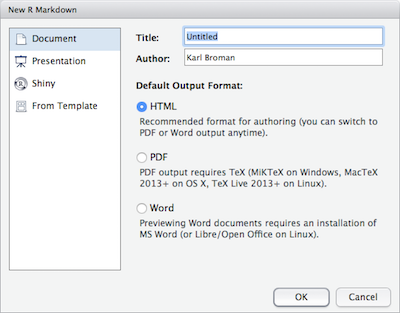
\includegraphics{images/rmd_new.png}

An RMarkdown is a plain text file that contains three different aspects:

\begin{itemize}
\tightlist
\item
  YAML metadata
\item
  Text
\item
  Code Chunks
\end{itemize}

\section{YAML Metadata}\label{yaml-metadata}

YAML stands for \emph{YAML Ain't Markup Language} and is used to specify
document configurations and properties such as name, date, output
format, etc. The (optional) YAML header is surrounded before and after
by ``---'' on a dedicated line.

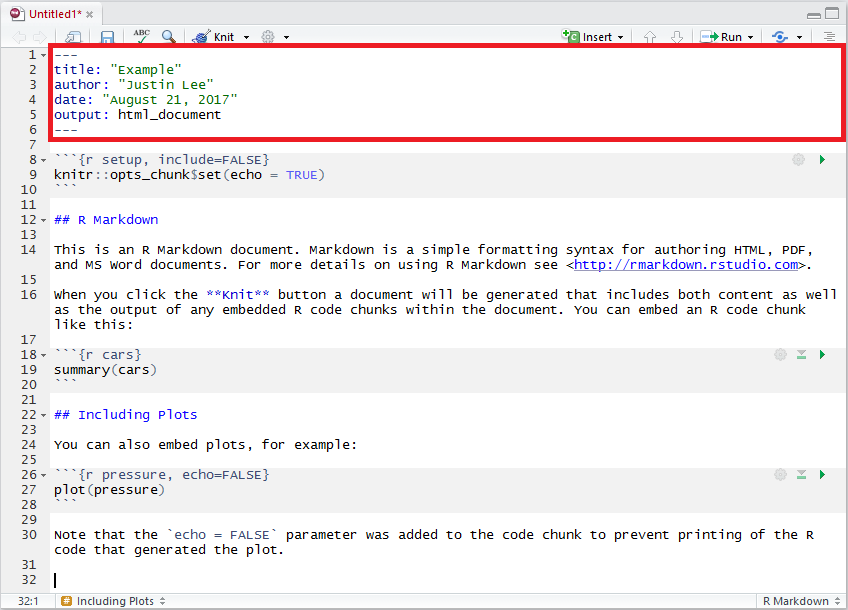
\includegraphics{images/rmd_yaml.png}

You can also include additional formatting
\href{http://RMarkdown.rstudio.com/html_document_format.html}{options}
such as a table of contents or even a custom CSS style template which
can be used to further enhance the presentation. For the purpose of this
book, the default options should be sufficient. Below is an example knit
output of the above RMarkdown file.

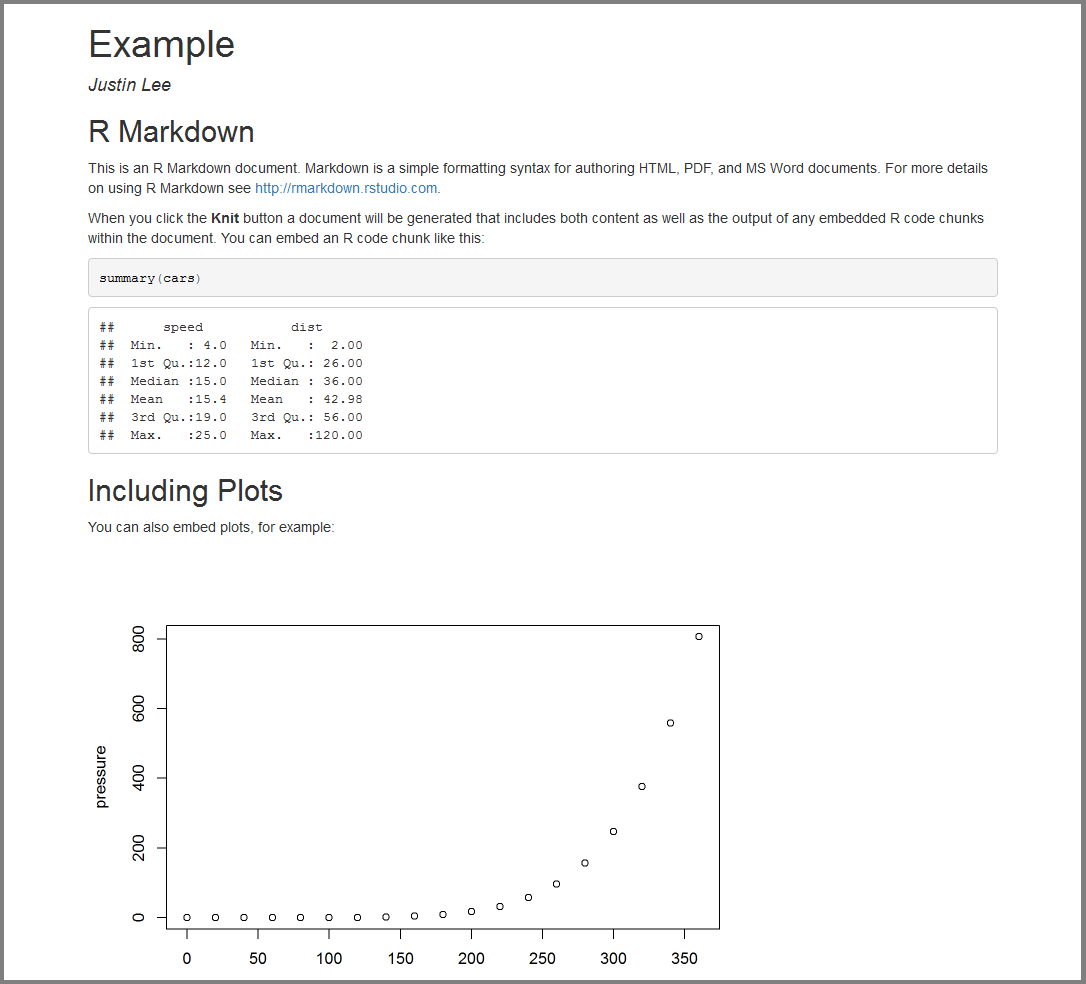
\includegraphics{images/rmd_example_output.png}

The default output above is an html\_document format but this format can
be modified using, for example, \texttt{pdf\_document} to output a pdf.
However, the pdf format requires additional installation and
configuration of a TeX distribution such as
\href{https://miktex.org/2.9/setup}{MikTeX}. Once available, the user
can also include raw LaTeX and even define LaTeX macros in the RMarkdown
document if necessary (we'll discuss more about LaTeX further on).

\subsection{Subsections}\label{subsections}

To make your sections numbered as sections and subsections, make sure
you specify \texttt{number\_sections:\ yes} as part of the YAML Metadata
as shown below.

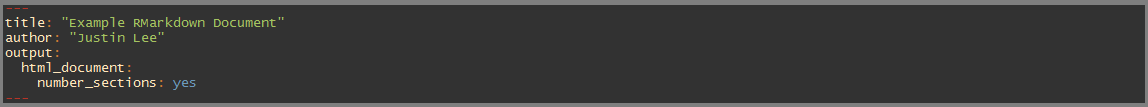
\includegraphics{images/yaml_number_sections.png}

\section{Text}\label{text}

Due to its literate nature, text will be an essential part in explaining
your analysis. With RMarkdown, we can specify custom text formatting
with emphases such as \emph{italics}, \textbf{bold}, or
\texttt{code\ style}. To understand how to format text, our previous
sentence would be typed out as follows in RMarkdown:

\begin{verbatim}
With RMarkdown, we can specify custom text formatting with emphases such as *italics*, **bold**, or `code style
\end{verbatim}

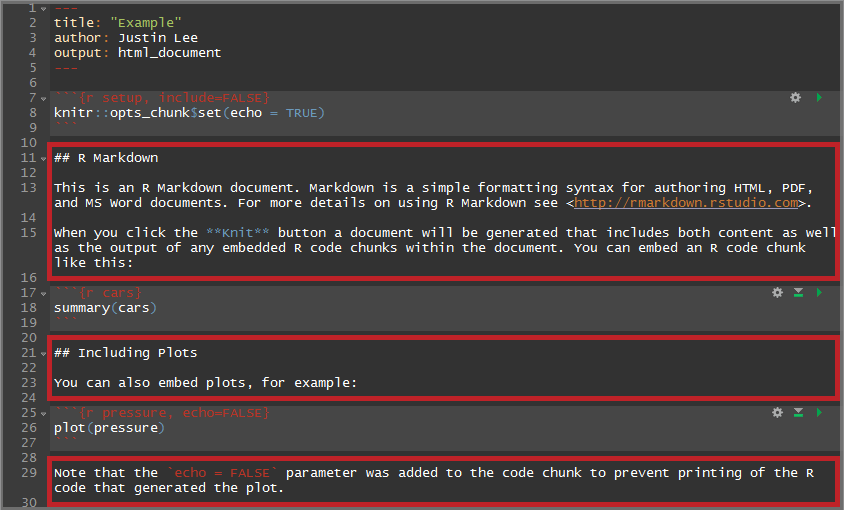
\includegraphics{images/rmd_text.png}

\subsection{Headers}\label{headers}

As seen above, headers are preceded by a \#. A single \texttt{\#}
produces the largest heading text while, to produce smaller headings,
you simply need to add more \texttt{\#}s! Heading level also impacts
section and subsection nesting in documents and tables of contents, as
well as slide breaks in presentation formats.

\subsection{Lists}\label{lists}

Lists can be extremely convenient to make text more readable or to take
course notes during class. RMarkdown allows to create different list
structures as shown in the code below:

\begin{verbatim}
* You can create bullet points by using symbols such as *, +, or -. 
+ simply add an indent or four preceding spaces to indent a list. 
    + You can manipulate the number of spaces or indents to your liking. 
        - Like this. 
    * Here we go back to the first indent. 
1. To make the list ordered, use numbers. 
1. We can use one again to continue our ordered list. 
2. Or we can add the next consecutive number. 
\end{verbatim}

which delivers the following list structure:

\begin{itemize}
\tightlist
\item
  You can create bullet points by using symbols such as *, +, or -.
\item
  simply add an indent or four preceding spaces to indent a list.

  \begin{itemize}
  \tightlist
  \item
    You can manipulate the number of spaces or indents to your liking.

    \begin{itemize}
    \tightlist
    \item
      Like this.
    \end{itemize}
  \item
    Here we go back to the first indent.
  \end{itemize}
\end{itemize}

\begin{enumerate}
\def\labelenumi{\arabic{enumi}.}
\tightlist
\item
  To make the list ordered, use numbers.
\item
  We can use one again to continue our ordered list.
\item
  Or we can add the next consecutive number.
\end{enumerate}

\subsection{Hyperlinks}\label{hyperlinks}

To add hyperlinks with the full link, (ex: \url{https://google.com/})
you can follow the syntax below:

\begin{verbatim}
<https://google.com/>
\end{verbatim}

whereas to add hyperlinks with a custom link title, (ex:
\href{https://google.com}{Google}) follow the syntax below:

\begin{verbatim}
[Google](https://google.com)
\end{verbatim}

\subsection{Blockquotes}\label{blockquotes}

Use the \textgreater{} character in front of a line, \emph{just like in
email} to produce blockquotes which styles the text in a way to use if
we quote a person, a song or another entity.

\begin{quote}
``To grow taller, you should shave your head. Remember to bring the
towels!''

Justin Lee
\end{quote}

\subsection{Pictures}\label{pictures}

To add a picture with captions, follow the syntax below:

\begin{verbatim}
![Eberly College of Science Banner](http://science.psu.edu/psu_eberly_blue.png)
\end{verbatim}

which will produce:


\includegraphics{http://science.psu.edu/psu_eberly_blue.png}

Otherwise, to add a picture without any captions, follow the syntax
below:

\begin{verbatim}
![](http://www.alumni.psu.edu/s/1218/16/images/logo.png)
\end{verbatim}

which delivers:


\includegraphics[width=0.50000\textwidth]{http://www.alumni.psu.edu/s/1218/16/images/logo.png}

\subsection{LaTeX}\label{latex}

LaTeX is a document preparation system that uses plain text as opposed
to formatted text that is used for applications such as Microsoft Word.
It is widely used in academia as a standard for the publication of
scientific documents. It has control over large documents containing
sectioning, cross-references, tables and figures.

\subsubsection{LaTeX in RMarkdown}\label{latex-in-rmarkdown}

Unlike a highly formatted word processor, we cannot produce equations by
clicking on symbols. As data scientists there is often the need to
explain distributions and equations that are behind the methods we
present. Within the text section of an RMarkdown document you can
include LaTeX format text to output different forms of text, mainly
equations and mathematical expressions.

Inline mathematical expressions can be added using the syntax:
\texttt{\$math\ expression\$}. For example, if we want to write ``where
\(\alpha\) is in degrees'' we would write:

\begin{verbatim}
"where $\alpha$ is in degrees".
\end{verbatim}

Using a slightly different syntax (i.e.
\texttt{\$\$math\ expression\$\$}) we can obtain centered mathematical
expressions. For example, the binomial probability distribution in LaTeX
is written as

\texttt{\$\$f(y\textbar{}N,p)\ =\ \textbackslash{}frac\{N!\}\{y!(N-y)!\}\textbackslash{}cdot\ p\^{}y\ \textbackslash{}cdot\ (1-p)\^{}\{N-y\}\ =\ \{\{N\}\textbackslash{}choose\{y\}\}\ \textbackslash{}cdot\ p\^{}y\ \textbackslash{}cdot\ (1-p)\^{}\{N-y\}\$\$}

which is output as:

\[f(y|N,p) = \frac{N!}{y!(N-y)!}\cdot p^y \cdot (1-p)^{N-y} = {{N}\choose{y}} \cdot p^y \cdot (1-p)^{N-y}\]

An introduction to the LaTeX format can be found
\href{http://www.math.harvard.edu/texman/}{here} if you want to learn
more about the basics. An alternative can be to insert custom LaTeX
formulas using a graphical interface such as
\href{https://www.codecogs.com/latex/eqneditor.php}{codecogs}.

\subsection{Cross-referencing
Sections}\label{cross-referencing-sections}

You can also use the same syntax \texttt{\textbackslash{}@ref(label)} to
reference sections, where label is the section identifier (ID). By
default, Pandoc will generate IDs for all section headers, e.g.,
\texttt{\#\ Hello\ World} will have an ID \texttt{hello-world}. To call
header \texttt{hello-world} as a header, we type
\texttt{\textbackslash{}@ref(hello-world)} to cross-reference the
section. In order to avoid forgetting to update the reference label
after you change the section header, you may also manually assign an ID
to a section header by appending \{\#id\} to it.

\subsection{Citations and
Bibliography}\label{citations-and-bibliography}

Citations and bibliographies can automatically be generated with
RMarkdown. In order to use this feature we first need to create a
``BibTex'' database which is a simple plain text file (with the
extension ``.bib'') where each reference you would like to cite is
entered in a specific manner.

To illustrate how this is done, let us take the example of a recent
paper where two researchers from Oxford University investigated the
connection between the taste of food and various features of cutlery
such as weight and color (calling this phenomenon the ``taste of
cutlery''). The BibTeX ``entry'' for this paper is given below:

\begin{verbatim}
@article{harrar2013taste,
  title={The taste of cutlery: how the taste of food is affected by the weight, size,
   shape, and colour of the cutlery used to eat it},
  author={Harrar, Vanessa and Spence, Charles},
  journal={Flavour},
  volume={2},
  number={1},
  pages={21},
  year={2013},
  publisher={BioMed Central}
}
\end{verbatim}

This may look like a complicated format to save a reference but there is
an easy way to obtain this format without having to manually fill in the
different slots. To do so, go online and search for ``Google Scholar''
which is a search engine specifically dedicated to academic or other
types of publications. In the latter search engine you can insert
keywords or the title and/or authors of the publication you are
interested in and find it in the list of results. In our example we
search for ``The taste of cutlery'' and the publication we are
interested in is the first in the results list.


\includegraphics{images/googlescholar1.png}

Below every publication in the list there is a set of options among
which the one we are interested in is the ``Cite'' option that should
open a window in which a series of reference options are available.
Aside from different reference formats that can be copied and pasted
into your document, at the bottom of the window you can find another set
of options (with related links) that refer to different bibliography
managers.

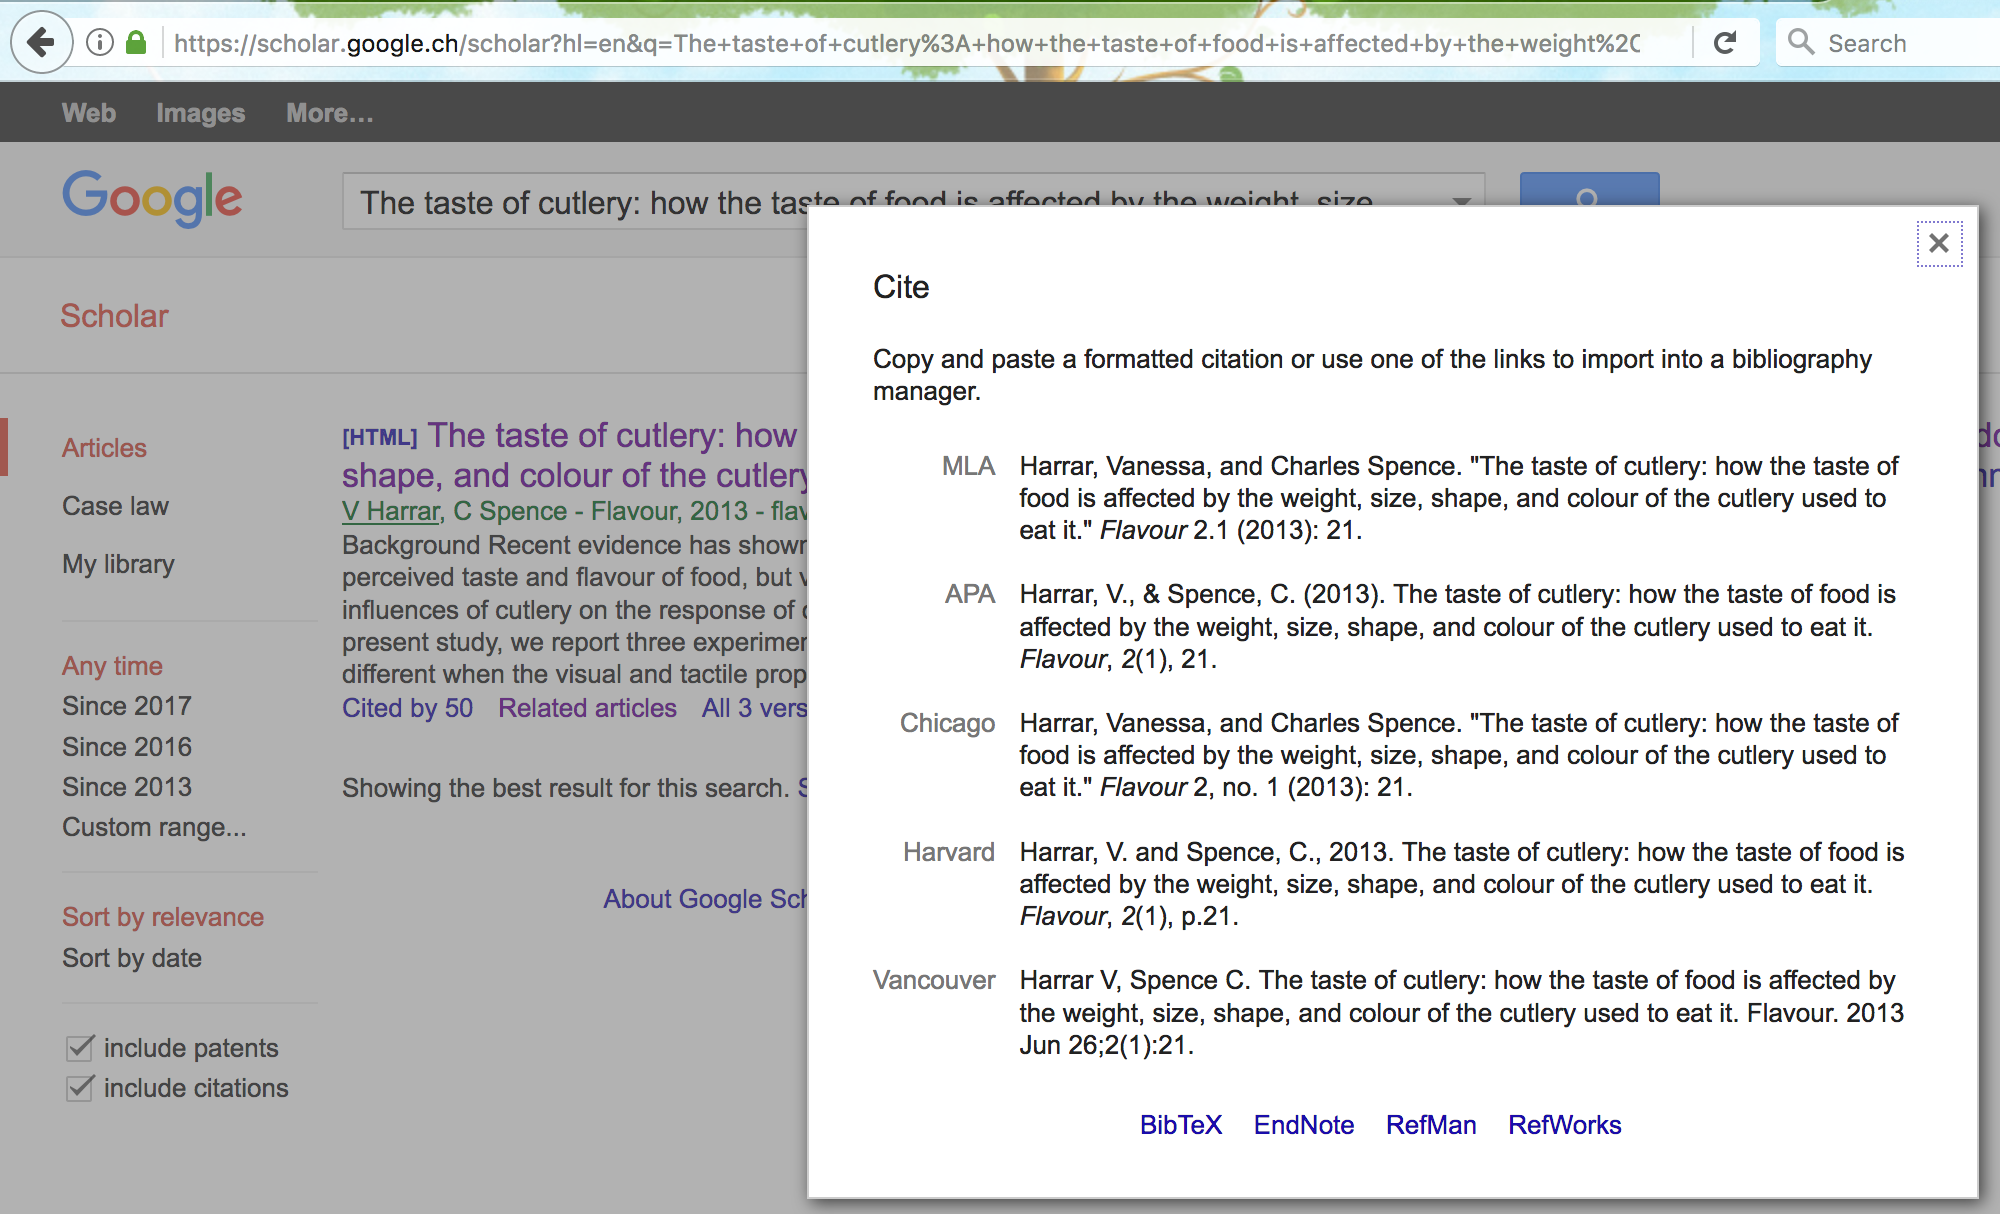
\includegraphics{images/googlescholar2.png}

For ``.bib'' files we are interested in the ``BibTeX'' option and by
clicking on it we will be taken to another tab in which the format of
the reference we want is provided. All that needs to be done at this
point is to copy this format (that we saw earlier in this section) and
paste in the ``.bib'' file you created and save the changes.

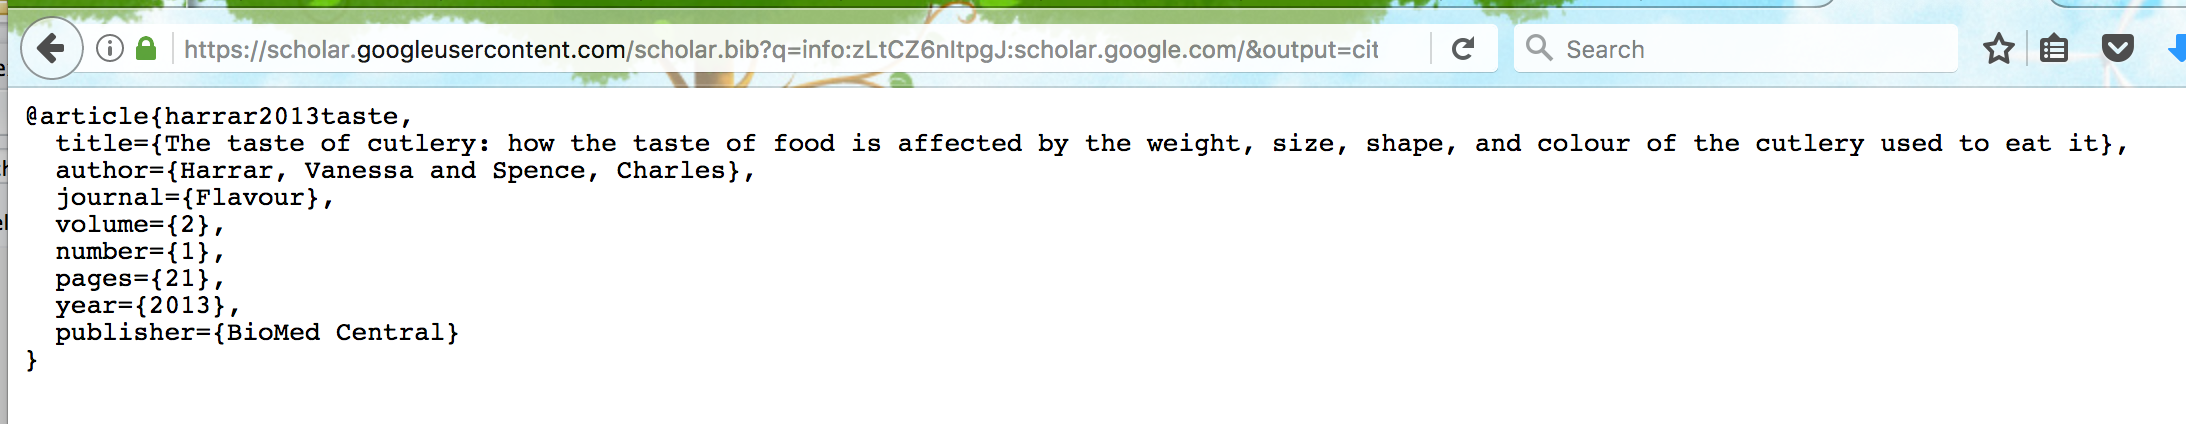
\includegraphics{images/googlescholar3.png}

However, your RMarkdown document does not know about the existence of
this bibliography file and therefore we need to insert this information
in the YAML metadata at the start of our document. To do so, let us
suppose that you named this file ``biblio.bib'' (saved in the same
location as your RMarkdown document). All that needs to be done is to
add another line in the YAML metadata with
\texttt{bibliography:\ biblio.bib} and your RMarkdown will now be able
to recognize the references within your ``.bib'' file.

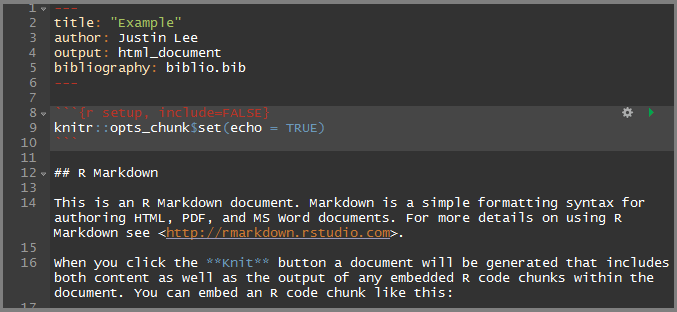
\includegraphics{images/rmd_yaml2.png}

There are also a series of other options that can be specified for the
bibliography such as its format or the way references can be used within
the text (see links at the end of this section).

Once the ``.bib'' file has been created and has been linked to your
RMarkdown document through the details in the YAML metadata, you can now
start using the references you have collected in the ``.bib'' file. To
insert these references within your document at any point of your text
you need to use the name that starts the reference field in your
``.bib'' file and place it immediately after the \texttt{@} symbol
(without spaces). So, for example, say that we wanted to cite the
publication on the ``taste of cutlery'': in your RMarkdown all you have
to do is to type \texttt{@harrar2013taste} at the point where you want
this citation in the text and you will obtain: \citet{harrar2013taste}.
Moreover, it is often useful to put a citation in braces and for example
if you want to obtain \citep[see e.g.][]{harrar2013taste} you can simply
write \texttt{{[}see\ e.g.\ @harrar2013taste{]}}.

\BeginKnitrBlock{rmdnote}
The user can also change the name that is used to call the desired
reference as long as the same name is used to cite it in the RMarkdown
document and that this name is not the same as another reference.
\EndKnitrBlock{rmdnote}

\BeginKnitrBlock{rmdcaution}
The references in the ``.bib'' file will not appear in the references
that are output from the RMarkdown compiling procedure unless they are
specifically used within the RMarkdown document.
\EndKnitrBlock{rmdcaution}

Additional information on BibTeX and reference in RMarkdown can be found
in the links below:

\begin{itemize}
\tightlist
\item
  \href{https://www.economics.utoronto.ca/osborne/latex/BIBTEX.HTM}{Introduction
  to bibtex}
\item
  \href{http://RMarkdown.rstudio.com/authoring_bibliographies_and_citations.html}{Reference
  in RMarkdown}
\end{itemize}

\subsection{Tables}\label{tables}

For simple tables, we can be manually insert values as such follows:

\begin{verbatim}
+---------------+---------------+--------------------+
| Fruit         | Price         | Advantages         |
+===============+===============+====================+
| *Bananas*     | $1.34         | - built-in wrapper |
|               |               | - bright color     |
+---------------+---------------+--------------------+
| Oranges       | $2.10         | - cures scurvy     |
|               |               | - **tasty**        |
+---------------+---------------+--------------------+
\end{verbatim}

to produce:

\begin{longtable}[]{@{}lll@{}}
\toprule
\begin{minipage}[b]{0.20\columnwidth}\raggedright\strut
Fruit\strut
\end{minipage} & \begin{minipage}[b]{0.20\columnwidth}\raggedright\strut
Price\strut
\end{minipage} & \begin{minipage}[b]{0.27\columnwidth}\raggedright\strut
Advantages\strut
\end{minipage}\tabularnewline
\midrule
\endhead
\begin{minipage}[t]{0.32\columnwidth}\raggedright\strut
\emph{Bananas}\strut
\end{minipage} & \begin{minipage}[t]{0.32\columnwidth}\raggedright\strut
\$1.34\strut
\end{minipage} & \begin{minipage}[t]{0.32\columnwidth}\raggedright\strut
\begin{itemize}
\tightlist
\item
  built-in wrapper
\item
  bright color
\end{itemize}\strut
\end{minipage}\tabularnewline
\begin{minipage}[t]{0.32\columnwidth}\raggedright\strut
Oranges\strut
\end{minipage} & \begin{minipage}[t]{0.32\columnwidth}\raggedright\strut
\$2.10\strut
\end{minipage} & \begin{minipage}[t]{0.32\columnwidth}\raggedright\strut
\begin{itemize}
\tightlist
\item
  cures scurvy
\item
  \textbf{tasty}
\end{itemize}\strut
\end{minipage}\tabularnewline
\bottomrule
\end{longtable}

As an alternative we can use the simple graphical user interface
\href{http://www.tablesgenerator.com/markdown_tables}{online}. For more
extensive tables, we create dataframe objects and project them using
\texttt{knitr::kable()} which we will explain later on this book.

\subsection{Additional References}\label{additional-references-1}

There are many more elements to creating a useful report using
RMarkdown, and we encourage you to use the
\href{https://www.rstudio.com/wp-content/uploads/2015/02/rmarkdown-cheatsheet.pdf}{RMarkdown
Cheatsheet} as a reference.

\section{Code Chunks}\label{code-chunks}

Code chunks are those parts of the RMarkdown document where it is
possible to embed R code within your output. To insert these chunks
within your RMarkdown file you can use the following shortcuts:

\begin{itemize}
\tightlist
\item
  the keyboard shortcut Ctrl + Alt + I (OS X: Cmd + Option + I)
\item
  the Add Chunk command in the editor toolbar
\item
  by typing the chunk delimiters \textbf{```\{\r\}} and \textbf{```}.
\end{itemize}

The following example highlights the code chunks in the example
RMarkdown document we saw at the start of this chapter:

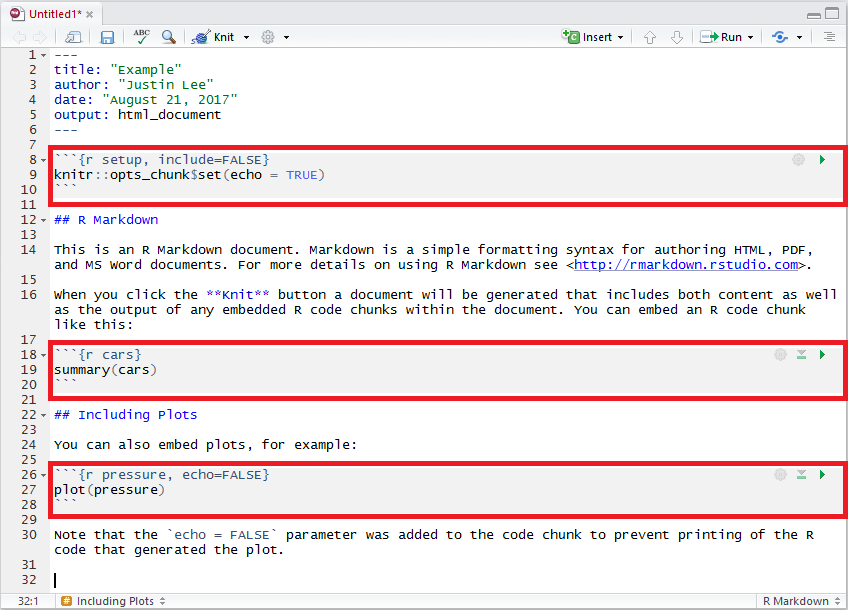
\includegraphics{images/rmd_code_chunk.png}

\subsection{Code Chunk Options}\label{code-chunk-options}

A variety of options can be specified to manage the code chunks
contained in the document. For example, as can be seen in the third code
chunk in the example above, we specify an argument that reads
\texttt{echo\ =\ FALSE} which is a parameter that was added to the code
chunk to prevent printing the R code that generated the plot. This is a
useful way to embed figures. More options can be found from the
\href{https://www.rstudio.com/wp-content/uploads/2015/02/rmarkdown-cheatsheet.pdf}{RMarkdown
Cheatsheet} and Yihui's notes on knitr
\href{https://yihui.name/knitr/options/}{options}. Here are some
explanations of the most commonly used chunk options taken from these
references:

\begin{itemize}
\tightlist
\item
  \texttt{eval}: (TRUE; logical) whether to evaluate the code chunk;
\item
  \texttt{echo}: (TRUE; logical or numeric) whether to include R source
  code in the output file;
\item
  \texttt{warning}: (TRUE; logical) whether to preserve warnings
  (produced by warning()) in the output like we run R code in a terminal
  (if FALSE, all warnings will be printed in the console instead of the
  output document);
\item
  \texttt{cache}: (FALSE; logical) whether to ``\emph{cache}'' a code
  chunk. This option is particularly important in practice and is
  discussed in more details in Section \ref{cache}.
\end{itemize}

Plot figure options:

\begin{itemize}
\tightlist
\item
  \texttt{fig.path}: (`figure/'; character) prefix to be used for figure
  filenames (fig.path and chunk labels are concatenated to make
  filenames);
\item
  \texttt{fig.show}: (`asis'; character) how to show/arrange the plots;
\item
  \texttt{fig.width}, \texttt{fig.height}: (both are 7; numeric) width
  and height of the plot, to be used in the graphics device (in inches)
  and have to be numeric;
\item
  \texttt{fig.align}: (`default'; character) alignment of figures in the
  output document (possible values are left, right and center;
\item
  \texttt{fig.cap}: (NULL; character) figure caption to be used in a
  figure environment.
\end{itemize}

\subsection{Comments}\label{comments}

Adding comments to describe the code is extremely useful (if not
essential) during every coding and programming process. It helps
\textbf{you} take notes and remember what is going on and why you made
use of these functions, as well as helping others understand your code.
Forgetting to comment or document your code often becomes a larger
problem in the future when, among numerous lines of code, you have
forgotten the reason for using certain functions or algorithms.

\begin{quote}
``Don't document bad code -- rewrite it.'' The Elements of Programming
Style, Kernighan \& Plauger
\end{quote}

\begin{Shaded}
\begin{Highlighting}[]
\CommentTok{# Comment your code by preceding text with a # }
\CommentTok{# Keep it brief but comprehensible, so you can return to it }
\end{Highlighting}
\end{Shaded}

\subsection{In-line R}\label{in-line-r}

The variables we store in an RMarkdown document will stay within the
environment they were created in. This means that we can call and
manipulate them anywhere within the document. For example, supposing we
have a variable called \texttt{x} to which we assign a specific value,
then in RMarkdown we can reference this variable by using \texttt{r\ x}:
this will affix the value of the variable directly in a sentence. Here
is a practical example:

\begin{Shaded}
\begin{Highlighting}[]
\NormalTok{a <-}\StringTok{ }\DecValTok{2}
\end{Highlighting}
\end{Shaded}

where we have stored the value 2 in a variable called \texttt{a}. We can
use the value of \texttt{a} as follows:

\begin{verbatim}
The value of $a$ is `r a`. 
\end{verbatim}

This translates in R Markdown to ``The value of \(a\) is 2.''

\subsection{Cache}\label{cache}

Depending on the complexity of calculations in your embedded R code, it
may be convenient to avoid re-running the computations (which could be
lengthy) each time you knit the document together. For this purpose, it
possible to specify an additional argument for your embedded R code
which is the \texttt{cache} argument. By default this argument is
assigned the value \texttt{FALSE} and therefore the R code is run every
time your document is compiled. However, if you specify this argument as
\texttt{cache\ =\ TRUE}, then the code is only run the first time the
document is compiled while the following times it simply stores and
presents the results of the computations when the document was first
compiled.

Below is a short video introducing caching in R Markdown.

The RMarkdown file used for this particular example can be found here:
\href{code_examples/caching.Rmd}{caching.Rmd}.

Let us consider an example where we want to embed an R code with a very
simple operation such as assigning the value of 2 to an object that we
call \texttt{a} (that we saw earlier). This is clearly not the best
example since this operation runs extremely quickly and there is no
visible loss in document compilation time. However, we will use it just
to highlight how the \texttt{cache} argument works. Therefore, if we
want to avoid running this operation each time the document is compiled,
then we just embed our R code as follows:

\begin{Shaded}
\begin{Highlighting}[]
\NormalTok{a <-}\StringTok{ }\DecValTok{2}
\end{Highlighting}
\end{Shaded}

which would be written in RMarkdown as:

\begin{Shaded}
\begin{Highlighting}[]
\StringTok{```}\DataTypeTok{\{r computeA, cache = TRUE\}}
\DataTypeTok{a <- 2}
\StringTok{```}
\end{Highlighting}
\end{Shaded}

You will notice that we called this chunk of embedded R code
\texttt{computeA} and the reason for this will become apparent further
on. Once we have done this we can compile the document that will run
this operation and store its result. Now, if we compile the document
again (independently from whether we made changes to the rest of the
document or not) this operation will not be run and the result of the
previous (first) compiling will be presented. However, if changes are
made to the R code which has been ``cached'', then the code will be run
again and this time its new result will be stored for all the following
compilings until it is changed again.

This argument can therefore be very useful when computationally
intensive R code is embedded within your document. Nevertheless it can
suffer from a drawback which consists in dependencies of your ``cached''
R code with other chunks within the document. In this case, the other
chunks of R code can be modified thereby outputting different results
but these will not be considered by your ``cached'' R code. As an
example, suppose we have another chunk of R code that we can ``cache''
and that takes the value of \texttt{a} from the previous chunk:

\begin{Shaded}
\begin{Highlighting}[]
\NormalTok{(d <-}\StringTok{ }\DecValTok{2}\OperatorTok{*}\NormalTok{a)}
\end{Highlighting}
\end{Shaded}

\begin{verbatim}
## [1] 4
\end{verbatim}

which would be written in RMarkdown as:

\begin{Shaded}
\begin{Highlighting}[]
\StringTok{```}\DataTypeTok{\{r, cache = TRUE\}}
\DataTypeTok{(d <- 2*a)}
\StringTok{```}
\end{Highlighting}
\end{Shaded}

In this case, the output of this chunk will be \texttt{\#\#\ 4} since
\texttt{a\ \textless{}-\ 2} (from the previous chunk). What happens
however if we modify the value of \texttt{a} in the previous chunk? In
this case, the previous chunk will be recomputed but the value of
\texttt{d} (in the following chunk) will not be updated since it has
stored the value of 4 and it is not recomputed since this chunk has not
been modified. To avoid this, a solution is to specify the chunks of
code that the ``cached'' code depends on. This is why we initially gave
a name to the first chunk of code (``computeA'') so as to refer to it in
following chunks of ``cached'' code that depend on it. To refer to this
code you need to use the option \texttt{dependson} as follows:

\begin{Shaded}
\begin{Highlighting}[]
\NormalTok{(d <-}\StringTok{ }\DecValTok{2}\OperatorTok{*}\NormalTok{a)}
\end{Highlighting}
\end{Shaded}

\begin{verbatim}
## [1] 4
\end{verbatim}

which we would write as:

\begin{Shaded}
\begin{Highlighting}[]
\StringTok{```}\DataTypeTok{\{r, cache = TRUE, dependson = "computeA"\}}
\DataTypeTok{(d <- 2*a)}
\StringTok{```}
\end{Highlighting}
\end{Shaded}

In this manner, if the value of \texttt{a} changes in the first chunk,
the value of \texttt{d} will also change but will be stored until either
the \texttt{computeA} chunk or the latter chunk is modified.

\section{Render Output}\label{render-output}

After you are done, run \texttt{RMarkdown::render()} or click the
\texttt{Knit} button at the top of the RStudio scripts pane to save the
output in your working directory.

\begin{figure}
\centering
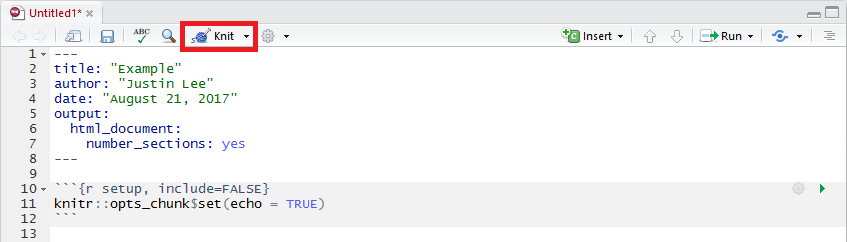
\includegraphics{images/rmd_knit.png}
\caption{}
\end{figure}

The use of RMarkdown makes it possible to generate any file format such
as HTML, pdf and Word processor formats using \texttt{pandoc}. Pandoc is
a free software that understands and converts useful markdown syntax,
such as the code mentioned above, into a readable and clean format.

\section{Addition Information}\label{addition-information}

Click on the links below for more information on RMarkdown:

\begin{itemize}
\tightlist
\item
  \href{http://RMarkdown.rstudio.com/authoring_quick_tour.html}{RStudio
  RMarkdown tutorial}
\item
  \href{https://www.r-bloggers.com/r-markdown-and-knitr-tutorial-part-1/}{R-blogger's
  RMarkdown tutorial}
\item
  \href{https://www.rstudio.com/wp-content/uploads/2015/02/rmarkdown-cheatsheet.pdf}{RMarkdown
  Cheatsheet}
\end{itemize}

\chapter{GitHub}\label{github}

When working on a report or a project, it is often the case that you
keep separate versions either to keep track of the changes (in case you
want to go back to a previous version) or to have a version for each
person working on different parts of the project. As a result of this
approach, you may have experienced a moment like this at least once in
your life:

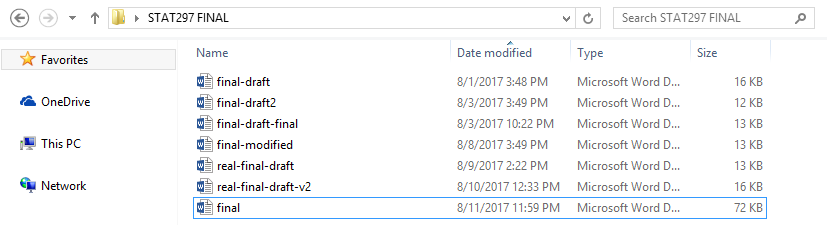
\includegraphics{images/bad-version-control.png}

In these cases, after having modified and changed different parts of a
report, you probably find yourself saving the same file over and over
again while losing track of what changes you made. To respond to this
problem, software has been developed to keep track of your changes by
informing you on the saves you made and allowing you to go back to
previous versions in order to revert those changes. This software is
generally called ``version control'' and this chapter discusses the
features of this software as well as introducing a specific version
control platform called ``GitHub''. The latter includes a series of
highly useful tools that can be extremely helpful, not only for the
projects developed based on this book, but also for any personal or
collaborative project you may undertake in the future.

\section{Version Control}\label{version-control}

As mentioned above, \emph{version control} is a system that records
changes to a file or a set of files in order to keep track and possibly
revert to or modify those changes over time. More specifically, it
allows you to:

\begin{itemize}
\tightlist
\item
  record the entire history of a file;
\item
  revert to a specific version of the file;
\item
  collaborate on the same platform with other people;
\item
  make changes without modifying the main file and add them once you
  feel comfortable with them.
\end{itemize}

All these features are highly important when projects start becoming
more complex and/or different collaborators contribute to it. In the
next section we present a version control platform called ``GitHub''
that is commonly used among programmers and software developers thereby
allowing them also to make their work visible and available to the
general public.

\section{Git and GitHub}\label{git-and-github}

Among the different version control platforms, Git is a commonly used
and powerful tool that is made more accessible through GitHub which is a
commercial website. The latter uses the Git platform and stores local
files into a flexible folder called a ``repository''. For the purposes
of this course, we will be using this platform and in the following
sections we will briefly describe how to install and get started with
this version control platform.

Below is a video introducing GitHub.

\subsection{Git Setup}\label{git-setup}

To install Git, go to the \href{https://git-scm.com/downloads}{website}
and select the version which is compatible with the OS of your computer
(e.g.~Windows/Mac/Linux/Solaris). Once you've downloaded and installed
Git, the first thing you should do is to configure it by setting your
username and email address. This is important because each time you
interact with the platform and upload (commit) your changes to Git, this
information is used to synchronize versions and keep track of project
evolution.

\subsubsection{Tell Git Who You Are}\label{tell-git-who-you-are}

Once you have installed Git, run the \texttt{Git\ Bash} software and
type the following code below.

\begin{verbatim}
$ git config --global user.name "John Doe"
$ git config --global user.email johndoe@example.com
\end{verbatim}

This is the initial configuration of your author name and email address
for your commits. You may need to do this before you begin pushing and
pulling with your current account information. This operation only needs
to be done once when using the ``--global'' option because, in this
case, Git will always use that information for anything you do on that
system. If you want to override this with a different name or email
address for specific projects, you can run the command without the
``--global'' option while working on those projects.

\subsection{GitHub Setup}\label{github-setup}

In order to set up GitHub, go to the \href{https://github.com/}{GitHub
website} and, for the purposes of the course, the first step is to sign
up with your University email address.

\BeginKnitrBlock{rmdnote}
Your username and email can be changed at any time so, if you want to
change it, you can easily do so once this course is over.
\EndKnitrBlock{rmdnote}


\includegraphics{images/github_page.png}

Once this is done, you reach \texttt{Step\ 2:\ Choose\ your\ plan} where
you can choose the default plan (``Unlimited public repositories for
free'') and click \texttt{Continue}. The last (optional) step is
\texttt{Step\ 3:\ Tailor\ your\ experience} which allows you to submit
your information but this can also be skipped.

\BeginKnitrBlock{rmdnote}
Your GitHub profile can also serve as a \emph{resume} of your data
science skills that will be highlighted by possible future projects that
you save and commit.
\EndKnitrBlock{rmdnote}

\subsection{Student Developer Pack}\label{student-developer-pack}

As a student, it is possible to benefit from specific advantages when
using GitHub. Indeed, once you have set up your profile you can go to
this \href{https://education.github.com/discount_requests/new}{link} and
follow the steps below to set up a ``student developer pack'' discount
request to GitHub. Through this setup it will be possible for you not
only to have free \emph{public} repositories but also to make your own
\emph{private} repositories for free.


\includegraphics{images/developer_pack.png}

\section{GitHub Workflow}\label{github-workflow}

Here is a video demonstrating the basic GitHub workflow in GitHub
Desktop (initializing, committing, pushing and pulling) that we will
follow for our assignments and projects.

In addition, here is a video demonstrating the basic GitHub workflow
within RStudio.

While the main features and actions to manage the workflow in GitHub are
desribed in the above videos, the following paragraphs give some extra
details that can be helpful to consider when working with this
version-control platform.

\subsection{Branching}\label{branching}

In the previous section we discussed the workflow as a means of directly
making changes in the so-called \emph{master} branch which is where our
original and up-to-date work is stored. However, when working with
different collaborators for example, it may be appropriate to create
separate branches that will avoid modifying the original one until
you're sure of the changes. In this perspective, \emph{branching} is
essentially creating an environment in which we can change anything
without obstructing our original document. As mentioned, this idea is
very useful for group-based activities where different people are
working on the same files. Once we have made all our changes and are
sure of the changes, we can merge the changes to the main
\texttt{master} branch. You can learn more about branching
\href{https://git-scm.com/book/en/v1/Git-Branching-Basic-Branching-and-Merging}{here}
and \href{https://gist.github.com/vlandham/3b2b79c40bc7353ae95a}{here}.

\subsection{Pull}\label{pull}

Before starting (or continuing) to work on your project, make sure to
always review changes that another collaborator has made. Once this is
done you can make sure there are no merge conflicts and you can pull (or
synchronize) your local branch with the most recent version of the
repository. If merge conflicts were to happen, these can still be solved
but it would be preferable to avoid them generating confusion.

\subsection{Commits}\label{commits}

After we have created the branch, we can start modifying the documents
(add, edit, or delete) within the repository. Once these changes are
made, you need to \texttt{commit} them with an informative message,
explaining why a particular change is being made. These specific
messages allow you to backtrack on these changes later if you decide to
look at the history of any of these files and find a bug. This
information is extremely important since otherwise there's little point
in using version control like GitHub. \footnote{This scheme is inspired
  from diagrams by Prof.~Bob Rudis and James Balamuta.}

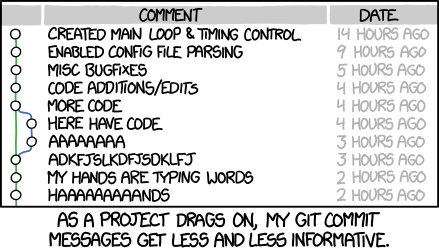
\includegraphics{images/git_commit.png}

\subsubsection{Pull Request}\label{pull-request}

If you are directly working on the master branch, please disregard this
section. Else, a \texttt{pull\ request} may be made by the person
working on the branch, so that other collaborators can discuss about the
commits made in the branch. Also, there are options for conversation in
which they can review and comment directly onto the code as well.

\subsection{Push or Merge}\label{push-or-merge}

Once you have either made the commits on your master branch or have the
pull request confirmed by other collaborators, you can merge or push the
changes into the remote master branch. This means that the version of
the repository online will have your updated code and documents. This
will be the final step to the cycle of the workflow after which we can
clear and repeat the above procedure.

\subsection{Merge Conflicts}\label{merge-conflicts}

Merge conflicts often occur when two different collaborators make
different changes to the same line of a file, and also can happen when a
file that is meant to be modified is deleted (although these may not be
the only situations). To resolve these conflicts, we must directly edit
the documents making sure potential conflicts are discussed before
merging or pushing to the master branch, since merge conflicts often
occur from miscommunication within groups.

\section{GitHub Workflow on Command Line / Git
Bash}\label{github-workflow-on-command-line-git-bash}

Here are commands that we can use within \texttt{Git\ Bash} if we are
more comfortable working on the command line.

\begin{longtable}[]{@{}ll@{}}
\toprule
Command & Function\tabularnewline
\midrule
\endhead
git init & Create a \textbf{local} repository\tabularnewline
git branch ``newbranch'' & Create a new branch with given
name\tabularnewline
git checkout ``newbranch'' & Switch to specified branch\tabularnewline
git status & List all the files that you have modified\tabularnewline
git add -A & Add \textbf{all} files to staging\tabularnewline
git commit -m ``commit message'' & Commit staged changes to
\textbf{local} repository\tabularnewline
git push & Commit saved changes to \textbf{remote}
repository\tabularnewline
git pull & Update changes from the \textbf{remote}
repository\tabularnewline
\bottomrule
\end{longtable}

However, it is better for us to startby using more graphical
user-interface options since they allow us to better understand what is
going on. You \textbf{do not} want to follow this example\footnote{\url{https://xkcd.com/1597/}}\ldots{}


\includegraphics{images/git_misuse.png}

It is always important to know what is happening when we create, change,
push, branch and pull from a repository.

\section{Issues}\label{issues}

\emph{Issues} are a very good way to keep track of group tasks, bugs and
announcements for your projects within GitHub. Below is a basic video
introducing \texttt{issues} in GitHub.

\section{Slack Integration}\label{slack-integration}

Slack is a platform created to communicate between group members,
allowing for both direct individual messages as well as group messages.
More information on how to use Slack can be found in this
\href{https://get.slack.help/hc/en-us/articles/218080037-Getting-started-for-new-members}{Slack
Tutorial}.

An added benefit of using Slack is that it can be integrated with GitHub
in such a way that notifications will be posted to the group whenever
someone pushes or makes a pull request. More information on GitHub
integration with Slack can be found
\href{https://get.slack.help/hc/en-us/articles/232289568-Use-GitHub-with-Slack}{here}.

A more detailed video providing a demonstration on the use of Slack in a
real-life setting can be found below.

\section{Additional References}\label{additional-references-2}

Below are some supplemental references that can support you in a better
use of GitHub.

\begin{itemize}
\tightlist
\item
  \href{https://www.r-bloggers.com/rstudio-and-github/}{GitHub
  Introduction with RStudio}
\item
  \href{https://guides.github.com/introduction/flow/}{GitHub Workflow}
\item
  \href{https://www.youtube.com/watch?v=oFYyTZwMyAg}{GitHub on Command
  Line (video)}
\end{itemize}

\part{Introduction to R}\label{part-introduction-to-r}

\chapter{Data Structures}\label{data}

There are different data types that are commonly used in R among which
the most important ones are the following:

\begin{itemize}
\item
  \textbf{Numeric} (or double): these are used to store real numbers.
  Examples: -4, 12.4532, 6.
\item
  \textbf{Integer}: examples: 2L, 12L.
\item
  \textbf{Logical} (or boolean): examples: \texttt{TRUE},
  \texttt{FALSE}.
\item
  \textbf{Character}: examples: \texttt{"a"}, \texttt{"Bonjour"}.
\end{itemize}

In R there are five types of data structures in which elements can be
stored. A data structure is said to \emph{homogeneous} if it only
contains elements of the same type (for example it only contains
character or only numeric values) and \emph{heterogenous} if it contains
elements of more than one type. The five types of data structures are
commonly summarized in a table similar to the one below \citep[see
e.g.][]{wickham2014advanced}:

\begin{longtable}[]{@{}lcc@{}}
\caption{\label{tab:ds} Five most common types of data structures used in R
\citep{wickham2014advanced}.}\tabularnewline
\toprule
Dimension & Homogenous & Heterogeneous\tabularnewline
\midrule
\endfirsthead
\toprule
Dimension & Homogenous & Heterogeneous\tabularnewline
\midrule
\endhead
1 & Vector & List\tabularnewline
2 & Matrix & Data Frame\tabularnewline
n & Array &\tabularnewline
\bottomrule
\end{longtable}

Consider a simple data set of the top five male single tennis players
presented below:

\begin{longtable}[]{@{}ccccclll@{}}
\caption{\label{tab:tennis} Five best male single tennis players as ranked
by ATP (07-15-2017).}\tabularnewline
\toprule
Name & Date of Birth & Born & Country & ATP Ranking & Prize Money & Win
Percentage & Grand Slam Wins\tabularnewline
\midrule
\endfirsthead
\toprule
Name & Date of Birth & Born & Country & ATP Ranking & Prize Money & Win
Percentage & Grand Slam Wins\tabularnewline
\midrule
\endhead
Andy Murray & 15 May 1987 & Glasgow, Scotland & Great Britain & 1 &
60,449,649 & 78.07 & 9\tabularnewline
Rafael Nadal & 3 June 1986 & Manacor, Spain & Spain & 2 & 85,920,132 &
82.48 & 15\tabularnewline
Stan Wawrinka & 28 March 1985 & Lausanne, Switzerland & Switzerland & 3
& 30,577,981 & 63.96 & 5\tabularnewline
Novak Djokovic & 22 May 1987 & Belgrade, Serbia & Serbia & 4 &
109,447,408 & 82.77 & 12\tabularnewline
Roger Federer & 8 August 1981 & Basel, Switzerland & Switzerland & 5 &
104,445,185 & 81.80 & 18\tabularnewline
\bottomrule
\end{longtable}

Notice that this data set contains a variety of data types; in the next
sections we will use this data to illustrate how to work with five
common data structures.

\section{Vectors}\label{vectors}

A vector has three important properties:

\BeginKnitrBlock{rmdimportant}
\begin{itemize}
\tightlist
\item
  The \textbf{Type} of objects contained in the vector. The function
  \texttt{typeof()} returns a description of the type of objects in a
  vector.
\item
  The \textbf{Length} of a vector indicates the number of elements in
  the vector. This information can be obtained using the function
  \texttt{length()}.
\item
  \textbf{Attributes} are metadata attached to a vector. The functions
  \texttt{attr()} and \texttt{attributes()} can be used to store and
  retrieve attributes (more details can be found in Section
  \ref{vectattr}).\\
\end{itemize}
\EndKnitrBlock{rmdimportant}

\texttt{c()} is a generic function that combines arguments to form a
vector. All arguments are coerced to a common type (which is the type of
the returned value) and all attributes except names are removed. For
example, consider the number of grand slams won by the five players
considered in the eighth column of Table \ref{tab:tennis}:

\begin{Shaded}
\begin{Highlighting}[]
\NormalTok{grand_slam_win <-}\StringTok{ }\KeywordTok{c}\NormalTok{(}\DecValTok{9}\NormalTok{, }\DecValTok{15}\NormalTok{, }\DecValTok{5}\NormalTok{, }\DecValTok{12}\NormalTok{, }\DecValTok{18}\NormalTok{)}
\end{Highlighting}
\end{Shaded}

To display the values stored in \texttt{grand\_slam\_win} we could
simply enter the following in the R console:

\begin{Shaded}
\begin{Highlighting}[]
\NormalTok{grand_slam_win}
\end{Highlighting}
\end{Shaded}

\begin{verbatim}
## [1]  9 15  5 12 18
\end{verbatim}

Alternatively, we could have created and displayed the value by using
\texttt{()} around the definition of the object itself as follows:

\begin{Shaded}
\begin{Highlighting}[]
\NormalTok{(grand_slam_win <-}\StringTok{ }\KeywordTok{c}\NormalTok{(}\DecValTok{9}\NormalTok{, }\DecValTok{15}\NormalTok{, }\DecValTok{5}\NormalTok{, }\DecValTok{12}\NormalTok{, }\DecValTok{18}\NormalTok{))}
\end{Highlighting}
\end{Shaded}

\begin{verbatim}
## [1]  9 15  5 12 18
\end{verbatim}

Various forms of ``nested concatenation'' can be used to define vectors.
For example, we could also define \texttt{grand\_slam\_win} as

\begin{Shaded}
\begin{Highlighting}[]
\NormalTok{(grand_slam_win <-}\StringTok{ }\KeywordTok{c}\NormalTok{(}\DecValTok{9}\NormalTok{, }\KeywordTok{c}\NormalTok{(}\DecValTok{15}\NormalTok{, }\DecValTok{5}\NormalTok{, }\KeywordTok{c}\NormalTok{(}\DecValTok{12}\NormalTok{, }\KeywordTok{c}\NormalTok{(}\DecValTok{18}\NormalTok{)))))}
\end{Highlighting}
\end{Shaded}

\begin{verbatim}
## [1]  9 15  5 12 18
\end{verbatim}

This approach is often used to assemble vectors in various ways.

It is also possible to define vectors with characters, for example we
could define a vector with the player names as follows:

\begin{Shaded}
\begin{Highlighting}[]
\NormalTok{(players <-}\StringTok{ }\KeywordTok{c}\NormalTok{(}\StringTok{"Andy Murray"}\NormalTok{, }\StringTok{"Rafael Nadal"}\NormalTok{, }\StringTok{"Stan Wawrinka"}\NormalTok{, }
             \StringTok{"Novak Djokovic"}\NormalTok{, }\StringTok{"Roger Federer"}\NormalTok{))}
\end{Highlighting}
\end{Shaded}

\begin{verbatim}
## [1] "Andy Murray"    "Rafael Nadal"   "Stan Wawrinka"  "Novak Djokovic"
## [5] "Roger Federer"
\end{verbatim}

\subsection{Type}\label{type}

We can evaluate the kind or type of elements that are stored in a vector
using the function \texttt{typeof()}. For example, for the vectors we
just created we obtain:

\begin{Shaded}
\begin{Highlighting}[]
\KeywordTok{typeof}\NormalTok{(grand_slam_win)}
\end{Highlighting}
\end{Shaded}

\begin{verbatim}
## [1] "double"
\end{verbatim}

\begin{Shaded}
\begin{Highlighting}[]
\KeywordTok{typeof}\NormalTok{(players)}
\end{Highlighting}
\end{Shaded}

\begin{verbatim}
## [1] "character"
\end{verbatim}

This is a little surprising since all the elements in
\texttt{grand\_slam\_win} are integers and it would seem natural to
expect this as an output of the function \texttt{typeof()}. This is
because R considers any number as a ``double'' by default, except when
adding the suffix \texttt{L} after an integer. For example:

\begin{Shaded}
\begin{Highlighting}[]
\KeywordTok{typeof}\NormalTok{(}\DecValTok{1}\NormalTok{)}
\end{Highlighting}
\end{Shaded}

\begin{verbatim}
## [1] "double"
\end{verbatim}

\begin{Shaded}
\begin{Highlighting}[]
\KeywordTok{typeof}\NormalTok{(1L)}
\end{Highlighting}
\end{Shaded}

\begin{verbatim}
## [1] "integer"
\end{verbatim}

Therefore, we could express \texttt{grand\_slam\_win} as follows:

\begin{Shaded}
\begin{Highlighting}[]
\NormalTok{(grand_slam_win_int <-}\StringTok{ }\KeywordTok{c}\NormalTok{(9L, 15L, 5L, 12L, 18L))}
\end{Highlighting}
\end{Shaded}

\begin{verbatim}
## [1]  9 15  5 12 18
\end{verbatim}

\begin{Shaded}
\begin{Highlighting}[]
\KeywordTok{typeof}\NormalTok{(grand_slam_win_int)}
\end{Highlighting}
\end{Shaded}

\begin{verbatim}
## [1] "integer"
\end{verbatim}

In general, the difference between the two is relatively unimportant.

\subsection{Coercion}\label{coercion}

As indicated earlier, a vector has a homogeneous data structure meaning
that it can only contain a single type among all the data types.
Therefore, when more than one data type is provided, R will
\emph{coerce} the data into a ``shared'' type. To identify this
``shared'' type we can use this simple rule:

\begin{equation*}
 \text{logical} < \text{integer} < \text{numeric} < \text{character},
\end{equation*}

which simply means that if a vector has more than one data type, the
``shared'' type will be that of the ``largest'' type according to the
progression shown above. For example:

\begin{Shaded}
\begin{Highlighting}[]
\CommentTok{# Logical + numeric}
\NormalTok{(mix_logic_int <-}\StringTok{ }\KeywordTok{c}\NormalTok{(}\OtherTok{TRUE}\NormalTok{, }\DecValTok{12}\NormalTok{, }\FloatTok{0.5}\NormalTok{))}
\end{Highlighting}
\end{Shaded}

\begin{verbatim}
## [1]  1.0 12.0  0.5
\end{verbatim}

\begin{Shaded}
\begin{Highlighting}[]
\KeywordTok{typeof}\NormalTok{(mix_logic_int)}
\end{Highlighting}
\end{Shaded}

\begin{verbatim}
## [1] "double"
\end{verbatim}

\begin{Shaded}
\begin{Highlighting}[]
\CommentTok{# Numeric + character}
\NormalTok{(mix_int_char <-}\StringTok{ }\KeywordTok{c}\NormalTok{(}\FloatTok{14.3}\NormalTok{, }\StringTok{"Hi"}\NormalTok{))}
\end{Highlighting}
\end{Shaded}

\begin{verbatim}
## [1] "14.3" "Hi"
\end{verbatim}

\begin{Shaded}
\begin{Highlighting}[]
\KeywordTok{typeof}\NormalTok{(mix_int_char)}
\end{Highlighting}
\end{Shaded}

\begin{verbatim}
## [1] "character"
\end{verbatim}

\subsection{Subsetting}\label{subsetting}

Naturally, it is possible to ``subset'' the values of in our vector in
many ways. Essentially, there are four main ways to subset a vector.
Here we'll only discuss the first three:

\begin{itemize}
\tightlist
\item
  \textbf{Positive Index}: We can \emph{access} or \emph{subset} the
  \(i\)-th element of a vector by simply using
  \texttt{grand\_slam\_win{[}i{]}} where \(i\) is a positive number
  between 1 and the length of the vector.
\end{itemize}

\begin{Shaded}
\begin{Highlighting}[]
\CommentTok{# Accessing the first element}
\NormalTok{grand_slam_win[}\DecValTok{1}\NormalTok{]}
\end{Highlighting}
\end{Shaded}

\begin{verbatim}
## [1] 9
\end{verbatim}

\begin{Shaded}
\begin{Highlighting}[]
\CommentTok{# Accessing the third and first value}
\NormalTok{grand_slam_win[}\KeywordTok{c}\NormalTok{(}\DecValTok{3}\NormalTok{, }\DecValTok{1}\NormalTok{)]}
\end{Highlighting}
\end{Shaded}

\begin{verbatim}
## [1] 5 9
\end{verbatim}

\begin{Shaded}
\begin{Highlighting}[]
\CommentTok{# Duplicated indices yield duplicated values}
\NormalTok{grand_slam_win[}\KeywordTok{c}\NormalTok{(}\DecValTok{1}\NormalTok{, }\DecValTok{1}\NormalTok{, }\DecValTok{2}\NormalTok{, }\DecValTok{2}\NormalTok{, }\DecValTok{3}\NormalTok{, }\DecValTok{4}\NormalTok{)]}
\end{Highlighting}
\end{Shaded}

\begin{verbatim}
## [1]  9  9 15 15  5 12
\end{verbatim}

\begin{itemize}
\tightlist
\item
  \textbf{Negative Index}: We \emph{remove} elements in a vector using
  negative indices:
\end{itemize}

\begin{Shaded}
\begin{Highlighting}[]
\CommentTok{# Removing the second observation}
\NormalTok{grand_slam_win[}\OperatorTok{-}\DecValTok{2}\NormalTok{]}
\end{Highlighting}
\end{Shaded}

\begin{verbatim}
## [1]  9  5 12 18
\end{verbatim}

\begin{Shaded}
\begin{Highlighting}[]
\CommentTok{# Removing the first and fourth observations}
\NormalTok{grand_slam_win[}\KeywordTok{c}\NormalTok{(}\OperatorTok{-}\DecValTok{1}\NormalTok{, }\OperatorTok{-}\DecValTok{4}\NormalTok{)]}
\end{Highlighting}
\end{Shaded}

\begin{verbatim}
## [1] 15  5 18
\end{verbatim}

\begin{itemize}
\tightlist
\item
  \textbf{Logical Indices}: Another useful approach is based on
  \emph{logical} operators:
\end{itemize}

\begin{Shaded}
\begin{Highlighting}[]
\CommentTok{# Access the first and fourth observations}
\NormalTok{grand_slam_win[}\KeywordTok{c}\NormalTok{(}\OtherTok{TRUE}\NormalTok{, }\OtherTok{FALSE}\NormalTok{, }\OtherTok{FALSE}\NormalTok{, }\OtherTok{TRUE}\NormalTok{, }\OtherTok{FALSE}\NormalTok{)]}
\end{Highlighting}
\end{Shaded}

\begin{verbatim}
## [1]  9 12
\end{verbatim}

\BeginKnitrBlock{rmdcaution}
Note that it is not permitted to ``mix'' positive and negative indices.
For example, \texttt{grand\_slam\_win{[}c(-1,\ 2){]}} would produce an
error message.
\EndKnitrBlock{rmdcaution}

\subsection{Attributes}\label{vectattr}

Let's suppose that we conduct an experiment under specific conditions,
say a date and place that are stored as attributes of the object
containing the results of this experiment. Indeed, objects can have
arbitrary additional attributes that are used to store metadata on the
object of interest. For example:

\begin{Shaded}
\begin{Highlighting}[]
\KeywordTok{attr}\NormalTok{(grand_slam_win, }\StringTok{"date"}\NormalTok{) <-}\StringTok{ "07-15-2017"}
\KeywordTok{attr}\NormalTok{(grand_slam_win, }\StringTok{"type"}\NormalTok{) <-}\StringTok{ "Men, Singles"}
\end{Highlighting}
\end{Shaded}

To display the vector with its attributes

\begin{Shaded}
\begin{Highlighting}[]
\NormalTok{grand_slam_win}
\end{Highlighting}
\end{Shaded}

\begin{verbatim}
## [1]  9 15  5 12 18
## attr(,"date")
## [1] "07-15-2017"
## attr(,"type")
## [1] "Men, Singles"
\end{verbatim}

To only display the attributes we can use

\begin{Shaded}
\begin{Highlighting}[]
\KeywordTok{attributes}\NormalTok{(grand_slam_win)}
\end{Highlighting}
\end{Shaded}

\begin{verbatim}
## $date
## [1] "07-15-2017"
## 
## $type
## [1] "Men, Singles"
\end{verbatim}

It is also possible to extract a specific attribute

\begin{Shaded}
\begin{Highlighting}[]
\KeywordTok{attr}\NormalTok{(grand_slam_win, }\StringTok{"date"}\NormalTok{)}
\end{Highlighting}
\end{Shaded}

\begin{verbatim}
## [1] "07-15-2017"
\end{verbatim}

\subsection{Adding Labels}\label{addlab}

In some cases, it is useful to characterize vector elements with labels.
For example, we could define the vector \texttt{grand\_slam\_win} and
associate the name of each corresponding athlete as a label, i.e.

\begin{Shaded}
\begin{Highlighting}[]
\NormalTok{(grand_slam_win <-}\StringTok{ }\KeywordTok{c}\NormalTok{(}\StringTok{"Andy Murray"}\NormalTok{ =}\StringTok{ }\DecValTok{9}\NormalTok{, }\StringTok{"Rafael Nadal"}\NormalTok{ =}\StringTok{ }\DecValTok{15}\NormalTok{, }
                   \StringTok{"Stan Wawrinka"}\NormalTok{ =}\StringTok{ }\DecValTok{5}\NormalTok{, }\StringTok{"Novak Djokovic"}\NormalTok{ =}\StringTok{ }\DecValTok{12}\NormalTok{, }
                   \StringTok{"Roger Federer"}\NormalTok{ =}\StringTok{ }\DecValTok{18}\NormalTok{))}
\end{Highlighting}
\end{Shaded}

\begin{verbatim}
##    Andy Murray   Rafael Nadal  Stan Wawrinka Novak Djokovic  Roger Federer 
##              9             15              5             12             18
\end{verbatim}

The main advantage of this approach is that the number of grand slams
won can now be referred to by the player's name. For example:

\begin{Shaded}
\begin{Highlighting}[]
\NormalTok{grand_slam_win[}\StringTok{"Andy Murray"}\NormalTok{]}
\end{Highlighting}
\end{Shaded}

\begin{verbatim}
## Andy Murray 
##           9
\end{verbatim}

\begin{Shaded}
\begin{Highlighting}[]
\NormalTok{grand_slam_win[}\KeywordTok{c}\NormalTok{(}\StringTok{"Andy Murray"}\NormalTok{,}\StringTok{"Roger Federer"}\NormalTok{)]}
\end{Highlighting}
\end{Shaded}

\begin{verbatim}
##   Andy Murray Roger Federer 
##             9            18
\end{verbatim}

All labels (athlete names in this case) can be obtained with the
function \texttt{names()}, i.e.

\begin{Shaded}
\begin{Highlighting}[]
\KeywordTok{names}\NormalTok{(grand_slam_win)}
\end{Highlighting}
\end{Shaded}

\begin{verbatim}
## [1] "Andy Murray"    "Rafael Nadal"   "Stan Wawrinka"  "Novak Djokovic"
## [5] "Roger Federer"
\end{verbatim}

\subsection{Working with Dates}\label{working-with-dates}

When working with dates it is useful to treat them as real dates rather
than character strings that \emph{look} like dates (to a human) but
don't otherwise \emph{behave} like dates. For example, consider a vector
of three dates: \texttt{c("03-21-2015",\ "12-13-2011",\ "06-27-2008")}.

The \texttt{sort()} function returns the elements of a vector in
ascending order, but since these dates are actually just character
strings that \emph{look} like dates (to a human), R sorts them in
alphanumeric order (for characters) rather than chronological order (for
dates):

\begin{Shaded}
\begin{Highlighting}[]
\CommentTok{# The `sort()` function sorts elements in a vector in ascending order}
\KeywordTok{sort}\NormalTok{(}\KeywordTok{c}\NormalTok{(}\StringTok{"03-21-2015"}\NormalTok{, }\StringTok{"12-31-2011"}\NormalTok{, }\StringTok{"06-27-2008"}\NormalTok{, }\StringTok{"01-01-2012"}\NormalTok{))}
\end{Highlighting}
\end{Shaded}

\begin{verbatim}
## [1] "01-01-2012" "03-21-2015" "06-27-2008" "12-31-2011"
\end{verbatim}

Converting the character strings to ``yyyy-mm-dd'' would solve our
sorting problem, but perhaps we also want to calculate the number of
days between two events that are several months or years apart.

The \texttt{as.Date()} function is one straight-forward method for
converting character strings into dates that can be used as such. The
typical syntax is of the form:

\begin{Shaded}
\begin{Highlighting}[]
\KeywordTok{as.Dates}\NormalTok{(}\OperatorTok{<}\NormalTok{vector of dates}\OperatorTok{>}\NormalTok{, }\DataTypeTok{format =} \OperatorTok{<}\NormalTok{your format}\OperatorTok{>}\NormalTok{)}
\end{Highlighting}
\end{Shaded}

Considering the dates of birth presented in Table \ref{tab:tennis} we
can save them in an appropriate format using:

\begin{Shaded}
\begin{Highlighting}[]
\NormalTok{(players_dob <-}\StringTok{ }\KeywordTok{as.Date}\NormalTok{(}\KeywordTok{c}\NormalTok{(}\StringTok{"15 May 1987"}\NormalTok{, }\StringTok{"3 Jun 1986"}\NormalTok{, }\StringTok{"28 Mar 1985"}\NormalTok{, }
                         \StringTok{"22 May 1987"}\NormalTok{, }\StringTok{"8 Aug 1981"}\NormalTok{), }
                       \DataTypeTok{format =} \StringTok{"%d %b %Y"}\NormalTok{))}
\end{Highlighting}
\end{Shaded}

\begin{verbatim}
## [1] "1987-05-15" "1986-06-03" "1985-03-28" "1987-05-22" "1981-08-08"
\end{verbatim}

Note the syntax of \texttt{format\ =\ "\%d\ \%b\ \%Y"}. The following
table shows common format elements for use with the \texttt{as.Date()}
function:

\begin{longtable}[]{@{}lcc@{}}
\caption{\label{tab:dateFormats} Common date formatting elements for use
with \texttt{as.Date()} reproduced from.
}\tabularnewline
\toprule
Symbol & Meaning & Example\tabularnewline
\midrule
\endfirsthead
\toprule
Symbol & Meaning & Example\tabularnewline
\midrule
\endhead
\%d & day as a number (0-31) & 01-31\tabularnewline
\%a & abbreviated weekday & Mon\tabularnewline
\%A & unabbreviated weekday & Monday\tabularnewline
\%m & month (00-12) & 00-12\tabularnewline
\%b & abbreviated month & Jan\tabularnewline
\%B & unabbreviated month & January\tabularnewline
\%y & 2-digit year & 07\tabularnewline
\%Y & 4-digit year & 2007\tabularnewline
\bottomrule
\end{longtable}

There are many advantages to using the \texttt{as.Date()} format (in
addition to proper sorting). For example, the subtraction between two
dates becomes more meaningful and yields the difference in days between
them. As an example, the number of days between Rafael Nadal's and Andy
Murray's dates of birth can be obtained as

\begin{Shaded}
\begin{Highlighting}[]
\NormalTok{players_dob[}\DecValTok{1}\NormalTok{] }\OperatorTok{-}\StringTok{ }\NormalTok{players_dob[}\DecValTok{2}\NormalTok{]}
\end{Highlighting}
\end{Shaded}

\begin{verbatim}
## Time difference of 346 days
\end{verbatim}

In addition, subsetting becomes also more intuitive and, for example, to
find the players born after 1 January 1986 we can simply run:

\begin{Shaded}
\begin{Highlighting}[]
\NormalTok{players[players_dob }\OperatorTok{>}\StringTok{ "1986-01-01"}\NormalTok{]}
\end{Highlighting}
\end{Shaded}

\begin{verbatim}
## [1] "Andy Murray"    "Rafael Nadal"   "Novak Djokovic"
\end{verbatim}

There are many other reasons for using this format (or other date
formats). A more detailed discussion on this topic can, for example, be
found in
\href{http://biostat.mc.vanderbilt.edu/wiki/pub/Main/ColeBeck/datestimes.pdf}{Cole
Beck's notes}.

\subsection{Useful Functions with
Vectors}\label{useful-functions-with-vectors}

The reason for extracting or creating vectors often lies in the need to
collect information from them. For this purpose, a series of useful
functions are available that allow to extract information or arrange the
vector elements in a certain way which can be of interest to the user.
Among the most commonly used functions we can find the following ones

\texttt{length()} \texttt{sum()} \texttt{mean()} \texttt{order()} and
\texttt{sort()}

whose name is self-explanatory in most cases. For example we have

\begin{Shaded}
\begin{Highlighting}[]
\KeywordTok{length}\NormalTok{(grand_slam_win)}
\end{Highlighting}
\end{Shaded}

\begin{verbatim}
## [1] 5
\end{verbatim}

\begin{Shaded}
\begin{Highlighting}[]
\KeywordTok{sum}\NormalTok{(grand_slam_win)}
\end{Highlighting}
\end{Shaded}

\begin{verbatim}
## [1] 59
\end{verbatim}

\begin{Shaded}
\begin{Highlighting}[]
\KeywordTok{mean}\NormalTok{(grand_slam_win)}
\end{Highlighting}
\end{Shaded}

\begin{verbatim}
## [1] 11.8
\end{verbatim}

To sort the players by number of grand slam wins, we could use the
function \texttt{order()} which returns the \emph{position} of the
elements of a vector sorted in an ascending order,

\begin{Shaded}
\begin{Highlighting}[]
\KeywordTok{order}\NormalTok{(grand_slam_win)}
\end{Highlighting}
\end{Shaded}

\begin{verbatim}
## [1] 3 1 4 2 5
\end{verbatim}

Therefore, we can sort the players in ascending order of wins as follows

\begin{Shaded}
\begin{Highlighting}[]
\NormalTok{players[}\KeywordTok{order}\NormalTok{(grand_slam_win)]}
\end{Highlighting}
\end{Shaded}

\begin{verbatim}
## [1] "Stan Wawrinka"  "Andy Murray"    "Novak Djokovic" "Rafael Nadal"  
## [5] "Roger Federer"
\end{verbatim}

which implies that Roger Federer won most grand slams. Another related
function is \texttt{sort()} which simply sorts the elements of a vector
in an ascending manner. For example,

\begin{Shaded}
\begin{Highlighting}[]
\KeywordTok{sort}\NormalTok{(grand_slam_win)}
\end{Highlighting}
\end{Shaded}

\begin{verbatim}
##  Stan Wawrinka    Andy Murray Novak Djokovic   Rafael Nadal  Roger Federer 
##              5              9             12             15             18
\end{verbatim}

which is compact version of

\begin{Shaded}
\begin{Highlighting}[]
\NormalTok{grand_slam_win[}\KeywordTok{order}\NormalTok{(grand_slam_win)]}
\end{Highlighting}
\end{Shaded}

\begin{verbatim}
##  Stan Wawrinka    Andy Murray Novak Djokovic   Rafael Nadal  Roger Federer 
##              5              9             12             15             18
\end{verbatim}

It is also possible to use the functions \texttt{sort()} and
\texttt{order()} with characters and dates. For example, to sort the
players' names alphabetically (by first name) we can use:

\begin{Shaded}
\begin{Highlighting}[]
\KeywordTok{sort}\NormalTok{(players)}
\end{Highlighting}
\end{Shaded}

\begin{verbatim}
## [1] "Andy Murray"    "Novak Djokovic" "Rafael Nadal"   "Roger Federer" 
## [5] "Stan Wawrinka"
\end{verbatim}

Similarly, we can sort players by age (oldest first)

\begin{Shaded}
\begin{Highlighting}[]
\NormalTok{players[}\KeywordTok{order}\NormalTok{(players_dob)]}
\end{Highlighting}
\end{Shaded}

\begin{verbatim}
## [1] "Roger Federer"  "Stan Wawrinka"  "Rafael Nadal"   "Andy Murray"   
## [5] "Novak Djokovic"
\end{verbatim}

or in an reversed manner (oldest last):

\begin{Shaded}
\begin{Highlighting}[]
\NormalTok{players[}\KeywordTok{order}\NormalTok{(players_dob, }\DataTypeTok{decreasing =} \OtherTok{TRUE}\NormalTok{)]}
\end{Highlighting}
\end{Shaded}

\begin{verbatim}
## [1] "Novak Djokovic" "Andy Murray"    "Rafael Nadal"   "Stan Wawrinka" 
## [5] "Roger Federer"
\end{verbatim}

There are of course many other useful functions that allow to deal with
vectors which we will not mention in this section but can be found in a
variety of references \citep[see e.g.][]{wickham2014advanced}.

\subsection{Creating sequences}\label{creating-sequences}

When using R for statistical programming and data analysis it is very
common to create sequences of numbers. Here are three common ways used
to create such sequences:

\begin{itemize}
\tightlist
\item
  \texttt{from:to}: This method is quite intuitive and very compact. For
  example:
\end{itemize}

\begin{Shaded}
\begin{Highlighting}[]
\DecValTok{1}\OperatorTok{:}\DecValTok{3}
\end{Highlighting}
\end{Shaded}

\begin{verbatim}
## [1] 1 2 3
\end{verbatim}

\begin{Shaded}
\begin{Highlighting}[]
\NormalTok{(x <-}\StringTok{ }\DecValTok{3}\OperatorTok{:}\DecValTok{1}\NormalTok{)}
\end{Highlighting}
\end{Shaded}

\begin{verbatim}
## [1] 3 2 1
\end{verbatim}

\begin{Shaded}
\begin{Highlighting}[]
\NormalTok{(y <-}\StringTok{ }\OperatorTok{-}\DecValTok{1}\OperatorTok{:-}\DecValTok{4}\NormalTok{)}
\end{Highlighting}
\end{Shaded}

\begin{verbatim}
## [1] -1 -2 -3 -4
\end{verbatim}

\begin{Shaded}
\begin{Highlighting}[]
\NormalTok{(z <-}\StringTok{ }\FloatTok{1.3}\OperatorTok{:}\DecValTok{3}\NormalTok{)}
\end{Highlighting}
\end{Shaded}

\begin{verbatim}
## [1] 1.3 2.3
\end{verbatim}

\begin{itemize}
\tightlist
\item
  \texttt{seq\_len(n)}: This function provides a simple way to generate
  a sequence from 1 to an arbitrary number \texttt{n}. In general,
  \texttt{1:n} and \texttt{seq\_len(n)} are equivalent with the notable
  exceptions where \texttt{n\ =\ 0} and \texttt{n\ \textless{}\ 0}. The
  reason for these exceptions will become clear in Section
  . Let's see a few examples:
\end{itemize}

\begin{Shaded}
\begin{Highlighting}[]
\NormalTok{n <-}\StringTok{ }\DecValTok{3}
\DecValTok{1}\OperatorTok{:}\NormalTok{n}
\end{Highlighting}
\end{Shaded}

\begin{verbatim}
## [1] 1 2 3
\end{verbatim}

\begin{Shaded}
\begin{Highlighting}[]
\KeywordTok{seq_len}\NormalTok{(n)}
\end{Highlighting}
\end{Shaded}

\begin{verbatim}
## [1] 1 2 3
\end{verbatim}

\begin{Shaded}
\begin{Highlighting}[]
\NormalTok{n <-}\StringTok{ }\DecValTok{0}
\DecValTok{1}\OperatorTok{:}\NormalTok{n}
\end{Highlighting}
\end{Shaded}

\begin{verbatim}
## [1] 1 0
\end{verbatim}

\begin{Shaded}
\begin{Highlighting}[]
\KeywordTok{seq_len}\NormalTok{(n)}
\end{Highlighting}
\end{Shaded}

\begin{verbatim}
## integer(0)
\end{verbatim}

\begin{itemize}
\tightlist
\item
  \texttt{seq(a,\ b,\ by/length.out\ =\ d)}: This function can be used
  to create more ``complex'' sequences. It can either be used to create
  a sequence from \texttt{a} to \texttt{b} by increments of \texttt{d}
  (using the option \texttt{by}) or of a total length of \texttt{d}
  (using the option \texttt{length.out}). A few examples:
\end{itemize}

\begin{Shaded}
\begin{Highlighting}[]
\NormalTok{(x <-}\StringTok{ }\KeywordTok{seq}\NormalTok{(}\DecValTok{1}\NormalTok{, }\FloatTok{2.8}\NormalTok{, }\DataTypeTok{by =} \FloatTok{0.4}\NormalTok{))}
\end{Highlighting}
\end{Shaded}

\begin{verbatim}
## [1] 1.0 1.4 1.8 2.2 2.6
\end{verbatim}

\begin{Shaded}
\begin{Highlighting}[]
\NormalTok{(y <-}\StringTok{ }\KeywordTok{seq}\NormalTok{(}\DecValTok{1}\NormalTok{, }\FloatTok{2.8}\NormalTok{, }\DataTypeTok{length.out =} \DecValTok{6}\NormalTok{))}
\end{Highlighting}
\end{Shaded}

\begin{verbatim}
## [1] 1.00 1.36 1.72 2.08 2.44 2.80
\end{verbatim}

This can be combined with the \texttt{rep()} function to create vectors
with repeated values or sequences, for example:

\begin{Shaded}
\begin{Highlighting}[]
\KeywordTok{rep}\NormalTok{(}\KeywordTok{c}\NormalTok{(}\DecValTok{1}\NormalTok{,}\DecValTok{2}\NormalTok{), }\DataTypeTok{times =} \DecValTok{3}\NormalTok{, }\DataTypeTok{each =} \DecValTok{1}\NormalTok{)}
\end{Highlighting}
\end{Shaded}

\begin{verbatim}
## [1] 1 2 1 2 1 2
\end{verbatim}

\begin{Shaded}
\begin{Highlighting}[]
\KeywordTok{rep}\NormalTok{(}\KeywordTok{c}\NormalTok{(}\DecValTok{1}\NormalTok{,}\DecValTok{2}\NormalTok{), }\DataTypeTok{times =} \DecValTok{1}\NormalTok{, }\DataTypeTok{each =} \DecValTok{3}\NormalTok{)}
\end{Highlighting}
\end{Shaded}

\begin{verbatim}
## [1] 1 1 1 2 2 2
\end{verbatim}

\begin{Shaded}
\begin{Highlighting}[]
\KeywordTok{rep}\NormalTok{(}\KeywordTok{c}\NormalTok{(}\DecValTok{1}\NormalTok{,}\DecValTok{2}\NormalTok{), }\DataTypeTok{times =} \DecValTok{2}\NormalTok{, }\DataTypeTok{each =} \DecValTok{2}\NormalTok{)}
\end{Highlighting}
\end{Shaded}

\begin{verbatim}
## [1] 1 1 2 2 1 1 2 2
\end{verbatim}

where the option \texttt{times} allows to specify how many times the
object needs to be repeated and \texttt{each} regulates how many times
each element in the object is repeated.

It is also possible to generate sequences of dates using the function
\texttt{seq()}. For example, to generate a sequence of 10 dates between
the dates of birth of Andy Murray and Rafael Nadal we can use

\begin{Shaded}
\begin{Highlighting}[]
\KeywordTok{seq}\NormalTok{(}\DataTypeTok{from =}\NormalTok{ players_dob[}\DecValTok{1}\NormalTok{], }\DataTypeTok{to =}\NormalTok{ players_dob[}\DecValTok{2}\NormalTok{], }\DataTypeTok{length.out =} \DecValTok{10}\NormalTok{)}
\end{Highlighting}
\end{Shaded}

\begin{verbatim}
##  [1] "1987-05-15" "1987-04-06" "1987-02-27" "1987-01-19" "1986-12-12"
##  [6] "1986-11-03" "1986-09-26" "1986-08-18" "1986-07-11" "1986-06-03"
\end{verbatim}

Similarly, we can create a sequence between the two dates by increments
of one week (backwards)

\begin{Shaded}
\begin{Highlighting}[]
\KeywordTok{seq}\NormalTok{(players_dob[}\DecValTok{1}\NormalTok{], players_dob[}\DecValTok{2}\NormalTok{], }\DataTypeTok{by =} \StringTok{"-1 week"}\NormalTok{)}
\end{Highlighting}
\end{Shaded}

\begin{verbatim}
##  [1] "1987-05-15" "1987-05-08" "1987-05-01" "1987-04-24" "1987-04-17"
##  [6] "1987-04-10" "1987-04-03" "1987-03-27" "1987-03-20" "1987-03-13"
## [11] "1987-03-06" "1987-02-27" "1987-02-20" "1987-02-13" "1987-02-06"
## [16] "1987-01-30" "1987-01-23" "1987-01-16" "1987-01-09" "1987-01-02"
## [21] "1986-12-26" "1986-12-19" "1986-12-12" "1986-12-05" "1986-11-28"
## [26] "1986-11-21" "1986-11-14" "1986-11-07" "1986-10-31" "1986-10-24"
## [31] "1986-10-17" "1986-10-10" "1986-10-03" "1986-09-26" "1986-09-19"
## [36] "1986-09-12" "1986-09-05" "1986-08-29" "1986-08-22" "1986-08-15"
## [41] "1986-08-08" "1986-08-01" "1986-07-25" "1986-07-18" "1986-07-11"
## [46] "1986-07-04" "1986-06-27" "1986-06-20" "1986-06-13" "1986-06-06"
\end{verbatim}

or by increments of one month (forwards)

\begin{Shaded}
\begin{Highlighting}[]
\KeywordTok{seq}\NormalTok{(players_dob[}\DecValTok{2}\NormalTok{], players_dob[}\DecValTok{1}\NormalTok{], }\DataTypeTok{by =} \StringTok{"1 month"}\NormalTok{)}
\end{Highlighting}
\end{Shaded}

\begin{verbatim}
##  [1] "1986-06-03" "1986-07-03" "1986-08-03" "1986-09-03" "1986-10-03"
##  [6] "1986-11-03" "1986-12-03" "1987-01-03" "1987-02-03" "1987-03-03"
## [11] "1987-04-03" "1987-05-03"
\end{verbatim}

\subsection{Example: Apple Stock Price}\label{example-apple-stock-price}

Suppose that someone is interested in analyzing the behavior of Apple's
stock price over the last three months. The first thing needed to
perform such analysis is to recover (automatically) today's date. In R,
this can be obtained as follows

\begin{Shaded}
\begin{Highlighting}[]
\NormalTok{(today <-}\StringTok{ }\KeywordTok{Sys.Date}\NormalTok{())}
\end{Highlighting}
\end{Shaded}

\begin{verbatim}
## [1] "2018-10-01"
\end{verbatim}

Once this is done, we can obtain the date which is exactly three months
ago by using

\begin{Shaded}
\begin{Highlighting}[]
\NormalTok{(three_months_ago <-}\StringTok{ }\KeywordTok{seq}\NormalTok{(today, }\DataTypeTok{length =} \DecValTok{2}\NormalTok{, }\DataTypeTok{by =} \StringTok{"-3 months"}\NormalTok{)[}\DecValTok{2}\NormalTok{])}
\end{Highlighting}
\end{Shaded}

\begin{verbatim}
## [1] "2018-07-01"
\end{verbatim}

With this information, we can now download Apple's stock price and
represent these stocks through a candlestick chart which summarizes
information on daily opening and closing prices as well as minimum and
maximum prices. These charts are often used with the hope of detecting
trading patterns over a given period of time.

\begin{Shaded}
\begin{Highlighting}[]
\KeywordTok{library}\NormalTok{(quantmod)}
\KeywordTok{getSymbols}\NormalTok{(}\StringTok{"AAPL"}\NormalTok{, }\DataTypeTok{from =}\NormalTok{ three_months_ago, }\DataTypeTok{to =}\NormalTok{ today)}
\KeywordTok{candleChart}\NormalTok{(AAPL, }\DataTypeTok{theme =} \StringTok{'white'}\NormalTok{, }\DataTypeTok{type =} \StringTok{'candles'}\NormalTok{)}
\end{Highlighting}
\end{Shaded}

\begin{figure}

{\centering 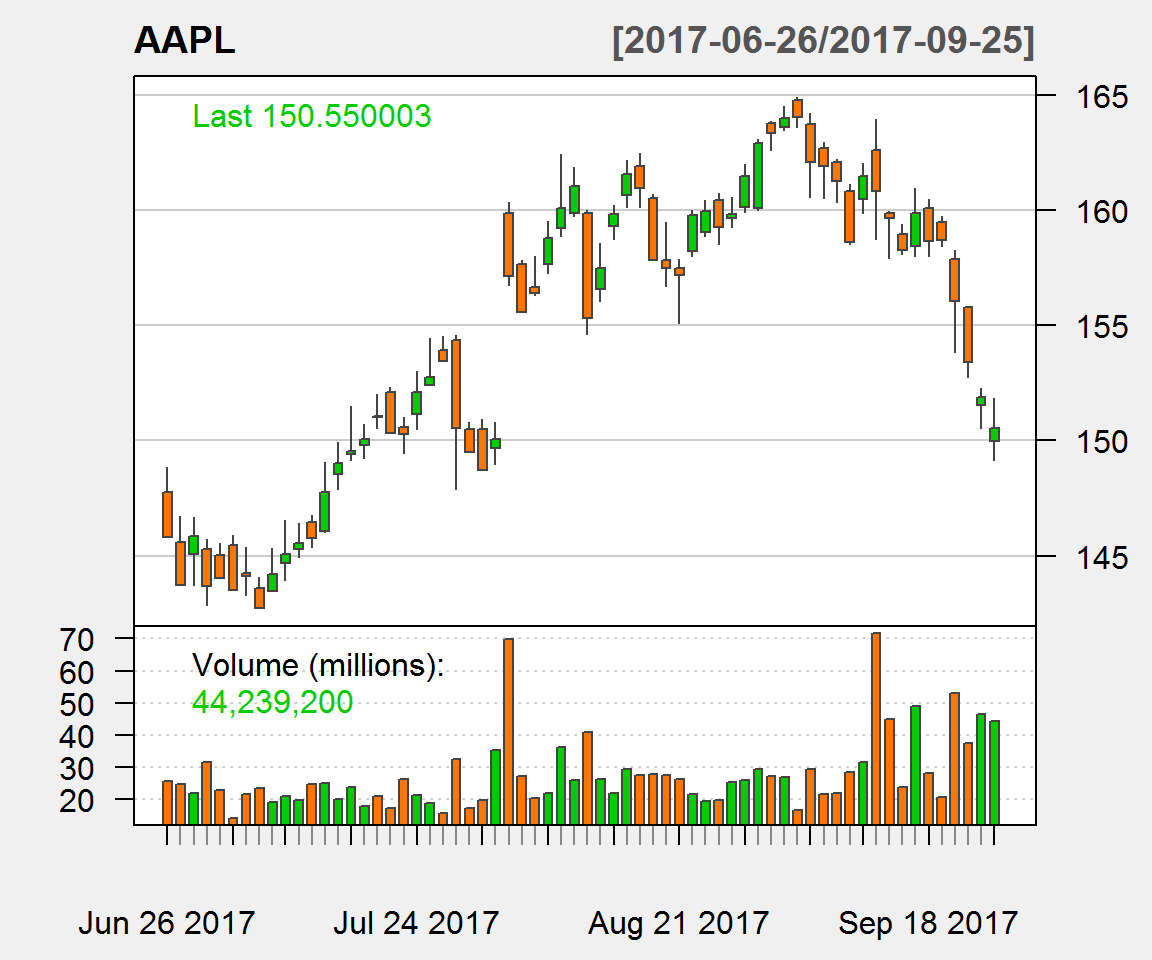
\includegraphics{ds_files/figure-latex/candleAAPL-1} 

}

\caption{Candlestick chart for Apple's stock price for the last three months.}\label{fig:candleAAPL}
\end{figure}

Using the price contained in the object we downloaded (i.e.
\texttt{AAPL}), we can compute Apple's arithmetic returns which are
defined as follows

\begin{equation}
  R_t = \frac{S_t - S_{t-1}}{S_{t-1}},
    \label{eq:returns}
\end{equation}

where \(R_t\) are the returns at time \emph{t} and \(S_t\) is the stock
price. This is implemented in the function \texttt{ClCl()} within the
\texttt{quantmod} package. For example, we can create a vector of
returns as follows

\begin{Shaded}
\begin{Highlighting}[]
\NormalTok{AAPL_returns <-}\StringTok{ }\KeywordTok{na.omit}\NormalTok{(}\KeywordTok{ClCl}\NormalTok{(AAPL))}
\end{Highlighting}
\end{Shaded}

where \texttt{na.omit()} is used to remove missing values in the stock
prices vector since, if we have \(n+1\) stock prices, we will only have
\(n\) returns and therefore the first return cannot be computed. We can
now compute the mean and median of the returns over the considered
period.

\begin{Shaded}
\begin{Highlighting}[]
\KeywordTok{mean}\NormalTok{(AAPL_returns)}
\end{Highlighting}
\end{Shaded}

\begin{verbatim}
## [1] 0.003111851
\end{verbatim}

\begin{Shaded}
\begin{Highlighting}[]
\KeywordTok{median}\NormalTok{(AAPL_returns)}
\end{Highlighting}
\end{Shaded}

\begin{verbatim}
## [1] 0.00258233
\end{verbatim}

However, a statistic that is of particular interest to financial
operators is the Excess Kurtosis which, for a random variable that we
denote as \(X\), can be defined as

\begin{equation}
  \text{Kurt} = \frac{{\mathbb{E}}\left[\left(X - \mathbb{E}[X]\right)^4\right]}{\left({\mathbb{E}}\left[\left(X - \mathbb{E}[X]\right)^2\right]\right)^2} - 3.
\end{equation}

The reason for defining this statistic as \emph{Excess} Kurtosis lies in
the fact that the standardized kurtosis is compared to that of a
Gaussian distribution (whose kurtosis is equal to 3) which has
exponentially decaying tails. Consequently, if the Excess Kurtosis is
positive, this implies that the distribution has heavier tails than a
Gaussian and therefore has higher probabilities of extreme events
occurring. To understand why the Excess Kurtosis is equal to 0 for a
Gaussian distribution click on the button below:

Excess Kurtosis Derivation

\hypertarget{hideclass1}{}
\BeginKnitrBlock{rmdnote}
Assuming \(X\) to be Gaussian, we have
\(X \sim \mathcal{N}(\mu, \sigma^2)\). Then, we define \(Z\) as
\(Z \sim \mathcal{N}(0,1)\) and \(Y\) as \(Y = Z^2 \sim \chi^2_1\).
Remember that a random variable following a \(\chi^2_1\) distribution
has the following properties: \(\text{Var}[Y] = 2\) and
\(\mathbb{E}[Y] = 1\). Using these definitions and properties, we
obtain:

\begin{equation}
  \begin{aligned}
\text{Kurt}  &= \frac{{\mathbb{E}}\left[\left(X - \mathbb{E}[X]\right)^4\right]}{\left({\mathbb{E}}\left[\left(X - \mathbb{E}[X]\right)^2\right]\right)^2} - 3 = \frac{{\mathbb{E}}\left[\left(X - \mathbb{E}[X]\right)^4\right]}{\left[\text{Var} \left(X\right)\right]^2} - 3 = \frac{{\mathbb{E}}\left[\left(X - \mathbb{E}[X]\right)^4\right]}{\sigma^4}  - 3\\
&= {\mathbb{E}}\left[\left(\frac{X - \mathbb{E}[X]}{\sigma}\right)^4\right] - 3 = \mathbb{E}\left[Z^4\right] - 3 = \text{Var}[Z^2] + \mathbb{E}^2\left[Z^2\right]  - 3\\
&= \text{Var}[Y] + \mathbb{E}^2\left[Y\right]  - 3 = 0.
  \end{aligned}
\end{equation}

This implies that the theoretical value of the excess Kurtosis for a
normally distributed random variable is \(0\).
\EndKnitrBlock{rmdnote}

\newline

Given this statistic, it is useful to compute this on the observed data
and for this purpose a common estimator of the excess Kurtosis is

\begin{equation}
  k = \frac{\frac{1}{n} \sum_{t = 1}^{n} \left(R_t -\bar{R}\right)^4}{\left(\frac{1}{n} \sum_{t = 1}^{n} \left(R_t -\bar{R}\right)^2 \right)^2} - 3,
\end{equation}

where \(\bar{R}\) denotes the sample average of the returns, i.e.

\begin{equation*}
  \bar{R} = \frac{1}{n} \sum_{i = 1}^n R_i.
\end{equation*}

In R, this can simply be done as follows:

\begin{Shaded}
\begin{Highlighting}[]
\NormalTok{mu <-}\StringTok{ }\KeywordTok{mean}\NormalTok{(AAPL_returns)}
\NormalTok{(k <-}\StringTok{ }\KeywordTok{mean}\NormalTok{((AAPL_returns }\OperatorTok{-}\StringTok{ }\NormalTok{mu)}\OperatorTok{^}\DecValTok{4}\NormalTok{)}\OperatorTok{/}\NormalTok{(}\KeywordTok{mean}\NormalTok{((AAPL_returns }\OperatorTok{-}\StringTok{ }\NormalTok{mu)}\OperatorTok{^}\DecValTok{2}\NormalTok{))}\OperatorTok{^}\DecValTok{2} \OperatorTok{-}\StringTok{ }\DecValTok{3}\NormalTok{)}
\end{Highlighting}
\end{Shaded}

\begin{verbatim}
## [1] 3.665572
\end{verbatim}

Therefore, we observe an estimated Excess Kurtosis of 3.67 which is
quite high and tends to indicate that the returns have heavier tails
than the normal distribution. In Chapter @ref(\#control), we will
revisit this example and investigate if there is \textbf{enough
evidence} to conclude that Apple's stock has Excess Kurtosis larger than
zero.

\section{Matrices}\label{matrices}

Matrices are a common data structure in R which have two dimensions to
store multiple vectors of the same length combined as a unified object.
The \texttt{matrix()} function can be used to create a matrix from a
vector:

\begin{Shaded}
\begin{Highlighting}[]
\NormalTok{(mat <-}\StringTok{ }\KeywordTok{matrix}\NormalTok{(}\DecValTok{1}\OperatorTok{:}\DecValTok{12}\NormalTok{, }\DataTypeTok{ncol =} \DecValTok{4}\NormalTok{,  }\DataTypeTok{nrow =} \DecValTok{3}\NormalTok{))}
\end{Highlighting}
\end{Shaded}

\begin{verbatim}
##      [,1] [,2] [,3] [,4]
## [1,]    1    4    7   10
## [2,]    2    5    8   11
## [3,]    3    6    9   12
\end{verbatim}

Notice that the first argument to the function is a vector (in this case
the sequence 1 to 12) which is then transformed into a matrix with four
columns (\texttt{ncol\ =\ 4}) and three rows (\texttt{nrow\ =\ 3}).

\BeginKnitrBlock{rmdtip}
By default, the vectors are transformed into matrices by placing the
elements by column (i.e.~top to the bottom of ech column in sequence
until all columns are full). If you wish to fill the matrix by row, all
you need to do is specify the argument \texttt{byrow\ =\ T}.
\EndKnitrBlock{rmdtip}

\begin{Shaded}
\begin{Highlighting}[]
\CommentTok{# Compare with the matrix above}
\KeywordTok{matrix}\NormalTok{(}\DecValTok{1}\OperatorTok{:}\DecValTok{12}\NormalTok{, }\DataTypeTok{ncol =} \DecValTok{4}\NormalTok{,  }\DataTypeTok{nrow =} \DecValTok{3}\NormalTok{, }\DataTypeTok{byrow =}\NormalTok{ T)}
\end{Highlighting}
\end{Shaded}

\begin{verbatim}
##      [,1] [,2] [,3] [,4]
## [1,]    1    2    3    4
## [2,]    5    6    7    8
## [3,]    9   10   11   12
\end{verbatim}

\BeginKnitrBlock{rmdwarning}
Usually the length of the vector (i.e.~number of elements in the vector)
is the result of the multiplication between the number of columns and
number of rows. What happens if the vector has fewer elements for the
same matrix dimension? What happens if the vector has more elements?
\EndKnitrBlock{rmdwarning}

It is often the case that we already have equi-dimensional vectors
available and we wish to bundle them together as matrix. In these cases,
two useful functions are \texttt{cbind()} to combine vectors as vertical
\textbf{c}olumns side-by-side, and \texttt{rbind()} to combine vectors
as horizontal \textbf{r}ows. An example of \texttt{cbind()} is shown
here:

\begin{Shaded}
\begin{Highlighting}[]
\NormalTok{players <-}\StringTok{ }\KeywordTok{c}\NormalTok{(}\StringTok{"Andy Murray"}\NormalTok{, }\StringTok{"Rafael Nadal"}\NormalTok{, }\StringTok{"Stan Wawrinka"}\NormalTok{, }
             \StringTok{"Novak Djokovic"}\NormalTok{, }\StringTok{"Roger Federer"}\NormalTok{)}
\NormalTok{grand_slam_win <-}\StringTok{ }\KeywordTok{c}\NormalTok{(}\DecValTok{9}\NormalTok{, }\DecValTok{15}\NormalTok{, }\DecValTok{5}\NormalTok{, }\DecValTok{12}\NormalTok{, }\DecValTok{18}\NormalTok{)}
\NormalTok{win_percentage <-}\StringTok{ }\KeywordTok{c}\NormalTok{(}\FloatTok{78.07}\NormalTok{, }\FloatTok{82.48}\NormalTok{, }\FloatTok{63.96}\NormalTok{, }\FloatTok{82.77}\NormalTok{, }\FloatTok{81.80}\NormalTok{)}
\NormalTok{(mat <-}\StringTok{ }\KeywordTok{cbind}\NormalTok{(grand_slam_win, win_percentage))}
\end{Highlighting}
\end{Shaded}

\begin{verbatim}
##      grand_slam_win win_percentage
## [1,]              9          78.07
## [2,]             15          82.48
## [3,]              5          63.96
## [4,]             12          82.77
## [5,]             18          81.80
\end{verbatim}

The result in this case is a \(5 \times 2\) matrix (with
\texttt{rbind()} it would have been a \(2 \times 5\) matrix). Once the
matrix is defined, we can assign names to its rows and columns by using
\texttt{rownames()} and \texttt{colnames()}, respectively. Of course,
the number of names must match the corresponding matrix dimension. In
the following example, each row corresponds to a specific player
(thereby using the \texttt{players} vector) and each column corresponds
to a specific statistic of the players.

\begin{Shaded}
\begin{Highlighting}[]
\KeywordTok{rownames}\NormalTok{(mat) <-}\StringTok{ }\NormalTok{players}
\KeywordTok{colnames}\NormalTok{(mat) <-}\StringTok{ }\KeywordTok{c}\NormalTok{(}\StringTok{"GS win"}\NormalTok{, }\StringTok{"Win rate"}\NormalTok{)}
\NormalTok{mat}
\end{Highlighting}
\end{Shaded}

\begin{verbatim}
##                GS win Win rate
## Andy Murray         9    78.07
## Rafael Nadal       15    82.48
## Stan Wawrinka       5    63.96
## Novak Djokovic     12    82.77
## Roger Federer      18    81.80
\end{verbatim}

\subsection{Subsetting}\label{subsetting-1}

As with vectors, it is possible to subset the elements of a matrix.
Since matrices are two-dimensional data structures, it is necessary to
specify the position of the elements of interest in both dimensions. For
this purpose we can use \texttt{{[}\ ,\ {]}} immediately following the
named matrix. Note the use of \texttt{,} within the square brackets in
order to specify both row and column position of desired elements within
the matrix (e.g. \texttt{matrixName{[}row,\ column{]}}). Consider the
following examples:

\begin{Shaded}
\begin{Highlighting}[]
\CommentTok{# Subset players "Stan Wawrinka" and "Roger Federer" in matrix named "mat"}
\NormalTok{mat[}\KeywordTok{c}\NormalTok{(}\StringTok{"Stan Wawrinka"}\NormalTok{, }\StringTok{"Roger Federer"}\NormalTok{), ]}
\end{Highlighting}
\end{Shaded}

\begin{verbatim}
##               GS win Win rate
## Stan Wawrinka      5    63.96
## Roger Federer     18    81.80
\end{verbatim}

\begin{Shaded}
\begin{Highlighting}[]
\CommentTok{# Subset includes row 1 and 3 for all columns }
\NormalTok{mat[}\KeywordTok{c}\NormalTok{(}\DecValTok{1}\NormalTok{, }\DecValTok{3}\NormalTok{), ]}
\end{Highlighting}
\end{Shaded}

\begin{verbatim}
##               GS win Win rate
## Andy Murray        9    78.07
## Stan Wawrinka      5    63.96
\end{verbatim}

\begin{Shaded}
\begin{Highlighting}[]
\CommentTok{# Subset includes all rows for column 2  }
\NormalTok{mat[ , }\DecValTok{2}\NormalTok{]}
\end{Highlighting}
\end{Shaded}

\begin{verbatim}
##    Andy Murray   Rafael Nadal  Stan Wawrinka Novak Djokovic  Roger Federer 
##          78.07          82.48          63.96          82.77          81.80
\end{verbatim}

\begin{Shaded}
\begin{Highlighting}[]
\CommentTok{# Subset includes rows 1, 2, & 3 for column 1  }
\NormalTok{mat[}\DecValTok{1}\OperatorTok{:}\DecValTok{3}\NormalTok{, }\DecValTok{1}\NormalTok{]}
\end{Highlighting}
\end{Shaded}

\begin{verbatim}
##   Andy Murray  Rafael Nadal Stan Wawrinka 
##             9            15             5
\end{verbatim}

It can be noticed that, when a space is left blank before or after the
comma, this means that respectively all the rows or all the columns are
considered.

\subsection{Matrix Operators in R}\label{matrix-operators-in-r}

As with vectors, there are some useful functions that can be used with
matrices. A first example is the function \texttt{dim()} that allows to
determine the dimension of a matrix. For example, consider the following
\(4 \times 2\) matrix

\begin{equation*}
\mathbf{A} = \left[
\begin{matrix}
1 & 5\\
2 & 6\\
3 & 7\\
4 & 8
\end{matrix}
\right]
\end{equation*}

which can be created in R as follows:

\begin{Shaded}
\begin{Highlighting}[]
\NormalTok{(A <-}\StringTok{ }\KeywordTok{matrix}\NormalTok{(}\DecValTok{1}\OperatorTok{:}\DecValTok{8}\NormalTok{, }\DecValTok{4}\NormalTok{, }\DecValTok{2}\NormalTok{))}
\end{Highlighting}
\end{Shaded}

\begin{verbatim}
##      [,1] [,2]
## [1,]    1    5
## [2,]    2    6
## [3,]    3    7
## [4,]    4    8
\end{verbatim}

Therefore, we expect \texttt{dim(A)} to return the vector
\texttt{c(4,\ 2)}. Indeed, we have

\begin{Shaded}
\begin{Highlighting}[]
\KeywordTok{dim}\NormalTok{(A)}
\end{Highlighting}
\end{Shaded}

\begin{verbatim}
## [1] 4 2
\end{verbatim}

Next, we consider the function \texttt{t()} that allows transpose a
matrix. For example, \(\mathbf{A}^T\) is equal to:

\begin{equation*}
\mathbf{A}^T = \left[
\begin{matrix}
1 & 2 & 3 & 4\\
5 & 6 & 7 & 8
\end{matrix}
\right],
\end{equation*}

which is a \(2 \times 4\) matrix. In R, we achieve this as follows

\begin{Shaded}
\begin{Highlighting}[]
\NormalTok{(At <-}\StringTok{ }\KeywordTok{t}\NormalTok{(A))}
\end{Highlighting}
\end{Shaded}

\begin{verbatim}
##      [,1] [,2] [,3] [,4]
## [1,]    1    2    3    4
## [2,]    5    6    7    8
\end{verbatim}

\begin{Shaded}
\begin{Highlighting}[]
\KeywordTok{dim}\NormalTok{(At)}
\end{Highlighting}
\end{Shaded}

\begin{verbatim}
## [1] 2 4
\end{verbatim}

Aside from playing with matrix dimensions, matrix algebraic operations
have specific commands. For example, the operator \texttt{\%*\%} is used
in R to denote matrix multiplication while, as opposed to scalar
objects, the regular product operator \texttt{*} performs the element by
element product (or Hadamard product) when applied to matrices. For
example, consider the following matrix product:

\begin{equation*}
  \mathbf{B} = \mathbf{A}^T \mathbf{A} =   \left[
\begin{matrix}
30 & 70\\
70 & 174
\end{matrix}
\right],
\end{equation*}

which can be done in R as follows:

\begin{Shaded}
\begin{Highlighting}[]
\NormalTok{(B <-}\StringTok{ }\NormalTok{At }\OperatorTok\StringTok{ }\NormalTok{A)}
\end{Highlighting}
\end{Shaded}

\begin{verbatim}
##      [,1] [,2]
## [1,]   30   70
## [2,]   70  174
\end{verbatim}

Other common matrix operations include finding the determinant of a
matrix and finding its inverse. These are often used, for example, when
computing the likelihood function for a variable following a Gaussian
distribution or when simulating time series or spatial data. The
functions that perform these operations are \texttt{det()} and
\texttt{solve()} that respectively find the determinant and the inverse
of a matrix (which necessarily has to be square). The function
\texttt{det()} can be used to compute the determinant of a square
matrix. In the case of a \(2 \times 2\) matrix, there exists a simple
solution for the determinant which is

\begin{equation*}
\text{det} \left( \mathbf{D} \right) = \text{det} \left( \left[
\begin{matrix}
d_1 & d_2\\
d_3 & d_4
\end{matrix}
\right] \right) = d_1 d_4 - d_2 d_3.
\end{equation*}

Consider the matrix \(\mathbf{B}\), we have

\begin{equation*}
  \text{det} \left( \mathbf{B}\right) = 30 \cdot 174 - 70^2 = 320.
\end{equation*}

In R, we can simply do

\begin{Shaded}
\begin{Highlighting}[]
\KeywordTok{det}\NormalTok{(B)}
\end{Highlighting}
\end{Shaded}

\begin{verbatim}
## [1] 320
\end{verbatim}

The function \texttt{solve()} is also an important function when working
with matrices as it allows to inverse a matrix. It is worth remembering
that a square matrix that is not invertible (i.e. \(\mathbf{A}^{-1}\)
doesn't exist) is called \emph{singular} and the determinant offers a
way to ``check'' if this is the case for a given matrix. Indeed, a
square matrix is singular if and only if its determinant is 0.
Therefore, in the case of \(\mathbf{B}\), we should be able to compute
its inverse. As for the determinant, there exists a formula to compute
the inverse of \(2 \times 2\) matrices, i.e.

\begin{equation*}
 \mathbf{D}^{-1} = \left[
\begin{matrix}
d_1 & d_2\\
d_3 & d_4
\end{matrix}
\right]^{-1} = \frac{1}{\text{det}\left( \mathbf{D} \right)} \left[
\begin{matrix}
\phantom{-}d_4 & -d_2\\
-d_3 & \phantom{-}d_1
\end{matrix}
\right].
\end{equation*}

Considering the matrix \(\mathbf{B}\), we obtain

\begin{equation*}
 \mathbf{B}^{-1} = \left[
\begin{matrix}
30 & 70\\
70 & 174
\end{matrix}
\right]^{-1} = \frac{1}{320}\left[
\begin{matrix}
  \phantom{-}174 & -70\\
-70 & \phantom{-}30
\end{matrix}
\right] = \left[
\begin{matrix}
  \phantom{-}0.54375 & -0.21875\\
-0.21875 & \phantom{-}0.09375
\end{matrix}
\right] 
\end{equation*}

\begin{Shaded}
\begin{Highlighting}[]
\NormalTok{(B_inv <-}\StringTok{ }\KeywordTok{solve}\NormalTok{(B))}
\end{Highlighting}
\end{Shaded}

\begin{verbatim}
##          [,1]     [,2]
## [1,]  0.54375 -0.21875
## [2,] -0.21875  0.09375
\end{verbatim}

Finally, we can verify that

\begin{equation*}
\mathbf{G} = \mathbf{B} \mathbf{B}^{-1},
\end{equation*}

should be equal to the identity matrix,

\begin{Shaded}
\begin{Highlighting}[]
\NormalTok{(G <-}\StringTok{ }\NormalTok{B }\OperatorTok\StringTok{ }\NormalTok{B_inv)}
\end{Highlighting}
\end{Shaded}

\begin{verbatim}
##      [,1]          [,2]
## [1,]    1 -8.881784e-16
## [2,]    0  1.000000e+00
\end{verbatim}

The result is of course extremely close but \(\mathbf{G}\) is not
exactly equal to the identity matrix due to rounding and other numerical
errors.

Another function of interest is the function \texttt{diag()} that can be
used to extract the diagonal of a matrix. For example, we have

\begin{equation*}
\text{diag} \left( \mathbf{B} \right) = \left[30 \;\; 174\right],
\end{equation*}

which can be done in R as follows:

\begin{Shaded}
\begin{Highlighting}[]
\KeywordTok{diag}\NormalTok{(B)}
\end{Highlighting}
\end{Shaded}

\begin{verbatim}
## [1]  30 174
\end{verbatim}

Therefore, the function \texttt{diag()} computes the trace of matrix
(i.e.~the sum of the diagonal elements). For example,

\begin{equation*}
\text{tr} \left( \mathbf{B} \right) = 204,
\end{equation*}

or in R:

\begin{Shaded}
\begin{Highlighting}[]
\KeywordTok{sum}\NormalTok{(}\KeywordTok{diag}\NormalTok{(B))}
\end{Highlighting}
\end{Shaded}

\begin{verbatim}
## [1] 204
\end{verbatim}

Another use of the function \texttt{diag()} is to create diagonal
matrices. Indeed, if the argument of this function is a vector, its
behavior is the following:

\begin{equation*}
  \text{diag} \left(\left[a_1 \;\; a_2 \;\; \cdots \;\; a_n\right]\right) = \left[
\begin{matrix}
a_1     & 0       & \cdots & 0  \\
0       & a_2     & \cdots & 0  \\
\vdots  & \vdots  & \ddots       & \vdots    \\
0       & 0       &   \cdots     & a_n
\end{matrix}
\right].
\end{equation*}

Therefore, this provides a simple way of creating an identity matrix by
combining the functions \texttt{diag()} and \texttt{rep()} (discussed in
the previous section) as follows:

\begin{Shaded}
\begin{Highlighting}[]
\NormalTok{n <-}\StringTok{ }\DecValTok{4}
\NormalTok{(ident <-}\StringTok{ }\KeywordTok{diag}\NormalTok{(}\KeywordTok{rep}\NormalTok{(}\DecValTok{1}\NormalTok{, n)))}
\end{Highlighting}
\end{Shaded}

\begin{verbatim}
##      [,1] [,2] [,3] [,4]
## [1,]    1    0    0    0
## [2,]    0    1    0    0
## [3,]    0    0    1    0
## [4,]    0    0    0    1
\end{verbatim}

\subsection{Example: Summary Statistics with Matrix
Notation}\label{example-summary-statistics-with-matrix-notation}

A simple example of the operations we discussed in the previous section
is given by many common statistics that can be re-expressed using matrix
notation. As an example, we will consider three common statistics that
are the sample mean, variance and covariance. Let us consider the
following two samples of size \(n\)

\begin{equation*}
  \begin{aligned}
    \mathbf{x} &= \left[x_1 \;\; x_2 \; \;\cdots \;\; x_n\right]^T\\
    \mathbf{y} &= \left[y_1 \;\;\; y_2 \; \;\;\cdots \;\;\; y_n\right]^T.
  \end{aligned}
\end{equation*}

The sample mean of \(\mathbf{x}\) is

\begin{equation*}
  \bar{x} = \frac{1}{n} \sum_{i = 1}^{n} x_i,
\end{equation*}

and its sample variance is

\begin{equation*}
  s_x^2 = \frac{1}{n} \sum_{i = 1}^n \left(x_i - \bar{x}\right)^2.
\end{equation*}

The sample covariance between \(\mathbf{x}\) and \(\mathbf{y}\) is

\begin{equation*}
  s_{x,y} = \frac{1}{n} \sum_{i = 1}^n \left(X_i - \bar{x}\right) \left(Y_i - \bar{y}\right),
\end{equation*}

where \(\bar{y}\) denotes the sample mean of \(\mathbf{y}\).

Consider the sample mean, this statistic can be expressed in matrix
notation as follows

\begin{equation*}
  \bar{x} = \frac{1}{n} \sum_{i = 1}^{n} x_i =  \frac{1}{n} \mathbf{x}^T \mathbf{1},
\end{equation*}

where \(\mathbf{1}\) is a column vector of \(n\) ones.

\begin{equation*}
  \begin{aligned}
    s_x^2 &= \frac{1}{n} \sum_{i = 1}^n \left(x_i - \bar{x}\right)^2 = \frac{1}{n} \sum_{i = 1}^n x_i^2 - \bar{x}^2 = \frac{1}{n} \mathbf{x}^T \mathbf{x} - \bar{x}^2\\
    &= \frac{1}{n} \mathbf{x}^T \mathbf{x} - \left(\frac{1}{n} \mathbf{x}^T \mathbf{1}\right)^2 = \frac{1}{n} \left(\mathbf{x}^T \mathbf{x} - \frac{1}{n} \mathbf{x}^T \mathbf{1} \mathbf{1}^T \mathbf{x}\right)\\
    &= \frac{1}{n}\mathbf{x}^T \left( \mathbf{I} - \frac{1}{n} \mathbf{1} \mathbf{1}^T \right) \mathbf{x} = \frac{1}{n}\mathbf{x}^T \mathbf{H} \mathbf{x},
  \end{aligned}
\end{equation*}

where \(\mathbf{H} = \mathbf{I} - \frac{1}{n} \mathbf{1} \mathbf{1}^T\).
This matrix is often called the \emph{centering} matrix. Similarly, for
the sample covariance we obtain

\begin{equation*}
  \begin{aligned}
    s_{x,y} &= \frac{1}{n} \sum_{i = 1}^n \left(x_i - \bar{x}\right) \left(y_i - \bar{y}\right) = \frac{1}{n}\mathbf{x}^T \mathbf{H} \mathbf{y}.
  \end{aligned}
\end{equation*}

In the code below we verify the validity of these results through a
simple simulated example where we compare the values of the three
statistics based on the different formulas discussed above.

\begin{Shaded}
\begin{Highlighting}[]
\CommentTok{# Sample size}
\NormalTok{n <-}\StringTok{ }\DecValTok{100}

\CommentTok{# Simulate random numbers from a zero mean normal distribution with}
\CommentTok{# variance equal to 4.}
\NormalTok{x <-}\StringTok{ }\KeywordTok{rnorm}\NormalTok{(n, }\DecValTok{0}\NormalTok{, }\KeywordTok{sqrt}\NormalTok{(}\DecValTok{4}\NormalTok{))}

\CommentTok{# Simulate random numbers from normal distribution with mean 3 and}
\CommentTok{# variance equal to 1.}
\NormalTok{y <-}\StringTok{ }\KeywordTok{rnorm}\NormalTok{(n, }\DecValTok{3}\NormalTok{, }\DecValTok{1}\NormalTok{)}

\CommentTok{# Note that x and y are independent.}

\CommentTok{# Sample mean}
\NormalTok{one <-}\StringTok{ }\KeywordTok{rep}\NormalTok{(}\DecValTok{1}\NormalTok{, n)}
\NormalTok{x_bar <-}\StringTok{ }\DecValTok{1}\OperatorTok{/}\NormalTok{n}\OperatorTok{*}\KeywordTok{sum}\NormalTok{(x)}
\NormalTok{x_bar_mat <-}\StringTok{ }\DecValTok{1}\OperatorTok{/}\NormalTok{n}\OperatorTok{*}\KeywordTok{t}\NormalTok{(x)}\OperatorTok\NormalTok{one}

\CommentTok{# Sample variance of x}
\NormalTok{H <-}\StringTok{ }\KeywordTok{diag}\NormalTok{(}\KeywordTok{rep}\NormalTok{(}\DecValTok{1}\NormalTok{, n)) }\OperatorTok{-}\StringTok{ }\DecValTok{1}\OperatorTok{/}\NormalTok{n }\OperatorTok{*}\StringTok{ }\NormalTok{one }\OperatorTok\StringTok{ }\KeywordTok{t}\NormalTok{(one)}
\NormalTok{s_x <-}\StringTok{ }\DecValTok{1}\OperatorTok{/}\NormalTok{n }\OperatorTok{*}\StringTok{ }\KeywordTok{sum}\NormalTok{((x }\OperatorTok{-}\StringTok{ }\NormalTok{x_bar)}\OperatorTok{^}\DecValTok{2}\NormalTok{)}
\NormalTok{s_x_mat <-}\StringTok{ }\DecValTok{1}\OperatorTok{/}\NormalTok{n}\OperatorTok{*}\KeywordTok{t}\NormalTok{(x) }\OperatorTok\StringTok{ }\NormalTok{H }\OperatorTok\StringTok{ }\NormalTok{x}

\CommentTok{# Sample covariance}
\NormalTok{y_bar <-}\StringTok{ }\DecValTok{1}\OperatorTok{/}\NormalTok{n}\OperatorTok{*}\KeywordTok{sum}\NormalTok{(y)}
\NormalTok{s_xy <-}\StringTok{ }\DecValTok{1}\OperatorTok{/}\NormalTok{n}\OperatorTok{*}\KeywordTok{sum}\NormalTok{((x }\OperatorTok{-}\StringTok{ }\NormalTok{x_bar)}\OperatorTok{*}\NormalTok{(y }\OperatorTok{-}\StringTok{ }\NormalTok{y_bar))}
\NormalTok{s_xy_mat <-}\StringTok{ }\DecValTok{1}\OperatorTok{/}\NormalTok{n}\OperatorTok{*}\KeywordTok{t}\NormalTok{(x) }\OperatorTok\StringTok{ }\NormalTok{H }\OperatorTok\StringTok{ }\NormalTok{y}
\end{Highlighting}
\end{Shaded}

To compare, let's construct a matrix of all the results that we
calculated.

\begin{Shaded}
\begin{Highlighting}[]
\NormalTok{cp_matrix <-}\StringTok{ }\KeywordTok{matrix}\NormalTok{(}\KeywordTok{c}\NormalTok{(x_bar, x_bar_mat, s_x, s_x_mat, s_xy, s_xy_mat), }\DataTypeTok{ncol =} \DecValTok{2}\NormalTok{, }\DataTypeTok{byrow =}\NormalTok{ T)}
\KeywordTok{row.names}\NormalTok{(cp_matrix) <-}\StringTok{ }\KeywordTok{c}\NormalTok{(}\StringTok{"Sample Mean"}\NormalTok{, }\StringTok{"Sample Variance"}\NormalTok{, }\StringTok{"Sample Covariance"}\NormalTok{)}
\KeywordTok{colnames}\NormalTok{(cp_matrix) <-}\StringTok{ }\KeywordTok{c}\NormalTok{(}\StringTok{"Scalar"}\NormalTok{, }\StringTok{"Matrix"}\NormalTok{)}
\NormalTok{cp_matrix}
\end{Highlighting}
\end{Shaded}

\begin{verbatim}
##                       Scalar     Matrix
## Sample Mean        0.1374096  0.1374096
## Sample Variance    4.4333314  4.4333314
## Sample Covariance -0.3624978 -0.3624978
\end{verbatim}

Therefore, using the previously obtained results we can construct the
following \emph{empirical} covariance matrix

\begin{equation} 
  \widehat{\text{Cov}}(X, Y) =  \left[
\begin{matrix}
s_x^2        & s_{x,y}    \\
s_{x,y}      & s_y^2
\end{matrix}
\right].
\end{equation}

In R, this can be done as

\begin{Shaded}
\begin{Highlighting}[]
\CommentTok{# Sample variance of y}
\NormalTok{s_y_mat <-}\StringTok{ }\DecValTok{1}\OperatorTok{/}\NormalTok{n}\OperatorTok{*}\KeywordTok{t}\NormalTok{(y) }\OperatorTok\StringTok{ }\NormalTok{H }\OperatorTok\StringTok{ }\NormalTok{y}

\CommentTok{# Covariance matrix}
\NormalTok{(V <-}\StringTok{ }\KeywordTok{matrix}\NormalTok{(}\KeywordTok{c}\NormalTok{(s_x_mat, s_xy_mat, s_xy_mat, s_y_mat), }\DecValTok{2}\NormalTok{, }\DecValTok{2}\NormalTok{))}
\end{Highlighting}
\end{Shaded}

\begin{verbatim}
##            [,1]       [,2]
## [1,]  4.4333314 -0.3624978
## [2,] -0.3624978  1.1356772
\end{verbatim}

This result can now be compared to

\begin{Shaded}
\begin{Highlighting}[]
\KeywordTok{cov}\NormalTok{(}\KeywordTok{cbind}\NormalTok{(x, y))}
\end{Highlighting}
\end{Shaded}

\begin{verbatim}
##            x          y
## x  4.4781125 -0.3661594
## y -0.3661594  1.1471486
\end{verbatim}

We can see that the results are slightly different from what we
expected. This is because the calculation of \texttt{cov()} within the
default R \texttt{stats} package is based on an unbiased estimator which
is not the one we used. To obtain the same result, we can go back to our
estimation by calculating via the below method

\begin{Shaded}
\begin{Highlighting}[]
\NormalTok{(n}\OperatorTok{-}\DecValTok{1}\NormalTok{)}\OperatorTok{/}\NormalTok{n}\OperatorTok{*}\KeywordTok{cov}\NormalTok{(}\KeywordTok{cbind}\NormalTok{(x, y))}
\end{Highlighting}
\end{Shaded}

\begin{verbatim}
##            x          y
## x  4.4333314 -0.3624978
## y -0.3624978  1.1356772
\end{verbatim}

\subsection{Example: Portfolio
Optimization}\label{example-portfolio-optimization}

Suppose that you are interested in investing your money in two stocks,
say Apple and Netflix. However, you are wondering how much of each stock
you should buy. To make it simple let us assume that you will invest
\(\omega W\) in Apple (AAPL) and \((1-\omega) W\) in Netflix (NFLX),
where \(W\) denotes the amount of money you would like to invest, and
\(\omega \in [0, \, 1]\) dictates the proportion allocated to each
investment. Let \(R_A\) and \(R_N\) denote, respectively, the daily
return (see Equation \eqref{eq:returns} if you don't remember what returns
are) of Apple and Netflix. To make things simple we assume that the
returns \(R_A\) and \(R_N\) are jointly normally distributed so we can
write

\[
\mathbf{R} \stackrel{iid}{\sim} \mathcal{N} \left(\boldsymbol{\mu}, \boldsymbol{\Sigma}\right),
\]

where

\[
\mathbf{R} = \left[
\begin{matrix}
 R_A\\
 R_N
\end{matrix} 
\right], \;\;\;\; \boldsymbol{\mu} = \left[
\begin{matrix}
 \mu_A\\
 \mu_N
\end{matrix} 
\right], \;\; \text{and}\;\; \boldsymbol{\Sigma} = \left[
\begin{matrix}
 \sigma_A^2 & \sigma_{AN}\\
 \sigma_{AN} & \sigma_N^2
\end{matrix} 
\right].
\]

Using these assumptions, the classical portfolio optimization problem,
which would allow you to determine a ``good'' value of \(\omega\), can
be stated as follows: Given our initial wealth \(W\), the investment
problem is to decide how much should be invested in our first asset
(Apple) and in our second asset (Netflix). As mentioned earlier, we
assume that \(\omega \in [0,\,1]\), implying that it is only possible to
buy the two assets (i.e. \emph{short positions} are not allowed).
Therefore, to solve our investment problem we must choose the value of
\(\omega\) which would maximize your personal \emph{utility}. Informally
speaking, the utility represents a measurement of the ``usefulness''
that is obtained from your investment. To consider a simple case, we
will assume that you are a particularly \emph{risk averse} individual
(i.e.~you are looking for an investment that is as sure and safe as
possible) and as such you want to pick the value of \(\omega\) providing
you with the smallest investment risk. We can then determine the optimal
value of \(\omega\) as follows. First, we construct a new random
variable, say \(Y\), which denotes the return of your portfolio. Since
you invest \(\omega W\) in Apple and \((1 - \omega) W\) in Netflix, it
is easy to see that

\[Y = \left[\omega R_A + (1 - \omega) R_N \right]W.\]

In general the risk and variance of an investment are two different
things but in our case we assume that the return \(\mathbf{R}\) is
normally distributed and in this case the variance can perfectly
characterize the risk of our investment. Therefore, we can define the
risk of our investment as the following function of \(\omega\)

\[f(\omega) = \text{Risk}(Y) = \text{Var} (Y) =  \left[\omega^2 \sigma_A^2 + (1 - \omega)^2 \sigma_N^2 + 2 \omega (1 - \omega) \sigma_{AN}\right]W^2.\]

The function \(f(\omega)\) is minimized for the value \(\omega^*\) which
is given by

\begin{equation}
  \omega^* = \frac{\sigma^2_N - \sigma_{AN}}{\sigma^2_A + \sigma^2_N - 2\sigma_{AN}}.
  \label{eq:omega}
\end{equation}

If you are interested in understanding how Equation \eqref{eq:omega} was
obtained, click on the button below:



Minimum Variance Portfolio Derivation

\hypertarget{hideclass2}{}
\BeginKnitrBlock{rmdnote}
To obtain \(\omega^*\) we first differentiate the function \(f(\omega)\)
with respect to \(\omega\), which gives

\begin{equation}
  \frac{\partial}{\partial \omega} \, f(\omega) = \left[2 \omega \sigma_A^2 - 2 (1 - \omega) \sigma_N^2 + 2  (1 - 2\omega) \sigma_{AN}\right]W^2
\end{equation}

Then, we define \(\omega^*\) as

\begin{equation}
  \omega^* \; : \frac{\partial}{\partial \omega} \, f(\omega) = 0.
\end{equation}

Therefore, we obtain

\begin{equation}
  \omega^* \left(\sigma_A^2 + \sigma_N^2 - 2 \sigma_{AN}\right) = \sigma_N^2 - \sigma_{AN},
\end{equation}

which simplifies to

\begin{equation}
  \omega^*  = \frac{\sigma_N^2 - \sigma_{AN}}{\sigma_A^2 + \sigma_N^2 - 2 \sigma_{AN}}. 
\end{equation}

Finally, we verify that our result is a minimum by considering the
second derivative, i.e.

\begin{equation}
  \frac{\partial^2}{\partial \omega^2} \, f(\omega) = 2W\left[\sigma_A^2 + \sigma_N^2 - 2\sigma_{AN} \sigma_{AN}\right].
\end{equation}

Since \(W\) is strictly positive, all that remains to conclude our
derivation is to verify that
\(\sigma_A^2 + \sigma_N^2 - 2\sigma_{AN} \sigma_{AN} \leq 0\). In fact,
this is a well known inequality which is a direct consequence of the
Tchebychev inequality. However, here is a simpler argument to understand
why this is the case. Indeed, it is obvious that
\(\text{Var}(R_A - R_N) \leq 0\) and we also have
\(\text{Var}(R_A - R_N) = \sigma_A^2 + \sigma_N^2 - 2\sigma_{AN}\).
Thus, we obtain

\[\text{Var}(R_A - R_N) = \sigma_A^2 + \sigma_N^2 - 2\sigma_{AN} \leq 0,\]

which verifies that our result is a minimum.
\EndKnitrBlock{rmdnote}

\newline

Using \eqref{eq:omega}, we obtain that the expected value and variance of
our investment are given by

\[
\begin{aligned}
\text{Expected Value Investment} &=\left[\omega^* \mu_A + (1 - \omega^*) \mu_N\right] W,\\
\text{Variance Investment} &=  \left[(\omega^*)^2 \sigma_A^2 + (1 - \omega^*)^2 \sigma_N^2 + 2 \omega^* (1 - \omega^*) \sigma_{AN}\right]W^2.
\end{aligned}
\]

In practice, the vector \(\boldsymbol{\mu}\) and the matrix
\(\boldsymbol{\Sigma}\) are unknown and must be estimated using
historical data. In the code below, we compute the optimal value of
\(\omega\) based on \eqref{eq:omega} by using the last five years of
historical data for the two stocks considered. For simplicity we set
\(W\) to one but note that \(W\) plays no role in determining
\(\omega^*\).

\begin{Shaded}
\begin{Highlighting}[]
\CommentTok{# Load quantmod}
\KeywordTok{library}\NormalTok{(quantmod)}

\CommentTok{# Download data}
\NormalTok{today <-}\StringTok{ }\KeywordTok{Sys.Date}\NormalTok{()}
\NormalTok{five_years_ago <-}\StringTok{ }\KeywordTok{seq}\NormalTok{(today, }\DataTypeTok{length =} \DecValTok{2}\NormalTok{, }\DataTypeTok{by =} \StringTok{"-5 year"}\NormalTok{)[}\DecValTok{2}\NormalTok{]}
\KeywordTok{getSymbols}\NormalTok{(}\StringTok{"AAPL"}\NormalTok{, }\DataTypeTok{from =}\NormalTok{ five_years_ago, }\DataTypeTok{to =}\NormalTok{ today)}
\KeywordTok{getSymbols}\NormalTok{(}\StringTok{"NFLX"}\NormalTok{, }\DataTypeTok{from =}\NormalTok{ five_years_ago, }\DataTypeTok{to =}\NormalTok{ today)}

\CommentTok{# Compute returns}
\NormalTok{Ra <-}\StringTok{ }\KeywordTok{na.omit}\NormalTok{(}\KeywordTok{ClCl}\NormalTok{(AAPL))}
\NormalTok{Rn <-}\StringTok{ }\KeywordTok{na.omit}\NormalTok{(}\KeywordTok{ClCl}\NormalTok{(NFLX)) }

\CommentTok{# Estimation of mu and Sigma}
\NormalTok{Sigma <-}\StringTok{ }\KeywordTok{cov}\NormalTok{(}\KeywordTok{cbind}\NormalTok{(Ra, Rn))}
\NormalTok{mu <-}\StringTok{ }\KeywordTok{c}\NormalTok{(}\KeywordTok{mean}\NormalTok{(Ra), }\KeywordTok{mean}\NormalTok{(Rn))}

\CommentTok{# Compute omega^*}
\NormalTok{omega_star <-}\StringTok{ }\NormalTok{(Sigma[}\DecValTok{2}\NormalTok{, }\DecValTok{2}\NormalTok{] }\OperatorTok{-}\StringTok{ }\NormalTok{Sigma[}\DecValTok{1}\NormalTok{, }\DecValTok{2}\NormalTok{])}\OperatorTok{/}\NormalTok{(Sigma[}\DecValTok{1}\NormalTok{, }\DecValTok{1}\NormalTok{] }\OperatorTok{+}\StringTok{ }\NormalTok{Sigma[}\DecValTok{2}\NormalTok{, }\DecValTok{2}\NormalTok{] }\OperatorTok{-}\StringTok{ }\DecValTok{2}\OperatorTok{*}\NormalTok{Sigma[}\DecValTok{1}\NormalTok{, }\DecValTok{2}\NormalTok{])}

\CommentTok{# Compute investment expected value and variance}
\NormalTok{mu_investment <-}\StringTok{ }\NormalTok{omega_star}\OperatorTok{*}\NormalTok{mu[}\DecValTok{1}\NormalTok{] }\OperatorTok{+}\StringTok{ }\NormalTok{(}\DecValTok{1} \OperatorTok{-}\StringTok{ }\NormalTok{omega_star)}\OperatorTok{*}\NormalTok{mu[}\DecValTok{2}\NormalTok{]}
\NormalTok{var_investment <-}\StringTok{ }\NormalTok{omega_star}\OperatorTok{^}\DecValTok{2}\OperatorTok{*}\NormalTok{Sigma[}\DecValTok{1}\NormalTok{,}\DecValTok{1}\NormalTok{] }\OperatorTok{+}\StringTok{ }\NormalTok{(}\DecValTok{1} \OperatorTok{-}\StringTok{ }\NormalTok{omega_star)}\OperatorTok{^}\DecValTok{2}\OperatorTok{*}\NormalTok{Sigma[}\DecValTok{2}\NormalTok{,}\DecValTok{2}\NormalTok{] }\OperatorTok{+}\StringTok{ }
\StringTok{  }\DecValTok{2}\OperatorTok{*}\NormalTok{omega_star}\OperatorTok{*}\NormalTok{(}\DecValTok{1} \OperatorTok{-}\StringTok{ }\NormalTok{omega_star)}\OperatorTok{*}\NormalTok{Sigma[}\DecValTok{1}\NormalTok{,}\DecValTok{2}\NormalTok{]}
\end{Highlighting}
\end{Shaded}

From this code, we obtain \(\omega^* \approx\) 85.63\%. In the table
below we compare the empirical expected values and variances of the
stocks as well as those of our investment:

\begin{Shaded}
\begin{Highlighting}[]
\NormalTok{investment_summary <-}\StringTok{ }\KeywordTok{matrix}\NormalTok{(}\OtherTok{NA}\NormalTok{, }\DecValTok{2}\NormalTok{, }\DecValTok{3}\NormalTok{)}
\KeywordTok{dimnames}\NormalTok{(investment_summary)[[}\DecValTok{1}\NormalTok{]] <-}\StringTok{ }\KeywordTok{c}\NormalTok{(}\StringTok{"Expected value"}\NormalTok{, }\StringTok{"Variance"}\NormalTok{)}
\KeywordTok{dimnames}\NormalTok{(investment_summary)[[}\DecValTok{2}\NormalTok{]] <-}\StringTok{ }\KeywordTok{c}\NormalTok{(}\StringTok{"Apple"}\NormalTok{, }\StringTok{"Netflix"}\NormalTok{, }\StringTok{"Investment"}\NormalTok{)}
\NormalTok{investment_summary[}\DecValTok{1}\NormalTok{, ] <-}\StringTok{ }\KeywordTok{c}\NormalTok{(mu, mu_investment)}
\NormalTok{investment_summary[}\DecValTok{2}\NormalTok{, ] <-}\StringTok{ }\KeywordTok{c}\NormalTok{(}\KeywordTok{diag}\NormalTok{(Sigma), var_investment)}
\NormalTok{knitr}\OperatorTok{::}\KeywordTok{kable}\NormalTok{(investment_summary)}
\end{Highlighting}
\end{Shaded}

\begin{table}

\caption{\label{tab:tableprtexample}Expected value and variance of stocks and our investment}
\centering
\begin{tabular}[t]{l|r|r|r}
\hline
  & Apple & Netflix & Investment\\
\hline
Expected value & 0.0010348 & 0.0020067 & 0.0011745\\
\hline
Variance & 0.0002010 & 0.0006991 & 0.0001865\\
\hline
\end{tabular}
\end{table}

In Table \ref{tab:tableprtexample} and the plot below we can observe
that Netflix has high risk and high return. Apple seems like a safer
investment in terms of risk but lower in expected return. Our portfolio
optimization investment, however, seems to be in a good area, meaning
that it has low risk and a return that is between the two stocks
mentioned above. Finally, we provide a graphical representation of the
obtained results in the figure below.

\subsection{NEED TO FIX THIS}\label{need-to-fix-this}

In the next chapter we will revisit this example where we will use new
programming tools to consider a more flexible solution to this
investment problem.

\section{Array}\label{array}

Arrays allow to construct \textbf{multidimensional} objects. Indeed,
vectors and matrices are respectively objects in one and two dimensions
while arrays can in be in an arbitrary \(n\) dimension. Essentially,
matrices are a special case of arrays which is only in two dimensions.
Matrices are commonly used in Statistics while arrays are much rarer but
nevertheless worth being aware of. To consider a simple using arrays we
will revisit an example presented in the previous section where we
constructed a matrix containing the number of Grand Slam won and the win
rate of the five players considered in Table \ref{tab:tennis}. This
matrix was constructed as follows:

\begin{Shaded}
\begin{Highlighting}[]
\NormalTok{players <-}\StringTok{ }\KeywordTok{c}\NormalTok{(}\StringTok{"Andy Murray"}\NormalTok{, }\StringTok{"Rafael Nadal"}\NormalTok{, }\StringTok{"Stan Wawrinka"}\NormalTok{, }
             \StringTok{"Novak Djokovic"}\NormalTok{, }\StringTok{"Roger Federer"}\NormalTok{)}
\NormalTok{grand_slam_win <-}\StringTok{ }\KeywordTok{c}\NormalTok{(}\DecValTok{9}\NormalTok{, }\DecValTok{15}\NormalTok{, }\DecValTok{5}\NormalTok{, }\DecValTok{12}\NormalTok{, }\DecValTok{18}\NormalTok{)}
\NormalTok{win_percentage <-}\StringTok{ }\KeywordTok{c}\NormalTok{(}\FloatTok{78.07}\NormalTok{, }\FloatTok{82.48}\NormalTok{, }\FloatTok{63.96}\NormalTok{, }\FloatTok{82.77}\NormalTok{, }\FloatTok{81.80}\NormalTok{)}
\NormalTok{mat <-}\StringTok{ }\KeywordTok{cbind}\NormalTok{(grand_slam_win, win_percentage)}
\KeywordTok{rownames}\NormalTok{(mat) <-}\StringTok{ }\NormalTok{players}
\KeywordTok{colnames}\NormalTok{(mat) <-}\StringTok{ }\KeywordTok{c}\NormalTok{(}\StringTok{"GS win"}\NormalTok{, }\StringTok{"Win rate"}\NormalTok{)}
\NormalTok{mat}
\end{Highlighting}
\end{Shaded}

\begin{verbatim}
##                GS win Win rate
## Andy Murray         9    78.07
## Rafael Nadal       15    82.48
## Stan Wawrinka       5    63.96
## Novak Djokovic     12    82.77
## Roger Federer      18    81.80
\end{verbatim}

The data used to construct this matrix we collected in mid-July 2017 and
suppose that we now would like to add to this existing the object the
updated numbers from mid-September 2017. This can be done by
constructing an array as shown in the example below.

\begin{Shaded}
\begin{Highlighting}[]
\CommentTok{# Constuct "empty" array}
\NormalTok{my_array <-}\StringTok{ }\KeywordTok{array}\NormalTok{(}\OtherTok{NA}\NormalTok{, }\DataTypeTok{dim =} \KeywordTok{c}\NormalTok{(}\DecValTok{5}\NormalTok{, }\DecValTok{2}\NormalTok{, }\DecValTok{2}\NormalTok{))}
\KeywordTok{dimnames}\NormalTok{(my_array)[[}\DecValTok{1}\NormalTok{]] <-}\StringTok{ }\NormalTok{players}
\KeywordTok{dimnames}\NormalTok{(my_array)[[}\DecValTok{2}\NormalTok{]] <-}\StringTok{ }\KeywordTok{c}\NormalTok{(}\StringTok{"GS win"}\NormalTok{, }\StringTok{"Win rate"}\NormalTok{)}
\KeywordTok{dimnames}\NormalTok{(my_array)[[}\DecValTok{3}\NormalTok{]] <-}\StringTok{ }\KeywordTok{c}\NormalTok{(}\StringTok{"07-15-2017"}\NormalTok{, }\StringTok{"09-13-2017"}\NormalTok{)}

\CommentTok{# Construct matrix}
\NormalTok{my_array[,,}\DecValTok{1}\NormalTok{] <-}\StringTok{ }\NormalTok{mat}
\NormalTok{my_array[,,}\DecValTok{2}\NormalTok{] <-}\StringTok{ }\KeywordTok{cbind}\NormalTok{(}\KeywordTok{c}\NormalTok{(}\DecValTok{9}\NormalTok{, }\DecValTok{16}\NormalTok{, }\DecValTok{5}\NormalTok{, }\DecValTok{12}\NormalTok{, }\DecValTok{19}\NormalTok{), }
                       \KeywordTok{c}\NormalTok{(}\FloatTok{78.07}\NormalTok{, }\FloatTok{82.49}\NormalTok{, }\FloatTok{63.96}\NormalTok{, }\FloatTok{82.77}\NormalTok{, }\FloatTok{81.80}\NormalTok{))}
\NormalTok{my_array}
\end{Highlighting}
\end{Shaded}

\begin{verbatim}
## , , 07-15-2017
## 
##                GS win Win rate
## Andy Murray         9    78.07
## Rafael Nadal       15    82.48
## Stan Wawrinka       5    63.96
## Novak Djokovic     12    82.77
## Roger Federer      18    81.80
## 
## , , 09-13-2017
## 
##                GS win Win rate
## Andy Murray         9    78.07
## Rafael Nadal       16    82.49
## Stan Wawrinka       5    63.96
## Novak Djokovic     12    82.77
## Roger Federer      19    81.80
\end{verbatim}

Like what we experimented with matrices, we can extract and manipulate
information.

\begin{Shaded}
\begin{Highlighting}[]
\KeywordTok{length}\NormalTok{(my_array)    }\CommentTok{# length is 20, i.e. 5x2x2 = 20}
\end{Highlighting}
\end{Shaded}

\begin{verbatim}
## [1] 20
\end{verbatim}

\begin{Shaded}
\begin{Highlighting}[]
\KeywordTok{dim}\NormalTok{(my_array)       }\CommentTok{# dimensions are 5x2x2}
\end{Highlighting}
\end{Shaded}

\begin{verbatim}
## [1] 5 2 2
\end{verbatim}

\begin{Shaded}
\begin{Highlighting}[]
\KeywordTok{is.array}\NormalTok{(my_array)  }\CommentTok{# yes it is an array!}
\end{Highlighting}
\end{Shaded}

\begin{verbatim}
## [1] TRUE
\end{verbatim}

Subsetting the elements of an array works similarly to what we already
discussed with matrices. Below are a few examples:

\begin{Shaded}
\begin{Highlighting}[]
\NormalTok{my_array[,,}\DecValTok{1}\NormalTok{]}
\end{Highlighting}
\end{Shaded}

\begin{verbatim}
##                GS win Win rate
## Andy Murray         9    78.07
## Rafael Nadal       15    82.48
## Stan Wawrinka       5    63.96
## Novak Djokovic     12    82.77
## Roger Federer      18    81.80
\end{verbatim}

\begin{Shaded}
\begin{Highlighting}[]
\NormalTok{my_array[}\DecValTok{1}\NormalTok{,,}\DecValTok{2}\NormalTok{]}
\end{Highlighting}
\end{Shaded}

\begin{verbatim}
##   GS win Win rate 
##     9.00    78.07
\end{verbatim}

\begin{Shaded}
\begin{Highlighting}[]
\NormalTok{my_array[,}\DecValTok{1}\NormalTok{,]}
\end{Highlighting}
\end{Shaded}

\begin{verbatim}
##                07-15-2017 09-13-2017
## Andy Murray             9          9
## Rafael Nadal           15         16
## Stan Wawrinka           5          5
## Novak Djokovic         12         12
## Roger Federer          18         19
\end{verbatim}

Finally, we can assess if some our five won any Grand Slam between
mid-July and mid-September 2017 by using the code below:

\begin{Shaded}
\begin{Highlighting}[]
\NormalTok{players[my_array[,}\DecValTok{1}\NormalTok{,}\DecValTok{2}\NormalTok{] }\OperatorTok{>}\StringTok{ }\NormalTok{my_array[,}\DecValTok{1}\NormalTok{,}\DecValTok{1}\NormalTok{]]}
\end{Highlighting}
\end{Shaded}

\begin{verbatim}
## [1] "Rafael Nadal"  "Roger Federer"
\end{verbatim}

\section{List}\label{list}

A list is one of the commonly used \textbf{heterogeneous} data
structures, which depicts a generic ``vector'' containing other object
types. For example, we can create a list containing numeric character
and logical vectors as well as matrices. Here we can create a list that
contains different element types. (numeric, character, logical, matrix)

\begin{Shaded}
\begin{Highlighting}[]
\CommentTok{# List elements}
\NormalTok{num_vec <-}\StringTok{ }\KeywordTok{c}\NormalTok{(}\DecValTok{188}\NormalTok{, }\DecValTok{140}\NormalTok{)}
\NormalTok{char_vec <-}\StringTok{ }\KeywordTok{c}\NormalTok{(}\StringTok{"Height"}\NormalTok{, }\StringTok{"Weight"}\NormalTok{, }\StringTok{"Length"}\NormalTok{)}
\NormalTok{logic_vec <-}\StringTok{ }\KeywordTok{rep}\NormalTok{(}\OtherTok{TRUE}\NormalTok{, }\DecValTok{8}\NormalTok{)}
\NormalTok{my_mat <-}\StringTok{ }\KeywordTok{matrix}\NormalTok{(}\DecValTok{0}\NormalTok{, }\DataTypeTok{nrow =} \DecValTok{5}\NormalTok{, }\DataTypeTok{ncol =} \DecValTok{5}\NormalTok{)}

\CommentTok{# List initialization }
\NormalTok{(my_list <-}\StringTok{ }\KeywordTok{list}\NormalTok{(num_vec, char_vec, logic_vec, my_mat))}
\end{Highlighting}
\end{Shaded}

\begin{verbatim}
## [[1]]
## [1] 188 140
## 
## [[2]]
## [1] "Height" "Weight" "Length"
## 
## [[3]]
## [1] TRUE TRUE TRUE TRUE TRUE TRUE TRUE TRUE
## 
## [[4]]
##      [,1] [,2] [,3] [,4] [,5]
## [1,]    0    0    0    0    0
## [2,]    0    0    0    0    0
## [3,]    0    0    0    0    0
## [4,]    0    0    0    0    0
## [5,]    0    0    0    0    0
\end{verbatim}

Alternatively, it is possible to add named labels to the elements of
your list. For example,

\begin{Shaded}
\begin{Highlighting}[]
\CommentTok{# List initialization with custom names }
\NormalTok{(my_list <-}\StringTok{ }\KeywordTok{list}\NormalTok{(}\DataTypeTok{number =}\NormalTok{ num_vec, }\DataTypeTok{character =}\NormalTok{ char_vec, }
                 \DataTypeTok{logic =}\NormalTok{ logic_vec, }\DataTypeTok{matrix =}\NormalTok{ my_mat))}
\end{Highlighting}
\end{Shaded}

\begin{verbatim}
## $number
## [1] 188 140
## 
## $character
## [1] "Height" "Weight" "Length"
## 
## $logic
## [1] TRUE TRUE TRUE TRUE TRUE TRUE TRUE TRUE
## 
## $matrix
##      [,1] [,2] [,3] [,4] [,5]
## [1,]    0    0    0    0    0
## [2,]    0    0    0    0    0
## [3,]    0    0    0    0    0
## [4,]    0    0    0    0    0
## [5,]    0    0    0    0    0
\end{verbatim}

Subsetting is very similar to what we have already discussed. Indeed, we
have

\begin{Shaded}
\begin{Highlighting}[]
\CommentTok{# Extract the first and third element }
\NormalTok{my_list[}\KeywordTok{c}\NormalTok{(}\DecValTok{1}\NormalTok{, }\DecValTok{3}\NormalTok{)]}
\end{Highlighting}
\end{Shaded}

\begin{verbatim}
## $number
## [1] 188 140
## 
## $logic
## [1] TRUE TRUE TRUE TRUE TRUE TRUE TRUE TRUE
\end{verbatim}

\begin{Shaded}
\begin{Highlighting}[]
\CommentTok{# Compare these two subsets  }
\NormalTok{my_list[}\DecValTok{1}\NormalTok{]}
\end{Highlighting}
\end{Shaded}

\begin{verbatim}
## $number
## [1] 188 140
\end{verbatim}

\begin{Shaded}
\begin{Highlighting}[]
\NormalTok{my_list[[}\DecValTok{1}\NormalTok{]]}
\end{Highlighting}
\end{Shaded}

\begin{verbatim}
## [1] 188 140
\end{verbatim}

\begin{Shaded}
\begin{Highlighting}[]
\CommentTok{# Using labels to subset }
\NormalTok{my_list}\OperatorTok{$}\NormalTok{number}
\end{Highlighting}
\end{Shaded}

\begin{verbatim}
## [1] 188 140
\end{verbatim}

\begin{Shaded}
\begin{Highlighting}[]
\NormalTok{my_list}\OperatorTok{$}\NormalTok{matrix}
\end{Highlighting}
\end{Shaded}

\begin{verbatim}
##      [,1] [,2] [,3] [,4] [,5]
## [1,]    0    0    0    0    0
## [2,]    0    0    0    0    0
## [3,]    0    0    0    0    0
## [4,]    0    0    0    0    0
## [5,]    0    0    0    0    0
\end{verbatim}

\begin{Shaded}
\begin{Highlighting}[]
\NormalTok{my_list}\OperatorTok{$}\NormalTok{matrix[,}\DecValTok{3}\NormalTok{] }\CommentTok{# Extract third column of matrix }
\end{Highlighting}
\end{Shaded}

\begin{verbatim}
## [1] 0 0 0 0 0
\end{verbatim}

It is interesting to notice the difference between
\texttt{my\_list{[}1{]}} and \texttt{my\_list{[}{[}1{]}{]}}. To
understand this difference suppose that we are interested in retrieving
the second element of the vector \texttt{num\_vec} which is stored in
list \texttt{my\_list}. In general most people use of the two ways
presented below:

\begin{Shaded}
\begin{Highlighting}[]
\CommentTok{# These mean the same thing! }
\NormalTok{my_list[[}\DecValTok{1}\NormalTok{]][}\DecValTok{2}\NormalTok{]}
\end{Highlighting}
\end{Shaded}

\begin{verbatim}
## [1] 140
\end{verbatim}

\begin{Shaded}
\begin{Highlighting}[]
\NormalTok{my_list}\OperatorTok{$}\NormalTok{number[}\DecValTok{2}\NormalTok{]}
\end{Highlighting}
\end{Shaded}

\begin{verbatim}
## [1] 140
\end{verbatim}

Simply including one bracket like \texttt{my\_list{[}1{]}} will return
the first element of the list, but will retain the \texttt{list}
structure. \texttt{my\_list} is a list, and \texttt{my\_list{[}1{]}} is
also a list. In other words, one bracket retains the class information,
while using two brackets simplifies the list into a numeric vector.

\begin{Shaded}
\begin{Highlighting}[]
\CommentTok{# type of object }
\KeywordTok{typeof}\NormalTok{(my_list)}
\end{Highlighting}
\end{Shaded}

\begin{verbatim}
## [1] "list"
\end{verbatim}

\begin{Shaded}
\begin{Highlighting}[]
\KeywordTok{typeof}\NormalTok{(my_list[}\DecValTok{1}\NormalTok{])}
\end{Highlighting}
\end{Shaded}

\begin{verbatim}
## [1] "list"
\end{verbatim}

Therefore, \texttt{my\_list{[}1{]}{[}2{]}} \textbf{does not work} and if
you wish to use \texttt{my\_list{[}1{]}} you will have to a syntax
similar to the ones presented below:

\begin{Shaded}
\begin{Highlighting}[]
\NormalTok{my_list[}\DecValTok{1}\NormalTok{][[}\DecValTok{1}\NormalTok{]][}\DecValTok{2}\NormalTok{]}
\end{Highlighting}
\end{Shaded}

\begin{verbatim}
## [1] 140
\end{verbatim}

\begin{Shaded}
\begin{Highlighting}[]
\NormalTok{my_list[}\DecValTok{1}\NormalTok{]}\OperatorTok{$}\NormalTok{number[}\DecValTok{2}\NormalTok{]}
\end{Highlighting}
\end{Shaded}

\begin{verbatim}
## [1] 140
\end{verbatim}

Most people generally uses \texttt{{[}{[}} to select any single element,
whereas \texttt{{[}} returns a list of the selected elements.

\section{Dataframe}\label{dataframe}

A data frame is a \textbf{heterogeneous} data structure used for storing
data tables. A data frame is the most common way of storing data in R,
and it has a 2D structure and shares properties of both the matrix and
the list. The table contains lists of equal-length, same-type vectors,
and most datasets will have a data frame format.

We can create a data frame using data.frame()

\begin{Shaded}
\begin{Highlighting}[]
\NormalTok{### Creation}

\NormalTok{players <-}\StringTok{ }\KeywordTok{c}\NormalTok{(}\StringTok{"Andy Murray"}\NormalTok{, }\StringTok{"Rafael Nadal"}\NormalTok{, }\StringTok{"Stan Wawrinka"}\NormalTok{, }
             \StringTok{"Novak Djokovic"}\NormalTok{, }\StringTok{"Roger Federer"}\NormalTok{)}

\NormalTok{grand_slam_win <-}\StringTok{ }\KeywordTok{c}\NormalTok{(}\DecValTok{9}\NormalTok{, }\DecValTok{15}\NormalTok{, }\DecValTok{5}\NormalTok{, }\DecValTok{12}\NormalTok{, }\DecValTok{18}\NormalTok{)}

\NormalTok{date_of_birth <-}\StringTok{ }\KeywordTok{c}\NormalTok{(}\StringTok{"15 May 1987"}\NormalTok{, }\StringTok{"3 June 1986"}\NormalTok{, }\StringTok{"28 March 1985"}\NormalTok{, }
                  \StringTok{"22 May 1981"}\NormalTok{, }\StringTok{"8 August 1981"}\NormalTok{)}

\NormalTok{country <-}\StringTok{ }\KeywordTok{c}\NormalTok{(}\StringTok{"Great Britain"}\NormalTok{, }\StringTok{"Spain"}\NormalTok{, }\StringTok{"Switzerland"}\NormalTok{, }
            \StringTok{"Serbia"}\NormalTok{, }\StringTok{"Switzerland"}\NormalTok{)}
\NormalTok{ATP_ranking <-}\StringTok{ }\KeywordTok{c}\NormalTok{(}\DecValTok{1}\NormalTok{, }\DecValTok{2}\NormalTok{, }\DecValTok{3}\NormalTok{, }\DecValTok{4}\NormalTok{, }\DecValTok{5}\NormalTok{)}

\NormalTok{prize_money <-}\StringTok{ }\KeywordTok{c}\NormalTok{(}\DecValTok{60449649}\NormalTok{, }\DecValTok{85920132}\NormalTok{, }\DecValTok{30577981}\NormalTok{, }\DecValTok{109447408}\NormalTok{, }\DecValTok{104445185}\NormalTok{)}

\NormalTok{tennis <-}\StringTok{ }\KeywordTok{data.frame}\NormalTok{(date_of_birth, grand_slam_win, country, }
\NormalTok{                    ATP_ranking, prize_money)}

\KeywordTok{dimnames}\NormalTok{(tennis)[[}\DecValTok{1}\NormalTok{]] <-}\StringTok{ }\NormalTok{players}
\NormalTok{tennis}
\end{Highlighting}
\end{Shaded}

\begin{verbatim}
##                date_of_birth grand_slam_win       country ATP_ranking
## Andy Murray      15 May 1987              9 Great Britain           1
## Rafael Nadal     3 June 1986             15         Spain           2
## Stan Wawrinka  28 March 1985              5   Switzerland           3
## Novak Djokovic   22 May 1981             12        Serbia           4
## Roger Federer  8 August 1981             18   Switzerland           5
##                prize_money
## Andy Murray       60449649
## Rafael Nadal      85920132
## Stan Wawrinka     30577981
## Novak Djokovic   109447408
## Roger Federer    104445185
\end{verbatim}

Notice that each column has its own type. We can check if we have
achieved our goal by using:

\begin{Shaded}
\begin{Highlighting}[]
\KeywordTok{is.data.frame}\NormalTok{(tennis)}
\end{Highlighting}
\end{Shaded}

\begin{verbatim}
## [1] TRUE
\end{verbatim}

\subsection{Combination}\label{combination}

Data frames can also be combined. Let say we want to add some
information to the table above (e.g.~the player's height) and if he is
right-handed or left-handed.

We can do so by using \texttt{cbind()} - column bind and
\texttt{rbind()} - row bind:

\begin{Shaded}
\begin{Highlighting}[]
\NormalTok{height <-}\StringTok{ }\KeywordTok{c}\NormalTok{(}\FloatTok{1.90}\NormalTok{, }\FloatTok{1.85}\NormalTok{, }\FloatTok{1.83}\NormalTok{, }\FloatTok{1.88}\NormalTok{, }\FloatTok{1.85}\NormalTok{)}
\NormalTok{hand <-}\StringTok{ }\KeywordTok{c}\NormalTok{(}\StringTok{"R"}\NormalTok{,}\StringTok{"L"}\NormalTok{,}\StringTok{"R"}\NormalTok{,}\StringTok{"R"}\NormalTok{,}\StringTok{"R"}\NormalTok{)}

\NormalTok{(tennis <-}\StringTok{ }\KeywordTok{cbind}\NormalTok{(tennis, }\KeywordTok{data.frame}\NormalTok{(height, hand)))}
\end{Highlighting}
\end{Shaded}

\begin{verbatim}
##                date_of_birth grand_slam_win       country ATP_ranking
## Andy Murray      15 May 1987              9 Great Britain           1
## Rafael Nadal     3 June 1986             15         Spain           2
## Stan Wawrinka  28 March 1985              5   Switzerland           3
## Novak Djokovic   22 May 1981             12        Serbia           4
## Roger Federer  8 August 1981             18   Switzerland           5
##                prize_money height hand
## Andy Murray       60449649   1.90    R
## Rafael Nadal      85920132   1.85    L
## Stan Wawrinka     30577981   1.83    R
## Novak Djokovic   109447408   1.88    R
## Roger Federer    104445185   1.85    R
\end{verbatim}

\subsection{Subsetting}\label{subsetting-2}

Like for vectors, it is also possible to subset the values that we have
stored in our data frames. Since data frames possess the characteristics
of both lists and matrices: if you subset with a single vector, they
behave like lists; if you subset with two vectors, they behave like
matrices.

Let us say we want only want to know the country and date of birth of
the players.

\begin{Shaded}
\begin{Highlighting}[]
\CommentTok{# There are two ways to select columns from a data frame}
\CommentTok{# Like a list:}
\NormalTok{tennis[}\KeywordTok{c}\NormalTok{(}\StringTok{"country"}\NormalTok{, }\StringTok{"date_of_birth"}\NormalTok{)]}
\end{Highlighting}
\end{Shaded}

\begin{verbatim}
##                      country date_of_birth
## Andy Murray    Great Britain   15 May 1987
## Rafael Nadal           Spain   3 June 1986
## Stan Wawrinka    Switzerland 28 March 1985
## Novak Djokovic        Serbia   22 May 1981
## Roger Federer    Switzerland 8 August 1981
\end{verbatim}

\begin{Shaded}
\begin{Highlighting}[]
\CommentTok{# Like a matrix}
\NormalTok{tennis[, }\KeywordTok{c}\NormalTok{(}\StringTok{"country"}\NormalTok{, }\StringTok{"date_of_birth"}\NormalTok{)]}
\end{Highlighting}
\end{Shaded}

\begin{verbatim}
##                      country date_of_birth
## Andy Murray    Great Britain   15 May 1987
## Rafael Nadal           Spain   3 June 1986
## Stan Wawrinka    Switzerland 28 March 1985
## Novak Djokovic        Serbia   22 May 1981
## Roger Federer    Switzerland 8 August 1981
\end{verbatim}

We can extract column names of dataframes by using \texttt{names}.

\begin{Shaded}
\begin{Highlighting}[]
\KeywordTok{names}\NormalTok{(tennis)}
\end{Highlighting}
\end{Shaded}

\begin{verbatim}
## [1] "date_of_birth"  "grand_slam_win" "country"        "ATP_ranking"   
## [5] "prize_money"    "height"         "hand"
\end{verbatim}

\begin{Shaded}
\begin{Highlighting}[]
\CommentTok{# To access a single element, let say the date of birth, }
\CommentTok{# you can also use:}
\NormalTok{tennis}\OperatorTok{$}\NormalTok{date_of_birth}
\end{Highlighting}
\end{Shaded}

\begin{verbatim}
## [1] 15 May 1987   3 June 1986   28 March 1985 22 May 1981   8 August 1981
## 5 Levels: 15 May 1987 22 May 1981 28 March 1985 ... 8 August 1981
\end{verbatim}

We can change the ordering of the columns outputted by simply changing
the order within the \texttt{c()} subsetting.

\begin{Shaded}
\begin{Highlighting}[]
\CommentTok{# Note the difference between }
\NormalTok{tennis[, }\KeywordTok{c}\NormalTok{(}\DecValTok{1}\NormalTok{, }\DecValTok{3}\NormalTok{)]}
\end{Highlighting}
\end{Shaded}

\begin{verbatim}
##                date_of_birth       country
## Andy Murray      15 May 1987 Great Britain
## Rafael Nadal     3 June 1986         Spain
## Stan Wawrinka  28 March 1985   Switzerland
## Novak Djokovic   22 May 1981        Serbia
## Roger Federer  8 August 1981   Switzerland
\end{verbatim}

\begin{Shaded}
\begin{Highlighting}[]
\CommentTok{# and }
\NormalTok{tennis[, }\KeywordTok{c}\NormalTok{(}\DecValTok{3}\NormalTok{, }\DecValTok{1}\NormalTok{)]}
\end{Highlighting}
\end{Shaded}

\begin{verbatim}
##                      country date_of_birth
## Andy Murray    Great Britain   15 May 1987
## Rafael Nadal           Spain   3 June 1986
## Stan Wawrinka    Switzerland 28 March 1985
## Novak Djokovic        Serbia   22 May 1981
## Roger Federer    Switzerland 8 August 1981
\end{verbatim}

Let us say we want only want to know right-handed players. We can subset
\texttt{rows} using similar syntax as above.

\begin{Shaded}
\begin{Highlighting}[]
\CommentTok{# We will talk more about == in the next chapter}
\CommentTok{# This represents all players with hand equal to "R"}
\NormalTok{tennis[hand}\OperatorTok{==}\StringTok{"R"}\NormalTok{,]}
\end{Highlighting}
\end{Shaded}

\begin{verbatim}
##                date_of_birth grand_slam_win       country ATP_ranking
## Andy Murray      15 May 1987              9 Great Britain           1
## Stan Wawrinka  28 March 1985              5   Switzerland           3
## Novak Djokovic   22 May 1981             12        Serbia           4
## Roger Federer  8 August 1981             18   Switzerland           5
##                prize_money height hand
## Andy Murray       60449649   1.90    R
## Stan Wawrinka     30577981   1.83    R
## Novak Djokovic   109447408   1.88    R
## Roger Federer    104445185   1.85    R
\end{verbatim}

\begin{Shaded}
\begin{Highlighting}[]
\CommentTok{# Note what this returns }
\NormalTok{hand}\OperatorTok{==}\StringTok{"R"}
\end{Highlighting}
\end{Shaded}

\begin{verbatim}
## [1]  TRUE FALSE  TRUE  TRUE  TRUE
\end{verbatim}

Often data are better view when it is sorted. The function
\texttt{order} helps do this, which can be utilized with subsetting to
output a custom sorted dataframe based on a column(s).

Below we will order the tennis players by the number of grand slam wins.
Set \texttt{decreasing=TRUE} to order the rows in descreasing order.

\begin{Shaded}
\begin{Highlighting}[]
\CommentTok{# increasing order}
\NormalTok{tennis[}\KeywordTok{order}\NormalTok{(tennis[,}\StringTok{"grand_slam_win"}\NormalTok{]),]}
\end{Highlighting}
\end{Shaded}

\begin{verbatim}
##                date_of_birth grand_slam_win       country ATP_ranking
## Stan Wawrinka  28 March 1985              5   Switzerland           3
## Andy Murray      15 May 1987              9 Great Britain           1
## Novak Djokovic   22 May 1981             12        Serbia           4
## Rafael Nadal     3 June 1986             15         Spain           2
## Roger Federer  8 August 1981             18   Switzerland           5
##                prize_money height hand
## Stan Wawrinka     30577981   1.83    R
## Andy Murray       60449649   1.90    R
## Novak Djokovic   109447408   1.88    R
## Rafael Nadal      85920132   1.85    L
## Roger Federer    104445185   1.85    R
\end{verbatim}

\begin{Shaded}
\begin{Highlighting}[]
\CommentTok{# descreasing order}
\NormalTok{tennis[}\KeywordTok{order}\NormalTok{(tennis[,}\StringTok{"grand_slam_win"}\NormalTok{], }\DataTypeTok{decreasing =} \OtherTok{TRUE}\NormalTok{),]}
\end{Highlighting}
\end{Shaded}

\begin{verbatim}
##                date_of_birth grand_slam_win       country ATP_ranking
## Roger Federer  8 August 1981             18   Switzerland           5
## Rafael Nadal     3 June 1986             15         Spain           2
## Novak Djokovic   22 May 1981             12        Serbia           4
## Andy Murray      15 May 1987              9 Great Britain           1
## Stan Wawrinka  28 March 1985              5   Switzerland           3
##                prize_money height hand
## Roger Federer    104445185   1.85    R
## Rafael Nadal      85920132   1.85    L
## Novak Djokovic   109447408   1.88    R
## Andy Murray       60449649   1.90    R
## Stan Wawrinka     30577981   1.83    R
\end{verbatim}

\subsection{Example: Maps}\label{example-maps}

Dataframe objects can be optimized for different applications, as many
packages use dataframes as input or output objects. For example, we will
use a package, \texttt{ggmap} to map simple cities. We will talk more
about the functionality of the package later. We can extract the
latitude - longitude information of the specific cities of the tennis
players using \texttt{geocode} within \texttt{ggmap}.

\begin{Shaded}
\begin{Highlighting}[]
\KeywordTok{library}\NormalTok{(ggmap)}
\NormalTok{birth_place <-}\StringTok{ }\KeywordTok{c}\NormalTok{(}\StringTok{"Glasgow, Scotland"}\NormalTok{, }\StringTok{"Manacor, Spain"}\NormalTok{, }\StringTok{"Lausanne, Switzerland"}\NormalTok{,}
                \StringTok{"Belgrade, Serbia"}\NormalTok{, }\StringTok{"Basel, Switzerland"}\NormalTok{)}
\NormalTok{birth_coord <-}\StringTok{ }\KeywordTok{geocode}\NormalTok{(birth_place)}
\end{Highlighting}
\end{Shaded}

\begin{verbatim}
## Warning: geocode failed with status OVER_QUERY_LIMIT, location = "Glasgow,
## Scotland"
\end{verbatim}

\begin{verbatim}
## Warning: geocode failed with status OVER_QUERY_LIMIT, location = "Manacor,
## Spain"
\end{verbatim}

\begin{verbatim}
## Warning: geocode failed with status OVER_QUERY_LIMIT, location = "Lausanne,
## Switzerland"
\end{verbatim}

\begin{verbatim}
## Warning: geocode failed with status OVER_QUERY_LIMIT, location = "Belgrade,
## Serbia"
\end{verbatim}

\begin{verbatim}
## Warning: geocode failed with status OVER_QUERY_LIMIT, location = "Basel,
## Switzerland"
\end{verbatim}

Furthermore, we can create new columns of dataframes using vectors that
we created before.

\begin{Shaded}
\begin{Highlighting}[]
\NormalTok{birth_coord}\OperatorTok{$}\NormalTok{Players <-}\StringTok{ }\NormalTok{players}
\NormalTok{birth_coord}\OperatorTok{$}\NormalTok{GS <-}\StringTok{ }\NormalTok{grand_slam_win}
\NormalTok{birth_coord}
\end{Highlighting}
\end{Shaded}

\begin{verbatim}
##   lon lat        Players GS
## 1  NA  NA    Andy Murray  9
## 2  NA  NA   Rafael Nadal 15
## 3  NA  NA  Stan Wawrinka  5
## 4  NA  NA Novak Djokovic 12
## 5  NA  NA  Roger Federer 18
\end{verbatim}

\begin{Shaded}
\begin{Highlighting}[]
\KeywordTok{is.data.frame}\NormalTok{(birth_coord)}
\end{Highlighting}
\end{Shaded}

\begin{verbatim}
## [1] TRUE
\end{verbatim}

Let's represent this information graphically. We haven't seen how to
make graph yet so don't worry too much about the details of how this
graph is made. \#\#\# FIX THIS TOO

\begin{Shaded}
\begin{Highlighting}[]
\KeywordTok{library}\NormalTok{(mapproj)}
\NormalTok{map <-}\StringTok{ }\KeywordTok{get_map}\NormalTok{(}\DataTypeTok{location =} \StringTok{'Switzerland'}\NormalTok{, }\DataTypeTok{zoom =} \DecValTok{4}\NormalTok{)}
\KeywordTok{ggmap}\NormalTok{(map) }\OperatorTok{+}\StringTok{ }\KeywordTok{geom_point}\NormalTok{(}\DataTypeTok{data =}\NormalTok{ birth_coord, }
             \KeywordTok{aes}\NormalTok{(lon, lat, }\DataTypeTok{col =}\NormalTok{ Players, }\DataTypeTok{size =}\NormalTok{ GS)) }\OperatorTok{+}\StringTok{ }
\StringTok{             }\KeywordTok{scale_size}\NormalTok{(}\DataTypeTok{name=}\StringTok{"Grand Slam Wins"}\NormalTok{) }\OperatorTok{+}\StringTok{ }
\StringTok{             }\KeywordTok{xlab}\NormalTok{(}\StringTok{"Longitude"}\NormalTok{) }\OperatorTok{+}\StringTok{ }\KeywordTok{ylab}\NormalTok{(}\StringTok{"Latitude"}\NormalTok{)}
\end{Highlighting}
\end{Shaded}

As we see, we can produce various output using dataframe objects.

\chapter{Control Structures}\label{control}

\section{Introduction}\label{introduction-1}

When you're building a larger or more complex program than the examples
we considered previously, we need to use various \textbf{control
structures} to control the ``flow'' of our actions. Essentially, a
control structure is a ``block'' of code that analyzes variables and
chooses a direction in which to go based on given parameters. These
pieces of code represent the most basic decision-making processes in
computing.

There exist essentially two kinds of control structures.

\begin{itemize}
\tightlist
\item
  The first one allows to determine whether a given condition is
  satisfied and select an appropriate response. A simple analogy to our
  day-to-day life would be ``\textbf{if} it's raining outside,
  \textbf{then} take an umbrella'' (we will come back to this example in
  the next section).
\item
  The second kind of control structure allows to repeat of a block of
  code multiple times. For example, such an approach can be used to
  convert a color image to a gray-scale by applying the same
  operation(s) (i.e.~same code) to each pixel of the image. In this
  chapter, we will first discuss the two kinds of control structures
  previously mentioned and then present various examples to help build
  our intuition.
\end{itemize}

\section{Selection control statements}\label{selcontrostat}

Suppose that we are interested in creating a simple code to check if it
rained over the last hour and, if this is the case, lead us to decide
whether we should take an umbrella today. To write such a code we
essentially need three things:

\begin{enumerate}
\def\labelenumi{\arabic{enumi})}
\tightlist
\item
  Find out how much it rained in the last hour at our location. Such
  information is now easily accessible through various websites and we
  can for example used the R package \texttt{rwunderground} to access
  this information. Note that you will need to create an account and
  request an API key before being able to use it (see
  \href{https://cran.r-project.org/web/packages/rwunderground/rwunderground.pdf}{package
  documentation} for more details). Then, the amount of precipitation
  (in inches) in the last hour can be retrieved using the code below:
\end{enumerate}

\begin{Shaded}
\begin{Highlighting}[]
\KeywordTok{library}\NormalTok{(rwunderground)}
\NormalTok{(rain <-}\StringTok{ }\KeywordTok{conditions}\NormalTok{(}\KeywordTok{set_location}\NormalTok{(}\DataTypeTok{zip_code =} \StringTok{"16802"}\NormalTok{), }\DataTypeTok{message =} \OtherTok{FALSE}\NormalTok{)}\OperatorTok{$}\NormalTok{precip_1hr)}
\end{Highlighting}
\end{Shaded}

\begin{verbatim}
## [1] 0
\end{verbatim}

\begin{enumerate}
\def\labelenumi{\arabic{enumi})}
\setcounter{enumi}{1}
\tightlist
\item
  Construct a logical (or Boolean) variable created from the variable
  \texttt{rain} to assess whether or not an umbrella is needed. For
  example, we can say that if we see signs of rain in the last hour,
  then we should take an umbrella. This can be done using the code below
  and in Section @ref(logical\_operators) we will discuss how to
  construct logical variables in more detail.
\end{enumerate}

\begin{Shaded}
\begin{Highlighting}[]
\NormalTok{(umbrella <-}\StringTok{ }\NormalTok{rain }\OperatorTok{>}\StringTok{ }\DecValTok{0}\NormalTok{)}
\end{Highlighting}
\end{Shaded}

\begin{verbatim}
## [1] FALSE
\end{verbatim}

\begin{enumerate}
\def\labelenumi{\arabic{enumi})}
\setcounter{enumi}{2}
\tightlist
\item
  Finally, we need to select operators based on the logical variables
  constructed in the previous step to bring everything together. For
  example, we could use the \texttt{if/else} statement presented below.
  This simple code will print ``\emph{You should probably take an
  umbrella}'' if the logical variable \texttt{umbrella} is \texttt{TRUE}
  and print ``\emph{An umbrella is probably not necessary}'', otherwise.
\end{enumerate}

\begin{Shaded}
\begin{Highlighting}[]
\ControlFlowTok{if}\NormalTok{ (umbrella)\{}
  \KeywordTok{print}\NormalTok{(}\StringTok{"You should probably take an umbrella"}\NormalTok{)}
\NormalTok{\}}\ControlFlowTok{else}\NormalTok{\{}
  \KeywordTok{print}\NormalTok{(}\StringTok{"An umbrella is probably not necessary"}\NormalTok{)}
\NormalTok{\}}
\end{Highlighting}
\end{Shaded}

\begin{verbatim}
## [1] "An umbrella is probably not necessary"
\end{verbatim}

\subsection{Logical Operators}\label{sec_logical}

Logical operators are very commonly used in programming to create (or
return) logical (boolean) variables. In general, logical operations take
place by comparing one or more variables following specific rules. The
table below summarizes the commonly used logical operators:

\begin{longtable}[]{@{}llll@{}}
\toprule
Command & Description & Example & Result\tabularnewline
\midrule
\endhead
x \texttt{\textgreater{}} y & x greater than y &
\texttt{4\ \textgreater{}\ 3} & TRUE\tabularnewline
x \texttt{\textgreater{}=} y & x greater or equals to y &
\texttt{1\ \textgreater{}=\ 1} & TRUE\tabularnewline
x \texttt{\textless{}} y & x less than y &
\texttt{c(12\ \textless{}\ 20,\ 1\ \textless{}\ 1)} & TRUE,
FALSE\tabularnewline
x \texttt{\textless{}=} y & x less than or equals to y &
\texttt{12\ \textless{}=\ 1} & FALSE\tabularnewline
x \texttt{==} y & x equal to y & \texttt{c(2\ ==\ 2,\ 1\ ==\ 2)} & TRUE,
FALSE\tabularnewline
x \texttt{!=} y & x not equal to y & \texttt{c(2\ !=\ 2,\ F\ !=\ T)} &
FALSE, TRUE\tabularnewline
\texttt{!}x & Not x & \texttt{c(!(2\ \textgreater{}\ 1),\ !FALSE)} &
FALSE, TRUE\tabularnewline
x \texttt{\textbar{}\textbar{}}y & x or y (not vectorized) &
\texttt{(1\ \textgreater{}\ 1)\ \textbar{}\textbar{}\ (2\ \textless{}\ 3)}
& TRUE\tabularnewline
x \texttt{\textbar{}}y & x or y (vectorized) &
\texttt{c(1\ \textgreater{}\ 1,\ F)\ \textbar{}\textbar{}\ c(T,\ 2\ \textless{}\ 3)}
& TRUE\tabularnewline
x \texttt{\&\&} y & x and y (not vectorized) & \texttt{TRUE\ \&\&\ TRUE}
& TRUE\tabularnewline
x \texttt{\&} y & x and y (vectorized) &
\texttt{c(TRUE,\ T)\ \&\ c(TRUE,\ F)} & TRUE, FALSE\tabularnewline
xor(x,y) & test if only one is TRUE & \texttt{xor(TRUE,\ TRUE)} &
FALSE\tabularnewline
\texttt{all}(x) & test if all are TRUE & \texttt{all(c(T,\ F,\ F))} &
FALSE\tabularnewline
\texttt{any}(x) & test if one or more is TRUE &
\texttt{any(c(T,\ F,\ F))} & TRUE\tabularnewline
\bottomrule
\end{longtable}

\BeginKnitrBlock{rmdnote}
There is a subtle difference between \texttt{\textbar{}\textbar{}}and
\texttt{\textbar{}} (or \texttt{\&\&} and \texttt{\&}). Indeed, when
using \texttt{x\ \&\&\ y} or \texttt{x\ \textbar{}\textbar{}\ y} it
implicitly assumes that \texttt{x} and \texttt{y}are of length 1 and
when these are applied to vectors \textbf{only the first elements} of
each vector will be considered. For example,
\texttt{c(TRUE,FALSE)\ \textbar{}\textbar{}\ c(FALSE,\ FALSE)} is
equivalent to \texttt{TRUE\ \textbar{}\textbar{}\ FALSE} and will only
return \texttt{TRUE}. On the other hand, \texttt{\&} and
\texttt{\textbar{}} can be applied to vectors and
\texttt{c(TRUE,FALSE)\ \textbar{}\textbar{}\ c(FALSE,\ FALSE)} is
equivalent to
\texttt{c(TRUE\ \textbar{}\textbar{}\ FALSE,\ FALSE\ \textbar{}\textbar{}\ FALSE)}
and will return \texttt{TRUE\ FALSE}. It is also worth mentioning that
\texttt{TRUE\ \textbar{}\ c(FALSE,\ FALSE)} is equivalent to
\texttt{c(TRUE\ \textbar{}\textbar{}\ FALSE,\ TRUE\ \textbar{}\textbar{}\ FALSE)}
(i.e.~the \texttt{TRUE} is used twice) and will return
\texttt{TRUE\ TRUE}. These differences are a common source of bugs.
\EndKnitrBlock{rmdnote}

\BeginKnitrBlock{rmdnote}
When using \texttt{\&} or \texttt{\textbar{}} to create/return logical
variables we have to be aware of something called \textbf{short-circuit
evaluation} which can create bugs that may be difficult to find. Indeed,
suppose that we interested in using an expression such as
\texttt{x\ \&\ y} and that if the variable \texttt{x} is \texttt{FALSE}
then \texttt{y} will not be evaluated. The idea behind this evaluation
is that, regardless of the value of \texttt{y}, the expression
\texttt{x\ \&\ y} should be \texttt{TRUE}. However, this implicitly
assumes that \texttt{y} does not contain any mistakes and if this were
indeed to be the case, this could create bugs that would be hard to
find. For example, consider the expression
\texttt{y\ =\ x\ \&\&\ 2\ ==\ NULL}, then if \texttt{x} is
\texttt{FALSE} \texttt{y} will be \texttt{FALSE} while if \texttt{x} is
\texttt{TRUE} \texttt{y} will be \texttt{NA}, which obviously is likely
to be problematic. Similarly, when considering an expression such as
\texttt{x\ \textbar{}\ y}, the variable \texttt{y} will only be
evaluated if \texttt{x} is \texttt{FALSE}.
\EndKnitrBlock{rmdnote}

\subsection{Selection Operators}\label{selection-operators}

Selection operators govern the flow of code. We can observe if/else
statements everywhere, no matter what language.

\subsubsection{\texorpdfstring{\texttt{if}
Statements}{if Statements}}\label{if-statements}

The most basic selection operator is called an \texttt{if} statement.
Essentially, an \texttt{if} statement tells R to do a certain task for a
certain case. In plain English it would correspond to something like,
``If this is true, do that'' or as in our motivating example ``If it
rains take an umbrella''. In R, you would say:

\begin{Shaded}
\begin{Highlighting}[]
\ControlFlowTok{if}\NormalTok{ (}\OperatorTok{<}\NormalTok{this is }\OtherTok{TRUE}\OperatorTok{>}\NormalTok{)\{}
  \OperatorTok{<}\NormalTok{do that}\OperatorTok{>}
\NormalTok{\}}
\end{Highlighting}
\end{Shaded}

or

\begin{Shaded}
\begin{Highlighting}[]
\ControlFlowTok{if}\NormalTok{ (}\OperatorTok{<}\NormalTok{it rains}\OperatorTok{>}\NormalTok{)\{}
  \OperatorTok{<}\NormalTok{take an umbrella}\OperatorTok{>}
\NormalTok{\}}
\end{Highlighting}
\end{Shaded}

In general, we can represent an \texttt{if} statement using the
following diagram:

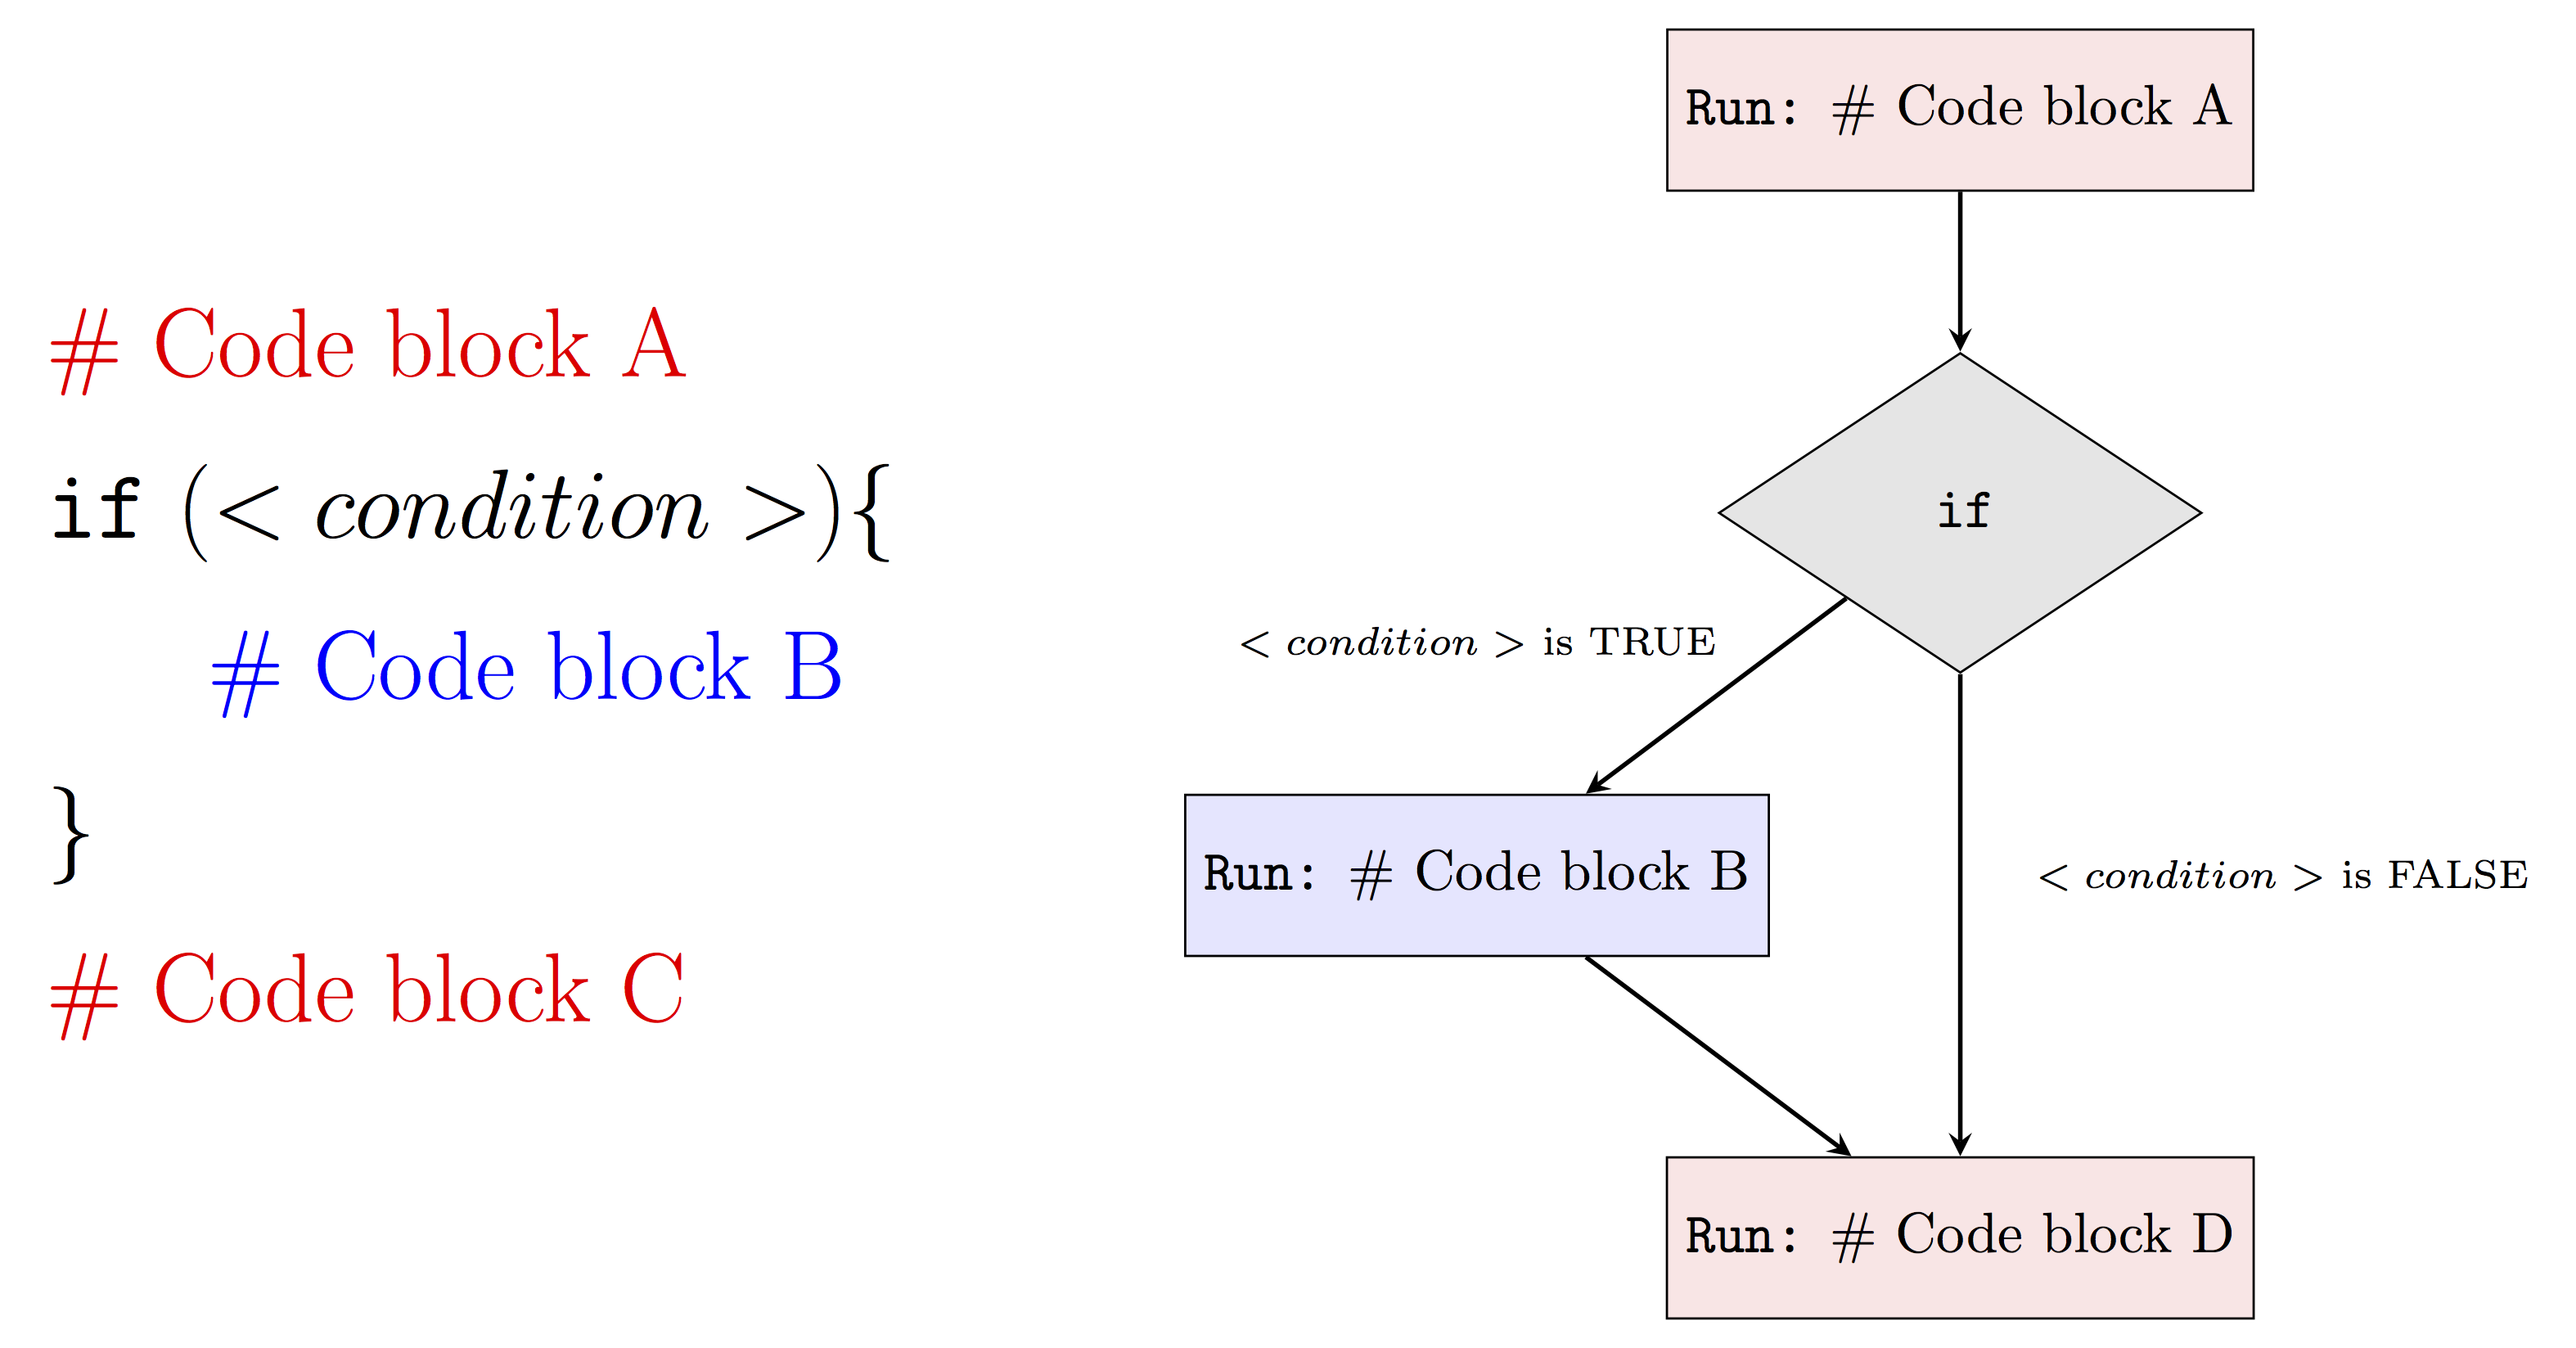
\includegraphics{images/if.png}

The \texttt{\textless{}conditon\textgreater{}} denotes a
\textbf{logical} variable that is used determine if the code inside of
\texttt{\{\ \}} will be evaluated. For example, if
\texttt{\textless{}condition\textgreater{}} is \texttt{FALSE} then our
program will run \texttt{Code\ block\ A} and then
\texttt{Code\ block\ C}. On the other hand, if
\texttt{\textless{}condition\textgreater{}} is \texttt{TRUE} our program
will run \texttt{Code\ block\ A}, \texttt{Code\ block\ B} and finally
\texttt{Code\ block\ C}.

Below we present two examples where two \texttt{if} statements are used.
In the first example, we use an \texttt{if} statement to compute the
absolute value of a variable called \texttt{x}:

\begin{Shaded}
\begin{Highlighting}[]
\NormalTok{x <-}\StringTok{ }\DecValTok{4}

\ControlFlowTok{if}\NormalTok{ (x }\OperatorTok{<}\StringTok{ }\DecValTok{0}\NormalTok{)\{}
\NormalTok{  x <-}\StringTok{ }\OperatorTok{-}\NormalTok{x}
\NormalTok{\}}

\NormalTok{x}
\end{Highlighting}
\end{Shaded}

\begin{verbatim}
## [1] 4
\end{verbatim}

Now we change \texttt{x} to a negative value:

\begin{Shaded}
\begin{Highlighting}[]
\NormalTok{x <-}\StringTok{ }\OperatorTok{-}\DecValTok{4}

\ControlFlowTok{if}\NormalTok{ (x }\OperatorTok{<}\StringTok{ }\DecValTok{0}\NormalTok{)\{}
\NormalTok{  x <-}\StringTok{ }\OperatorTok{-}\NormalTok{x}
\NormalTok{\}}

\NormalTok{x}
\end{Highlighting}
\end{Shaded}

\begin{verbatim}
## [1] 4
\end{verbatim}

In the second example, we use an \texttt{if} statement to assess if
\texttt{x} is an even number and, if this is the case, we print a simple
message.

\begin{Shaded}
\begin{Highlighting}[]
\ControlFlowTok{if}\NormalTok{ (x }\OperatorTok\StringTok{ }\DecValTok{2} \OperatorTok{==}\StringTok{ }\DecValTok{0}\NormalTok{)\{}
  \KeywordTok{print}\NormalTok{(}\KeywordTok{paste}\NormalTok{(x, }\StringTok{"is an even number"}\NormalTok{))}
\NormalTok{\}}
\end{Highlighting}
\end{Shaded}

\begin{verbatim}
## [1] "4 is an even number"
\end{verbatim}

\begin{Shaded}
\begin{Highlighting}[]
\NormalTok{x <-}\StringTok{ }\DecValTok{3}

\ControlFlowTok{if}\NormalTok{ (x }\OperatorTok\StringTok{ }\DecValTok{2} \OperatorTok{==}\StringTok{ }\DecValTok{0}\NormalTok{)\{}
  \KeywordTok{print}\NormalTok{(}\KeywordTok{paste}\NormalTok{(x, }\StringTok{"is an even number"}\NormalTok{))}
\NormalTok{\}}
\end{Highlighting}
\end{Shaded}

\subsubsection{\texorpdfstring{\texttt{if/else}
Statements}{if/else Statements}}\label{ifelse-statements}

Often when we write a program we want to tell R what to do when our
condition is \texttt{TRUE} and also what to do when it is
\texttt{FALSE}. Of course, we could do something like:

\begin{Shaded}
\begin{Highlighting}[]
\ControlFlowTok{if}\NormalTok{ (condition)\{}
\NormalTok{  plan A}
\NormalTok{\}}

\ControlFlowTok{if}\NormalTok{ (}\OperatorTok{!}\NormalTok{condition)\{}
\NormalTok{  plan B}
\NormalTok{\}}
\end{Highlighting}
\end{Shaded}

However, the above syntax is somewhat clumsy and one generally would
prefer to use an \texttt{if/else} statement. In plain English it would
correspond to something like, ``If this is true, then do plan A
otherwise do plan B''. In R we would write:

\begin{Shaded}
\begin{Highlighting}[]
\ControlFlowTok{if}\NormalTok{ (condition)\{}
\NormalTok{  plan A}
\NormalTok{\}}\ControlFlowTok{else}\NormalTok{\{}
\NormalTok{  plan B}
\NormalTok{\}}
\end{Highlighting}
\end{Shaded}

Similarly to an \texttt{if} statement, we can represent an
\texttt{if/else} statement using the diagram below:

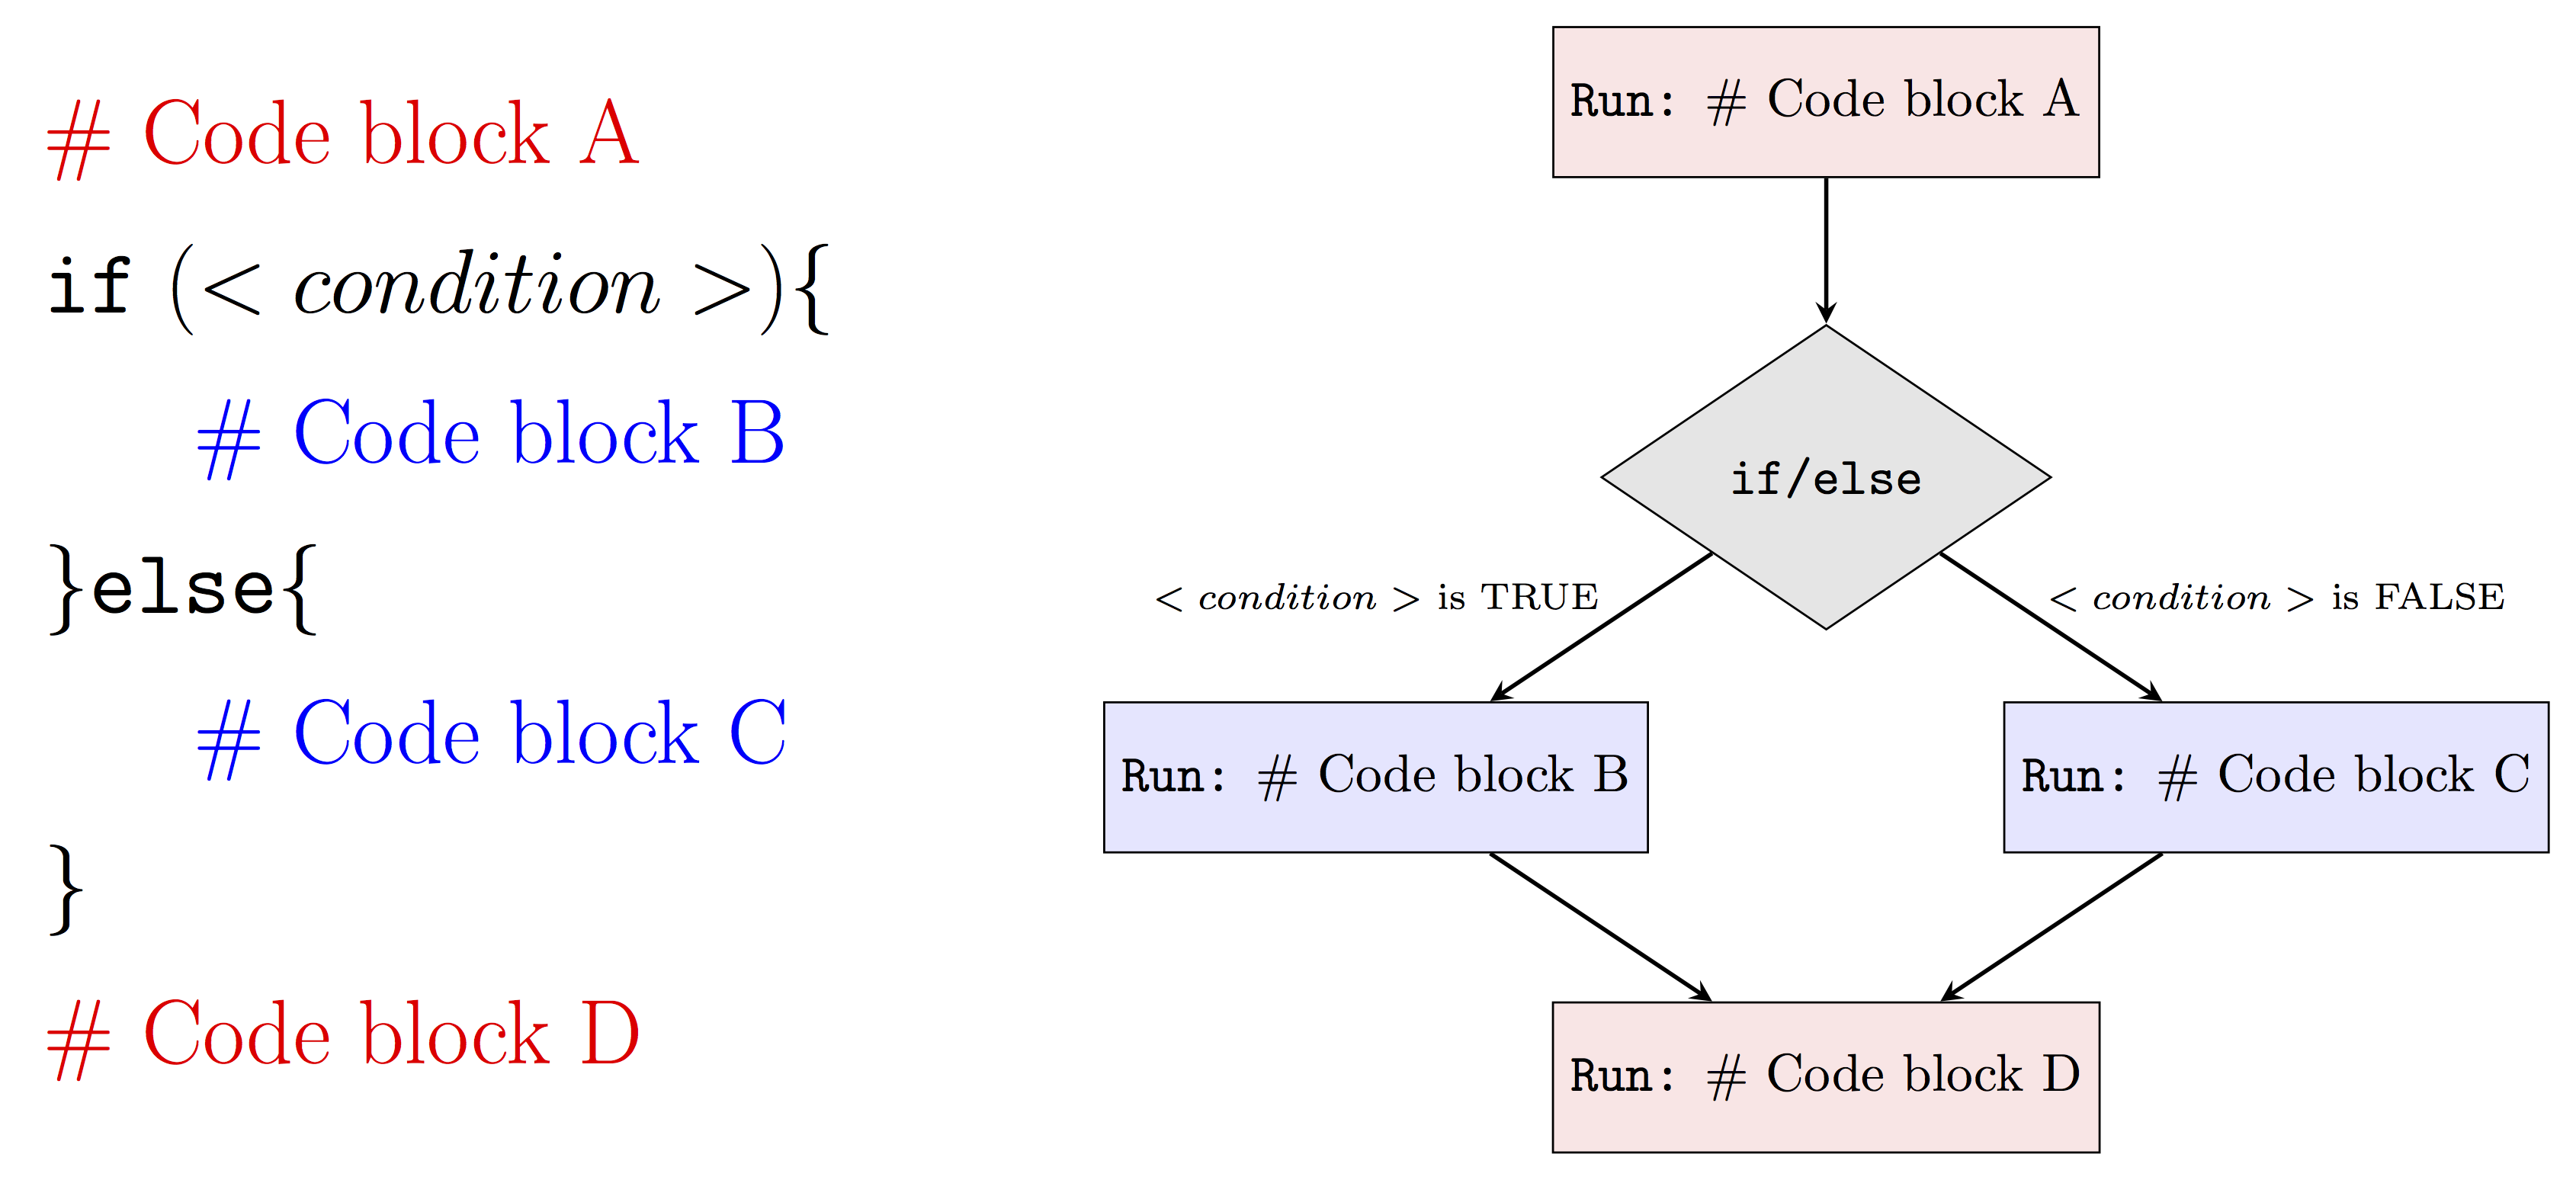
\includegraphics{images/ifelse.png}

Therefore, when \texttt{\textless{}condition\textgreater{}} is
\texttt{TRUE} our program will run \texttt{Code\ block\ A},
\texttt{Code\ block\ B} and then \texttt{Code\ block\ D} while when
\texttt{\textless{}condition\textgreater{}} is \texttt{FALSE} it will
run \texttt{Code\ block\ A}, \texttt{Code\ block\ B} and finally
\texttt{Code\ block\ D}. Using this new tool we can revisit our previous
example on even numbers to include a custom message in the case of an
odd number. This can be done as follows:

\begin{Shaded}
\begin{Highlighting}[]
\NormalTok{x <-}\StringTok{ }\DecValTok{2}

\ControlFlowTok{if}\NormalTok{ (x }\OperatorTok\StringTok{ }\DecValTok{2} \OperatorTok{==}\StringTok{ }\DecValTok{0}\NormalTok{)\{}
  \KeywordTok{print}\NormalTok{(}\KeywordTok{paste}\NormalTok{(x, }\StringTok{"is an even number"}\NormalTok{))}
\NormalTok{\}}\ControlFlowTok{else}\NormalTok{\{}
  \KeywordTok{print}\NormalTok{(}\KeywordTok{paste}\NormalTok{(x, }\StringTok{"is an odd number"}\NormalTok{))}
\NormalTok{\}}
\end{Highlighting}
\end{Shaded}

\begin{verbatim}
## [1] "2 is an even number"
\end{verbatim}

\begin{Shaded}
\begin{Highlighting}[]
\NormalTok{x <-}\StringTok{ }\DecValTok{3}

\ControlFlowTok{if}\NormalTok{ (x }\OperatorTok\StringTok{ }\DecValTok{2} \OperatorTok{==}\StringTok{ }\DecValTok{0}\NormalTok{)\{}
  \KeywordTok{print}\NormalTok{(}\KeywordTok{paste}\NormalTok{(x, }\StringTok{"is an even number"}\NormalTok{))}
\NormalTok{\}}\ControlFlowTok{else}\NormalTok{\{}
  \KeywordTok{print}\NormalTok{(}\KeywordTok{paste}\NormalTok{(x, }\StringTok{"is an odd number"}\NormalTok{))}
\NormalTok{\}}
\end{Highlighting}
\end{Shaded}

\begin{verbatim}
## [1] "3 is an odd number"
\end{verbatim}

\subsubsection{\texorpdfstring{\texttt{if/elseif/else}
Statements}{if/elseif/else Statements}}\label{ifelseifelse-statements}

We can also control the flow of statements with multiple if/else
statements, depending on the number of cases we consider. Typically, the
more cases we have, the more else if statements. An example
visualization is provided below.

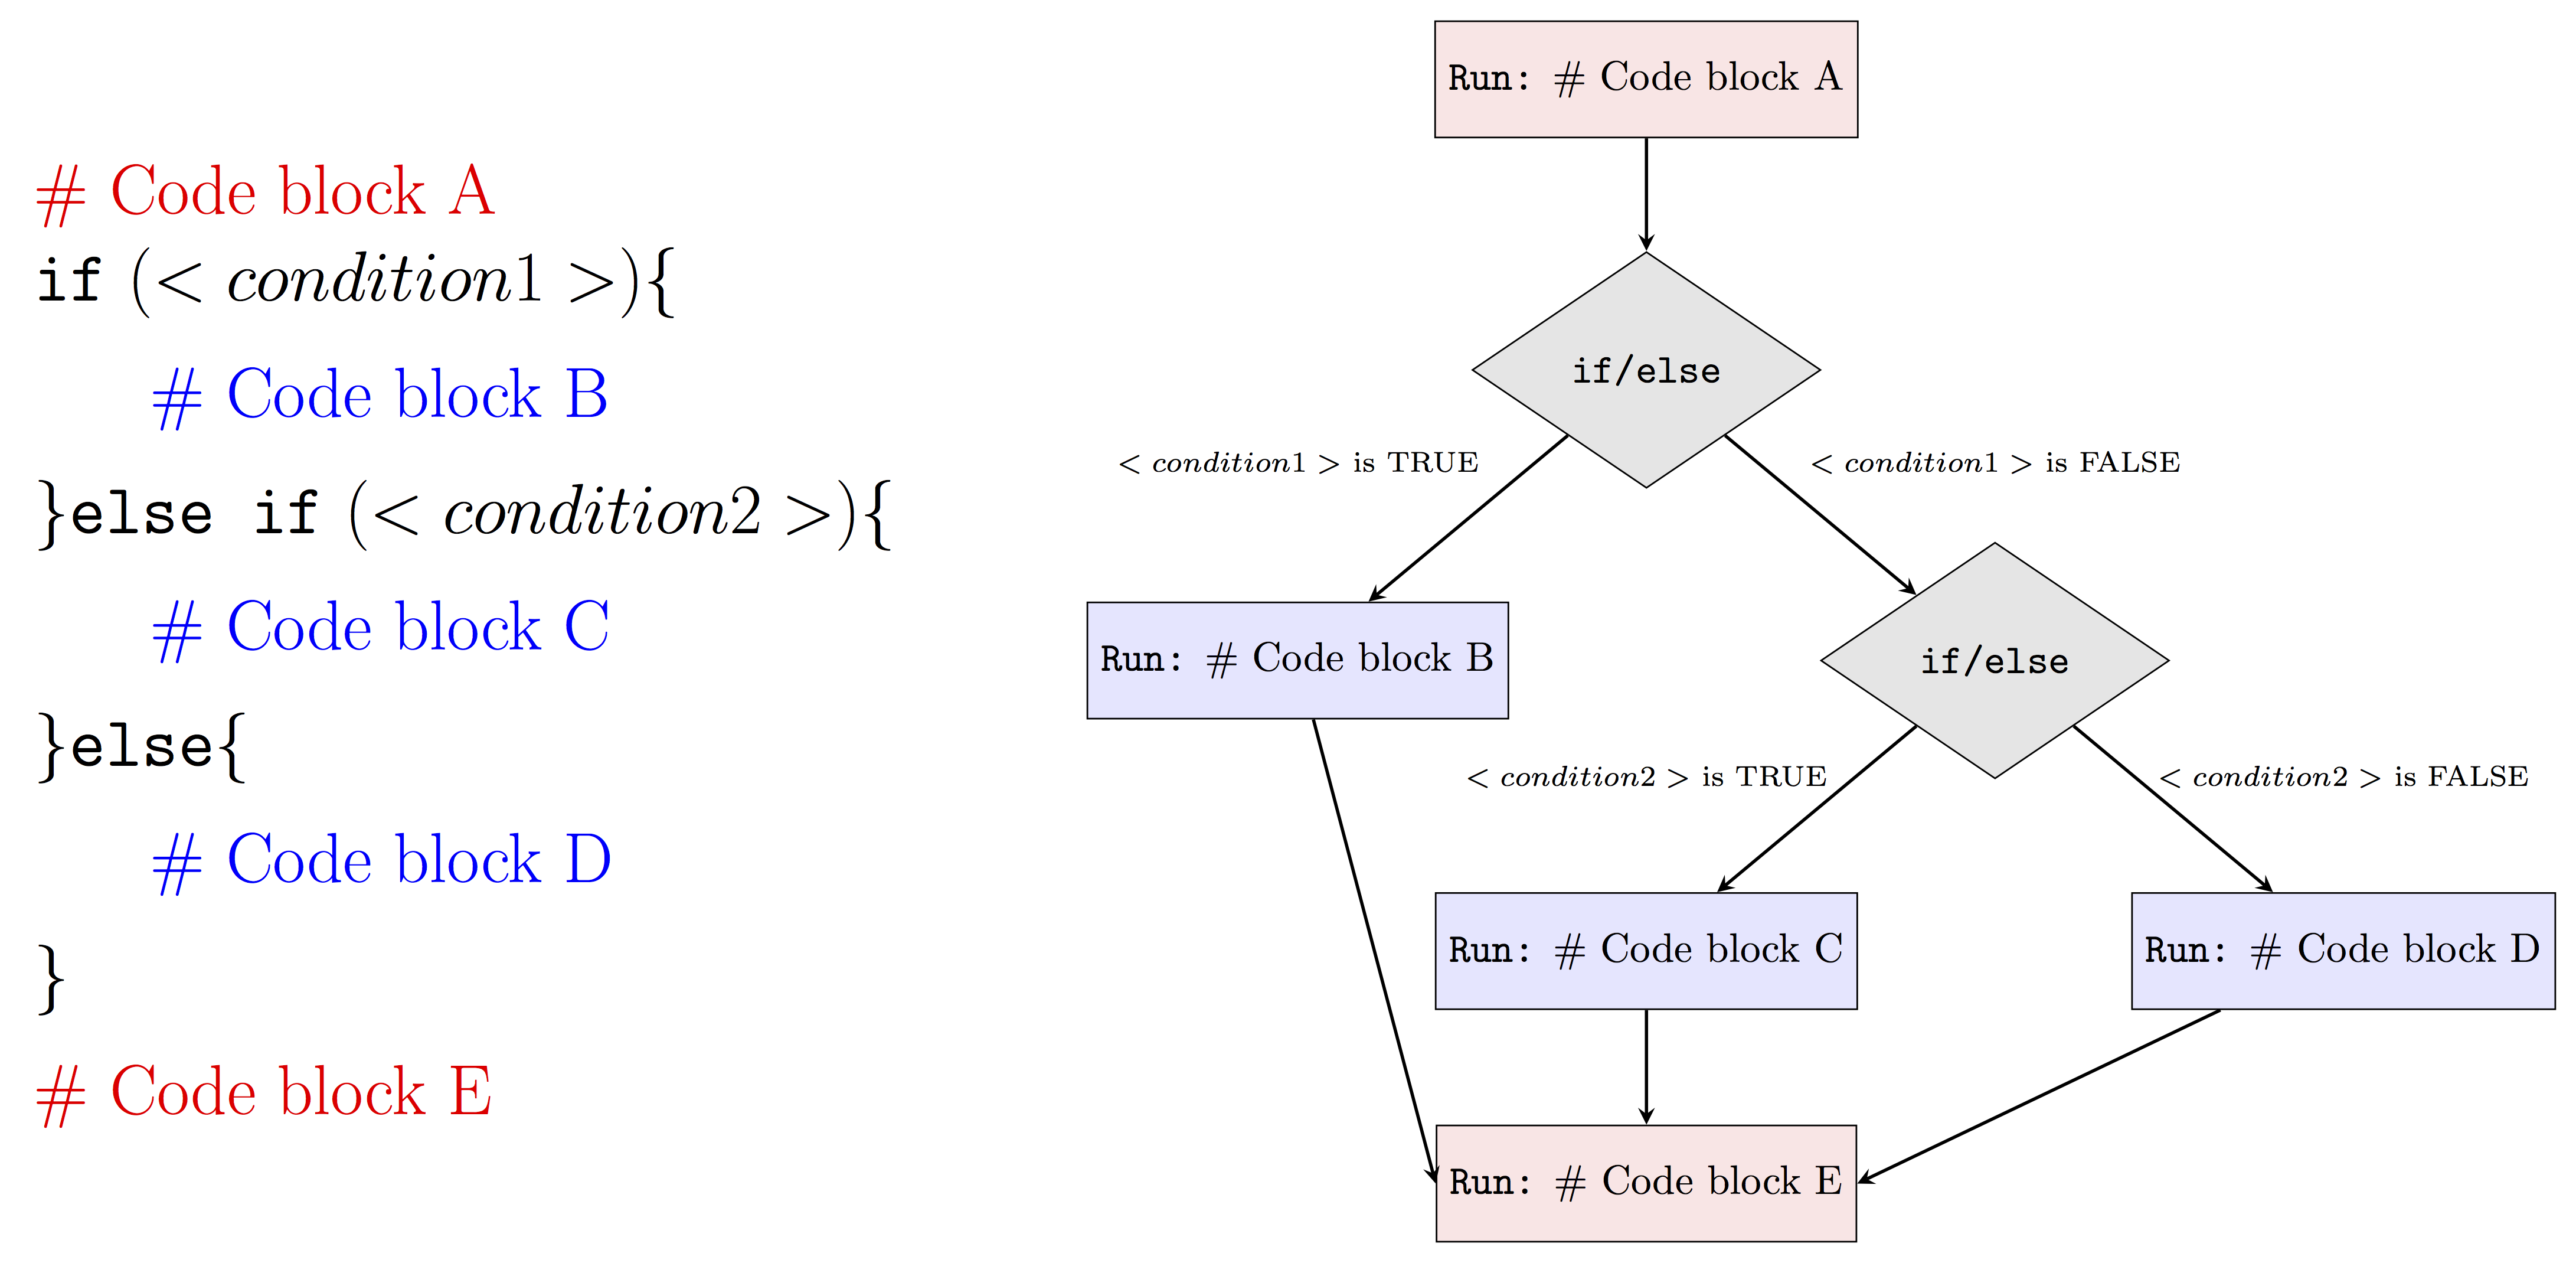
\includegraphics{images/ifelseifelse.png}

\subsubsection{\texorpdfstring{\texttt{switch}
Statement}{switch Statement}}\label{switch-statement}

Earlier we mentioned that if/elseif/else statements allow us to choose
between TRUE and FALSE when there are two options. With the above idea,
when there are more than two options we can simply use nested if/else
statements. What about when we have roughly 20 options to choose from?
In this case, if we stick to using nested if/else statements, the
programming logic will be very difficult to understand. The switch
statement option in R programming can help us handle this type of
problems more effectively.

Before we put switch statements into the case study, let's first start
to understand the basic switch statement syntax in R.

\begin{Shaded}
\begin{Highlighting}[]
\ControlFlowTok{switch}\NormalTok{ (Expression,}
        \StringTok{"Option 1"}\NormalTok{ =}\StringTok{ }\NormalTok{Execute this statement when the expression result matches Option }\DecValTok{1}\NormalTok{,}
        \StringTok{"Option 2"}\NormalTok{ =}\StringTok{ }\NormalTok{Execute this statement when the expression result matches Option }\DecValTok{2}\NormalTok{,}
        \StringTok{"Option 3"}\NormalTok{ =}\StringTok{ }\NormalTok{Execute this statement when the expression result matches Option }\DecValTok{3}\NormalTok{,}
\NormalTok{        ....}
\NormalTok{        ....}
        \StringTok{"Option N"}\NormalTok{ =}\StringTok{ }\NormalTok{Execute this statement when the expression result matches Option N,}
\NormalTok{        Default Statements}
\NormalTok{)}
\end{Highlighting}
\end{Shaded}

\begin{itemize}
\tightlist
\item
  The \texttt{expression} value is the condition which R will evaluate.
  This should be either integer or character.
\item
  When the \texttt{expression} value matches more than one option, the
  first matching statement will be returned.
\item
  Besides the conditional statement, R also allows us to add the
  \texttt{default\ statement}, which will be returned when none of the
  listed options are matched.
\end{itemize}

With the above syntax in mind, let's now check a simple case study with
R switch statements.

\begin{Shaded}
\begin{Highlighting}[]
\NormalTok{number1 <-}\StringTok{ }\DecValTok{20}
\NormalTok{number2 <-}\StringTok{ }\DecValTok{5}
\NormalTok{operator =}\StringTok{ }\KeywordTok{readline}\NormalTok{(}\DataTypeTok{prompt=}\StringTok{"Please enter any ARITHMETIC OPERATOR: "}\NormalTok{)}

\ControlFlowTok{switch}\NormalTok{(operator,}
       \StringTok{"+"}\NormalTok{ =}\StringTok{ }\KeywordTok{print}\NormalTok{(}\KeywordTok{paste}\NormalTok{(}\StringTok{"Addition of two numbers is: "}\NormalTok{, number1 }\OperatorTok{+}\StringTok{ }\NormalTok{number2)),}
       \StringTok{"-"}\NormalTok{ =}\StringTok{ }\KeywordTok{print}\NormalTok{(}\KeywordTok{paste}\NormalTok{(}\StringTok{"Subtraction of two numbers is: "}\NormalTok{, number1 }\OperatorTok{-}\StringTok{ }\NormalTok{number2)),}
       \StringTok{"*"}\NormalTok{ =}\StringTok{ }\KeywordTok{print}\NormalTok{(}\KeywordTok{paste}\NormalTok{(}\StringTok{"Multiplication of two numbers is: "}\NormalTok{, number1 }\OperatorTok{*}\StringTok{ }\NormalTok{number2)),}
       \StringTok{"/"}\NormalTok{ =}\StringTok{ }\KeywordTok{print}\NormalTok{(}\KeywordTok{paste}\NormalTok{(}\StringTok{"Division of two numbers is: "}\NormalTok{, number1 }\OperatorTok{/}\StringTok{ }\NormalTok{number2))}
\NormalTok{)}
\end{Highlighting}
\end{Shaded}

When running the above code in R, we can expect results like:

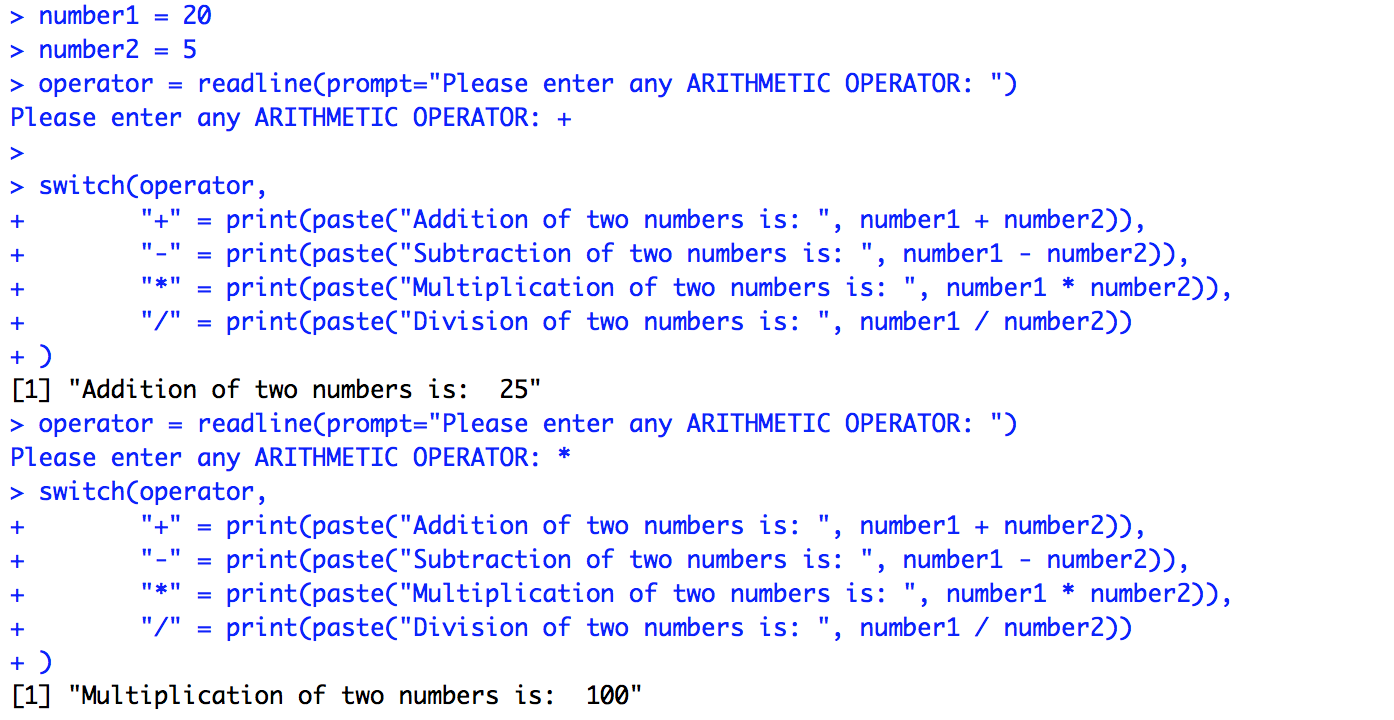
\includegraphics{images/switch_example.png}

In conclusion, we can visualize the R switch statement as follows:

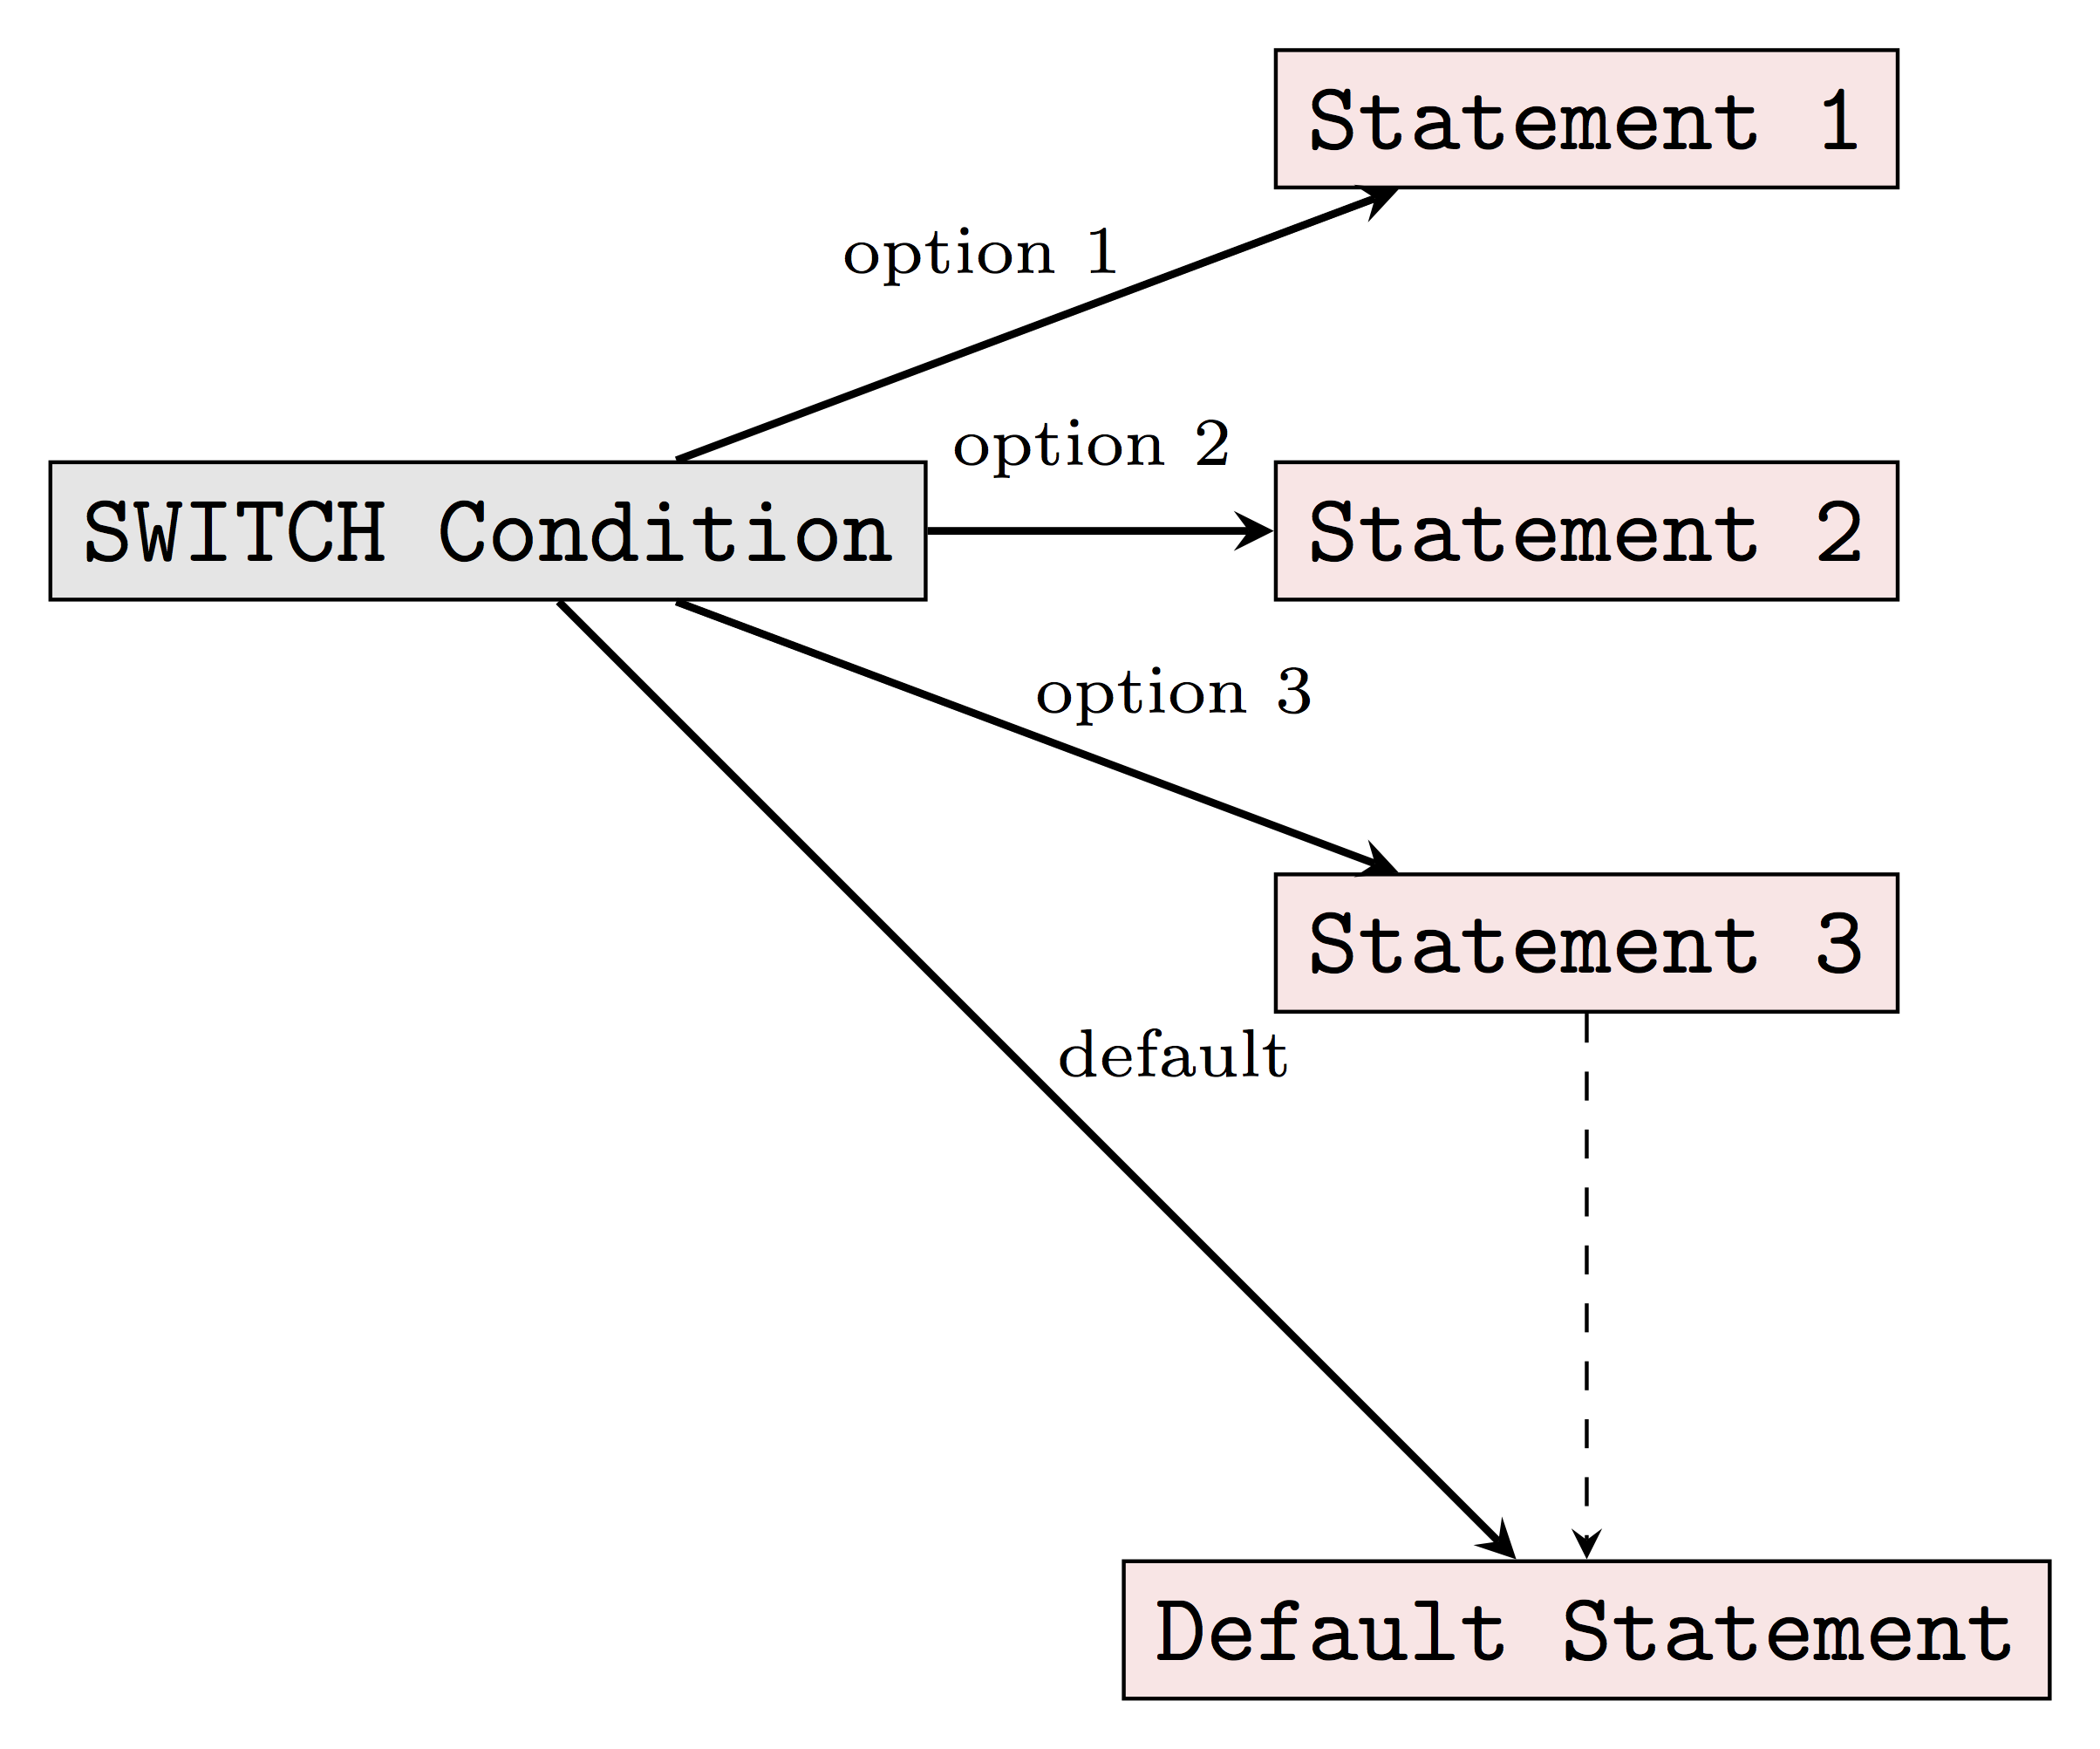
\includegraphics{images/flowchart_switch.png}

\subsection{Iterative Control Statements}\label{iter_cont_stat}

Iterative control statements are an extremly useful R method for
repeating a task multiple times. For example, pretend we are trying to
build a program that solves a simple maze like the one below.

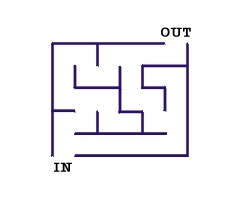
\includegraphics{images/maze.jpg}

It would be pretty easy to simply draw out the possible solutions with
the naked eye. However, if you were actually inside the maze, you would
need to narrow your perspective and think of a strategy, like marking
paths you have already visited. Suppose that we have a strategy in mind
to solve this problem. For example, we could consider the following
approach at any given point in time:

\begin{itemize}
\tightlist
\item
  if there is space in front of you, go forward
\item
  else, if there is space on your right, turn right
\item
  else, if there is space on your left, turn left
\item
  else, {[}all three sides (forward, left, right) are closed{]} turn
  around
\end{itemize}

This strategy could easily be programmed using the methods discussed in
Section \ref{selcontrostat} but to actually program it you would need to
repeat this strategy until you escaped the maze. Your strategy could for
example be written as:

\begin{Shaded}
\begin{Highlighting}[]
\ControlFlowTok{repeat}\NormalTok{ (until }\StringTok{"you are free"}\NormalTok{)\{}
  \ControlFlowTok{if}\NormalTok{ (}\StringTok{"space in front of you"}\NormalTok{)\{}
\NormalTok{    go forward}
\NormalTok{  \}}\ControlFlowTok{else} \ControlFlowTok{if}\NormalTok{ (}\StringTok{"space on your right"}\NormalTok{)\{}
\NormalTok{    turn right }
\NormalTok{  \}}\ControlFlowTok{else} \ControlFlowTok{if}\NormalTok{ (}\StringTok{"space on your left"}\NormalTok{)\{}
\NormalTok{    turn left}
\NormalTok{  \}}\ControlFlowTok{else}\NormalTok{\{}
\NormalTok{    turn around}
\NormalTok{  \}}
\NormalTok{\}}
\end{Highlighting}
\end{Shaded}

Try to develop an algorithm to exit the maze presented above. Could you
escape? Though it might take some time (and probably would not
correspond to the fastest strategy) one can show that this method can
solve any maze (assuming of course that a solution exists). In this
section we discuss the elements necessary to actually program the
``\texttt{repeat\ (until\ "you\ are\ free")}'' part of our algorithm.

\subsubsection{\texorpdfstring{\texttt{for}
Loops}{for Loops}}\label{forloop}

Let's consider the following situation:

\begin{Shaded}
\begin{Highlighting}[]
\KeywordTok{print}\NormalTok{(}\DecValTok{1}\NormalTok{)}
\KeywordTok{print}\NormalTok{(}\DecValTok{2}\NormalTok{)}
\KeywordTok{print}\NormalTok{(}\DecValTok{3}\NormalTok{)}
\KeywordTok{print}\NormalTok{(}\DecValTok{4}\NormalTok{)}
\KeywordTok{print}\NormalTok{(}\DecValTok{5}\NormalTok{)}
\KeywordTok{print}\NormalTok{(}\DecValTok{6}\NormalTok{)}
\end{Highlighting}
\end{Shaded}

This seems feasible when we only need to print out the numbers from 1 to
6. What if we want to print out the numbers from 1 to 100? It is such a
clumsy and tedious approach if we keep repeating \texttt{print()} line
by line to do so.

For loops in R help us solve this type of problems much more effectively
in only a couple lines of codes. It allows us to repeat the same part of
code, or say a sequence of same instructions, under certain conditions
without explicitly writing out the code everytime. For example, to do
exactly the same as the above example with for loops, all we need is:

\begin{Shaded}
\begin{Highlighting}[]
\ControlFlowTok{for}\NormalTok{ (number }\ControlFlowTok{in} \DecValTok{1}\OperatorTok{:}\DecValTok{6}\NormalTok{)\{}
  \KeywordTok{print}\NormalTok{(number)}
\NormalTok{\}}
\end{Highlighting}
\end{Shaded}

\begin{verbatim}
## [1] 1
## [1] 2
## [1] 3
## [1] 4
## [1] 5
## [1] 6
\end{verbatim}

To interpret the above for loops in plain English, we can read it as
``When the number is in the sequence \{1,2,3,4,5,6\}, we will print this
number until we exhaust all numbers in the sequence''. As we can see
obviously, this approach simplifies our code so much more as we only
need to write the code chunk (\texttt{print()} in this case) once, not
six times, not to mention when we want to print out all the numbers from
1 to 100 compared to repeating \texttt{print()} line by line for 100
times.

The basic syntax of for loops in R is as follows:

\begin{Shaded}
\begin{Highlighting}[]
\ControlFlowTok{for}\NormalTok{ (some specified sequence to loop over)\{}
\NormalTok{  execute this statement when we still haven not reached the last item }\ControlFlowTok{in}\NormalTok{ the sequence}
\NormalTok{\}}
\end{Highlighting}
\end{Shaded}

\texttt{Next} also helps when you want to skip for some cases in which
you don't want the statement to be executed. To see how \texttt{next}
works together with for loops in R, let's consider the following more
mathematical example when you want to print out all the odd numbers
between 1 to 10.

\begin{Shaded}
\begin{Highlighting}[]
\ControlFlowTok{for}\NormalTok{ (i }\ControlFlowTok{in} \DecValTok{1}\OperatorTok{:}\DecValTok{10}\NormalTok{) \{}
  \ControlFlowTok{if}\NormalTok{ (}\OperatorTok{!}\NormalTok{i }\OperatorTok\StringTok{ }\DecValTok{2}\NormalTok{)\{}
    \ControlFlowTok{next}
\NormalTok{  \}}
  \KeywordTok{print}\NormalTok{(i)}
\NormalTok{\}}
\end{Highlighting}
\end{Shaded}

\begin{verbatim}
## [1] 1
## [1] 3
## [1] 5
## [1] 7
## [1] 9
\end{verbatim}

From the results, we notice that R automatically skip to run
\texttt{print(i)} when \texttt{!i\ \%\%2} is TRUE. To interpret the
above in plain English, we can read it as ``if the number i cannot be
divided by 2, we skip the below and consider the NEXT number in the
sequence''. In this case, we can still use for loops when we have some
exceptional cases.

In conclusion, we can visualize the R for loops as follows:

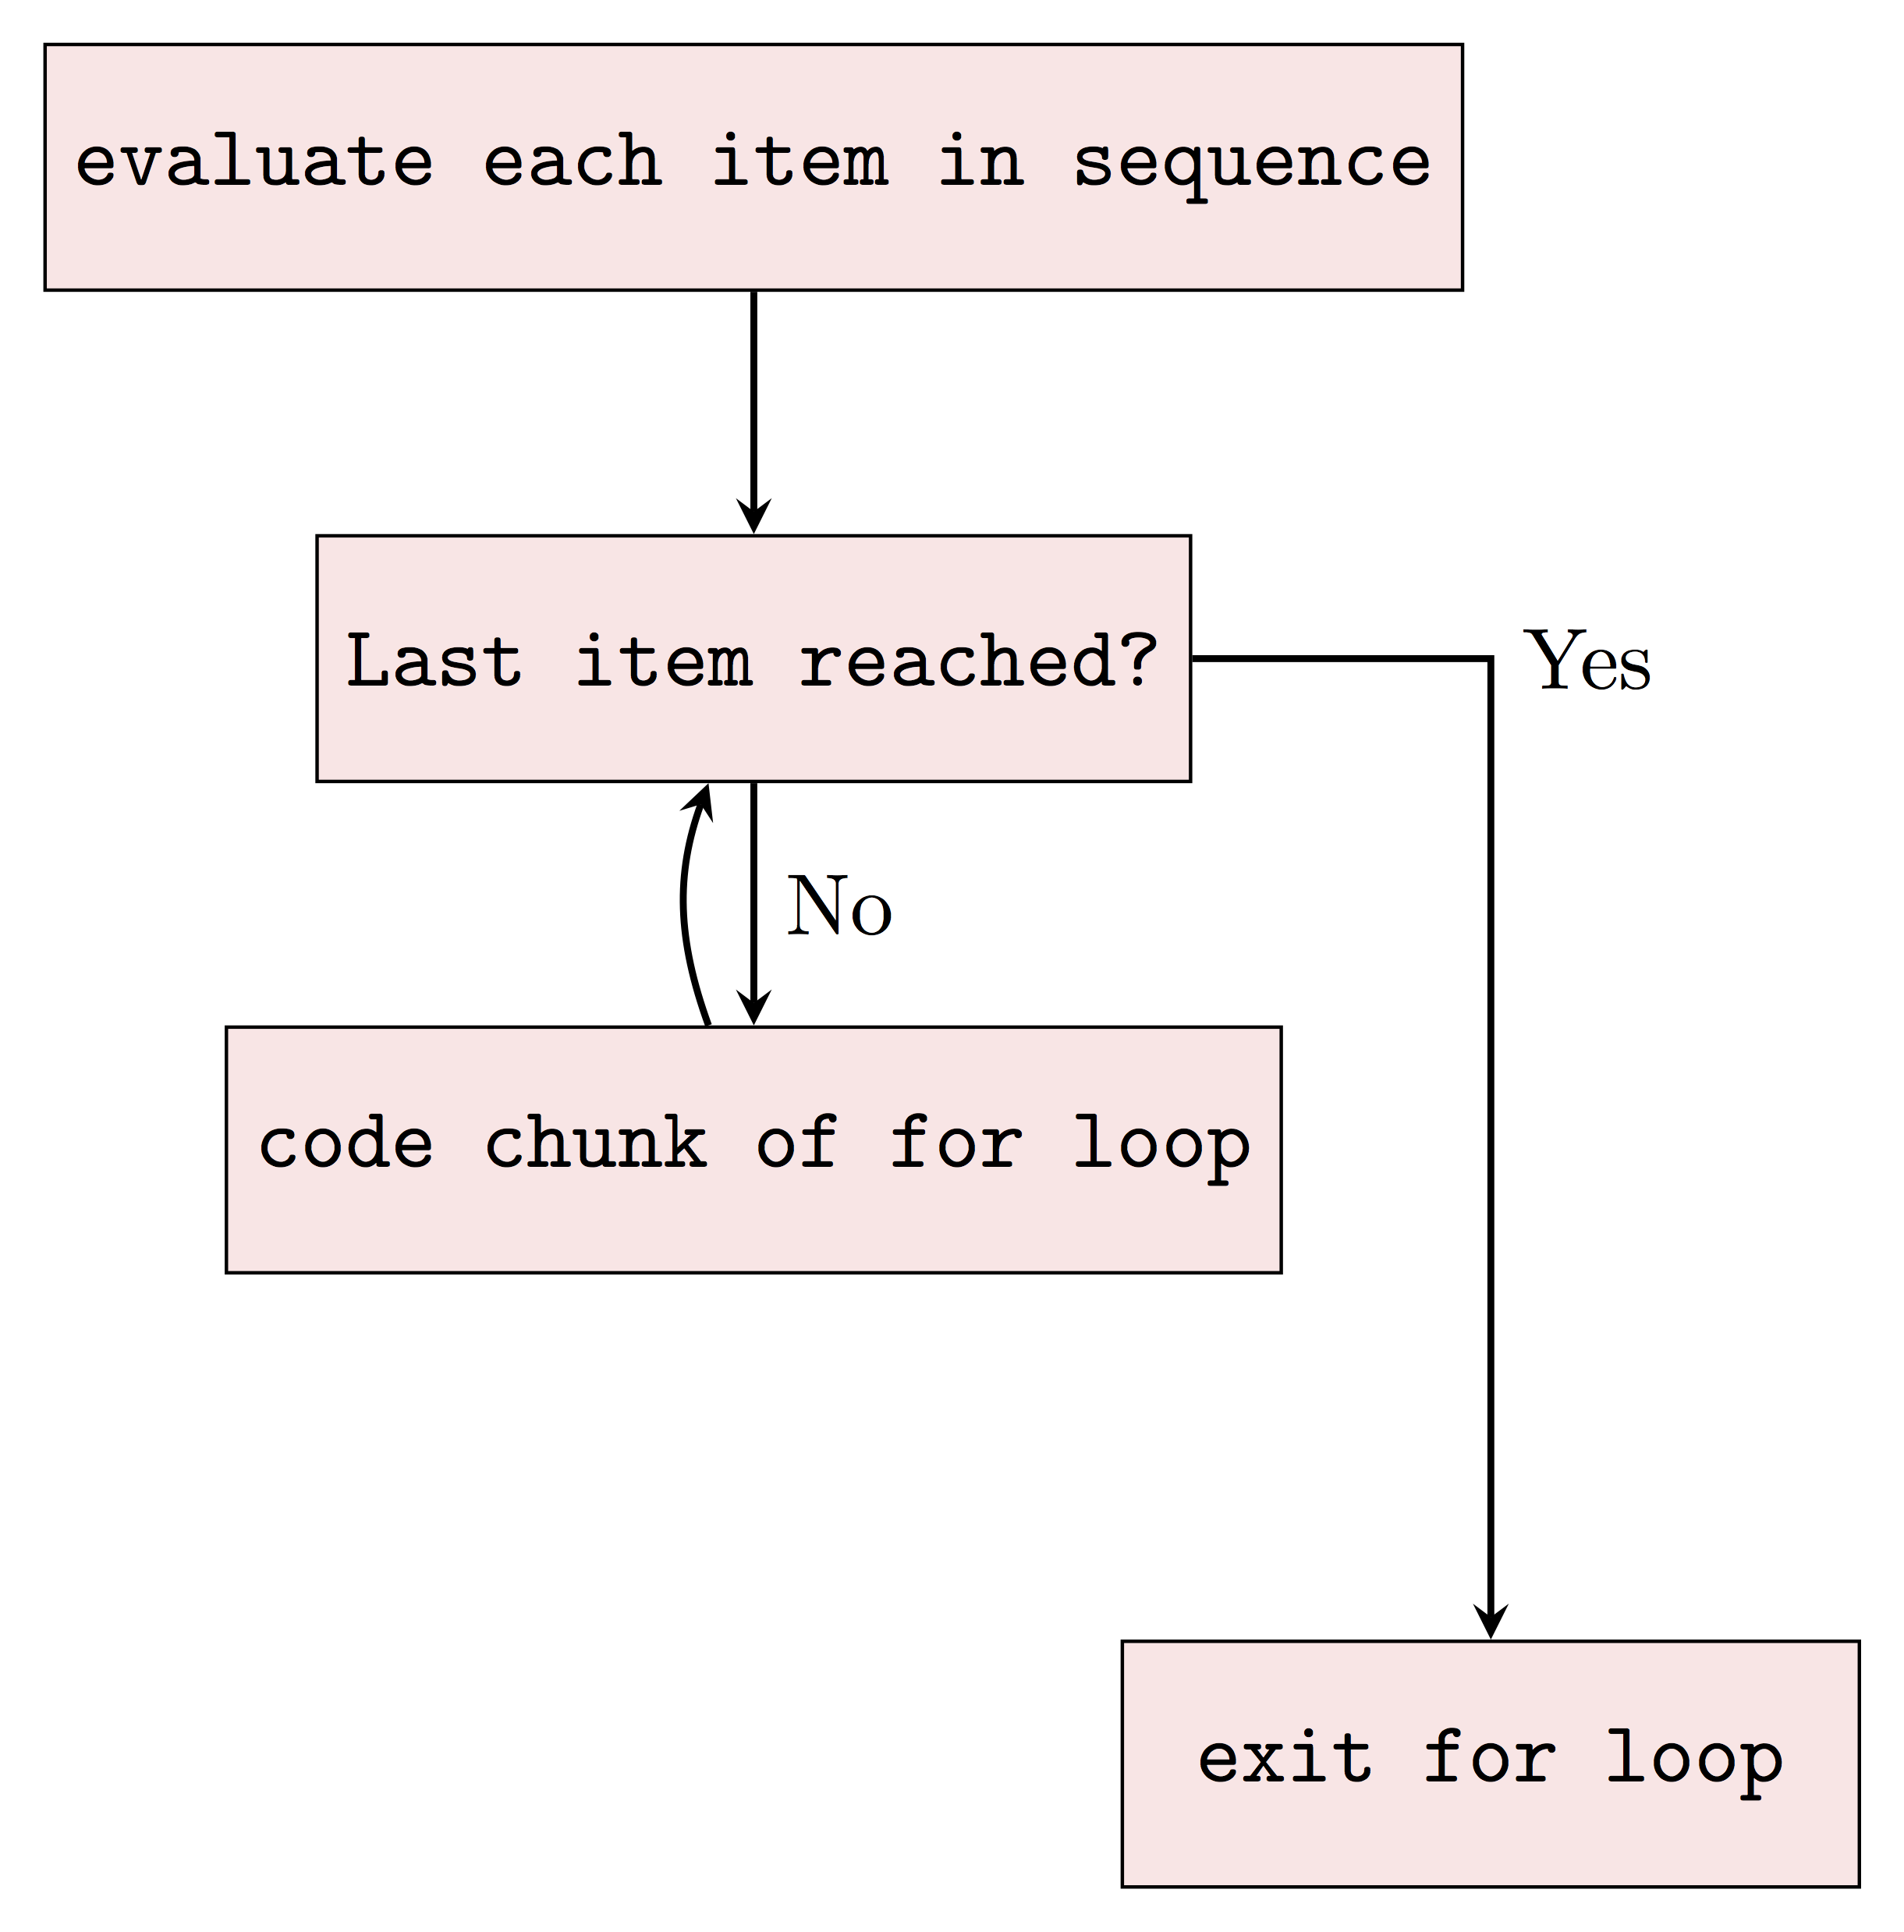
\includegraphics{images/flowchart___for_loop.png}

Up till now, we can see that for loops can simplify our work a lot when
we need to execute a sequence of same instructions for multiple times.
However, there are still disadvantages to use for loops in R. We may
hardly notice now with only a few simple iterations to run. But indeed,
R can be very slow when running iteration, especially when we need to do
a lot of big iterations with big data. Sometimes we may prefer to avoid
using for loops in R by using other approaches since R supports
vectorization, which will allow for much faster calculations. For
example, solutions that make use of loops are less efficient than
vectorized solutions that make use of apply functions, such as lapply
and sapply. It's often better to use the latter.

Apply methods are often used to make operations on some structured data.
For example, let's simulate a matrix of some random samples.

\begin{Shaded}
\begin{Highlighting}[]
\NormalTok{(}\DataTypeTok{exp_mat =} \KeywordTok{matrix}\NormalTok{(}\KeywordTok{rnorm}\NormalTok{(}\DecValTok{60}\NormalTok{),}\DataTypeTok{ncol =} \DecValTok{3}\NormalTok{))}
\end{Highlighting}
\end{Shaded}

\begin{verbatim}
##              [,1]        [,2]        [,3]
##  [1,]  0.94264912  0.97129400  1.68529946
##  [2,] -1.54433424 -0.12059055  1.22173473
##  [3,]  1.92951252 -1.04643002  0.61444018
##  [4,] -0.75991686  0.20699467  0.86218858
##  [5,]  1.08951791 -0.06078078 -1.06752316
##  [6,] -0.35065936 -0.57768288  1.03731534
##  [7,] -0.18588595 -0.40293968  0.38930071
##  [8,]  0.26631478 -2.22241120  0.19439612
##  [9,]  0.07945905 -1.08220515 -0.47541793
## [10,]  0.62391283  1.88244921  0.26669057
## [11,] -1.37242333  0.22497235 -0.52147618
## [12,] -0.22614800  0.08530340  0.20213233
## [13,] -0.15417994 -0.70940862  0.37684181
## [14,] -0.28688260  1.12938605 -1.35845137
## [15,] -1.14549570  0.46605330  1.11646689
## [16,] -0.57833306  0.29616826 -1.24839644
## [17,]  1.20423147  0.69292618 -1.84019251
## [18,]  0.77388894 -0.11523996  1.53426210
## [19,]  1.79602743 -0.18210614 -1.66679156
## [20,] -0.54578433  0.08785389 -0.04871862
\end{verbatim}

To get the mean of each column, we can calculate each column mean
separately or use a for loop.

\begin{Shaded}
\begin{Highlighting}[]
\CommentTok{# Observe what this does}
\KeywordTok{mean}\NormalTok{(exp_mat)}
\end{Highlighting}
\end{Shaded}

\begin{verbatim}
## [1] 0.03921963
\end{verbatim}

\begin{Shaded}
\begin{Highlighting}[]
\CommentTok{# Calculate separately }
\KeywordTok{mean}\NormalTok{(exp_mat[,}\DecValTok{1}\NormalTok{])}
\end{Highlighting}
\end{Shaded}

\begin{verbatim}
## [1] 0.07777353
\end{verbatim}

\begin{Shaded}
\begin{Highlighting}[]
\KeywordTok{mean}\NormalTok{(exp_mat[,}\DecValTok{2}\NormalTok{])}
\end{Highlighting}
\end{Shaded}

\begin{verbatim}
## [1] -0.02381968
\end{verbatim}

\begin{Shaded}
\begin{Highlighting}[]
\KeywordTok{mean}\NormalTok{(exp_mat[,}\DecValTok{3}\NormalTok{])}
\end{Highlighting}
\end{Shaded}

\begin{verbatim}
## [1] 0.06370505
\end{verbatim}

\begin{Shaded}
\begin{Highlighting}[]
\CommentTok{# Using a for loop }
\ControlFlowTok{for}\NormalTok{(i }\ControlFlowTok{in} \DecValTok{1}\OperatorTok{:}\DecValTok{3}\NormalTok{)\{}
  \KeywordTok{print}\NormalTok{(}\KeywordTok{mean}\NormalTok{(exp_mat[,i]))}
\NormalTok{\}}
\end{Highlighting}
\end{Shaded}

\begin{verbatim}
## [1] 0.07777353
## [1] -0.02381968
## [1] 0.06370505
\end{verbatim}

However, using \texttt{apply}, we can do this in a very simple manner.

\begin{Shaded}
\begin{Highlighting}[]
\KeywordTok{apply}\NormalTok{(exp_mat, }\DecValTok{2}\NormalTok{, mean) }
\end{Highlighting}
\end{Shaded}

\begin{verbatim}
## [1]  0.07777353 -0.02381968  0.06370505
\end{verbatim}

\begin{Shaded}
\begin{Highlighting}[]
\CommentTok{# The 2 indicates operations on columns and not rows }
\end{Highlighting}
\end{Shaded}

We will see how these approaches can help accelerate our work later.

\subsubsection{\texorpdfstring{\texttt{while}
Statements}{while Statements}}\label{while-statements}

As an alternative of for loops, while statement in R is another approach
that can help us repeat the code chunk only when specific conditions are
satisfied. For example, we can use while statement to do exactly the
same as above to print out all numbers from 1 to 6 as followings:

\begin{Shaded}
\begin{Highlighting}[]
\NormalTok{i =}\StringTok{ }\DecValTok{1}
\ControlFlowTok{while}\NormalTok{ (i }\OperatorTok{<=}\StringTok{ }\DecValTok{6}\NormalTok{)\{}
  \KeywordTok{print}\NormalTok{(i)}
\NormalTok{  i =}\StringTok{ }\NormalTok{i}\OperatorTok{+}\DecValTok{1}
\NormalTok{\}}
\end{Highlighting}
\end{Shaded}

\begin{verbatim}
## [1] 1
## [1] 2
## [1] 3
## [1] 4
## [1] 5
## [1] 6
\end{verbatim}

The above code can be interprented in plain English as: ``Let's start
with number 1. When the number i is still smaller than or equal to 6, we
print it out. Then we consider the next integer of it and stop when we
finish all the numbers smaller than or equal to 6.''

As we can see, while statement is used to iterate until a specific
condition is met. To make use of while statement in R, we introduce the
basic syntax of it as following:

\begin{Shaded}
\begin{Highlighting}[]
\ControlFlowTok{while}\NormalTok{ (some specified condition)}
\NormalTok{\{}
\NormalTok{   statement to execute when the above condition is satisfied}
\NormalTok{\}}
\end{Highlighting}
\end{Shaded}

Here we evaluate the condition and if it is \texttt{TRUE}, then we
execute the statement inside the code chunk. Once we finish running the
statement, we evaluate the condition again and exit the loops when the
condition is evaluated as \texttt{FALSE}.

In conclusion, we can visualize how the while statement works in R as
following:

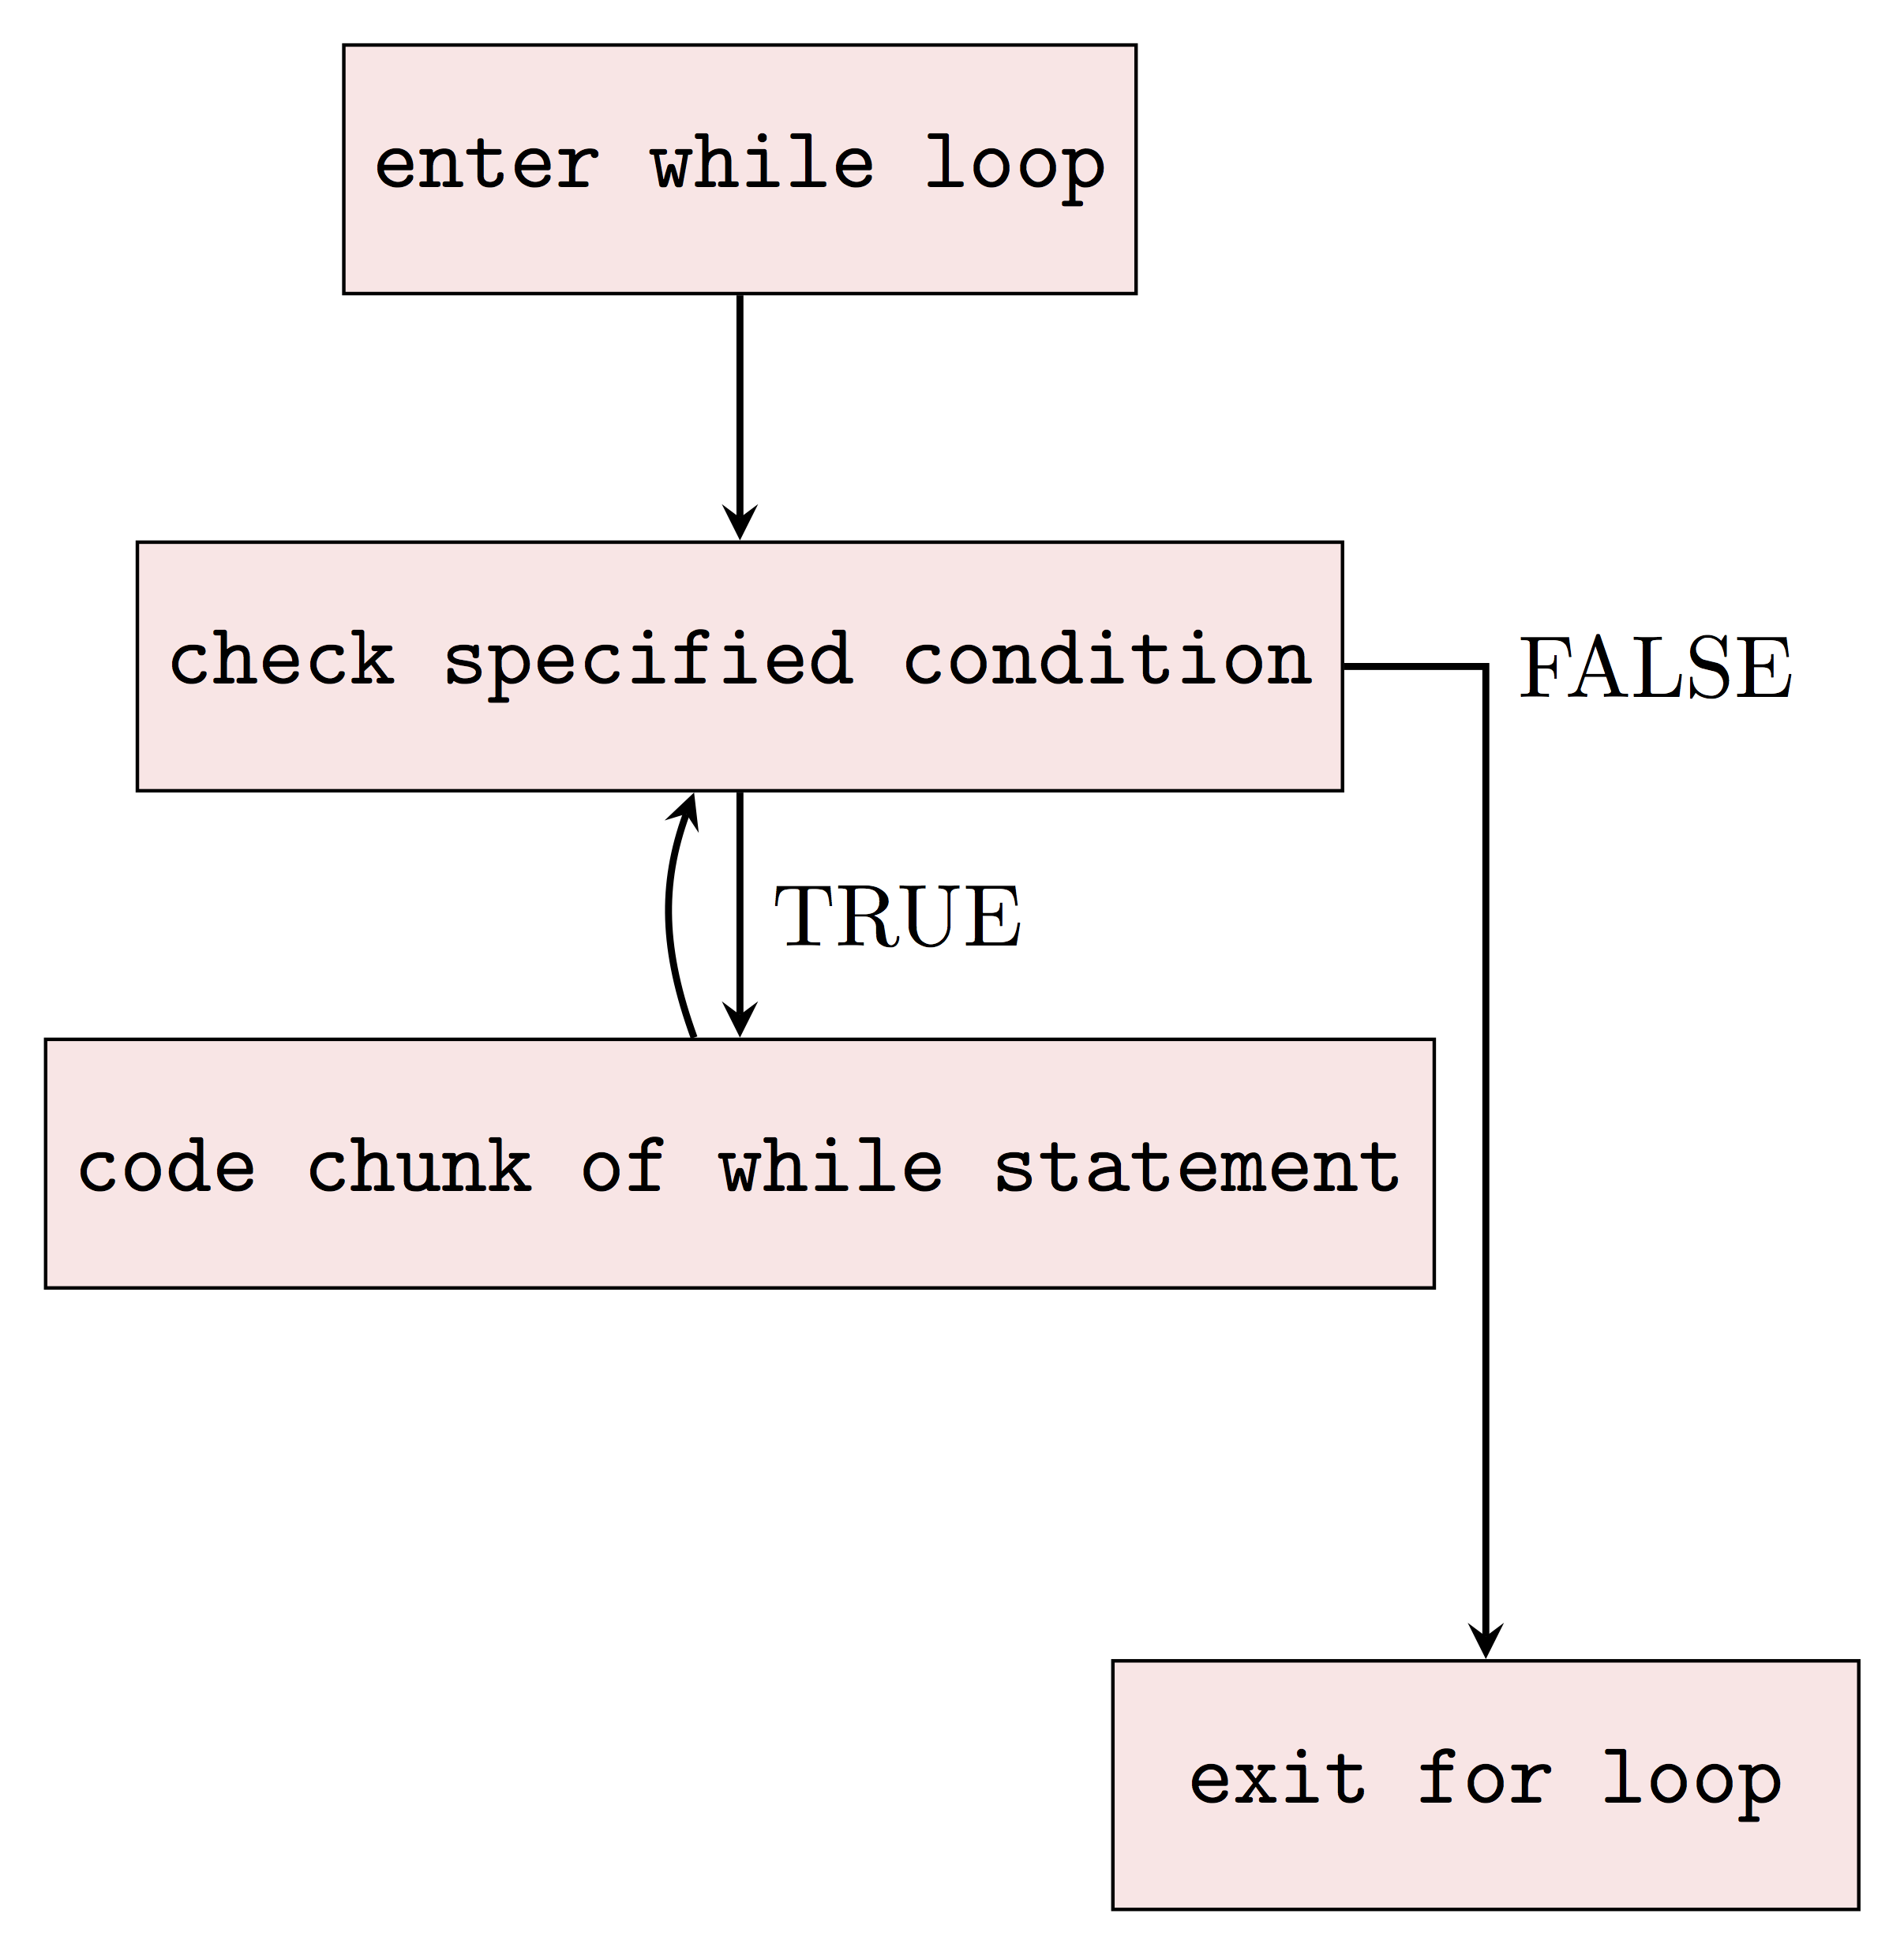
\includegraphics{images/flowchart___while_statement.png}

\section{Example: The Bootstrap}\label{example-the-bootstrap}

The (non-parametric) bootstrap was introduced by
\citet{efron1979bootstrap} as a numerical method to provide a simple
estimator of the distribution of an estimator. This method became
rapidly very popular since it is completely automatic, requires no
theoretical derivation and is (almost) always available no matter how
complicated our estimator of interest is. Moreover, most statistical
methods are based on various asymptotic approximations (often through
the central limit theorem) that can however deliver poor results in
finite sample settings. Bootstrap techniques generally enjoy better
finite sample performance while paying a price in terms of computation
burden. A formal discussion of the properties of (non-parametric)
bootstrap techniques is far beyond the scope of this textbook but it's
actually quite simple to understand its algorithm. To motivate this
discussion, suppose that we ask 10 students how much time they work at
home for their STAT 297 class. Say we obtain the following results (in
hours):

\begin{Shaded}
\begin{Highlighting}[]
\NormalTok{student_work <-}\StringTok{ }\KeywordTok{c}\NormalTok{(}\DecValTok{0}\NormalTok{, }\DecValTok{0}\NormalTok{, }\DecValTok{0}\NormalTok{, }\DecValTok{0}\NormalTok{, }\DecValTok{0}\NormalTok{, }\FloatTok{0.25}\NormalTok{, }\FloatTok{0.75}\NormalTok{, }\FloatTok{0.75}\NormalTok{, }\DecValTok{1}\NormalTok{, }\FloatTok{1.25}\NormalTok{, }\DecValTok{6}\NormalTok{)}
\end{Highlighting}
\end{Shaded}

We can compute the mean time spent

\begin{Shaded}
\begin{Highlighting}[]
\NormalTok{mean_hour <-}\StringTok{ }\KeywordTok{mean}\NormalTok{(student_work)}
\end{Highlighting}
\end{Shaded}

Moreover, we compute a simple confidence interval of the \textbf{average
number} of hours spent by a student enrolled in STAT 297. Since we have
no reason to believe that the number of hours spent working at home for
this class is not Gaussian, we can construct an asymtotic confidence
interval using:

\[
\bar{x} \pm z_{1-\alpha/2} \frac{\hat{\sigma}}{\sqrt{n}},
\]

where \(\bar{x}\) is the sample mean, \(\alpha\) is the significance
level which delivers \(z_{1-\alpha/2}\) quantile of standard Gaussian
distribution and \(\hat{\sigma}\) is the sample standard deviation (we
assume that estimating the standard deviation has no impact on the
distribution of \(\bar{x}\)). In R, this interval can therefore be
computed as follows:

\begin{Shaded}
\begin{Highlighting}[]
\NormalTok{alpha <-}\StringTok{ }\FloatTok{0.05}
\NormalTok{n <-}\StringTok{ }\KeywordTok{length}\NormalTok{(student_work)}
\NormalTok{sd_hour <-}\StringTok{ }\KeywordTok{sd}\NormalTok{(student_work)}
\NormalTok{z <-}\StringTok{ }\KeywordTok{qnorm}\NormalTok{(}\DecValTok{1} \OperatorTok{-}\StringTok{ }\NormalTok{alpha}\OperatorTok{/}\DecValTok{2}\NormalTok{)}
\NormalTok{mean_hour }\OperatorTok{+}\StringTok{ }\KeywordTok{c}\NormalTok{(}\OperatorTok{-}\DecValTok{1}\NormalTok{, }\DecValTok{1}\NormalTok{)}\OperatorTok{*}\NormalTok{z}\OperatorTok{*}\NormalTok{sd_hour}\OperatorTok{/}\KeywordTok{sqrt}\NormalTok{(n)}
\end{Highlighting}
\end{Shaded}

\begin{verbatim}
## [1] -0.1256494  1.9438313
\end{verbatim}

Based on this confidence interval your instructor is very disappointed
since the confidence interval includes 0, indicating that it is possible
that the students study on average zero hours. But does this interval
makes sense? The lower bound of the interval is negative implying that
students can also have negative hours of study. This of course makes no
sense indicating that with this sample size the asymptotic Gaussian
approximation makes little sense.

To solve this issue, the (non-parametric) bootstrap is a convenient and
appropriate tool to compute more adequate finite sample confidence
intervals. Letting
\(\mathbf{X} = \left[X_1 \;\; \ldots \;\; X_n\right]\) denote the sample
(in our case \texttt{student\_work}), the way the bootstrap works is as
follows:

\begin{itemize}
\tightlist
\item
  \textbf{Step 1:} Let \(i = 1\).
\item
  \textbf{Step 2:} Construct a new sample, say \(\mathbf{X}^*\), by
  sampling \textbf{with replacement} \(n\) observations from
  \(\mathbf{X}\).
\item
  \textbf{Step 3:} Compute the average of \(\mathbf{X}^*\) which we will
  denote as \(\bar{X}_i\). Let \(i = i + 1\) and if \(i < B\) go to
  \textbf{Step 2} otherwise go to \textbf{Step 4}.
\item
  \textbf{Step 4}: Compute the empirical quantiles of \(\bar{X}_i\).
\end{itemize}

Here is a simple function to implement this approach:

\begin{Shaded}
\begin{Highlighting}[]
\CommentTok{# Number of boostrap replications}
\NormalTok{B <-}\StringTok{ }\DecValTok{500}

\CommentTok{# Compute the length of vector}
\NormalTok{n <-}\StringTok{ }\KeywordTok{length}\NormalTok{(student_work)}

\CommentTok{# Confidence level}
\NormalTok{alpha <-}\StringTok{ }\FloatTok{0.05}

\CommentTok{# Initialisation of }
\NormalTok{boot_mean <-}\StringTok{ }\KeywordTok{rep}\NormalTok{(}\OtherTok{NA}\NormalTok{, B)}

\CommentTok{# Step 1}
\ControlFlowTok{for}\NormalTok{ (i }\ControlFlowTok{in} \DecValTok{1}\OperatorTok{:}\NormalTok{B)\{}
  \CommentTok{# Step 2}
\NormalTok{  student_work_star <-}\StringTok{ }\NormalTok{student_work[}\KeywordTok{sample}\NormalTok{(}\DecValTok{1}\OperatorTok{:}\NormalTok{n, }\DataTypeTok{replace =} \OtherTok{TRUE}\NormalTok{)]}
  
  \CommentTok{# Step 3}
\NormalTok{  boot_mean[i] <-}\StringTok{ }\KeywordTok{mean}\NormalTok{(student_work_star)}
\NormalTok{\}}

\CommentTok{# Step 4}
\KeywordTok{quantile}\NormalTok{(boot_mean, }\KeywordTok{c}\NormalTok{(alpha}\OperatorTok{/}\DecValTok{2}\NormalTok{, }\DecValTok{1} \OperatorTok{-}\StringTok{ }\NormalTok{alpha}\OperatorTok{/}\DecValTok{2}\NormalTok{))}
\end{Highlighting}
\end{Shaded}

\begin{verbatim}
##      2.5%     97.5% 
## 0.2045455 2.0801136
\end{verbatim}

Based on this result your instructor is relieved since they know that,
at a level of confidence of 95\%, you are spending at least more than 10
minutes on your course work.

\BeginKnitrBlock{rmdnote}
How would you modify the above code to obtain the same output using the
\texttt{while} control?
\EndKnitrBlock{rmdnote}

\BeginKnitrBlock{rmdnote}
A researcher developed a new drug to help patients recover after a
surgery. To investigate if her drug is working as expected, she starts
by creating a simple test experiment on mice. In this experiment, the
researcher records the survival times of 14 mice after a test surgery.
Out of the 14 mice, 8 of them are given the new drug while the remaining
ones are used as a control group (where no treatement is given). Her
results (in days) are the following:

\begin{itemize}
\tightlist
\item
  \textbf{Treatement} group: 38, 76, 121, 86, 52, 69, 41 and 171;
\item
  \textbf{Control} group: 18, 12, 52, 82, 102 and 25.
\end{itemize}

She believes that the median survival time is a ``good'' way to measure
effectiveness of her drug. Based on this experiment, she obtains that
the median survival time for the control group is 38.5 days while it is
72.5 days for the treatement group. She wonders if you could help her to
find an approriate (bootstrap) confidence interval for the difference of
the medians. Using this result, do you believe that the drug increases
the median survial time of mice after the test surgery?
\EndKnitrBlock{rmdnote}

\section{Example: Random Walk}\label{example-random-walk}

The term \emph{random walk} was first introduced by Karl Pearson in the
early nineteen-hundreds. There exist a large range of random walk
processes. For example, one of the simplest forms of a random walk
process can be explained as follows: suppose that you are walking on
campus and your next step can either be to your left, your right,
forward or backward (each with equal probability). The code illustrates
how to program such a random process:

\begin{Shaded}
\begin{Highlighting}[]
\CommentTok{# Control seed}
\KeywordTok{set.seed}\NormalTok{(}\DecValTok{1992}\NormalTok{)}

\CommentTok{# Number of steps}
\NormalTok{steps <-}\StringTok{ }\DecValTok{10}\OperatorTok{^}\DecValTok{5}

\CommentTok{# Direction probability (i.e. all direction are equally likely)}
\NormalTok{probs <-}\StringTok{ }\KeywordTok{c}\NormalTok{(}\FloatTok{0.25}\NormalTok{, }\FloatTok{0.5}\NormalTok{, }\FloatTok{0.75}\NormalTok{)}

\CommentTok{# Initial matrix}
\NormalTok{step_direction <-}\StringTok{ }\KeywordTok{matrix}\NormalTok{(}\DecValTok{0}\NormalTok{, steps}\OperatorTok{+}\DecValTok{1}\NormalTok{, }\DecValTok{2}\NormalTok{)}

\CommentTok{# Start random walk}
\ControlFlowTok{for}\NormalTok{ (i }\ControlFlowTok{in} \KeywordTok{seq}\NormalTok{(}\DecValTok{2}\NormalTok{, steps}\OperatorTok{+}\DecValTok{1}\NormalTok{))\{}
  \CommentTok{# Draw a random number from U(0,1)}
\NormalTok{  rn =}\StringTok{ }\KeywordTok{runif}\NormalTok{(}\DecValTok{1}\NormalTok{)}

  \CommentTok{# Go right if rn \textbackslash{}in [0,prob[1])}
  \ControlFlowTok{if}\NormalTok{ (rn }\OperatorTok{<}\StringTok{ }\NormalTok{probs[}\DecValTok{1}\NormalTok{]) \{step_direction[i,}\DecValTok{1}\NormalTok{] =}\StringTok{ }\DecValTok{1}\NormalTok{\}}

  \CommentTok{# Go left if rn \textbackslash{}in [probs[1], probs[2])}
  \ControlFlowTok{if}\NormalTok{ (rn }\OperatorTok{>=}\StringTok{ }\NormalTok{probs[}\DecValTok{1}\NormalTok{] }\OperatorTok{&&}\StringTok{ }\NormalTok{rn }\OperatorTok{<}\StringTok{ }\NormalTok{probs[}\DecValTok{2}\NormalTok{]) \{step_direction[i,}\DecValTok{1}\NormalTok{] =}\StringTok{ }\OperatorTok{-}\DecValTok{1}\NormalTok{\}}

  \CommentTok{# Go forward if rn \textbackslash{}in [probs[2], probs[3])}
  \ControlFlowTok{if}\NormalTok{ (rn }\OperatorTok{>=}\StringTok{ }\NormalTok{probs[}\DecValTok{2}\NormalTok{] }\OperatorTok{&&}\StringTok{ }\NormalTok{rn }\OperatorTok{<}\StringTok{ }\NormalTok{probs[}\DecValTok{3}\NormalTok{]) \{step_direction[i,}\DecValTok{2}\NormalTok{] =}\StringTok{ }\DecValTok{1}\NormalTok{\}}

  \CommentTok{# Go backward if rn \textbackslash{}in [probs[3],1]}
  \ControlFlowTok{if}\NormalTok{ (rn }\OperatorTok{>=}\StringTok{ }\NormalTok{probs[}\DecValTok{3}\NormalTok{]) \{step_direction[i,}\DecValTok{2}\NormalTok{] =}\StringTok{ }\OperatorTok{-}\DecValTok{1}\NormalTok{\}}
\NormalTok{\}}

\CommentTok{# Cumulative steps}
\NormalTok{position =}\StringTok{ }\KeywordTok{data.frame}\NormalTok{(}\DataTypeTok{x =} \KeywordTok{cumsum}\NormalTok{(step_direction[, }\DecValTok{1}\NormalTok{]), }
                      \DataTypeTok{y =} \KeywordTok{cumsum}\NormalTok{(step_direction[, }\DecValTok{2}\NormalTok{]))}
  
\CommentTok{# Let's make a nice graph...}
\CommentTok{# Graph parameters}
\NormalTok{color =}\StringTok{ "blue4"}
\NormalTok{xlab =}\StringTok{ "X-position"}
\NormalTok{ylab =}\StringTok{ "Y-position"}
\NormalTok{pt_pch =}\StringTok{ }\DecValTok{16}
\NormalTok{pt.cex =}\StringTok{ }\DecValTok{2}
\NormalTok{main =}\StringTok{ }\KeywordTok{paste}\NormalTok{(}\StringTok{"Simulated 2D RW with"}\NormalTok{, steps, }\StringTok{"steps"}\NormalTok{, }\DataTypeTok{sep =} \StringTok{" "}\NormalTok{)}
\NormalTok{hues =}\StringTok{ }\KeywordTok{seq}\NormalTok{(}\DecValTok{15}\NormalTok{, }\DecValTok{375}\NormalTok{, }\DataTypeTok{length =} \DecValTok{3}\NormalTok{)}
\NormalTok{pt_col =}\StringTok{ }\KeywordTok{hcl}\NormalTok{(}\DataTypeTok{h =}\NormalTok{ hues, }\DataTypeTok{l =} \DecValTok{65}\NormalTok{, }\DataTypeTok{c =} \DecValTok{100}\NormalTok{)[}\DecValTok{1}\OperatorTok{:}\DecValTok{2}\NormalTok{]}
\KeywordTok{par}\NormalTok{(}\DataTypeTok{mar =} \KeywordTok{c}\NormalTok{(}\FloatTok{5.1}\NormalTok{, }\FloatTok{5.1}\NormalTok{, }\DecValTok{1}\NormalTok{, }\FloatTok{2.1}\NormalTok{))}

\CommentTok{# Main plot}
\KeywordTok{plot}\NormalTok{(}\OtherTok{NA}\NormalTok{,  }\DataTypeTok{xlim =} \KeywordTok{range}\NormalTok{(position[,}\DecValTok{1}\NormalTok{]), }
          \DataTypeTok{ylim =} \KeywordTok{range}\NormalTok{(}\KeywordTok{range}\NormalTok{(position[,}\DecValTok{2}\NormalTok{])), }
          \DataTypeTok{xlab =}\NormalTok{ xlab, }\DataTypeTok{ylab =}\NormalTok{ ylab, }\DataTypeTok{xaxt =} \StringTok{'n'}\NormalTok{, }
          \DataTypeTok{yaxt =} \StringTok{'n'}\NormalTok{, }\DataTypeTok{bty =} \StringTok{"n"}\NormalTok{, }\DataTypeTok{ann =} \OtherTok{FALSE}\NormalTok{)}
\NormalTok{win_dim =}\StringTok{ }\KeywordTok{par}\NormalTok{(}\StringTok{"usr"}\NormalTok{)}

\KeywordTok{par}\NormalTok{(}\DataTypeTok{new =} \OtherTok{TRUE}\NormalTok{)}
\KeywordTok{plot}\NormalTok{(}\OtherTok{NA}\NormalTok{, }\DataTypeTok{xlim =} \KeywordTok{range}\NormalTok{(position[,}\DecValTok{1}\NormalTok{]), }\DataTypeTok{ylim =} \KeywordTok{c}\NormalTok{(win_dim[}\DecValTok{3}\NormalTok{], win_dim[}\DecValTok{4}\NormalTok{] }\OperatorTok{+}\StringTok{ }\FloatTok{0.09}\OperatorTok{*}\NormalTok{(win_dim[}\DecValTok{4}\NormalTok{] }\OperatorTok{-}\StringTok{ }\NormalTok{win_dim[}\DecValTok{3}\NormalTok{])),}
       \DataTypeTok{xlab =}\NormalTok{ xlab, }\DataTypeTok{ylab =}\NormalTok{ ylab, }\DataTypeTok{xaxt =} \StringTok{'n'}\NormalTok{, }\DataTypeTok{yaxt =} \StringTok{'n'}\NormalTok{, }\DataTypeTok{bty =} \StringTok{"n"}\NormalTok{)}
\NormalTok{  win_dim =}\StringTok{ }\KeywordTok{par}\NormalTok{(}\StringTok{"usr"}\NormalTok{)}

\CommentTok{# Add grid}
\KeywordTok{grid}\NormalTok{(}\OtherTok{NULL}\NormalTok{, }\OtherTok{NULL}\NormalTok{, }\DataTypeTok{lty =} \DecValTok{1}\NormalTok{, }\DataTypeTok{col =} \StringTok{"grey95"}\NormalTok{)}

\CommentTok{# Add title}
\NormalTok{x_vec =}\StringTok{ }\KeywordTok{c}\NormalTok{(win_dim[}\DecValTok{1}\NormalTok{], win_dim[}\DecValTok{2}\NormalTok{], win_dim[}\DecValTok{2}\NormalTok{], win_dim[}\DecValTok{1}\NormalTok{])}
\NormalTok{y_vec =}\StringTok{ }\KeywordTok{c}\NormalTok{(win_dim[}\DecValTok{4}\NormalTok{], win_dim[}\DecValTok{4}\NormalTok{],}
\NormalTok{            win_dim[}\DecValTok{4}\NormalTok{] }\OperatorTok{-}\StringTok{ }\FloatTok{0.09}\OperatorTok{*}\NormalTok{(win_dim[}\DecValTok{4}\NormalTok{] }\OperatorTok{-}\StringTok{ }\NormalTok{win_dim[}\DecValTok{3}\NormalTok{]),}
\NormalTok{            win_dim[}\DecValTok{4}\NormalTok{] }\OperatorTok{-}\StringTok{ }\FloatTok{0.09}\OperatorTok{*}\NormalTok{(win_dim[}\DecValTok{4}\NormalTok{] }\OperatorTok{-}\StringTok{ }\NormalTok{win_dim[}\DecValTok{3}\NormalTok{]))}
\KeywordTok{polygon}\NormalTok{(x_vec, y_vec, }\DataTypeTok{col =} \StringTok{"grey95"}\NormalTok{, }\DataTypeTok{border =} \OtherTok{NA}\NormalTok{)}
\KeywordTok{text}\NormalTok{(}\DataTypeTok{x =} \KeywordTok{mean}\NormalTok{(}\KeywordTok{c}\NormalTok{(win_dim[}\DecValTok{1}\NormalTok{], win_dim[}\DecValTok{2}\NormalTok{])), }\DataTypeTok{y =}\NormalTok{ (win_dim[}\DecValTok{4}\NormalTok{] }\OperatorTok{-}\StringTok{ }\FloatTok{0.09}\OperatorTok{/}\DecValTok{2}\OperatorTok{*}\NormalTok{(win_dim[}\DecValTok{4}\NormalTok{] }\OperatorTok{-}\StringTok{ }\NormalTok{win_dim[}\DecValTok{3}\NormalTok{])), main)}

\CommentTok{# Add axes and box}
\KeywordTok{lines}\NormalTok{(x_vec[}\DecValTok{1}\OperatorTok{:}\DecValTok{2}\NormalTok{], }\KeywordTok{rep}\NormalTok{((win_dim[}\DecValTok{4}\NormalTok{] }\OperatorTok{-}\StringTok{ }\FloatTok{0.09}\OperatorTok{*}\NormalTok{(win_dim[}\DecValTok{4}\NormalTok{] }\OperatorTok{-}\StringTok{ }\NormalTok{win_dim[}\DecValTok{3}\NormalTok{])),}\DecValTok{2}\NormalTok{), }\DataTypeTok{col =} \DecValTok{1}\NormalTok{)}
\KeywordTok{box}\NormalTok{()}
\KeywordTok{axis}\NormalTok{(}\DecValTok{1}\NormalTok{, }\DataTypeTok{padj =} \FloatTok{0.3}\NormalTok{)}
\NormalTok{y_axis =}\StringTok{ }\KeywordTok{axis}\NormalTok{(}\DecValTok{2}\NormalTok{, }\DataTypeTok{labels =} \OtherTok{FALSE}\NormalTok{, }\DataTypeTok{tick =} \OtherTok{FALSE}\NormalTok{)}
\NormalTok{y_axis =}\StringTok{ }\NormalTok{y_axis[y_axis }\OperatorTok{<}\StringTok{ }\NormalTok{(win_dim[}\DecValTok{4}\NormalTok{] }\OperatorTok{-}\StringTok{ }\FloatTok{0.09}\OperatorTok{*}\NormalTok{(win_dim[}\DecValTok{4}\NormalTok{] }\OperatorTok{-}\StringTok{ }\NormalTok{win_dim[}\DecValTok{3}\NormalTok{]))]}
\KeywordTok{axis}\NormalTok{(}\DecValTok{2}\NormalTok{, }\DataTypeTok{padj =} \OperatorTok{-}\FloatTok{0.2}\NormalTok{, }\DataTypeTok{at =}\NormalTok{ y_axis)}

\CommentTok{# Add trajectory}
\KeywordTok{lines}\NormalTok{(position, }\DataTypeTok{type =} \StringTok{"l"}\NormalTok{, }\DataTypeTok{col =}\NormalTok{ color, }\DataTypeTok{pch =} \DecValTok{16}\NormalTok{)}
  
\CommentTok{# Start and end points}
\KeywordTok{points}\NormalTok{(}\KeywordTok{c}\NormalTok{(}\DecValTok{0}\NormalTok{,position[steps}\OperatorTok{+}\DecValTok{1}\NormalTok{,}\DecValTok{1}\NormalTok{]), }\KeywordTok{c}\NormalTok{(}\DecValTok{0}\NormalTok{,position[steps}\OperatorTok{+}\DecValTok{1}\NormalTok{,}\DecValTok{2}\NormalTok{]), }\DataTypeTok{cex =}\NormalTok{ pt.cex, }\DataTypeTok{col =}\NormalTok{ pt_col, }\DataTypeTok{pch =}\NormalTok{ pt_pch)}
  
\CommentTok{# Legend}
\NormalTok{leg_pos =}\StringTok{ }\KeywordTok{c}\NormalTok{(}\KeywordTok{min}\NormalTok{(position[,}\DecValTok{1}\NormalTok{]), }\KeywordTok{max}\NormalTok{(position[,}\DecValTok{2}\NormalTok{]))}
\KeywordTok{legend}\NormalTok{(leg_pos[}\DecValTok{1}\NormalTok{], leg_pos[}\DecValTok{2}\NormalTok{], }\KeywordTok{c}\NormalTok{(}\StringTok{"Start"}\NormalTok{,}\StringTok{"End"}\NormalTok{), }
      \DataTypeTok{col =}\NormalTok{ pt_col, }\DataTypeTok{pch =}\NormalTok{ pt_pch, }\DataTypeTok{pt.cex =}\NormalTok{ pt.cex, }\DataTypeTok{bty =} \StringTok{"n"}\NormalTok{)}
\end{Highlighting}
\end{Shaded}

\begin{center}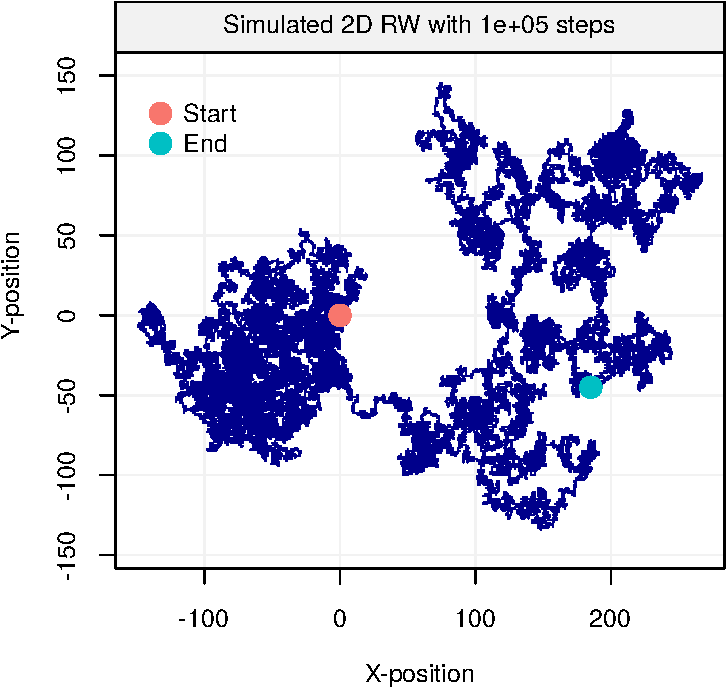
\includegraphics{ds_files/figure-latex/RW2d-1} \end{center}

Such processes inspired Karl Pearson's famous quote that

\begin{quote}
``\emph{the most likely place to find a drunken walker is somewhere near
his starting point.}''
\end{quote}

Empirical evidence of this phenomenon is not too hard to find on a
Friday night.

\section{Example: Monte-Carlo
Integration}\label{example-monte-carlo-integration}

\subsection{Introduction}\label{introduction-2}

Monte Carlo integration is a powerful technique for numerical
integration. It is particularly useful to evaluate integrals of
``high-dimension''. A detailed (and formal) discussion of this method is
clearly beyond the scope of this class and we shall restrict our
attention to the most basic form(s) of Monte Carlo integration and
briefly discuss the rational behind this method.

Originally, such Monte Carlo methods were known under various names
among which \emph{statistical sampling} was probably the most commonly
used. In fact, the name \emph{Monte Carlo} was popularized by several
researchers in Physics, including Stanislaw Ulam, Enrico Fermi and John
von Neumann. The name is believed to be a reference to a famous casino
in Monaco where Stanislaw Ulam's uncle would borrow money to gamble.
Enrico Fermi was one of the first to use this technique which he
employed to study the properties of a newly-discovered neutron in the
1930s. Later for example, these methods played a central role in many of
the simulations required for the Manhattan project.

With this in mind, let us give an idea of this approach by supposing we
are interested in computing the following integral:

\[I = \int_a^b f(x) dx.\]

Of course, this integral can be approximated by a Riemann sum:

\[I \approx \Delta x \sum_{i = 1}^n f(a + (i-1) \Delta x),\]

where \(\Delta x = \frac{b - a}{n}\;\) and the idea behind this
approximation is that as the number of partitions \(n\) increases, the
Riemann sum will become closer and closer to \(I\). Also (under some
technical conditions), we have that

\[I = \lim_{n \to \infty} \Delta x \sum_{i = 1}^n f(a + (i-1) \Delta x).\]

In fact, the rational of a Monte Carlo integral is quite close to the
Riemann sum since, in its most basic form, we approximate \(I\) by
averaging samples of the function \(f(x)\) at uniform random points
within the interval \([a, b]\). Therefore, the Monte Carlo
\emph{estimator} of \(I\) is given by

\begin{equation} 
\hat{I} = \frac{b - a}{B} \sum_{i = 1}^B f(X_i), 
 \label{eq:binom}
\end{equation}

where \(X_i = a + U_i (b - a)\) and \(U_i \sim \mathcal{U}(0,1)\). In
fact, \eqref{eq:binom} is quite intuitive since
\(\frac{1}{B} \sum_{i = 1}^B f(X_i)\) represents an estimation of the
average value of \(f(x)\) in the interval \([a, b]\) and thus
\(\hat{I}\) is simply the average value times the length of the
interval, i.e. \((b-a)\). If you would like to learn more about the
properties of Monte-Carlo integrals, click on the button below:

Properties

\hypertarget{hideclass1}{}
\BeginKnitrBlock{rmdnote}
A more formal argument on the validity of this approach can be found in
analyzing the statistical properties of the estimator \(\hat{I}\). In
order to do so, we start by considering its expected value \[
\mathbb{E}\left[ \hat{I} \right] = \frac{b - a}{B} \sum_{i = 1}^B \mathbb{E}\left[ f(X_i)  \right]
= \frac{b - a}{B} \sum_{i = 1}^B \int f(x) g(x) dx, 
\]

where \(g(x)\) denotes the pdf of \(X_i\). Since
\(X_i \sim \mathcal{U}(a, b)\) it follows that

\[
g(x) = \left\{
    \begin{array}{ll}
        \frac{1}{b - a}  & \mbox{if } x \in [a, b] \\
        0 & \mbox{if } x \not\in [a, b]
    \end{array}
\right.
\]

Therefore, we have

\[
\mathbb{E}\left[ \hat{I} \right] = \frac{b - a}{B} \sum_{i = 1}^B \int_a^b \frac{f(x)}{b-a} dx = \int_a^b f(x) dx = I, 
\]

Since \(X_i\) are iid, the same can be said about \(f(X_i)\) and
therefore by the \textbf{Strong Law of Large Numbers} we have that
\(\hat{I}\) converges \emph{almost surely} to \(I\), which means that

\[
\mathbb{P}\left(\lim_{B \to \infty} \hat{I} = I    \right) = 1.
\]

This result implies that as the number of simulations \(B\) goes to
infinity we can guarantee that the solution will be exact.

Unfortunately, this result doesn't give us any information on how
quickly this estimate converges to a ``sufficiently accurate'' solution
for the problem at hand. This can be done by studying the variance of
\(\hat{I}\) and its \emph{rate of convergence}. Indeed, we have

\[
\begin{aligned}
\operatorname{var} \left( \hat{I} \right) &= \left(\frac{b - a}{B}\right)^2  \sum_{i = 1}^B \left\{\mathbb{E}\left[f^2(X_i)\right] - \mathbb{E}^2\left[f(X_i)\right]\right\}\\
&= \frac{1}{B^2} \sum_{i = 1}^B \left\{(b-a) \int_a^b f^2(x) dx - \left(\int_a^b f(x) dx \right)^2 \right\}\\
&= \frac{(b-a) I_2 - I^2}{B}
\end{aligned}
\]

where \(I_2 = \int_a^b f^2(x) dx\). A simple estimator of this quantity
is given by

\[
\hat{I}_2 = \frac{b - a}{B} \sum_{i = 1}^B f^2(X_i),
\]

and therefore using \(\hat{I}\) we obtain:

\[
\widehat{\operatorname{var}} \left(\hat{I} \right) = \frac{(b-a) \hat{I}_2 - \hat{I}^2}{B} = \frac{b - a}{B^2} \sum_{i = 1}^B\left[ (b - a )f^2(X_i) - f(X_i)\right]
\]

Thus, it is easy to see that the rate of convergence of
\(\widehat{\operatorname{var}} \left(\hat{I} \right)\) is \(B^{-1}\) and
we may write
\({\operatorname{var}} \left(\hat{I} \right) = \mathcal{O}(B)\). This
implies that if we wish to reduce the error (or standard deviation) by
half, we need to quadruple \(B\). Such a phenomon is very common in many
fields of research such as Statistics where this is often called the
\emph{curse of dimensionality}.
\EndKnitrBlock{rmdnote}

\newline

\subsection{Implementation}\label{implementation}

The function \texttt{mc\_int()}, which is available in the
\texttt{stat297} package, implements the above method. This functions
has four inputs:

\begin{itemize}
\tightlist
\item
  \texttt{x\_range}: A vector containing the integration domain, i.e.
  \(a\) and \(b\),
\item
  \texttt{fun}: A string containing the function you wish to integrate
  where \(x\) is used to indicate the variable of integration,
\item
  \texttt{B}: A numeric value to denote the number of Monte-Carlo
  replications,
\item
  \texttt{seed}: A numeric value to control the seed of the random
  number generator.
\end{itemize}

For example, if you want to estimate

\[
\int_1^3 \frac{\exp\left(\sin(x)\right)}{x} dx,
\]

using \(10^4\) Monte-Carlo replications, you can use the following
command:

\begin{Shaded}
\begin{Highlighting}[]
\KeywordTok{library}\NormalTok{(stat297)}
\KeywordTok{mc_int}\NormalTok{(}\DataTypeTok{x_range =} \KeywordTok{c}\NormalTok{(}\DecValTok{1}\NormalTok{,}\DecValTok{3}\NormalTok{), }\DataTypeTok{fun =} \StringTok{"exp(sin(x))/x"}\NormalTok{, }\DataTypeTok{B =} \DecValTok{10}\OperatorTok{^}\DecValTok{5}\NormalTok{)}
\end{Highlighting}
\end{Shaded}

\begin{verbatim}
## $I
## [1] 2.558104
## 
## $var
## [1] 1.401222e-05
## 
## $fun
## [1] "exp(sin(x))/x"
## 
## $x_range
## [1] 1 3
## 
## $B
## [1] 1e+05
## 
## attr(,"class")
## [1] "MCI"
\end{verbatim}

At this point, it is probably a good idea to try to programm this
yourself and to compare your results (and code!) with the function
\texttt{mc\_int()}. This should be rather easy to implement but one
thing that may be a little delicate is how to pass the function you wish
to integrate as an input. A possible way of doing this is to use a
string so that, for example, if we have to integrate the function
\(\sin(x)\) you could simply write \texttt{fun\ =\ sin(x)} when calling
your function. This implies that we should be able to ``transform'' a
string into a function that we can evaluate, which is something that we
can achieve by combining the functions \texttt{eval} and \texttt{parse}.
An example is provided below:

\begin{Shaded}
\begin{Highlighting}[]
\NormalTok{my_fun =}\StringTok{ "x^2"}
\NormalTok{x =}\StringTok{ }\DecValTok{0}\OperatorTok{:}\DecValTok{3}
\KeywordTok{eval}\NormalTok{(}\KeywordTok{parse}\NormalTok{(}\DataTypeTok{text =}\NormalTok{ my_fun))}
\end{Highlighting}
\end{Shaded}

\begin{verbatim}
## [1] 0 1 4 9
\end{verbatim}

If you're having trouble understanding what these functions are doing
have a look at their help files by writing \texttt{?eval} and
\texttt{?parse}.

\subsection{Application to the Normal
Distribution}\label{application-to-the-normal-distribution}

Suppose that \(X \sim \mathcal{N}(4, 1.25^2)\) and that we are
interested in computing the following probability
\(\mathbb{P}\left(1 < X < 4.5 \right)\). The probability density of the
normal distribution for a random variable with mean \(\mu\) and variance
\(\sigma^2\) is given by:

\[
f(x) = \frac{1}{\sqrt{2 \pi \sigma^2}} \exp \left(- \frac{\left(x - \mu\right)^2}{2 \sigma^2}\right).
\]

Therefore, the probability we are interested in can be written as the
following integral

\[
\mathbb{P}\left(1 < X < 4.5 \right) = \int_1^{4.5} \frac{1}{\sqrt{3.125 \pi}} \exp \left(- \frac{\left(x - 4\right)^2}{3.125}\right).
\]

Analytically, this is not an easy problem and of course there are many
ways to solve it. However, we could try to use a Monte-Carlo integral to
solve it. For example:

\begin{Shaded}
\begin{Highlighting}[]
\NormalTok{my_fun =}\StringTok{ "1/sqrt(3.125*pi)*exp(-((x - 4)^2)/3.125)"}
\NormalTok{(}\DataTypeTok{prob =} \KeywordTok{mc_int}\NormalTok{(}\DataTypeTok{x_range =} \KeywordTok{c}\NormalTok{(}\DecValTok{1}\NormalTok{, }\FloatTok{4.5}\NormalTok{), }\DataTypeTok{fun =}\NormalTok{ my_fun, }\DataTypeTok{B =} \DecValTok{10}\OperatorTok{^}\DecValTok{7}\NormalTok{))}
\end{Highlighting}
\end{Shaded}

\begin{verbatim}
## $I
## [1] 0.6471691
## 
## $var
## [1] 1.449985e-08
## 
## $fun
## [1] "1/sqrt(3.125*pi)*exp(-((x - 4)^2)/3.125)"
## 
## $x_range
## [1] 1.0 4.5
## 
## $B
## [1] 1e+07
## 
## attr(,"class")
## [1] "MCI"
\end{verbatim}

Based on this result, we can write
\(\mathbb{P}\left(1 < X < 4.5 \right) \approx 64.72 \%\) with a standard
error of about 0.01\%. We can compare our results with what we would
obtain with the function \texttt{pnorm} which provides a nearly exact
result:

\begin{Shaded}
\begin{Highlighting}[]
\KeywordTok{pnorm}\NormalTok{(}\FloatTok{4.5}\NormalTok{, }\DecValTok{4}\NormalTok{, }\FloatTok{1.25}\NormalTok{) }\OperatorTok{-}\StringTok{ }\KeywordTok{pnorm}\NormalTok{(}\DecValTok{1}\NormalTok{, }\DecValTok{4}\NormalTok{, }\FloatTok{1.25}\NormalTok{)}
\end{Highlighting}
\end{Shaded}

\begin{verbatim}
## [1] 0.6472242
\end{verbatim}

This shows that our estimation is within one standard error of a near
perfect result.

\subsection{Application to Nonelementary
Integrals}\label{application-to-nonelementary-integrals}

In layman's terms, a nonelementary integral of a given (elementary)
function is an integral that cannot be expressed as an elementary
function. The French mathematicien Joseph Liouville was the first to
prove the existance of such a nonelementary integral. A well-known
example of such integrals are the Fresnel integrals that have been used
for a very wide range of applications going from the computation of
electromagnetic field intensity to roller roster design. These integrals
are defined as:

\[S(y) = \int_0^t \sin\left(x^2\right) dx \;\;\;\;\;\; \text{and}  \;\;\;\;\;\; 
C(y) = \int_0^y \cos \left( x^2 \right) dx.\]

In this example, we will only consider \(S(y)\). In general it is
believed that the most convenient way of evaluating these functions up
to an arbitrary level of precision is to use a power series
representation that converges for all \(y\):

\[
S(y) = \sum_{i = 1}^\infty \, \left(-1\right)^n \, \frac{y^{4i + 1}}{\left(2i + 1\right) \, !\left(4i + 3\right)}.
\]

In this example, we will study the estimation of \(S(\pi)\) as well as
the \emph{precision} of this estimation.

\begin{Shaded}
\begin{Highlighting}[]
\NormalTok{B =}\StringTok{ }\DecValTok{4}\OperatorTok{^}\NormalTok{(}\DecValTok{4}\OperatorTok{:}\DecValTok{13}\NormalTok{)}
\NormalTok{results =}\StringTok{ }\KeywordTok{matrix}\NormalTok{(}\OtherTok{NA}\NormalTok{, }\KeywordTok{length}\NormalTok{(B), }\DecValTok{2}\NormalTok{)}
\ControlFlowTok{for}\NormalTok{ (i }\ControlFlowTok{in} \DecValTok{1}\OperatorTok{:}\KeywordTok{length}\NormalTok{(B))\{}
\NormalTok{  mc_res =}\StringTok{ }\KeywordTok{mc_int}\NormalTok{(}\KeywordTok{c}\NormalTok{(}\DecValTok{0}\NormalTok{, }\DecValTok{2}\NormalTok{), }\StringTok{"sin(x^2)"}\NormalTok{, }\DataTypeTok{B =}\NormalTok{ B[i], }\DataTypeTok{seed =}\NormalTok{ i}\OperatorTok{+}\DecValTok{12}\NormalTok{)}
\NormalTok{  results[i, ] =}\StringTok{ }\KeywordTok{c}\NormalTok{(mc_res}\OperatorTok{$}\NormalTok{I, }\KeywordTok{sqrt}\NormalTok{(mc_res}\OperatorTok{$}\NormalTok{var))}
\NormalTok{\}}


\NormalTok{trans_blue =}\StringTok{ }\KeywordTok{hcl}\NormalTok{(}\DataTypeTok{h =} \KeywordTok{seq}\NormalTok{(}\DecValTok{15}\NormalTok{, }\DecValTok{375}\NormalTok{, }\DataTypeTok{length =} \DecValTok{3}\NormalTok{), }\DataTypeTok{l =} \DecValTok{65}\NormalTok{, }\DataTypeTok{c =} \DecValTok{100}\NormalTok{, }\DataTypeTok{alpha =} \FloatTok{0.15}\NormalTok{)[}\DecValTok{2}\NormalTok{]}
\KeywordTok{plot}\NormalTok{(}\OtherTok{NA}\NormalTok{, }\DataTypeTok{xlim =} \KeywordTok{range}\NormalTok{(B), }\DataTypeTok{ylim =} \KeywordTok{range}\NormalTok{(}\KeywordTok{cbind}\NormalTok{(results[, }\DecValTok{1}\NormalTok{] }\OperatorTok{+}\StringTok{ }\NormalTok{results[,}\DecValTok{2}\NormalTok{], }
\NormalTok{      results[, }\DecValTok{1}\NormalTok{] }\OperatorTok{-}\NormalTok{results[,}\DecValTok{2}\NormalTok{])), }\DataTypeTok{log =} \StringTok{"x"}\NormalTok{, }\DataTypeTok{ylab =} \StringTok{"Estimated Integral"}\NormalTok{,}
      \DataTypeTok{xlab =} \StringTok{"Number of Simulations B"}\NormalTok{, }\DataTypeTok{xaxt =} \StringTok{'n'}\NormalTok{)}
\KeywordTok{grid}\NormalTok{()}
\KeywordTok{axis}\NormalTok{(}\DecValTok{1}\NormalTok{, }\DataTypeTok{at =}\NormalTok{ B, }\DataTypeTok{labels =} \KeywordTok{parse}\NormalTok{(}\DataTypeTok{text =} \KeywordTok{paste}\NormalTok{(}\StringTok{"4^"}\NormalTok{, }\DecValTok{4}\OperatorTok{:}\DecValTok{13}\NormalTok{, }\DataTypeTok{sep =} \StringTok{""}\NormalTok{)))}
\KeywordTok{polygon}\NormalTok{(}\KeywordTok{c}\NormalTok{(B, }\KeywordTok{rev}\NormalTok{(B)), }\KeywordTok{c}\NormalTok{(results[, }\DecValTok{1}\NormalTok{] }\OperatorTok{+}\StringTok{ }\NormalTok{results[, }\DecValTok{2}\NormalTok{], }
                        \KeywordTok{rev}\NormalTok{(results[, }\DecValTok{1}\NormalTok{] }\OperatorTok{-}\StringTok{ }\NormalTok{results[, }\DecValTok{2}\NormalTok{])), }\DataTypeTok{border =} \OtherTok{NA}\NormalTok{, }\DataTypeTok{col =}\NormalTok{ trans_blue)}
\KeywordTok{lines}\NormalTok{(B, results[, }\DecValTok{1}\NormalTok{], }\DataTypeTok{type =} \StringTok{"b"}\NormalTok{, }\DataTypeTok{col =} \StringTok{"blue4"}\NormalTok{, }\DataTypeTok{pch =} \DecValTok{16}\NormalTok{)}
\KeywordTok{abline}\NormalTok{(}\DataTypeTok{h =} \FloatTok{0.8048208}\NormalTok{, }\DataTypeTok{col =} \StringTok{"red4"}\NormalTok{, }\DataTypeTok{lty =} \DecValTok{2}\NormalTok{)}
\KeywordTok{legend}\NormalTok{(}\StringTok{"topright"}\NormalTok{, }\KeywordTok{c}\NormalTok{(}\StringTok{"Estimated value"}\NormalTok{, }\StringTok{"Standard error interval"}\NormalTok{, }\StringTok{"Good approximation (MatLab)"}\NormalTok{), }\DataTypeTok{bty =} \StringTok{"n"}\NormalTok{,}
       \DataTypeTok{pch =} \KeywordTok{c}\NormalTok{(}\DecValTok{16}\NormalTok{, }\DecValTok{15}\NormalTok{, }\OtherTok{NA}\NormalTok{), }\DataTypeTok{lwd =} \KeywordTok{c}\NormalTok{(}\DecValTok{1}\NormalTok{, }\OtherTok{NA}\NormalTok{, }\DecValTok{1}\NormalTok{), }\DataTypeTok{lty =} \KeywordTok{c}\NormalTok{(}\DecValTok{1}\NormalTok{, }\OtherTok{NA}\NormalTok{, }\DecValTok{2}\NormalTok{), }
       \DataTypeTok{pt.cex =} \KeywordTok{c}\NormalTok{(}\DecValTok{1}\NormalTok{, }\DecValTok{2}\NormalTok{, }\OtherTok{NA}\NormalTok{), }\DataTypeTok{col =} \KeywordTok{c}\NormalTok{(}\StringTok{"blue4"}\NormalTok{, trans_blue, }\StringTok{"red4"}\NormalTok{))}
\end{Highlighting}
\end{Shaded}

\begin{center}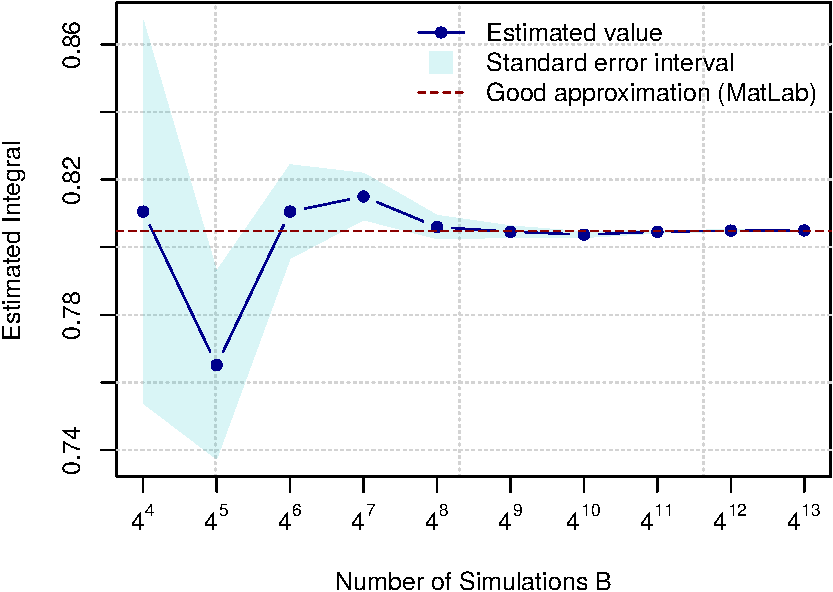
\includegraphics{ds_files/figure-latex/unnamed-chunk-170-1} \end{center}

\chapter{Functions}\label{functions}

This chapter aims at highlighting the main advantages, characteristics,
arguments and structure of functions in R. As you might already know, a
function is a collection of logically connected commands and operations
that allow the user to input some arguments and obtain a desired output
(based on the given arguments) without having to rewrite the mentioned
code each time that specific output is needed. Indeed, a common task in
statistical research for example consists in running some simulation
studies which give support (or not) to the use of a certain method of
inference. In this case, it's not efficient to rewrite the code each
time it is needed within a simulation study because it would lead to
lengthy code and increased risk of miss-coding.

In the following paragraphs, we will describe an example for which we
will build a function that allows to respond to the related research
question. Following from the previous chapter where we discussed matrix
algebra in R, at the end of this chapter we will therefore implement a
function that allows us to perform least-squares regression and
inference using these notions of matrix algebra. Indeed, it may be
interesting to understand the behavior of this estimator in different
simulation settings and it would not be practical to rewrite the series
of commands to obtain the least-squares estimator in each setting. For
this reason, a function that implements this estimator would be more
appropriate and, in fact, this function already exists in the base R
functions and is called \texttt{lm()}. However, we will learn how to
build our own least-squares regression function and compare its results
with those of \texttt{lm()} to check if they're the same. To do so, we
will consider a dataset in which linear regression is used to study the
age of the universe.

\textbf{Example: The Hubble Constant}

The example dataset we will study is taken from
\citet{wood2017generalized} which discusses data collected from the
Hubble Space Telescope key project containing information on the
velocity and relative distance of 24 galaxies. This information has been
used to compute the ``Hubble constant'' which is a fixed parameter that
links velocity and distance of celestial bodies through which it is
possible to compute the age of the universe based on the ``Big Bang''
theory. The link is given by this simple linear relationship

\begin{equation*}
  y = \beta x ,
\end{equation*}

where \(y\) represents the velocity while \(x\) is the distance between
galaxies. Once the Hubble constant is known, its inverse (i.e.
\(\beta^{-1}\)) gives the age of the universe based on the big bang
theory.

Therefore we will use the abovementioned dataset to estimate Hubble's
constant to then get an estimate of the age of the universe. This
dataset can be found in the \texttt{gamair} package under the name
\texttt{hubble} and when plotting the two variables of interest in a
scatterplot there appears to be a positive linear relationship between
the two variables.

\begin{Shaded}
\begin{Highlighting}[]
\CommentTok{# Load gamair library and retrieve Hubble dataset}
\KeywordTok{library}\NormalTok{(gamair)}
\end{Highlighting}
\end{Shaded}

\begin{verbatim}
## Error in library(gamair): there is no package called 'gamair'
\end{verbatim}

\begin{Shaded}
\begin{Highlighting}[]
\KeywordTok{data}\NormalTok{(hubble)}
\end{Highlighting}
\end{Shaded}

\begin{verbatim}
## Warning in data(hubble): data set 'hubble' not found
\end{verbatim}

\begin{Shaded}
\begin{Highlighting}[]
\CommentTok{# Plot data}
\KeywordTok{plot}\NormalTok{(}\DataTypeTok{y =}\NormalTok{ hubble}\OperatorTok{$}\NormalTok{y, }\DataTypeTok{x =}\NormalTok{ hubble}\OperatorTok{$}\NormalTok{x, }\DataTypeTok{col=}\StringTok{"darkblue"}\NormalTok{, }\DataTypeTok{pch =} \DecValTok{20}\NormalTok{, }\DataTypeTok{main=}\StringTok{"Distance vs. Velocity"}\NormalTok{, }
     \DataTypeTok{ylab =} \StringTok{"Velocity (in km/s)"}\NormalTok{, }\DataTypeTok{xlab =} \StringTok{"Distance (in Megaparsecs)"}\NormalTok{)}
\end{Highlighting}
\end{Shaded}

\begin{verbatim}
## Error in plot(y = hubble$y, x = hubble$x, col = "darkblue", pch = 20, : object 'hubble' not found
\end{verbatim}

\begin{Shaded}
\begin{Highlighting}[]
\KeywordTok{grid}\NormalTok{()}
\end{Highlighting}
\end{Shaded}

\begin{verbatim}
## Error in int_abline(a = a, b = b, h = h, v = v, untf = untf, ...): plot.new has not been called yet
\end{verbatim}

By the end of this chapter we will therefore be able to build a function
to obtain an estimate of \(\beta\) and, consequently, an estimate of the
age of the universe based on the big bang theory (as well as a means of
testing whether a Creationist hypothesis on the age of the universe is
reasonable based on the latter theory).

\section{R functions}\label{r-functions}

In order to build our own functions, the next sections will present the
main features of functions in R by studying their main components. The
following annotated example gives a brief overview of a simple function
that draws a random number issued from the ``spin'' of an American
roulette \footnote{This scheme is inspired from diagrams by Prof.~Bob
  Rudis and James Balamuta.}:

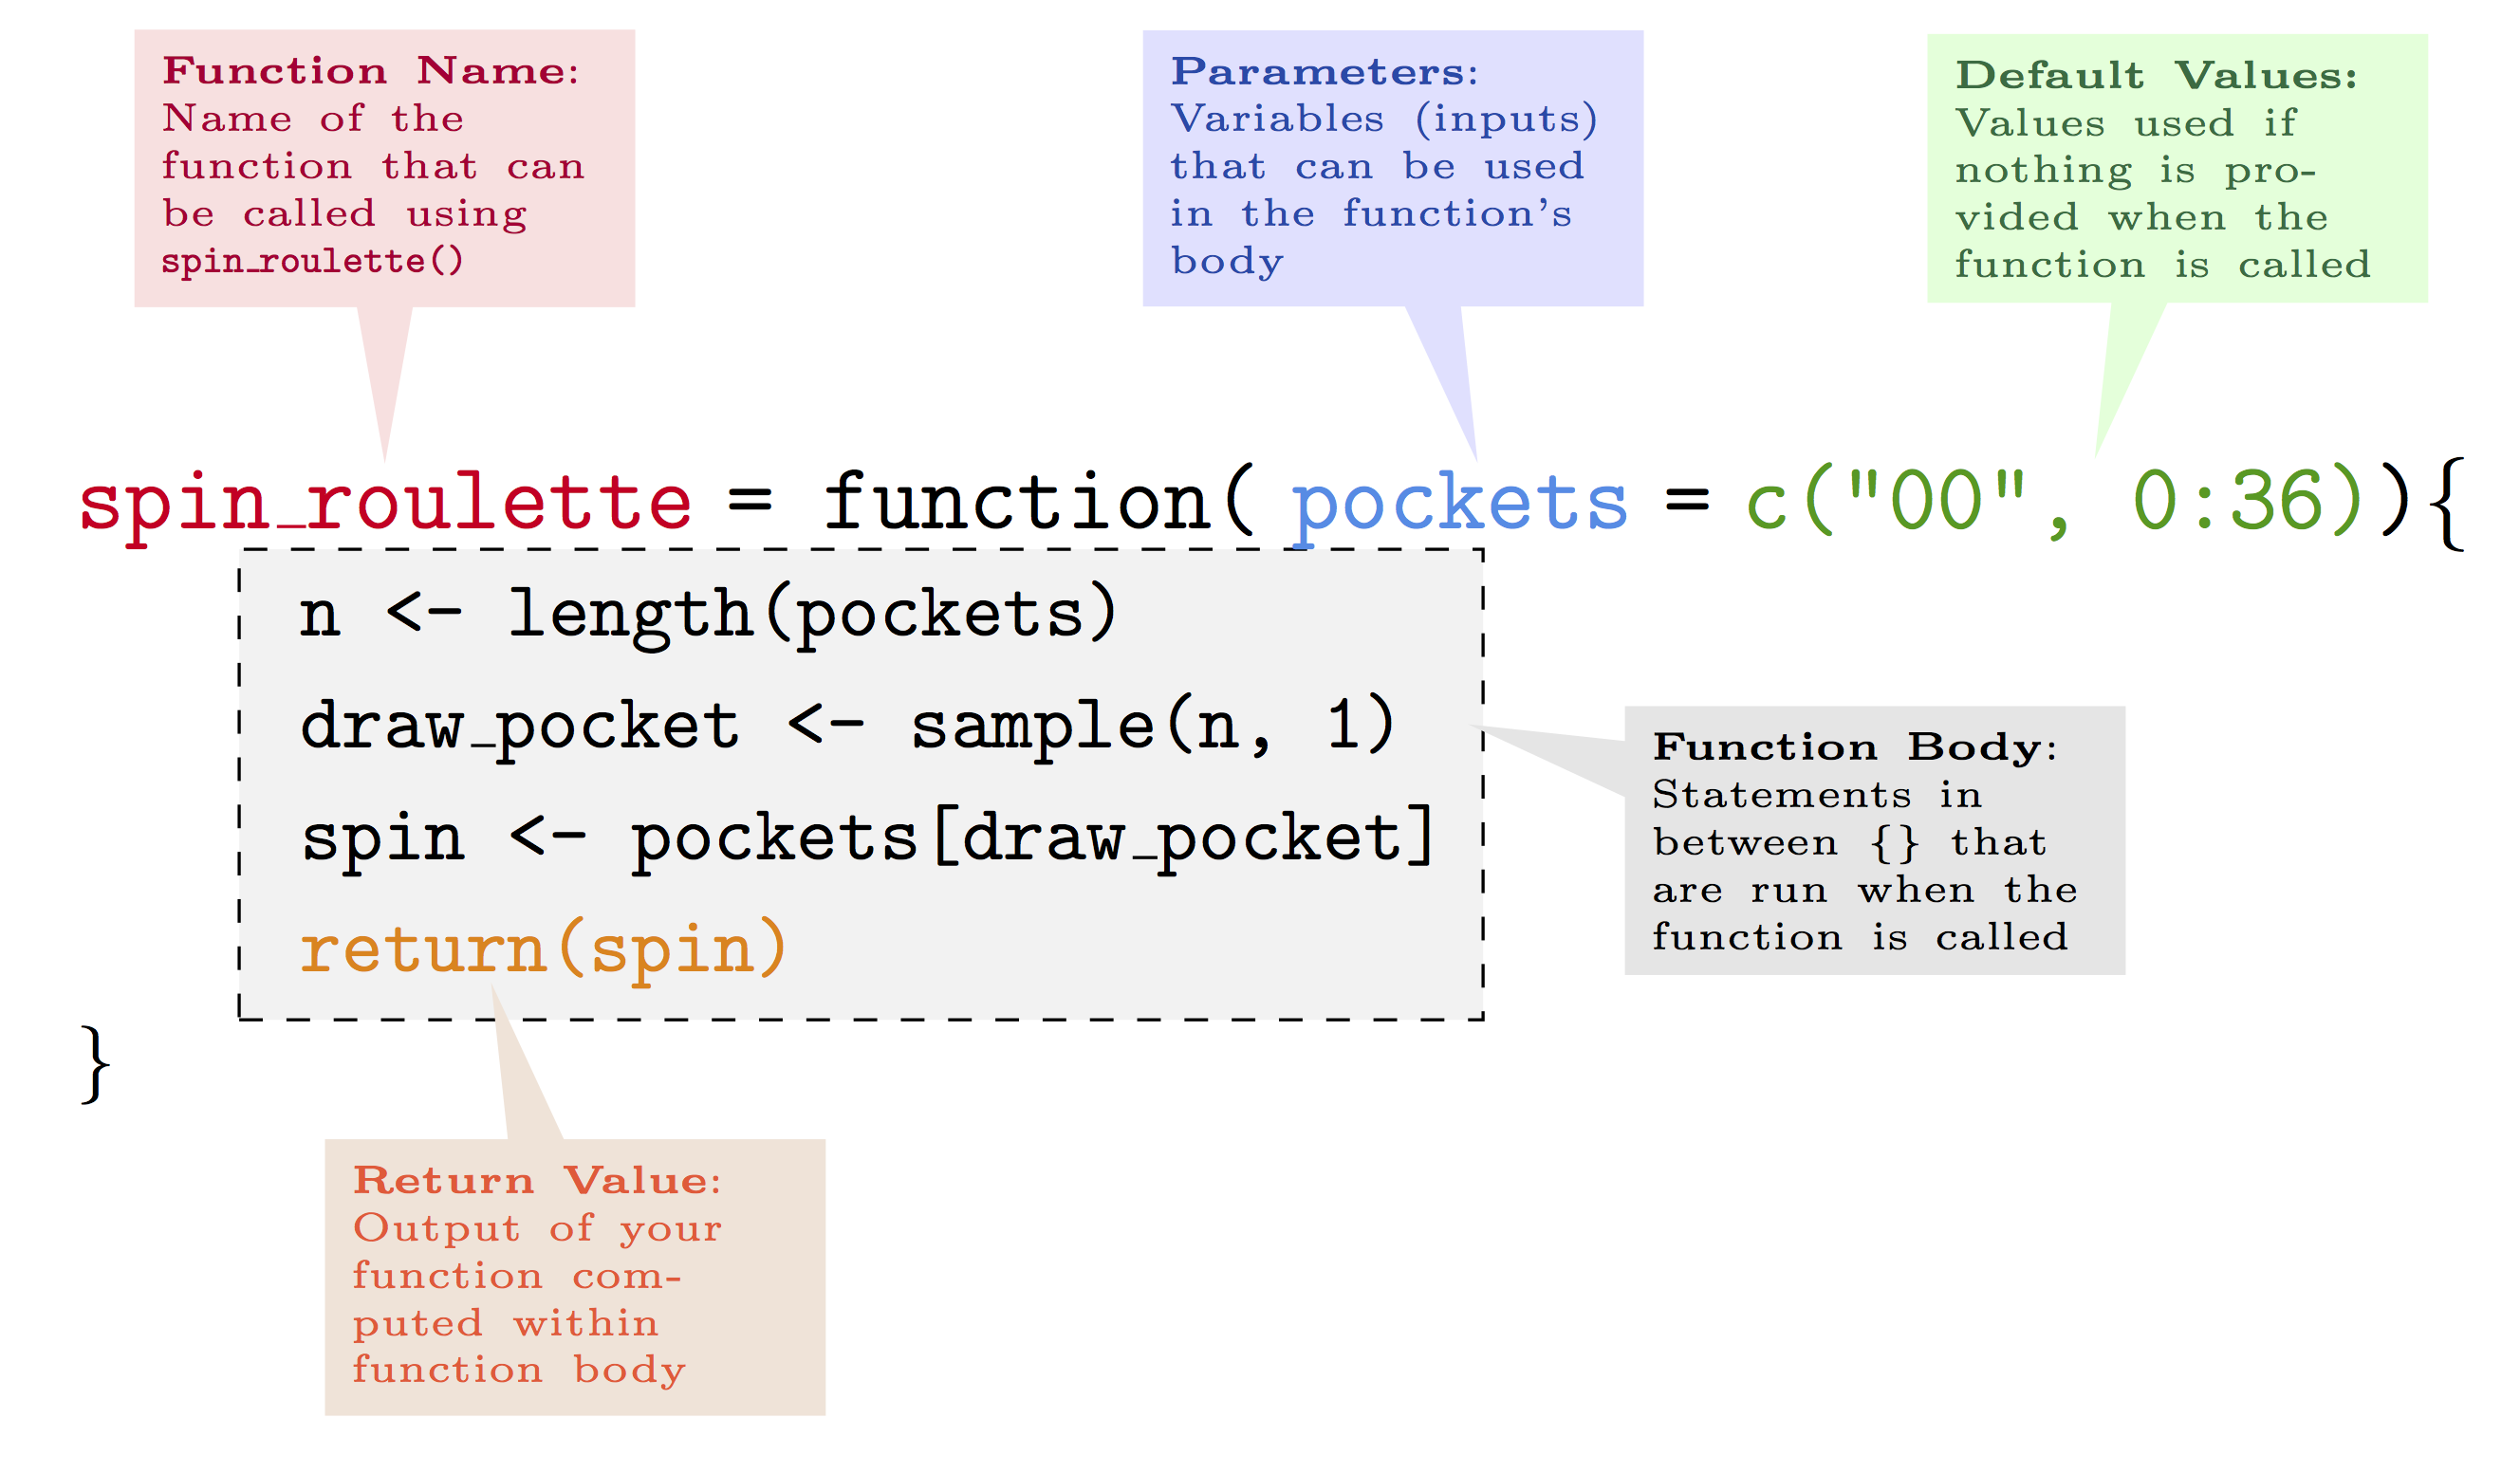
\includegraphics[width=0.80000\textwidth]{images/function.png}

As can be noticed, we first define the name we want to give to the
function.

\BeginKnitrBlock{rmdwarning}
It is important to make sure that the function name is specific and does
not correspond to other functions that may need to be used within your
work session. If two functions have the same name, just as with other R
objects, the function that will be used is the last one that has been
defined within the R working session.
\EndKnitrBlock{rmdwarning}

Once we have defined the name, we then attribute a function to this name
by using the \texttt{function} syntax to which we assign some parameters
(or attributes). The latter are the values or data that the user will
input in order for the function to deliver the desired output. The
latter is subsequently obtained through the code constituting the
\emph{body} of the function. Once the code has made the necessary
computations, the function needs to know which results are to be given
as an output. This can be done, for example, using the \texttt{return}
syntax.

A couple of simple examples can be functions that compute the sample
mean:

\begin{Shaded}
\begin{Highlighting}[]
\NormalTok{my_mean <-}\StringTok{ }\ControlFlowTok{function}\NormalTok{ (x) \{}
\NormalTok{  average <-}\StringTok{ }\KeywordTok{sum}\NormalTok{(x, }\DataTypeTok{na.rm =}\NormalTok{ T)}\OperatorTok{/}\KeywordTok{sum}\NormalTok{(}\OperatorTok{!}\KeywordTok{is.na}\NormalTok{(x))}
  \KeywordTok{return}\NormalTok{(average)}
\NormalTok{\}}
\end{Highlighting}
\end{Shaded}

or multiplies two numbers:

\begin{Shaded}
\begin{Highlighting}[]
\NormalTok{my_prod <-}\StringTok{ }\ControlFlowTok{function}\NormalTok{ (a, b) \{}
\NormalTok{  prod <-}\StringTok{ }\NormalTok{a}\OperatorTok{*}\NormalTok{b}
  \KeywordTok{return}\NormalTok{(prod)}
\NormalTok{\}}
\end{Highlighting}
\end{Shaded}

Using these functions, we can compute the sample mean of the annual
precipitation in US cities (that can be found in the base R dataset
\texttt{precip}):

\begin{Shaded}
\begin{Highlighting}[]
\KeywordTok{my_mean}\NormalTok{(precip)}
\end{Highlighting}
\end{Shaded}

\begin{verbatim}
## [1] 34.88571
\end{verbatim}

or the product of 265 and 83:

\begin{Shaded}
\begin{Highlighting}[]
\KeywordTok{my_prod}\NormalTok{(}\DecValTok{265}\NormalTok{, }\DecValTok{83}\NormalTok{)}
\end{Highlighting}
\end{Shaded}

\begin{verbatim}
## [1] 21995
\end{verbatim}

A particular case of function building are so-called ``infix'' functions
that allow to create new operators that carry out specific types of
computations. So, instead of defining the name of a function, you can
define the symbol to be used in order to make use of that function. For
example, to sum two numbers in R you can do as follows:

\begin{Shaded}
\begin{Highlighting}[]
\DecValTok{1} \OperatorTok{+}\StringTok{ }\DecValTok{2}
\end{Highlighting}
\end{Shaded}

\begin{verbatim}
## [1] 3
\end{verbatim}

which is simply a predefined infix function that can also be used as
follows:

\begin{Shaded}
\begin{Highlighting}[]
\StringTok{`}\DataTypeTok{+}\StringTok{`}\NormalTok{(}\DecValTok{1}\NormalTok{, }\DecValTok{2}\NormalTok{)}
\end{Highlighting}
\end{Shaded}

\begin{verbatim}
## [1] 3
\end{verbatim}

Therefore the \texttt{+} operator is the result of a predefined infix
function in R. However, all user-defined infix functions must start and
end with the \texttt{\%} symbol. For example, using an operator that we
define as \texttt{\%\^{}\%}, we can deliver the product of two numbers
that is zero if the product is actually negative:

\begin{Shaded}
\begin{Highlighting}[]
\StringTok{`}\DataTypeTok\StringTok{`}\NormalTok{ <-}\StringTok{ }\ControlFlowTok{function}\NormalTok{(a, b) \{}
\NormalTok{  prod =}\StringTok{ }\NormalTok{a}\OperatorTok{*}\NormalTok{b}
\NormalTok{  (prod }\OperatorTok{>}\StringTok{ }\DecValTok{0}\NormalTok{)}\OperatorTok{*}\NormalTok{prod}
\NormalTok{\}}
\end{Highlighting}
\end{Shaded}

This infix function can now be used through the operator as follows:

\begin{Shaded}
\begin{Highlighting}[]
\DecValTok{2} \OperatorTok\StringTok{ }\DecValTok{2}
\end{Highlighting}
\end{Shaded}

\begin{verbatim}
## [1] 4
\end{verbatim}

\begin{Shaded}
\begin{Highlighting}[]
\DecValTok{2} \OperatorTok\StringTok{ }\OperatorTok{-}\DecValTok{1}
\end{Highlighting}
\end{Shaded}

\begin{verbatim}
## [1] 0
\end{verbatim}

Having described the general structure of an R function, let us go more
into detail by analysing the three main components to R functions:

\begin{itemize}
\tightlist
\item
  \textbf{body}: the code lines containing the commands and operations
  which deliver the desired output;
\item
  \textbf{arguments}: the inputs the user gives to the function which
  will determine the value or type of output of a function;
\item
  \textbf{environment}: every R function is built within an enviroment
  of reference from which to source possible input values and/or other
  functions necessary for it to work.
\end{itemize}

The next sections will therefore go more into detail regarding these
components and describe how they contribute to the correct building of a
function in R.

\section{Creating functions in R}\label{creating-functions-in-r}

As an example for the following sections, let us implement a function
that takes two arguments and multiplies them according to the type of
object they are (i.e.~scalar, vector or matrix). To do so, we will first
build a skeleton for this function:

\begin{Shaded}
\begin{Highlighting}[]
\NormalTok{gen_prod <-}\StringTok{ }\ControlFlowTok{function}\NormalTok{ (...) \{}
\NormalTok{  ...}
\NormalTok{\}}
\end{Highlighting}
\end{Shaded}

As you can see, we find a name for the function we want to build, which
in this case is \texttt{gen\_prod}, and specify that we are going to
attribute a \texttt{function} to this name. Following this assignment,
we find a set of curved brackets \texttt{(...)} followed by a set of
curly brackets \texttt{\{...\}} which should include the
\emph{arguments} and \emph{body} of the function respectively. The next
two sections will describe these two components and then discuss the
third component which is the function \emph{environment}.

\subsection{Function arguments}\label{function-arguments}

Before implementing a function, we first need to ask ourselves what is
the basic information that we need in order to obtain the desired
output. In the case of a general product, as mentioned above, the only
information that is essential to perform the operation is the first
element and the second element we wish to multiply. These will therefore
have to be the elements we need to provide to our function in order for
it to deliver the desired product and, in R, we can provide the names we
want for them (say \texttt{first\_arg} and \texttt{second\_arg}):

\begin{Shaded}
\begin{Highlighting}[]
\NormalTok{gen_prod <-}\StringTok{ }\ControlFlowTok{function}\NormalTok{ (first_arg, second_arg) \{}
\NormalTok{  ...}
\NormalTok{\}}
\end{Highlighting}
\end{Shaded}

We will build this function such that the first argument has a higher
(or equal) dimension than the second (e.g.~the first is a vector while
the second is another vector or a scalar). Let us suppose that
\texttt{a\ =\ matrix(1:8,\ 4,\ 2)} is a 4 \(\times\) 2 matrix and
\texttt{b\ =\ matrix(8:1,\ 2,\ 4)} is a 2 \(\times\) 4 matrix. Given
that this is a matrix multiplication, these arguments need to be entered
in the correct order (such that the dimensions correspond):

\begin{Shaded}
\begin{Highlighting}[]
\KeywordTok{gen_prod}\NormalTok{(a, b)}
\end{Highlighting}
\end{Shaded}

In the above syntax, we used so-called \emph{positional matching} where
arguments to the function must be entered in the same order as they are
defined in the function itself. If these are entered in the wrong order
the function will either give the incorrect output or give errors since
the format of the input could be incompatible with the body of the
function. In general, it is therefore possible to use positional
matching for the first and most important arguments of a function, but
it is generally suggested to use names for the arguments. For our
function, we could consequently define the arguments as follows:

\begin{Shaded}
\begin{Highlighting}[]
\NormalTok{gen_prod <-}\StringTok{ }\ControlFlowTok{function}\NormalTok{ (}\DataTypeTok{first_arg =} \KeywordTok{matrix}\NormalTok{(}\KeywordTok{rnorm}\NormalTok{(}\DecValTok{9}\NormalTok{), }\DecValTok{3}\NormalTok{, }\DecValTok{3}\NormalTok{), }
                      \DataTypeTok{second_arg =} \KeywordTok{matrix}\NormalTok{(}\KeywordTok{rnorm}\NormalTok{(}\DecValTok{9}\NormalTok{), }\DecValTok{3}\NormalTok{, }\DecValTok{3}\NormalTok{)) \{}
\NormalTok{  ...}
\NormalTok{\}}
\end{Highlighting}
\end{Shaded}

You can notice that we assigned the value
\texttt{matrix(rnorm(9),\ 3,\ 3)} to both of these variables. This is
their ``default'' value which, if not specified otherwise, is used as
input for the function (which in this case would deliver a 3 \(\times\)
3 matrix result of the product of the two matrices whose elements are
generated randomly from a standard normal distribution).

Supposing that we leave the arguments of the functions defined as above,
there are different ways to specify these arguments. When calling a
function, R first matches the arguments through \emph{perfect matching},
meaning that it searches for the arguments matching the exact name (in
our case ``first\_arg'' and ``second\_arg''). Failing to match the
arguments by their exact name, R then searches for the arguments through
\emph{prefix matching}, meaning that it uses the first letters of the
argument names to match them. For example, we could call the function in
the following manner:

\begin{Shaded}
\begin{Highlighting}[]
\KeywordTok{gen_prod}\NormalTok{(}\DataTypeTok{second_arg =}\NormalTok{ b, }\DataTypeTok{first_arg =}\NormalTok{ a)}
\end{Highlighting}
\end{Shaded}

or even

\begin{Shaded}
\begin{Highlighting}[]
\KeywordTok{gen_prod}\NormalTok{(}\DataTypeTok{fi =}\NormalTok{ a, }\DataTypeTok{second =}\NormalTok{ b)}
\end{Highlighting}
\end{Shaded}

So, as long we correctly specify the beginning of the argument's name
and as long as it's not ambigiuous (meaning that its name cannot be
confused with that of another argument), then it is possible to provide
only part of the argument's name and R will recognise and correctly
associate the provided value with the corresponding variable.

Finally, failing to match arguments in any of the above cases, R uses
positional matching and therefore assigns values to the variables based
on the order they have been entered when calling the function. We could
therefore go back to using the function like we did at the start by
specifying \texttt{gen\_prod(a,\ b)}.

\BeginKnitrBlock{rmdnote}
It is possible to also specify arguments in terms of the default value
of other arguments. For example, we could define the arguments as
follows \texttt{a\ =\ matrix(rnorm(9),\ 3,\ 3),\ b\ =\ 2*a}. There are
many other interesting ways of specifying argument values and they can
be seen, for example, in \citet{wickham2014advanced} .
\EndKnitrBlock{rmdnote}

A special framework in which to specify arguments for a general function
is the case where the arguments are objects that belong to a specific
class for which a base function can be used. A simple example is the
``\texttt{ts}'' class of objects in R for which a function exists such
that the user simply needs to call the \texttt{plot()} function (without
needing to know that the function behind is the \texttt{plot.ts()}
function). Let us for example suppose that some function has created a
matrix whose elements represent pixel intensities of an image and that
this function has assigned a class to this matrix called
\texttt{"pixel"}. In the following code we therefore simply assign this
class to an object called \texttt{image}.

\begin{Shaded}
\begin{Highlighting}[]
\NormalTok{image <-}\StringTok{ }\KeywordTok{matrix}\NormalTok{(}\KeywordTok{rgamma}\NormalTok{(}\DecValTok{100}\NormalTok{, }\DataTypeTok{shape =} \DecValTok{2}\NormalTok{), }\DecValTok{10}\NormalTok{, }\DecValTok{10}\NormalTok{)}
\KeywordTok{class}\NormalTok{(image) =}\StringTok{ "pixel"}
\end{Highlighting}
\end{Shaded}

If we were to plot this, we would obtain the following plot:

\begin{Shaded}
\begin{Highlighting}[]
\KeywordTok{plot}\NormalTok{(image)}
\end{Highlighting}
\end{Shaded}


\includegraphics{ds_files/figure-latex/unnamed-chunk-189-1.pdf}

which simply plots the values for given coordinates. Given that this is
not what we want, let us create a function that allows the user to
simply use the \texttt{plot()} function which automatically recognises
the object and plots a heatmap of the pixel intensity:

\begin{Shaded}
\begin{Highlighting}[]
\NormalTok{plot.pixel <-}\StringTok{ }\ControlFlowTok{function}\NormalTok{ (mat) \{}
  \KeywordTok{suppressWarnings}\NormalTok{(}\KeywordTok{heatmap}\NormalTok{(mat, }\DataTypeTok{Colv=}\OtherTok{NA}\NormalTok{, }\DataTypeTok{Rowv=}\OtherTok{NA}\NormalTok{, }\DataTypeTok{labRow=}\OtherTok{NA}\NormalTok{, }\DataTypeTok{labCol=}\OtherTok{NA}\NormalTok{, }\DataTypeTok{scale=}\StringTok{'none'}\NormalTok{))}
\NormalTok{\}}
\end{Highlighting}
\end{Shaded}

If we use the \texttt{plot()} function now, we obtain the following:

\begin{Shaded}
\begin{Highlighting}[]
\KeywordTok{plot}\NormalTok{(image)}
\end{Highlighting}
\end{Shaded}


\includegraphics{ds_files/figure-latex/unnamed-chunk-191-1.pdf}

which produces the desired output simply using the general-purpose
function \texttt{plot()}.

To conclude, additional arguments can be left to be specified by the
user. This is the case, for example, when there is the possibility of
specifying arguments for other functions that are used within the
function itself. This can be done by using the argument \texttt{...}
which can be added to any function and will match user-specified
arguments that do not match the predefined ones in the function. An
example of this type of argument is again given by the base
\texttt{plot()} function in R where the predefined arguments are
\texttt{x} and \texttt{y} (representing the coordinates of the points in
the plot) while other optional arguments, such as graphical parameters,
can be added taking advantage of the \texttt{...} argument (e.g.~the
user could specify the argument \texttt{type\ =\ "l"} even though this
is not included among the specified arguments of the function
\texttt{plot()}). This argument is particularly useful when you want to
obtain values for other function arguments but don't want to specify
their names in advance.

\subsection{Function body}\label{function-body}

The body of a function is simply the set of instructions and (possible)
other functions that use the arguments provided by the user and computes
the desired output. In our case, we need to put into practice a series
of tools we learned in the previous chapter (e.g.~matrix operations) in
order to implement a function that delivers multiplication of objects of
different nature. Let us start by delivering the product of the objects
\texttt{first\_arg} and \texttt{second\_arg}:

\begin{Shaded}
\begin{Highlighting}[]
\NormalTok{gen_prod <-}\StringTok{ }\ControlFlowTok{function}\NormalTok{ (}\DataTypeTok{first_arg =} \KeywordTok{matrix}\NormalTok{(}\KeywordTok{rnorm}\NormalTok{(}\DecValTok{9}\NormalTok{), }\DecValTok{3}\NormalTok{, }\DecValTok{3}\NormalTok{), }
                      \DataTypeTok{second_arg =} \KeywordTok{matrix}\NormalTok{(}\KeywordTok{rnorm}\NormalTok{(}\DecValTok{9}\NormalTok{), }\DecValTok{3}\NormalTok{, }\DecValTok{3}\NormalTok{)) \{}
\NormalTok{  first_arg}\OperatorTok\NormalTok{second_arg}
\NormalTok{\}}
\end{Highlighting}
\end{Shaded}

If the user doesn't provide any arguments to the function, this will
automatically return a 3 \(\times\) 3 matrix (product of two 3
\(\times\) 3 matrices built using randomly generated observations from a
standard normal). Otherwise, the user can enter the elements of
multiplication to obtain their output of interest. For this reason, it
would be appropriate that the first and second argument given by the
user had compatible dimensions. But what if the latter isn't the case?
When building a function body it is important to consider the possible
problems (``bugs'') that could arise if the inputs the user has given
cannot be managed by the body of code you have written. For example, let
us suppose that the user provides two 3 \(\times\) 2 matrices as the
first and second arguments:

\begin{Shaded}
\begin{Highlighting}[]
\KeywordTok{gen_prod}\NormalTok{(}\KeywordTok{matrix}\NormalTok{(}\KeywordTok{rnorm}\NormalTok{(}\DecValTok{6}\NormalTok{), }\DecValTok{3}\NormalTok{, }\DecValTok{2}\NormalTok{), }\KeywordTok{matrix}\NormalTok{(}\KeywordTok{rnorm}\NormalTok{(}\DecValTok{6}\NormalTok{), }\DecValTok{3}\NormalTok{, }\DecValTok{2}\NormalTok{))}
\end{Highlighting}
\end{Shaded}

\begin{verbatim}
## Error in first_arg %*% second_arg: non-conformable arguments
\end{verbatim}

In this case we see that the function outputs an error and it would be
appropriate to insert a checking procedure at the start of our function
in order to consider all possible objects that can be multiplied and
issue explanations that are useful to the user in order for them to
realise what the problem is. We could therefore add a check procedure
before we perform the multiplication:

\begin{Shaded}
\begin{Highlighting}[]
\NormalTok{gen_prod <-}\StringTok{ }\ControlFlowTok{function}\NormalTok{ (}\DataTypeTok{first_arg =} \KeywordTok{matrix}\NormalTok{(}\KeywordTok{rnorm}\NormalTok{(}\DecValTok{9}\NormalTok{), }\DecValTok{3}\NormalTok{, }\DecValTok{3}\NormalTok{), }
                      \DataTypeTok{second_arg =} \KeywordTok{matrix}\NormalTok{(}\KeywordTok{rnorm}\NormalTok{(}\DecValTok{9}\NormalTok{), }\DecValTok{3}\NormalTok{, }\DecValTok{3}\NormalTok{)) \{}
  \ControlFlowTok{if}\NormalTok{ (}\KeywordTok{dim}\NormalTok{(first_arg)[}\DecValTok{2}\NormalTok{] }\OperatorTok{==}\StringTok{ }\KeywordTok{dim}\NormalTok{(second_arg)[}\DecValTok{1}\NormalTok{]) \{}
\NormalTok{    first_arg}\OperatorTok\NormalTok{second_arg}
\NormalTok{  \} }\ControlFlowTok{else}\NormalTok{ \{}
    \KeywordTok{stop}\NormalTok{(}\StringTok{"Object dimensions are not compatible"}\NormalTok{)}
\NormalTok{  \}}
\NormalTok{\}}
\end{Highlighting}
\end{Shaded}

As you can see in the example above, we have used a control statement in
which we check whether the dimensions for matrix multiplication are
respected. If they are, then the function returns the desired product
while it returns an error message if this is not the case. The latter is
done via the use of the \texttt{stop()} function which outputs the text
\texttt{Error\ in\ ...:\ Object\ dimensions\ are\ not\ compatible} if
the dimensions are not compatible:

\begin{Shaded}
\begin{Highlighting}[]
\KeywordTok{gen_prod}\NormalTok{(}\KeywordTok{matrix}\NormalTok{(}\KeywordTok{rnorm}\NormalTok{(}\DecValTok{9}\NormalTok{),}\DecValTok{3}\NormalTok{,}\DecValTok{3}\NormalTok{), }\KeywordTok{matrix}\NormalTok{(}\KeywordTok{rnorm}\NormalTok{(}\DecValTok{12}\NormalTok{),}\DecValTok{4}\NormalTok{,}\DecValTok{3}\NormalTok{))}
\end{Highlighting}
\end{Shaded}

\begin{verbatim}
## Error in gen_prod(matrix(rnorm(9), 3, 3), matrix(rnorm(12), 4, 3)): Object dimensions are not compatible
\end{verbatim}

When a problem is detected in the body of a function, there may not
necessarily be the need to interrupt the execution of the function with
an error message. Indeed, in the above example, we could allow the
function to check if the number of columns in the second object is
compatible with that of the first and, if so, transpose the second
matrix in order to obtain the correct multiplication with a warning
message notifying the user that this has been done:

\begin{Shaded}
\begin{Highlighting}[]
\NormalTok{gen_prod <-}\StringTok{ }\ControlFlowTok{function}\NormalTok{ (}\DataTypeTok{first_arg =} \KeywordTok{matrix}\NormalTok{(}\KeywordTok{rnorm}\NormalTok{(}\DecValTok{9}\NormalTok{), }\DecValTok{3}\NormalTok{, }\DecValTok{3}\NormalTok{), }
                      \DataTypeTok{second_arg =} \KeywordTok{matrix}\NormalTok{(}\KeywordTok{rnorm}\NormalTok{(}\DecValTok{9}\NormalTok{), }\DecValTok{3}\NormalTok{, }\DecValTok{3}\NormalTok{)) \{}
  \ControlFlowTok{if}\NormalTok{ (}\KeywordTok{dim}\NormalTok{(first_arg)[}\DecValTok{2}\NormalTok{] }\OperatorTok{==}\StringTok{ }\KeywordTok{dim}\NormalTok{(second_arg)[}\DecValTok{1}\NormalTok{]) \{}
\NormalTok{    first_arg}\OperatorTok\NormalTok{second_arg}
\NormalTok{  \} }\ControlFlowTok{else}\NormalTok{ \{}
    \ControlFlowTok{if}\NormalTok{ (}\KeywordTok{dim}\NormalTok{(first_arg)[}\DecValTok{2}\NormalTok{] }\OperatorTok{==}\StringTok{ }\KeywordTok{dim}\NormalTok{(second_arg)[}\DecValTok{2}\NormalTok{]) \{}
      \KeywordTok{warning}\NormalTok{(}\StringTok{"Second object has been transposed"}\NormalTok{)}
\NormalTok{      first_arg}\OperatorTok\KeywordTok{t}\NormalTok{(second_arg)}
\NormalTok{    \} }\ControlFlowTok{else}\NormalTok{ \{}
      \KeywordTok{stop}\NormalTok{(}\StringTok{"Object dimensions are not compatible"}\NormalTok{)}
\NormalTok{    \}}
\NormalTok{  \}}
\NormalTok{\}}
\end{Highlighting}
\end{Shaded}

The function \texttt{warning()} therefore allows to output a result even
though there can be some errors in the inputs, notifying the user of the
steps made to achieve this output (please type \texttt{?message} to
understand what this function allows you to do to communicate with the
user). However, let us suppose that the second object entered in this
function is a vector. Given our current body in the function we would
get the following output:

\begin{Shaded}
\begin{Highlighting}[]
\KeywordTok{gen_prod}\NormalTok{(}\KeywordTok{matrix}\NormalTok{(}\KeywordTok{rnorm}\NormalTok{(}\DecValTok{9}\NormalTok{),}\DecValTok{3}\NormalTok{,}\DecValTok{3}\NormalTok{), }\KeywordTok{rnorm}\NormalTok{(}\DecValTok{3}\NormalTok{))}
\end{Highlighting}
\end{Shaded}

\begin{verbatim}
## Error in if (dim(first_arg)[2] == dim(second_arg)[1]) {: argument is of length zero
\end{verbatim}

We obtain this error because the function \texttt{dim()} only works on
matrices (not vectors or scalars), therefore we can anticipate this
problem by making sure that all objects are considered as matrices:

\begin{Shaded}
\begin{Highlighting}[]
\NormalTok{gen_prod <-}\StringTok{ }\ControlFlowTok{function}\NormalTok{ (}\DataTypeTok{first_arg =} \KeywordTok{matrix}\NormalTok{(}\KeywordTok{rnorm}\NormalTok{(}\DecValTok{9}\NormalTok{), }\DecValTok{3}\NormalTok{, }\DecValTok{3}\NormalTok{), }
                      \DataTypeTok{second_arg =} \KeywordTok{matrix}\NormalTok{(}\KeywordTok{rnorm}\NormalTok{(}\DecValTok{9}\NormalTok{), }\DecValTok{3}\NormalTok{, }\DecValTok{3}\NormalTok{)) \{}
\NormalTok{  first_arg <-}\StringTok{ }\KeywordTok{as.matrix}\NormalTok{(first_arg)}
\NormalTok{  second_arg <-}\StringTok{ }\KeywordTok{as.matrix}\NormalTok{(second_arg)}
  
  \ControlFlowTok{if}\NormalTok{ (}\KeywordTok{dim}\NormalTok{(first_arg)[}\DecValTok{2}\NormalTok{] }\OperatorTok{==}\StringTok{ }\KeywordTok{dim}\NormalTok{(second_arg)[}\DecValTok{1}\NormalTok{]) \{}
\NormalTok{    first_arg}\OperatorTok\NormalTok{second_arg}
\NormalTok{  \} }\ControlFlowTok{else}\NormalTok{ \{}
    \ControlFlowTok{if}\NormalTok{ (}\KeywordTok{dim}\NormalTok{(first_arg)[}\DecValTok{2}\NormalTok{] }\OperatorTok{==}\StringTok{ }\KeywordTok{dim}\NormalTok{(second_arg)[}\DecValTok{2}\NormalTok{]) \{}
      \KeywordTok{warning}\NormalTok{(}\StringTok{"Second object has been transposed"}\NormalTok{)}
\NormalTok{      first_arg}\OperatorTok\KeywordTok{t}\NormalTok{(second_arg)}
\NormalTok{    \} }\ControlFlowTok{else}\NormalTok{ \{}
      \KeywordTok{stop}\NormalTok{(}\StringTok{"Object dimensions are not compatible"}\NormalTok{)}
\NormalTok{    \}}
\NormalTok{  \}}
\NormalTok{\}}
\end{Highlighting}
\end{Shaded}

which consequently gives us

\begin{Shaded}
\begin{Highlighting}[]
\KeywordTok{gen_prod}\NormalTok{(}\KeywordTok{matrix}\NormalTok{(}\KeywordTok{rnorm}\NormalTok{(}\DecValTok{9}\NormalTok{),}\DecValTok{3}\NormalTok{,}\DecValTok{3}\NormalTok{), }\KeywordTok{rnorm}\NormalTok{(}\DecValTok{3}\NormalTok{))}
\end{Highlighting}
\end{Shaded}

\begin{verbatim}
##            [,1]
## [1,]  2.1907865
## [2,] -0.1400335
## [3,] -4.6557412
\end{verbatim}

Finally, a last check that can be made is whether the second argument is
a scalar. Indeed, if the first argument is not scalar, our function
would not perform a multiplication:

\begin{Shaded}
\begin{Highlighting}[]
\KeywordTok{gen_prod}\NormalTok{(}\KeywordTok{matrix}\NormalTok{(}\KeywordTok{rnorm}\NormalTok{(}\DecValTok{9}\NormalTok{),}\DecValTok{3}\NormalTok{,}\DecValTok{3}\NormalTok{), }\KeywordTok{rnorm}\NormalTok{(}\DecValTok{1}\NormalTok{))}
\end{Highlighting}
\end{Shaded}

\begin{verbatim}
## Error in gen_prod(matrix(rnorm(9), 3, 3), rnorm(1)): Object dimensions are not compatible
\end{verbatim}

although we can always multiply a scalar by a matrix or a vector.
Therefore we can add one last control statement:

\begin{Shaded}
\begin{Highlighting}[]
\NormalTok{gen_prod <-}\StringTok{ }\ControlFlowTok{function}\NormalTok{ (}\DataTypeTok{first_arg =} \KeywordTok{matrix}\NormalTok{(}\KeywordTok{rnorm}\NormalTok{(}\DecValTok{9}\NormalTok{), }\DecValTok{3}\NormalTok{, }\DecValTok{3}\NormalTok{), }
                      \DataTypeTok{second_arg =} \KeywordTok{matrix}\NormalTok{(}\KeywordTok{rnorm}\NormalTok{(}\DecValTok{9}\NormalTok{), }\DecValTok{3}\NormalTok{, }\DecValTok{3}\NormalTok{)) \{}
\NormalTok{  first_arg <-}\StringTok{ }\KeywordTok{as.matrix}\NormalTok{(first_arg)}
\NormalTok{  second_arg <-}\StringTok{ }\KeywordTok{as.matrix}\NormalTok{(second_arg)}

  \ControlFlowTok{if}\NormalTok{(}\KeywordTok{dim}\NormalTok{(second_arg)[}\DecValTok{1}\NormalTok{]}\OperatorTok{==}\DecValTok{1} \OperatorTok{&}\StringTok{ }\KeywordTok{dim}\NormalTok{(second_arg)[}\DecValTok{2}\NormalTok{]}\OperatorTok{==}\DecValTok{1}\NormalTok{) \{}
\NormalTok{    first_arg}\OperatorTok{*}\NormalTok{second_arg[}\DecValTok{1}\NormalTok{]}
\NormalTok{  \} }\ControlFlowTok{else}\NormalTok{ \{}
    \ControlFlowTok{if}\NormalTok{ (}\KeywordTok{dim}\NormalTok{(first_arg)[}\DecValTok{2}\NormalTok{] }\OperatorTok{==}\StringTok{ }\KeywordTok{dim}\NormalTok{(second_arg)[}\DecValTok{1}\NormalTok{]) \{}
\NormalTok{      first_arg}\OperatorTok\NormalTok{second_arg}
\NormalTok{    \} }\ControlFlowTok{else}\NormalTok{ \{}
      \ControlFlowTok{if}\NormalTok{ (}\KeywordTok{dim}\NormalTok{(first_arg)[}\DecValTok{2}\NormalTok{] }\OperatorTok{==}\StringTok{ }\KeywordTok{dim}\NormalTok{(second_arg)[}\DecValTok{2}\NormalTok{]) \{}
        \KeywordTok{warning}\NormalTok{(}\StringTok{"Second object has been transposed"}\NormalTok{)}
\NormalTok{        first_arg}\OperatorTok\KeywordTok{t}\NormalTok{(second_arg)}
\NormalTok{      \} }\ControlFlowTok{else}\NormalTok{ \{}
        \KeywordTok{stop}\NormalTok{(}\StringTok{"Object dimensions are not compatible"}\NormalTok{)}
\NormalTok{      \}}
\NormalTok{    \}}
\NormalTok{  \}}
\NormalTok{\}}
\end{Highlighting}
\end{Shaded}

which allows us to have

\begin{Shaded}
\begin{Highlighting}[]
\KeywordTok{gen_prod}\NormalTok{(}\KeywordTok{matrix}\NormalTok{(}\KeywordTok{rnorm}\NormalTok{(}\DecValTok{9}\NormalTok{),}\DecValTok{3}\NormalTok{,}\DecValTok{3}\NormalTok{), }\KeywordTok{rnorm}\NormalTok{(}\DecValTok{1}\NormalTok{))}
\end{Highlighting}
\end{Shaded}

\begin{verbatim}
##           [,1]      [,2]       [,3]
## [1,]  2.480805 4.2744753 -0.4074524
## [2,] -4.480960 0.4466988  1.7753060
## [3,] -1.806759 0.5300720 -1.4009631
\end{verbatim}

\BeginKnitrBlock{rmdimportant}
Additional check procedures should be carried out in order to understand
if the first object has equal or higher dimensions compared to the
second (although the user should be made aware of this in the
description of the function). However we leave this exercise to the
reader since it would simply be redundant in the message conveyed on
programming the body of a function.
\EndKnitrBlock{rmdimportant}

As you can see, the body of a function can rapidly become lengthy and
complex when adding control statements and computations to it. This can
become an issue if you program a complex function and then have to share
it with a collaborator or modify it after some time you haven't used it.
It is therefore good practice to comment your functions and make sure
that the objects consisting in the output of your function are clear to
someone who reads the function. In the latter case, the
\texttt{return()} function makes sure that only the objects that you're
interested in are returned to the user (avoiding that eventual
unassigned and unimportant values are returned).

\begin{Shaded}
\begin{Highlighting}[]
\NormalTok{gen_prod <-}\StringTok{ }\ControlFlowTok{function}\NormalTok{ (}\DataTypeTok{first_arg =} \KeywordTok{matrix}\NormalTok{(}\KeywordTok{rnorm}\NormalTok{(}\DecValTok{9}\NormalTok{), }\DecValTok{3}\NormalTok{, }\DecValTok{3}\NormalTok{), }
                      \DataTypeTok{second_arg =} \KeywordTok{matrix}\NormalTok{(}\KeywordTok{rnorm}\NormalTok{(}\DecValTok{9}\NormalTok{), }\DecValTok{3}\NormalTok{, }\DecValTok{3}\NormalTok{)) \{}
  
  \CommentTok{# Make sure that all objects are considered as matrices}
\NormalTok{  first_arg <-}\StringTok{ }\KeywordTok{as.matrix}\NormalTok{(first_arg)}
\NormalTok{  second_arg <-}\StringTok{ }\KeywordTok{as.matrix}\NormalTok{(second_arg)}
  
  \CommentTok{# Check if second argument is a scalar and, if so, return product (prod)}
  \ControlFlowTok{if}\NormalTok{(}\KeywordTok{dim}\NormalTok{(second_arg)[}\DecValTok{1}\NormalTok{]}\OperatorTok{==}\DecValTok{1} \OperatorTok{&}\StringTok{ }\KeywordTok{dim}\NormalTok{(second_arg)[}\DecValTok{2}\NormalTok{]}\OperatorTok{==}\DecValTok{1}\NormalTok{) \{}
\NormalTok{    prod <-}\StringTok{ }\NormalTok{first_arg}\OperatorTok{*}\NormalTok{second_arg[}\DecValTok{1}\NormalTok{]}
\NormalTok{  \}}\ControlFlowTok{else}\NormalTok{\{}
    \CommentTok{# Check if the objects have compatible dimensions and, if so, return product (prod)}
    \ControlFlowTok{if}\NormalTok{ (}\KeywordTok{dim}\NormalTok{(first_arg)[}\DecValTok{2}\NormalTok{] }\OperatorTok{==}\StringTok{ }\KeywordTok{dim}\NormalTok{(second_arg)[}\DecValTok{1}\NormalTok{]) \{}
\NormalTok{      prod <-}\StringTok{ }\NormalTok{first_arg}\OperatorTok\NormalTok{second_arg}
\NormalTok{    \}}\ControlFlowTok{else}\NormalTok{\{}
      \CommentTok{# Check if other dimensions are compatible if the initial}
      \CommentTok{# ones are not and, if so, transpose the second object and return }
      \CommentTok{# product (prod) with warning for the user}
      \ControlFlowTok{if}\NormalTok{ (}\KeywordTok{dim}\NormalTok{(first_arg)[}\DecValTok{2}\NormalTok{] }\OperatorTok{==}\StringTok{ }\KeywordTok{dim}\NormalTok{(second_arg)[}\DecValTok{2}\NormalTok{]) \{}
        \KeywordTok{warning}\NormalTok{(}\StringTok{"Second object has been transposed"}\NormalTok{)}
\NormalTok{        prod <-}\StringTok{ }\NormalTok{first_arg}\OperatorTok\KeywordTok{t}\NormalTok{(second_arg)}
\NormalTok{      \} }\ControlFlowTok{else}\NormalTok{ \{}
        \CommentTok{# Output an error message if none of the dimensions are compatible}
        \KeywordTok{stop}\NormalTok{(}\StringTok{"Object dimensions are not compatible"}\NormalTok{)}
\NormalTok{      \}}
\NormalTok{    \}}
\NormalTok{  \}}
  \KeywordTok{return}\NormalTok{(prod)}
\NormalTok{\}}
\end{Highlighting}
\end{Shaded}

\section{Function environment}\label{function-environment}

Generally speaking, an environment is a virtual space in which certain
names are associated to specific objects and values. The main
characterstics of an environment are the following (see
\href{http://adv-r.had.co.nz/Environments.html}{Wickham: Environments}):

\begin{itemize}
\tightlist
\item
  Every name in an environment is unique
\item
  Every environment has a parent
\end{itemize}

The second characteristic means that when working within a given
environment, you're also working in an environment (parent) which
includes that environment. For example, in R the usual environment one
works in is the ``global environment'' and its parent is the last
package that has been loaded in the R session while the ``base
environment'' is a special case of the global environment and is the
environment of the base package (whose parent is the empty environment).

Within this structure, also functions have their own types of
environments. Based on this structure, functions will look for the names
of objects (and associated values) through scoping methods that start
within the function's environment and then, if these are not found,
proceed to looking for the names in the parent environments. The types
of environments for R functions are the following:

\begin{itemize}
\tightlist
\item
  Enclosing: this is the environment in which the function was created
  (usually the global environment) and each function only has one
  enclosing environment
\item
  Binding: this is the environment in which the function is associated
  to a given name (usually the enclosing and binding environment are the
  same)
\item
  Execution: this environment is created each time a function is called
  and in which the objects created by this function during execution are
  stored
\item
  Calling: this environment is associated with the execution environment
  and reports the environment in which a function was called
\end{itemize}

First of all, the enclosing environment of a function can be found by
using the \texttt{environment()} function:

\begin{Shaded}
\begin{Highlighting}[]
\KeywordTok{environment}\NormalTok{(gen_prod)}
\end{Highlighting}
\end{Shaded}

\begin{verbatim}
## <environment: R_GlobalEnv>
\end{verbatim}

With this function therefore informs the user on the enclosing
environment and its main difference with the binding environment
consists in the fact that the first determines how to find values
(lexical scoping) while the second determines how to find the function.
The reason for this separation (at least one of the main reasons) lies
in the need to separate package namespaces. By the latter we mean, for
example, the case where packages have the same names for different
functions, allowing to preserve the name of the function in the
enclosing environment unless otherwise specified. An example can be
given with the \texttt{var()} function (to compute the variance) which
uses the \texttt{missing()} function (in the base package) to check if a
value is specified as an argument to a function (check with
\texttt{?missing}). Let us suppose we compute the variance of a vector:

\begin{Shaded}
\begin{Highlighting}[]
\NormalTok{x <-}\StringTok{ }\KeywordTok{c}\NormalTok{(}\DecValTok{2}\NormalTok{,}\DecValTok{4}\NormalTok{,}\DecValTok{5}\NormalTok{,}\DecValTok{3}\NormalTok{,}\DecValTok{7}\NormalTok{,}\DecValTok{9}\NormalTok{)}
\KeywordTok{var}\NormalTok{(x)}
\end{Highlighting}
\end{Shaded}

\begin{verbatim}
## [1] 6.8
\end{verbatim}

Let us now create another function called \texttt{missing} in the global
environment which takes \texttt{x} as an argument but only returns 100.
After this, we execute the code above again:

\begin{Shaded}
\begin{Highlighting}[]
\NormalTok{missing =}\StringTok{ }\ControlFlowTok{function}\NormalTok{ (x) }\DecValTok{100}
\NormalTok{x <-}\StringTok{ }\KeywordTok{c}\NormalTok{(}\DecValTok{2}\NormalTok{,}\DecValTok{4}\NormalTok{,}\DecValTok{5}\NormalTok{,}\DecValTok{3}\NormalTok{,}\DecValTok{7}\NormalTok{,}\DecValTok{9}\NormalTok{)}
\KeywordTok{var}\NormalTok{(x)}
\end{Highlighting}
\end{Shaded}

\begin{verbatim}
## [1] 6.8
\end{verbatim}

The result is always the same although the \texttt{var()} function would
have halted execution if it had considered our own \texttt{missing()}
function. This is possible thanks the to the package namespace which
keeps packages independent through the separate use of enclosing and
binding environments.

Finally, the execution environment allows to create a temporary
environment in which the function can create its objects without
affecting the environment in which it is created and called. For
example, suppose that we call our \texttt{gen\_prod} function but,
before doing so, we define an object called \texttt{prod} and assign a
value to it:

\begin{Shaded}
\begin{Highlighting}[]
\NormalTok{prod <-}\StringTok{ }\DecValTok{1}
\end{Highlighting}
\end{Shaded}

We know that our \texttt{gen\_prod()} function creates an object with
the same name and, according to standard R programming rules, the new
object with the same name should overwrite the previous one:

\begin{Shaded}
\begin{Highlighting}[]
\NormalTok{output <-}\StringTok{ }\KeywordTok{gen_prod}\NormalTok{(}\KeywordTok{matrix}\NormalTok{(}\KeywordTok{rnorm}\NormalTok{(}\DecValTok{100}\NormalTok{), }\DecValTok{10}\NormalTok{, }\DecValTok{10}\NormalTok{), }\KeywordTok{matrix}\NormalTok{(}\KeywordTok{rnorm}\NormalTok{(}\DecValTok{100}\NormalTok{), }\DecValTok{10}\NormalTok{, }\DecValTok{10}\NormalTok{))}
\NormalTok{prod}
\end{Highlighting}
\end{Shaded}

\begin{verbatim}
## [1] 1
\end{verbatim}

As can be seen, although our \texttt{gen\_prod()} function defines the
object \texttt{prod}, this quantity remains in the execution environment
and does not affect or modify the environment in which is it called
(calling environment) and is removed once the function has completed
execution.

\section{Example (continued): Least-squares
function}\label{example-continued-least-squares-function}

To implement our linear regression function we need to understand the
algebra behind least squares and make use of the matrix operations in R
explained in the previous chapter. Based on the linear algebra behind
least-squares regression, let us implement a function that delivers
inference on the parameter vector \(\boldsymbol{\beta}\) and therefore
define the skeleton of this R function:

\begin{Shaded}
\begin{Highlighting}[]
\NormalTok{my_lm <-}\StringTok{ }\ControlFlowTok{function}\NormalTok{ (...) \{}
  
\NormalTok{  ...}
  
\NormalTok{\}}
\end{Highlighting}
\end{Shaded}

As you can see, we find a name for the function we want to build, which
in this case is \texttt{my\_lm}, and specify that we are going to
attribute a \texttt{function} to this name. Following this assignment,
we find a set of curved brackets \texttt{(...)} followed by a set of
curly brackets \texttt{\{...\}} which should include the
\emph{arguments} and \emph{body} of the function respectively. While the
\emph{body} of a function simply corresponds to all the command lines
(and other functions) that are used to deliver an output, the next
sections will tackle function arguments as well as other important
aspects such as their environment and attributes.

In the framework of linear regression the goal is to explain an
\(n \times 1\) vector of observations \(\mathbf{y}\) (representing the
response variable) through a linear combination of \(p\) explanatory
variables (or predictors or covariates) that are stored in an
\(n \times p\) matrix \(\mathbf{X}\). More specifically, the framework
is the following:

\[
\mathbf{y} = \mathbf{X}^T\boldsymbol{\beta} + \mathbf{\epsilon},
\]

where \(\boldsymbol{\beta}\) is the \(p \times 1\) parameter vector of
interest that links the covariates with the response variable while
\(\mathbf{\epsilon}\) is the \(n \times 1\) random error vector with
null expectation and variance \(\sigma^2\).

When we collect data for the purpose of linear regression, the unknown
terms in the above setting are the parameter vector
\(\boldsymbol{\beta}\) and the variance parameter \(\sigma^2\). In order
to estimate \(\boldsymbol{\beta}\), assuming that the matrix
\(\left(\mathbf{X}^T \mathbf{X}\right)^{-1}\) exists, the least-squares
estimator for it is given by:

\begin{equation}
  \hat{\boldsymbol{\beta}} = \left(\mathbf{X}^T \mathbf{X}\right)^{-1} \mathbf{X}^T \mathbf{y}
\label{eq:lsformula}
\end{equation}

If you are interested in understanding how Eq. \eqref{eq:lsformula} is
derived, click on the button. If you're not familiar with such
calculations we suggest you read some introduction to linear regression
\citep[see for example][]{seber2012linear}.

Derivation of Least-Squares Estimator

\hypertarget{hideclass1}{}
\BeginKnitrBlock{rmdtip}
The least-square estimator \(\hat{\boldsymbol{\beta}}\) is given by

\begin{equation*}
 \hat{\boldsymbol{\beta}} = \operatorname{argmin}_{\boldsymbol{\beta}} \; \left( \mathbf{y} - \mathbf{X}\boldsymbol{\beta} \right)^T \left( \mathbf{y} - \mathbf{X} \boldsymbol{\beta} \right) 
\end{equation*}

The first step of this derivation is to reexpress the term
\(\left( \mathbf{y} - \mathbf{X}\boldsymbol{\beta} \right)^T \left( \mathbf{y} - \mathbf{X} \boldsymbol{\beta} \right)\)
as follows:

\begin{equation*}
    \left( \mathbf{y} - \mathbf{X}\boldsymbol{\beta} \right)^T \left( \mathbf{y} - \mathbf{X} \boldsymbol{\beta} \right) =  \mathbf{y}^T\mathbf{y} +  \boldsymbol{\beta}^T \mathbf{X}^T \mathbf{X} \boldsymbol{\beta} - 2 \boldsymbol{\beta}^T \mathbf{X}^T\mathbf{y}.
\end{equation*}

In case you were surprised by the term
\(2 \boldsymbol{\beta}^T \mathbf{X}^T \mathbf{y}\) remember that a
scalar can always be transposed without changing its value and therefore
we have that
\(\boldsymbol{\beta}^T \mathbf{X}^T \mathbf{y} = \mathbf{y}^T \mathbf{X} \boldsymbol{\beta}\).
Now, our next step is to the following derivative

\begin{equation*}
  \frac{\partial}{\partial \; \boldsymbol{\beta}} \; \left( \mathbf{y} - \mathbf{X}\boldsymbol{\beta} \right)^T \left( \mathbf{y} - \mathbf{X} \boldsymbol{\beta} \right).
\end{equation*}

To do this we should keep in mind the following results

\begin{equation*}
  \frac{\partial}{\partial \, \boldsymbol{\beta}} \; \boldsymbol{\beta}^T \mathbf{X}^T\mathbf{y} =   
  \mathbf{y}^T \mathbf{X},
\end{equation*}

and

\begin{equation*}
  \frac{\partial}{\partial \, \boldsymbol{\beta}} \; \boldsymbol{\beta}^T \mathbf{X}^T \mathbf{X} \boldsymbol{\beta} =  2 \boldsymbol{\beta}^T \mathbf{X}^T \mathbf{X}.
\end{equation*}

The proof of these two results can for example be found in Propositions
7 and 9 of
\href{http://www.atmos.washington.edu/~dennis/MatrixCalculus.pdf}{Prof.~Barnes'
notes}. Using these two results we obtain

\begin{equation*}
  \frac{\partial}{\partial \, \boldsymbol{\beta}} \; \left( \mathbf{y} - \mathbf{X}\boldsymbol{\beta} \right)^T \left( \mathbf{y} - \mathbf{X} \boldsymbol{\beta} \right) = 2 \boldsymbol{\beta}^T \mathbf{X}^T \mathbf{X} - 2\mathbf{y}^T \mathbf{X}.
\end{equation*}

By solving for the first order condition (and under some technical
assumptions not discussed here) we can redefine
\(\hat{\boldsymbol{\beta}}\) through the follwing equation

\begin{equation*}
  \hat{\boldsymbol{\beta}}^T \mathbf{X}^T \mathbf{X} = \mathbf{y}^T \mathbf{X},
\end{equation*}

which is equivalent to

\begin{equation*}
  \mathbf{X}^T \mathbf{X} \hat{\boldsymbol{\beta}} =   \mathbf{X}^T\mathbf{y}.
\end{equation*}

If \(\left(\mathbf{X}^T \mathbf{X}\right)^{-1}\) exists,
\(\hat{\boldsymbol{\beta}}\) is therefore given by

\begin{equation*}
  \hat{\boldsymbol{\beta}} = \left(\mathbf{X}^T \mathbf{X}\right)^{-1} \mathbf{X}^T \mathbf{y},
\end{equation*}

which verifies Eq. \eqref{eq:lsformula}.
\EndKnitrBlock{rmdtip}

\newline

The variance of \(\hat{\boldsymbol{\beta}}\) is given by

\begin{equation}
\text{Var} \left(\hat{\boldsymbol{\beta}} \right) = \sigma^2 \left(\mathbf{X}^T \mathbf{X}\right)^{-1},
\label{eq:lsvar}
\end{equation}

and if you are interested, you can click on the button below to see how
this formula was derived.

Derivation - Variance of Least-Squares Estimator

\hypertarget{hideclass2}{}
\BeginKnitrBlock{rmdtip}
If we let
\(\mathbf{A} = \left(\mathbf{X}^T \mathbf{X}\right)^{-1} \mathbf{X}^T\),
then we have

\begin{equation*}
\begin{aligned}
  \text{Var} \left(\hat{\boldsymbol{\beta}} \right) &= \text{Var} \left( \mathbf{A} \mathbf{y} \right) = \mathbf{A} \text{Var} \left(  \mathbf{y} \right) \mathbf{A}^T = \sigma^2 \mathbf{A} \mathbf{A}^T \\
  & = \sigma^2 \left(\mathbf{X}^T \mathbf{X}\right)^{-1} \mathbf{X}^T  \mathbf{X} \left(\mathbf{X}^T \mathbf{X}\right)^{-1} = \sigma^2 \left(\mathbf{X}^T \mathbf{X}\right)^{-1},
\end{aligned}
\end{equation*}

which verifies Eq. \eqref{eq:lsvar}. To understand the above derivation it
may be useful to remind and point out a few things:

\begin{itemize}
\tightlist
\item
  \(\text{Var} \left( \mathbf{A} \mathbf{y} \right) = \mathbf{A} \text{Var} \left( \mathbf{y} \right) \mathbf{A}^T\)
  since \(\mathbf{A}\) is not a random variable.
\item
  \(\mathbf{A} \text{Var} \left( \mathbf{y} \right) \mathbf{A}^T = \sigma^2 \mathbf{A} \mathbf{A}^T\)
  since\(\text{Var} \left( \mathbf{y} \right) = \sigma^2 \mathbf{I}\)
  and therefore we have
  \(\mathbf{A} \text{Var} \left( \mathbf{y} \right) \mathbf{A}^T = \sigma^2 \mathbf{A} \mathbf{I} \mathbf{A}^T = \sigma^2 \mathbf{A} \mathbf{A}^T\).
\item
  The result
  \(\mathbf{A} \mathbf{A}^T = (\mathbf{X}^T \mathbf{X})^{-1}\) is based
  on the fact that \((\mathbf{X}^T \mathbf{X})^{-1}\) is symmetric but
  this is not necessarily intuitive. Indeed, this follows from the fact
  that any square and invertible matrix \(\mathbf{B}\) is such that the
  inverse and transpose operator commute, meaning that
  \(( \mathbf{B}^T )^{-1} = ( \mathbf{B}^{-1} )^T\). Therefore since the
  matrix \(\mathbf{X}^T \mathbf{X}\) is square and (by assumption)
  invertible we have
  \([(\mathbf{X}^T \mathbf{X})^{-1}]^T = [(\mathbf{X}^T \mathbf{X})^{T}]^{-1} = ( \mathbf{X}^T \mathbf{X})^{-1}\).\\
\end{itemize}
\EndKnitrBlock{rmdtip}

\newline

In general, the residual variance is unknown and needs to be estimated.
A common and unbiased estimator of \(\sigma^2\) is given by

\begin{equation}
  \hat{\sigma}^2 = \frac{1}{n - p}  \left( \mathbf{y} - \mathbf{X}\hat{\boldsymbol{\beta}} \right)^T \left( \mathbf{y} - \mathbf{X} \hat{\boldsymbol{\beta}}\right) 
  \label{eq:lssig2hat}
\end{equation}

The rest of this section aims at implementing Eq. \eqref{eq:lsformula} to
\eqref{eq:lssig2hat}.

Putting aside possible problems with the data that would require a more
in-depth knowledge and discussion of linear regression theory, we can
proceed to estimate the Hubble constant by using the velocity as the
response variable \(y\) and the distance as the explanatory variable
\(x\). Let us therefore start by implementing Eq. \eqref{eq:lsformula}
within our function in order to get an estimate of \(\beta\).

\begin{Shaded}
\begin{Highlighting}[]
\NormalTok{my_lm =}\StringTok{ }\ControlFlowTok{function}\NormalTok{(response, covariates) \{}
  
  \CommentTok{# Define parameters}
\NormalTok{  n <-}\StringTok{ }\KeywordTok{length}\NormalTok{(response)}
\NormalTok{  p <-}\StringTok{ }\KeywordTok{dim}\NormalTok{(covariates)[}\DecValTok{2}\NormalTok{]}
\NormalTok{  df <-}\StringTok{ }\NormalTok{n }\OperatorTok{-}\StringTok{ }\NormalTok{p}
  
  \CommentTok{# Estimate beta through Eq. (6.1)}
\NormalTok{  beta.hat <-}\StringTok{ }\KeywordTok{solve}\NormalTok{(}\KeywordTok{t}\NormalTok{(covariates)}\OperatorTok\NormalTok{covariates)}\OperatorTok\KeywordTok{t}\NormalTok{(covariates)}\OperatorTok\NormalTok{response}
  
  \CommentTok{# Return the estimated value of beta}
\NormalTok{  beta.hat}
\NormalTok{\}}
\end{Highlighting}
\end{Shaded}

\BeginKnitrBlock{rmdimportant}
Before discussing the body and output of this function, we can first
underline an important aspect of programming. Indeed, we defined the
number of covariates (and length of the vector \(\boldsymbol{\beta}\))
as \texttt{p\ \textless{}-\ dim(covariates){[}2{]}} where the function
\texttt{dim()} presupposes that the object \texttt{covariates} is a
matrix. Nevertheless, in our case the object \texttt{covariates} would
correspond to \texttt{hubble\$x} which is a vector and therefore this
operation would return \texttt{NULL} as an output. When programming it
is therefore important to think ahead and understand if there are any
particular cases where parts of the body of your function may not work.
\EndKnitrBlock{rmdimportant}

Taking into account the above note, it would be appropriate to make sure
that the code in the body of the function works also in particular cases
(e.g.~the \texttt{covariates} object is a vector and not a matrix). In
our case we therefore use the function \texttt{as.matrix()} which forces
an object to be considered as a matrix in order for it to be used within
matrix opeations.

\begin{Shaded}
\begin{Highlighting}[]
\NormalTok{my_lm =}\StringTok{ }\ControlFlowTok{function}\NormalTok{(response, covariates) \{}
  
  \CommentTok{# Make sure data formats are appropriate}
\NormalTok{  response <-}\StringTok{ }\KeywordTok{as.vector}\NormalTok{(response)}
\NormalTok{  covariates <-}\StringTok{ }\KeywordTok{as.matrix}\NormalTok{(covariates)}
  
  \CommentTok{# Define parameters}
\NormalTok{  n <-}\StringTok{ }\KeywordTok{length}\NormalTok{(response)}
\NormalTok{  p <-}\StringTok{ }\KeywordTok{dim}\NormalTok{(covariates)[}\DecValTok{2}\NormalTok{]}
\NormalTok{  df <-}\StringTok{ }\NormalTok{n }\OperatorTok{-}\StringTok{ }\NormalTok{p}
  
  \CommentTok{# Estimate beta through Eq. (6.1)}
\NormalTok{  beta.hat <-}\StringTok{ }\KeywordTok{solve}\NormalTok{(}\KeywordTok{t}\NormalTok{(covariates)}\OperatorTok\NormalTok{covariates)}\OperatorTok\KeywordTok{t}\NormalTok{(covariates)}\OperatorTok\NormalTok{response}
  
  \CommentTok{# Return the estimated value of beta}
\NormalTok{  beta.hat}
\NormalTok{\}}
\end{Highlighting}
\end{Shaded}

\BeginKnitrBlock{rmdtip}
Other checks can be introduced at the beginning of the function to make
sure that the function is used correctly and obtain an appropriate
output. In our case, for example, we could even introduce a check to
understand if \texttt{response} and \texttt{covariates} have the same
number of rows and interrupt the function execution and output an error
message if this is not the case, making the user aware of this probem.
\EndKnitrBlock{rmdtip}

As you may notice, using the matrix operators we obtain an object we
decide to call \texttt{beta.hat} and, to tell the function to return
this value, we simply specify it without any other commands after it has
been computed. A more appropriate way of defining the outputs of a
function would however be the \texttt{return()} function that avoids
ambiguous outputs due to mistakes in coding or others within the
function body. By using \texttt{return()} we make sure the desired
outputs are given and it improves readability of the function for other
users (see the next example further on).

With the \texttt{my\_lm()} function we can now estimate the value for
\(\beta\) that we denote as \(\hat{\beta}\). However, we don't have an
estimate of its variance for which we would need to implement Equations
\eqref{eq:lsvar} and \eqref{eq:lssig2hat}. We can therefore add these
equations to the body of our \texttt{my\_lm()} function:

\begin{Shaded}
\begin{Highlighting}[]
\NormalTok{my_lm =}\StringTok{ }\ControlFlowTok{function}\NormalTok{(response, covariates) \{}
  
  \CommentTok{# Make sure data formats are appropriate}
\NormalTok{  response <-}\StringTok{ }\KeywordTok{as.vector}\NormalTok{(response)}
\NormalTok{  covariates <-}\StringTok{ }\KeywordTok{as.matrix}\NormalTok{(covariates)}
  
  \CommentTok{# Define parameters}
\NormalTok{  n <-}\StringTok{ }\KeywordTok{length}\NormalTok{(response)}
\NormalTok{  p <-}\StringTok{ }\KeywordTok{dim}\NormalTok{(covariates)[}\DecValTok{2}\NormalTok{]}
\NormalTok{  df <-}\StringTok{ }\NormalTok{n }\OperatorTok{-}\StringTok{ }\NormalTok{p}
  
  \CommentTok{# Estimate beta through Eq. (6.1)}
\NormalTok{  beta.hat <-}\StringTok{ }\KeywordTok{solve}\NormalTok{(}\KeywordTok{t}\NormalTok{(covariates)}\OperatorTok\NormalTok{covariates)}\OperatorTok\KeywordTok{t}\NormalTok{(covariates)}\OperatorTok\NormalTok{response}
  
  \CommentTok{# Estimate of the residual variance (sigma2) from Eq. (6.3)}
  \CommentTok{# Compute residuals}
\NormalTok{  resid <-}\StringTok{ }\NormalTok{response }\OperatorTok{-}\StringTok{ }\NormalTok{covariates}\OperatorTok\KeywordTok{as.matrix}\NormalTok{(beta.hat)}
\NormalTok{  sigma2.hat <-}\StringTok{ }\NormalTok{(}\DecValTok{1}\OperatorTok{/}\NormalTok{df)}\OperatorTok{*}\KeywordTok{t}\NormalTok{(resid)}\OperatorTok\NormalTok{resid}
  
  \CommentTok{# Estimate of the variance of the estimated beta from Eq. (1.2)}
\NormalTok{  var.beta <-}\StringTok{ }\NormalTok{sigma2.hat}\OperatorTok{*}\KeywordTok{solve}\NormalTok{(}\KeywordTok{t}\NormalTok{(covariates)}\OperatorTok\NormalTok{covariates)}
  
  \CommentTok{# Return all estimated values}
  \KeywordTok{return}\NormalTok{(}\KeywordTok{list}\NormalTok{(}\DataTypeTok{beta =}\NormalTok{ beta.hat, }\DataTypeTok{sigma2 =}\NormalTok{ sigma2.hat, }\DataTypeTok{variance_beta =}\NormalTok{ var.beta))}
\NormalTok{\}}
\end{Highlighting}
\end{Shaded}

There are a couple of things to underline in the above function.
Firstly, when defining the \texttt{resid} object we also used
\texttt{as.matrix()} for the object \texttt{beta.hat}: this is because
it can happen (as in our example) that the dimension of
\(\boldsymbol{\beta}\) could be equal to one (i.e.~a scalar) and the
matrix multiplication would not work and output an error. By using the
\texttt{as.matrix()} function, we ensure that this multiplication will
work also when \(\boldsymbol{\beta}\) is a scalar (i.e.~when there is
only one covariate). A second aspect to underline is the way in which we
return multiple function outputs. Indeed, in our case we decide to
return not only the estimate of \(\beta\) but also the estimated
residual variance as well as the variance of \(\hat{\beta}\). To do so,
we use the \texttt{list()} function that allows to store objects of
different nature (e.g.~scalars, vectors, matrices) as elements of a
single object while assigning names to them. For example, the estimated
parameter \(\beta\) will be accessible through the element name
\texttt{beta} (we'll see how this done further on).

Nevertheless, in order to answer the question of our example on the
Hubble constant, we would need to obtain a confidence interval for our
estimated paramter \(\hat{\beta}\). Although the information needed for
this purpose is available to the user through the current output, it may
be useful to directly provide the confidence interval since it is a
piece of information which is almost always required to deliver
inference on the true parameter \(\beta\). Let us therefore build a
confidence interval within our function for which we will assume that
the estimated variance of \(\hat{\beta}\) is actually the true variance
(otherwise we would need to build a confidence interval based on the
Student-t distribution which we will not deal with at this stage of our
course). Assuming therefore that

\begin{equation*}
  \hat{\beta} \sim \mathcal{N}\left(\beta,\hat{\sigma}^2(X^TX)^{-1}\right) ,
\end{equation*}

we consequently have that the confidence interval is given by

\begin{equation}
  \left[\hat{\beta} - z_{1-\alpha/2}\sqrt{\hat{\sigma}^2(X^TX)^{-1}} \, , \, \hat{\beta} + z_{1-\alpha/2}\sqrt{\hat{\sigma}^2(X^TX)^{-1}} \right] ,
  \label{eq:cibeta}
\end{equation}

where \(z_{1-\alpha/2}\) is the \((1-\alpha/2)^{th}\) quantile of the
standard normal distribution.

Let us therefore add this output to our function which would require an
extra argument: the confidence level. The most common confidence level
used is the 95\% level which is obtained by defining the significance
level \(\alpha = 0.05\). We could therefore add the latter argument to
our function and set its default value to 0.05.

\begin{Shaded}
\begin{Highlighting}[]
\NormalTok{my_lm =}\StringTok{ }\ControlFlowTok{function}\NormalTok{(response, covariates, }\DataTypeTok{alpha =} \FloatTok{0.05}\NormalTok{) \{}
  
  \CommentTok{# Make sure data formats are appropriate}
\NormalTok{  response <-}\StringTok{ }\KeywordTok{as.vector}\NormalTok{(response)}
\NormalTok{  covariates <-}\StringTok{ }\KeywordTok{as.matrix}\NormalTok{(covariates)}
  
  \CommentTok{# Define parameters}
\NormalTok{  n <-}\StringTok{ }\KeywordTok{length}\NormalTok{(response)}
\NormalTok{  p <-}\StringTok{ }\KeywordTok{dim}\NormalTok{(covariates)[}\DecValTok{2}\NormalTok{]}
\NormalTok{  df <-}\StringTok{ }\NormalTok{n }\OperatorTok{-}\StringTok{ }\NormalTok{p}
  
  \CommentTok{# Estimate beta through Eq. (6.1)}
\NormalTok{  beta.hat <-}\StringTok{ }\KeywordTok{solve}\NormalTok{(}\KeywordTok{t}\NormalTok{(covariates)}\OperatorTok\NormalTok{covariates)}\OperatorTok\KeywordTok{t}\NormalTok{(covariates)}\OperatorTok\NormalTok{response}
  
  \CommentTok{# Estimate of the residual variance (sigma2) from Eq. (6.3)}
  \CommentTok{# Compute residuals}
\NormalTok{  resid <-}\StringTok{ }\NormalTok{response }\OperatorTok{-}\StringTok{ }\NormalTok{covariates}\OperatorTok\KeywordTok{as.matrix}\NormalTok{(beta.hat) }
\NormalTok{  sigma2.hat <-}\StringTok{ }\NormalTok{(}\DecValTok{1}\OperatorTok{/}\NormalTok{df)}\OperatorTok{*}\KeywordTok{t}\NormalTok{(resid)}\OperatorTok\NormalTok{resid}
  
  \CommentTok{# Estimate of the variance of the estimated beta from Eq. (6.2)}
\NormalTok{  var.beta <-}\StringTok{ }\NormalTok{sigma2.hat}\OperatorTok{*}\KeywordTok{solve}\NormalTok{(}\KeywordTok{t}\NormalTok{(covariates)}\OperatorTok\NormalTok{covariates)}
  
  \CommentTok{# Estimate of the confidence interval based on alpha}
\NormalTok{  quant <-}\StringTok{ }\DecValTok{1} \OperatorTok{-}\StringTok{ }\NormalTok{alpha}\OperatorTok{/}\DecValTok{2}
\NormalTok{  ci.beta <-}\StringTok{ }\KeywordTok{c}\NormalTok{(beta.hat }\OperatorTok{-}\StringTok{ }\KeywordTok{qnorm}\NormalTok{(}\DataTypeTok{p =}\NormalTok{ quant)}\OperatorTok{*}\KeywordTok{sqrt}\NormalTok{(var.beta), beta.hat }\OperatorTok{+}\StringTok{ }
\StringTok{                 }\KeywordTok{qnorm}\NormalTok{(}\DataTypeTok{p =}\NormalTok{ quant)}\OperatorTok{*}\KeywordTok{sqrt}\NormalTok{(var.beta))}
  
  \CommentTok{# Return all estimated values}
  \KeywordTok{return}\NormalTok{(}\KeywordTok{list}\NormalTok{(}\DataTypeTok{beta =}\NormalTok{ beta.hat, }\DataTypeTok{sigma2 =}\NormalTok{ sigma2.hat, }
              \DataTypeTok{variance_beta =}\NormalTok{ var.beta, }\DataTypeTok{ci =}\NormalTok{ ci.beta))}
\NormalTok{\}}
\end{Highlighting}
\end{Shaded}

We now have now a general function to perform linear regression which
has a series of scalar outputs as well as a vector (i.e.~the confidence
interval). Let us now complete this chapter by investigating how the
\texttt{my\_lm()} function performs compared to the base \texttt{lm()}
function.

\begin{Shaded}
\begin{Highlighting}[]
\CommentTok{# Linear regression with lm() function}
\NormalTok{fit_lm =}\StringTok{ }\KeywordTok{lm}\NormalTok{(hubble}\OperatorTok{$}\NormalTok{y}\OperatorTok{~}\NormalTok{hubble}\OperatorTok{$}\NormalTok{x}\OperatorTok{-}\DecValTok{1}\NormalTok{)}
\end{Highlighting}
\end{Shaded}

\begin{verbatim}
## Error in eval(predvars, data, env): object 'hubble' not found
\end{verbatim}

\begin{Shaded}
\begin{Highlighting}[]
\CommentTok{# Linear regression with my_lm() function}
\NormalTok{fit_my_lm =}\StringTok{ }\KeywordTok{my_lm}\NormalTok{(hubble}\OperatorTok{$}\NormalTok{y, hubble}\OperatorTok{$}\NormalTok{x)}
\end{Highlighting}
\end{Shaded}

\begin{verbatim}
## Error in as.vector(response): object 'hubble' not found
\end{verbatim}

\begin{Shaded}
\begin{Highlighting}[]
\CommentTok{# Compare outputs}
\NormalTok{manual_results =}\StringTok{ }\KeywordTok{c}\NormalTok{(fit_my_lm}\OperatorTok{$}\NormalTok{beta, fit_my_lm}\OperatorTok{$}\NormalTok{sigma2)}
\end{Highlighting}
\end{Shaded}

\begin{verbatim}
## Error in eval(expr, envir, enclos): object 'fit_my_lm' not found
\end{verbatim}

\begin{Shaded}
\begin{Highlighting}[]
\NormalTok{base_results =}\StringTok{ }\KeywordTok{c}\NormalTok{(fit_lm}\OperatorTok{$}\NormalTok{coefficients, }
\NormalTok{                     (}\DecValTok{1}\OperatorTok{/}\NormalTok{fit_lm}\OperatorTok{$}\NormalTok{df.residual)}\OperatorTok{*}\KeywordTok{t}\NormalTok{(fit_lm}\OperatorTok{$}\NormalTok{residuals)}\OperatorTok\NormalTok{fit_lm}\OperatorTok{$}\NormalTok{residuals)}
\end{Highlighting}
\end{Shaded}

\begin{verbatim}
## Error in eval(expr, envir, enclos): object 'fit_lm' not found
\end{verbatim}

\begin{Shaded}
\begin{Highlighting}[]
\NormalTok{results =}\StringTok{ }\KeywordTok{cbind}\NormalTok{(manual_results, base_results)}
\end{Highlighting}
\end{Shaded}

\begin{verbatim}
## Error in cbind(manual_results, base_results): object 'manual_results' not found
\end{verbatim}

\begin{Shaded}
\begin{Highlighting}[]
\KeywordTok{row.names}\NormalTok{(results) =}\StringTok{ }\KeywordTok{c}\NormalTok{(}\StringTok{"Beta"}\NormalTok{, }\StringTok{"Sigma"}\NormalTok{)}
\end{Highlighting}
\end{Shaded}

\begin{verbatim}
## Error in dimnames(x) <- dn: length of 'dimnames' [1] not equal to array extent
\end{verbatim}

\begin{Shaded}
\begin{Highlighting}[]
\NormalTok{results}
\end{Highlighting}
\end{Shaded}

\begin{verbatim}
##            [,1]         [,2]
##  [1,] 0.8105226 0.0566300803
##  [2,] 0.7651385 0.0277477369
##  [3,] 0.8105282 0.0138480308
##  [4,] 0.8149777 0.0068724579
##  [5,] 0.8059558 0.0034679716
##  [6,] 0.8045768 0.0017326560
##  [7,] 0.8037060 0.0008662489
##  [8,] 0.8045763 0.0004326877
##  [9,] 0.8049000 0.0002163939
## [10,] 0.8049516 0.0001081914
\end{verbatim}

As one can notice, the two procedures give the same outputs indicating
that our \texttt{my\_lm()} function well implements the linear
regression method. We can now proceed to use our function in order to
test the Creationist hypothesis on the age of the universe assuming the
validity of the big bang theory. First of all, due to different
measurement units we perform a unit transformation and then compute the
age in years (which requires an additional transformation since the
previous one gives a unit of \(s^{-1}\)).

\begin{Shaded}
\begin{Highlighting}[]
\CommentTok{# Estimated Hubble's constant}
\NormalTok{hubble_const <-}\StringTok{ }\NormalTok{fit_my_lm}\OperatorTok{$}\NormalTok{beta}\OperatorTok{/}\FloatTok{3.09e19} 
\CommentTok{# Note: The estimated Hubble's constant in inverse seconds, [s^(-1)]}

\CommentTok{# Age of the universe in seconds}
\NormalTok{age_sec <-}\StringTok{ }\DecValTok{1}\OperatorTok{/}\NormalTok{hubble_const }

\CommentTok{# Age of the universe in years}
\NormalTok{age_sec}\OperatorTok{/}\NormalTok{(}\DecValTok{60}\OperatorTok{^}\DecValTok{2}\OperatorTok{*}\DecValTok{24}\OperatorTok{*}\DecValTok{365}\NormalTok{) }
\end{Highlighting}
\end{Shaded}

Based on this estimation, the age of the universe appears to be almost
13 billion years. However, we know that \(\hat{\beta}\) is a random
variable that therefore follows a distribution which, based on
asymptotic statistical theory, is a normal distribution with expectaton
\(\beta\) and variance \(\sigma^2(X^TX)^{-1}\).

Now, let's suppose that we have a hypothesis on the age of the universe,
for example that of Creation Scientists who claim that the universe is
6000 years old based on a reading from the Bible. Assuming the validity
of the big bang theory, which is not the case for Creation Scientists,
let us nevertheless test if their claim appears to be reasonable within
this postulated framework. For this purpose we can build a 95\%
confidence interval for the true Hubble constant \(\beta\) and
understand if the Hubble constant implied by the postulated age of the
universe falls within this interval. Firstly, we can determine this
constant under the null hypothesis which can be defined as follows

\begin{equation*}
  H_0 \, : \, \beta = 163 \times 10^6 ,
\end{equation*}

since this value of \(\beta\) would imply that the universe is roughly
6000 years old. The alternative hypothesis is that the true \(\beta\) is
not equal to the above quantity (i.e.
\(H_A \, : \, \beta \neq 163 \times 10^6\)). \ldots{} Let us therefore
replace the values in Eq. \eqref{eq:cibeta}:

\begin{Shaded}
\begin{Highlighting}[]
\CommentTok{# 95% confidence interval for the Hubble constant}
\NormalTok{fit_my_lm}\OperatorTok{$}\NormalTok{ci}
\end{Highlighting}
\end{Shaded}

\begin{verbatim}
## Error in eval(expr, envir, enclos): object 'fit_my_lm' not found
\end{verbatim}

The confidence interval lies between 68 and 84 which clearly does not
contain the value implied by the age of the universe postulated by the
Creation Scientists. Hence, assuming the validity of the big bang
theory, we can reject this hypothesis at a 95\% level.

\part{Extending}\label{part-extending}

\chapter{Shiny Web Applications}\label{shiny-web-applications}

Shiny is an R package that makes it easy to build interactive web apps
through R. It made avaialble directly through RStudio and can be
employed loading the corresponding library (i.e.
\texttt{library(shiny)}).

\section{Introduction}\label{introduction-3}

In order to build an application, we first need to understand its
structure as well as the elements it needs to work. The idea is to take
some input (such as parameters) and produce an output based on some code
that will not be visible to the user and will connect the input and
output. In this chapter we will describe how to build a Shiny
application for which a brief tutorial can be found below.

In the following paragraphs, we will provide more details on how a Shiny
app can be built using the example illustrated in the tutorial.

\section{Step 1. Defining the R Code in the backend of the Shiny
app}\label{step-1.-defining-the-r-code-in-the-backend-of-the-shiny-app}

Before we build the interface of the web application, we need to focus
on the R code which, in the framework of Shiny app development, is also
commonly known as the ``backend'' of the application. To make sure that
all the intended operations work within the application, we need to make
sure that the R code that serves as the skeleton of this app works
smoothly.

For instance, based on the tutorial example, we may intend to build an
application that creates a histogram based on the waiting time between
eruptions of the Old Faithful geyser in Yellowstone National Park (that
can be found in the R dataset \texttt{faithful}), allowing the user to
specify the number of bins. Using the second column in the dataset
(representing the waiting times), if we were to use the default values
for the histogram function in R we would obtain the following plot.

\begin{Shaded}
\begin{Highlighting}[]
\NormalTok{x <-}\StringTok{ }\NormalTok{faithful[, }\DecValTok{2}\NormalTok{] }
\KeywordTok{hist}\NormalTok{(x)}
\end{Highlighting}
\end{Shaded}

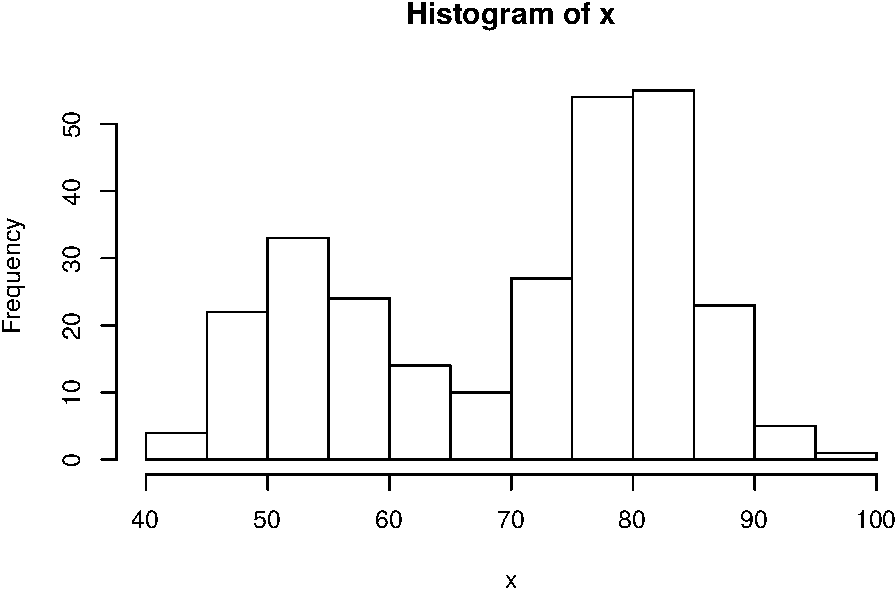
\includegraphics{ds_files/figure-latex/unnamed-chunk-223-1.pdf}

However, the representation and interpretation of the data can sometimes
change considerably if using different visualization parameters. Indeed,
among others, the \texttt{hist()} function includes an option called
\texttt{breaks} that allows the user to specify a vector giving the
number of breakpoints between histogram cells. An example of how this is
used and changes the representation of the data can be found below.

\begin{Shaded}
\begin{Highlighting}[]
\KeywordTok{par}\NormalTok{(}\DataTypeTok{mfrow =} \KeywordTok{c}\NormalTok{(}\DecValTok{1}\NormalTok{,}\DecValTok{2}\NormalTok{))}

\CommentTok{# Histogram with 9 bins}
\NormalTok{bins <-}\StringTok{ }\KeywordTok{seq}\NormalTok{(}\KeywordTok{min}\NormalTok{(x), }\KeywordTok{max}\NormalTok{(x), }\DataTypeTok{length.out =} \DecValTok{10}\NormalTok{)}
\KeywordTok{hist}\NormalTok{(x, }\DataTypeTok{breaks =}\NormalTok{ bins)}

\CommentTok{# Histogram with 19 bins}
\NormalTok{bins <-}\StringTok{ }\KeywordTok{seq}\NormalTok{(}\KeywordTok{min}\NormalTok{(x), }\KeywordTok{max}\NormalTok{(x), }\DataTypeTok{length.out =} \DecValTok{20}\NormalTok{)}
\KeywordTok{hist}\NormalTok{(x, }\DataTypeTok{breaks =}\NormalTok{ bins)}
\end{Highlighting}
\end{Shaded}

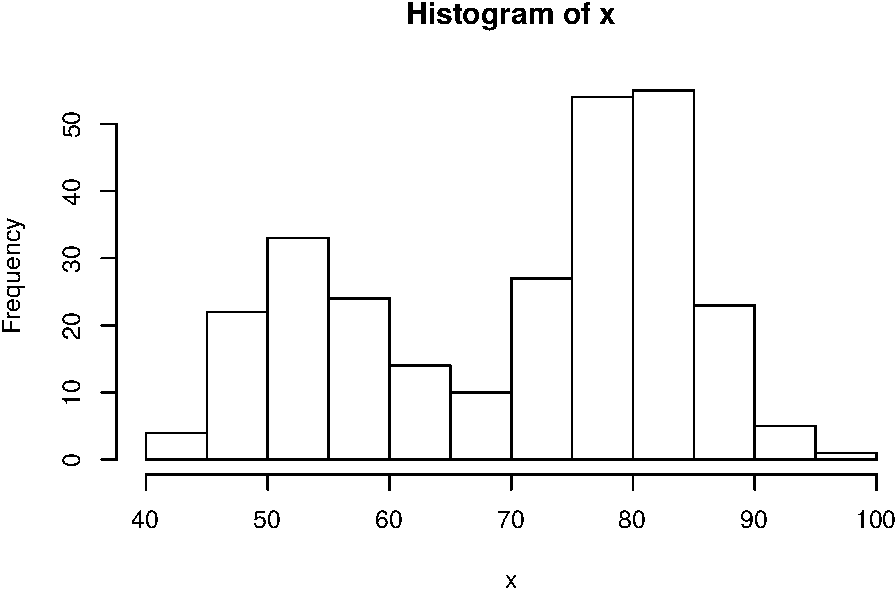
\includegraphics{ds_files/figure-latex/unnamed-chunk-224-1.pdf}

As you may notice, the number of bins created by using this option is
always one unit less than the length of the specified vector (i.e.~9 and
19). Therefore, if we intend to deliver an app that allows the user to
directly specify the number of bins, we should take this into account
and add one unit to the input that the user has given within the
\texttt{length.out} option. Ideally, we would be looking to implement a
function which includes the following steps:

\begin{Shaded}
\begin{Highlighting}[]
\NormalTok{input <-}\StringTok{ }\DecValTok{10}

\CommentTok{# Histogram with input bins}
\NormalTok{bins <-}\StringTok{ }\KeywordTok{seq}\NormalTok{(}\KeywordTok{min}\NormalTok{(x), }\KeywordTok{max}\NormalTok{(x), }\DataTypeTok{length.out =}\NormalTok{ input }\OperatorTok{+}\StringTok{ }\DecValTok{1}\NormalTok{)}
\KeywordTok{hist}\NormalTok{(x, }\DataTypeTok{breaks =}\NormalTok{ bins)}
\end{Highlighting}
\end{Shaded}

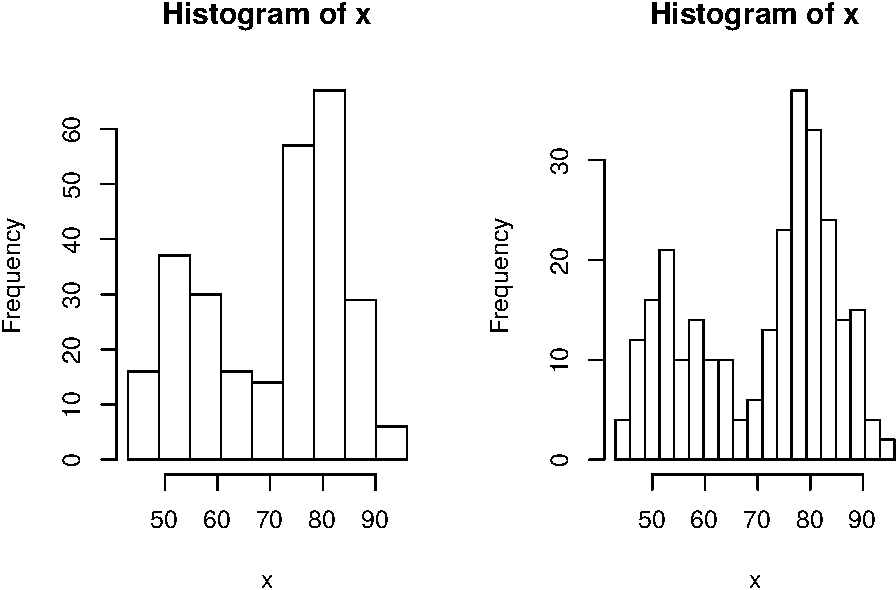
\includegraphics{ds_files/figure-latex/unnamed-chunk-225-1.pdf}

where the value given to the \texttt{input} object (which is 10 in the
above example) is the only value required and can be assigned by the
user through the app interface. The next step will explain how to do so.

\section{Step 2: User Interface (UI) /
Frontend}\label{step-2-user-interface-ui-frontend}

Once we have determined the structure of the code we can now start
creating the Shiny app by firstly developing the UI (or frontend) with
which the user will interact. To address this part, let us take the
tutorial example as a guide and inspect the part of the code related to
the UI.

\begin{Shaded}
\begin{Highlighting}[]
\CommentTok{# Define UI for application that draws a histogram}
\NormalTok{ui <-}\StringTok{ }\KeywordTok{fluidPage}\NormalTok{(}
   
   \CommentTok{# Application title}
   \KeywordTok{titlePanel}\NormalTok{(}\StringTok{"Old Faithful Geyser Data"}\NormalTok{),}
   
   \CommentTok{# Sidebar with a slider input for number of bins }
   \KeywordTok{sidebarLayout}\NormalTok{(}
      \KeywordTok{sidebarPanel}\NormalTok{(}
         \KeywordTok{sliderInput}\NormalTok{(}\StringTok{"bins"}\NormalTok{,}
                     \StringTok{"Number of bins:"}\NormalTok{,}
                     \DataTypeTok{min =} \DecValTok{1}\NormalTok{,}
                     \DataTypeTok{max =} \DecValTok{50}\NormalTok{,}
                     \DataTypeTok{value =} \DecValTok{30}\NormalTok{)}
\NormalTok{      ),}
      
      \CommentTok{# Show a plot of the generated distribution}
      \KeywordTok{mainPanel}\NormalTok{(}
         \KeywordTok{plotOutput}\NormalTok{(}\StringTok{"distPlot"}\NormalTok{)}
\NormalTok{      )}
\NormalTok{   )}
\NormalTok{)}
\end{Highlighting}
\end{Shaded}

As can be seen, all the code that will be dedicated to creating the UI
is assigned to an object called \texttt{ui} through a function called
\texttt{fluidPage()} (see \texttt{?fluidPage} for more information). The
two main elements of this function are the panel dedicated to the title
that will appear for the app (\texttt{titlePanel()}) and the layout to
give to web page which in this example is a layout with a sidebar for
the user to enter their inputs and a main panel in which the outputs
will be visualized (\texttt{sidebarLayout()}). In the next paragraphs we
will provide more details on the possible contents to be presented in
the app interface, as well as the options that can be employed to allow
the user to enter the needed inputs and the options for visualizing the
outputs.

\subsection*{Content Creation}\label{content-creation}


We want to design the application in the way that it is comprehensive
and also easy to interpret. Below are some often-used options of content
creation that will be beneficial to know.

\begin{longtable}[]{@{}ll@{}}
\toprule
Function & Description\tabularnewline
\midrule
\endhead
titlePanel() & The title of the application\tabularnewline
sidebarLayout() & Creates a sidebar layout for
fluidPage()\tabularnewline
sidebarPanel() & Makes a sidebar menu\tabularnewline
mainPanel() & Main content area for different outputs\tabularnewline
\bottomrule
\end{longtable}

\subsection*{Input Controls}\label{input-controls}


We also want to provide spaces so that the client can change any desired
parameter. For example, in the above example, this would be the number
of bins. Below are some input controls the developer can use.

\begin{longtable}[]{@{}ll@{}}
\toprule
Function & Description\tabularnewline
\midrule
\endhead
numericInput() & Number entry input\tabularnewline
radioButtons() & Radio button selection\tabularnewline
selectInput() & Dropdown menu\tabularnewline
sliderInput() & Range slider (1/2 values)\tabularnewline
submitButton() & Submission button\tabularnewline
textInput() & Text input box\tabularnewline
checkboxInput() & Single checkbox input\tabularnewline
dateInput() & Date Selection input\tabularnewline
fileInput() & Upload a file to Shiny\tabularnewline
helpText() & Describe input field\tabularnewline
\bottomrule
\end{longtable}

\subsection*{Output Render Controls}\label{output-render-controls}


The different type of output that is shown can be designed depending on
what the developer intends it to be. Examples of these options are shown
below. We advise you to follow the videos and research different options
that fit the desired output.

\begin{longtable}[]{@{}ll@{}}
\toprule
Function & Description\tabularnewline
\midrule
\endhead
plotOutput() & Display a rendered plot\tabularnewline
tableOutput() & Display in Table\tabularnewline
textOutput() & Formatted Text Output\tabularnewline
uiOutput() & Dynamic UI Elements\tabularnewline
verbatimTextOutput() & ``as is''" Text Output``\tabularnewline
imageOutput() & Render an Image\tabularnewline
htmlOutput() & Render Pure HTML\tabularnewline
\bottomrule
\end{longtable}

\section{Step 3: Implementing the backend
(server)}\label{step-3-implementing-the-backend-server}

This step consists in adapting the structure of the code seen in Step 1
to the requirements of the Shiny app structure. This is done by creating
a function which, as arguments, has an \texttt{input} and an
\texttt{output} as can be seen below always using the example given in
the tutorial.

\begin{Shaded}
\begin{Highlighting}[]
\NormalTok{server <-}\StringTok{ }\ControlFlowTok{function}\NormalTok{(input, output) \{}
   
\NormalTok{   output}\OperatorTok{$}\NormalTok{distPlot <-}\StringTok{ }\KeywordTok{renderPlot}\NormalTok{(\{}
      \CommentTok{# generate bins based on input$bins from ui.R}
\NormalTok{      x    <-}\StringTok{ }\NormalTok{faithful[, }\DecValTok{2}\NormalTok{] }
\NormalTok{      bins <-}\StringTok{ }\KeywordTok{seq}\NormalTok{(}\KeywordTok{min}\NormalTok{(x), }\KeywordTok{max}\NormalTok{(x), }\DataTypeTok{length.out =}\NormalTok{ input}\OperatorTok{$}\NormalTok{bins }\OperatorTok{+}\StringTok{ }\DecValTok{1}\NormalTok{)}
      
      \CommentTok{# draw the histogram with the specified number of bins}
      \KeywordTok{hist}\NormalTok{(x, }\DataTypeTok{breaks =}\NormalTok{ bins, }\DataTypeTok{col =} \StringTok{'darkgray'}\NormalTok{, }\DataTypeTok{border =} \StringTok{'white'}\NormalTok{)}
\NormalTok{   \})}
\NormalTok{\}}
\end{Highlighting}
\end{Shaded}

In this example, the function is called \texttt{server()} and contains
only one object called \texttt{output} with a corresponding element
called \texttt{distPlot} (\texttt{output\$distPlot}). It must be
underlined that the latter name must correspond to the name given for
the output in the UI setup (i.e.~the \texttt{distPlot} name inserted in
\texttt{plotOutput("distPlot")}, see Step 2). The content of the output
in this example is a plot and we therefore use the \texttt{renderPlot()}
function in which we can include the code that we developed in Step 1
(with some added graphical parameters for the color of the bins and
their borders). Of course, this output will depend on the input provided
by the user which is used when defining the \texttt{bins} object (i.e.
\texttt{bins\ \textless{}-\ seq(min(x),\ max(x),\ length.out\ =\ input\$bins\ +\ 1)}).
Just like for the \texttt{output} object, also in this case the
\texttt{input} object has an element whose name must correspond to the
name given for the input when building the UI (i.e.
\texttt{sliderInput("bins",...)}).

\section{Step 4: Connecting frontend and
backend}\label{step-4-connecting-frontend-and-backend}

Once we have developed the structure and defined the functions and
objects for the UI (frontend) and backend environments, all that needs
to be done is to ensure that they can communicate with each other. Using
the Shiny environment, this can be quickly and easily done by using the
\texttt{shinyApp()} function which takes the object defining the UI
interface (\texttt{ui} in our example, see Step 2) and the function that
takes the input and delivers the output (\texttt{server} in our example,
see Step 3).

\begin{Shaded}
\begin{Highlighting}[]
\KeywordTok{shinyApp}\NormalTok{(}\DataTypeTok{ui =}\NormalTok{ ui, }\DataTypeTok{server =}\NormalTok{ server)}
\end{Highlighting}
\end{Shaded}

Therefore, having completed the UI and backend code, to launch the Shiny
Web app you simply need to execute this code (or push the ``Run App''
button at the top of your Shiny app code).

\section{Step 5: Customize}\label{step-5-customize}

We can confidently say that shiny can be heavily customized, like how
webpage applications are customized, even without explicitly using
complex javascript or HTML elements.

One of such examples are a \texttt{submitButton(...)}, in which we can
run responsive output from input data using a button to initiate. More
can be read from
\href{https://shiny.rstudio.com/reference/shiny/1.0.4/submitButton.html}{here}.

Another of such example is controlling the content creation process
other than the default.

\section{Example: Monte-Carlo
Integration}\label{example-monte-carlo-integration-1}

\section{Example: Buffon's needle}\label{example-buffons-needle}

In 1777, the French nobleman Georges-Louis Leclerc, Compte de Buffon
(Count of Buffon) posed the following problem to the Royal Academy of
Sciences in Paris \citep{buffon1777essai}:

\begin{quote}
Suppose that you drop a needle of unit length on a plane ruled by the
lines \(y = m \; (m = 0, \pm 1, \pm 2, ...)\) - what is then the
probability that the needle comes to lie in a position where it crosses
one of the lines?
\end{quote}

Compte de Buffon also provided the answer and showed that the needle
will intersect lines with a predictable probability. In mathematical
terms, his solution (still known today as the Buffon principle) can be
stated as follows:

\begin{equation} 
\mathbb{P}(\text{intersection}) = \frac{2}{\pi}.
\label{eq:probbuffon}
\end{equation}

If you are curious about the derivation of this result, click on the
button below.

Derivation - Equation (7.1)

\hypertarget{hideclass2}{}
\BeginKnitrBlock{rmdtip}
This proof is based on the solution of Example 4.5.8 of
\citet{grimmett2001probability}. We start by letting \((X, Y)\) denote
the coordinates of the point at the center of the needle and let
\(\Theta\) be the angle, modulo \(\pi\), that lies between the needle
and the horizontal lines. Next, we define the distance from the needle's
center to the nearest line beneath it as \(Z = Y - \lfloor Y \rfloor\),
where \(\lfloor Y \rfloor\) denotes the ``floor'' of \(Y\), i.e.~the
greatest integer not greater than \(Y\). Since the needle is randomly
casted, we have that the joint density of \((Z, \Theta)\) is given by:

\[
f_{Z, \Theta} (z, \theta) = f_{Z} (z) f_{\Theta} (\theta) = \frac{1}{\pi},
\]

for \(0 \leq z \leq 1\) and \(0 \leq \theta \leq \pi\). By drawing a
diagram one can see that an interception occurs if and only if
\((Z, \Theta) \in \mathcal{B}\), where

\[
\mathcal{B} = \left\{(z, \theta)\,: \;\; z \leq \frac{1}{2} \sin (\theta)  \;\; \text{or} \;\; 1-z \leq \frac{1}{2} \sin(\theta)\right\}.
\]

Therefore, we obtain

\[
\mathbb{P}(\text{intersection}) = \iint_\mathcal{B} \; f_{Z, \Theta} (z, \theta)\, dz \, d\theta = \frac{1}{\pi} \int_0^\pi \left(\int_0^{\frac{1}{2}\sin(\theta)} dz + \int_{1 - \frac{1}{2}\sin(\theta)}^{1} dz \right) d\theta = \frac{2}{\pi},
\]

which verifies Equation \eqref{eq:probbuffon} and concludes the proof.
\EndKnitrBlock{rmdtip}

\newline

Georges-Louis Leclerc's motivation behind this problem was to design an
experiment to estimate the value of \(\pi\). Indeed, if you fling a
needle a large number \(B\) times onto a ruled plane and count the
number of times \(S_B\) that the needle intersects a line, we might be
able to approximate \(\mathbb{P}(\text{intersection})\) and therefore
\(\pi\). From Equation \eqref{eq:probbuffon}, we know that the proportion
\(S_B/B\) will be ``close'' to the probability
\(\mathbb{P}(\text{intersection})\). In fact the (weak) law of large
number garantees that \(S_B/B\) converges (in probability) to \(2/\pi\),
i.e.~for any given \(\varepsilon > 0\),

\[
\lim_{B \rightarrow \infty} \; \mathbb{P}\left( \left| \frac{S_B}{B} - \frac{2}{\pi} \right|  > \varepsilon \right) = 0.
\]

Thus, the estimator

\[
\hat{\pi}_B = \frac{2B}{S_B},
\]

is a plausible estimator of \(\pi\). The Continous Mapping Theorem
\citep[see e.g.~Theorem 1.14 of][]{dasgupta2008asymptotic} can (among
others) be used to show that \(\hat{\pi}\) is a \textbf{consistent}
estimator of \(\pi\) (i.e. \(\hat{\pi}\) converges in probability to
\(\pi\)). In 1777, Georges-Louis Leclerc investigated this problem and
computed \(\hat{\pi}_B\) by flinging a needle 2084 times, which may
consitute the first recorded example of a Monte-Carlo method
(simulation?) in use.

To illustrate the convergence of our estimator we could fling a needle
\(B\) times and compute the following estimators:

\[
\hat{\pi}_j = \frac{2j}{S_j}, \;\; j = k,\, ...., \,B
\]

where \(k \ll B\). Once this is done, we could create a graph with \(j\)
on the horizontal axis and \(\hat{\pi}_j\) on the vertical axis. Since
\(\hat{\pi}_B\) is a consistent estimator we should see that
\(\hat{\pi}_j\) tends to get closer and closer to \(\pi\) as \(j\)
increases. In this graph we could also superimpose several experiments
(recasting the needle \(B\) times several times) to reinforce our
argument.

The goal of this example is to create a Shiny app to visualize and
illustrate Buffon's needle experiment. For this purpose, we will use the
following steps:

\begin{enumerate}
\def\labelenumi{\arabic{enumi})}
\tightlist
\item
  \textbf{Step 1: Backend}: Create all the functions needed for the
  backend of our app. A possible approach is to create the following
  functions:

  \begin{enumerate}
  \def\labelenumii{\alph{enumii})}
  \tightlist
  \item
    \texttt{cast\_needle()}: this function randomly casts a needle on
    plane and returns its coordinates as well as a binary variable to
    indicate if the needle crossed a line;
  \item
    \texttt{buffon\_experiment()}: this function performs a Monte-Carlo
    experiment by flinging a large number of needles using the function
    \texttt{cast\_needle()};
  \item
    \texttt{plot.buffon\_experiment()}: to visualize the experiment
    (i.e.~show all the needles randomly dropped) and compute the
    estimator \(\hat{\pi}_B\) for the experiment at hand;
  \end{enumerate}
\end{enumerate}

\begin{enumerate}
\def\labelenumi{\alph{enumi})}
\setcounter{enumi}{3}
\tightlist
\item
  \texttt{converge()}: to illustrate the convergence of the estimator by
  creating the graph mentioned at the end of the previous paragraph.
\end{enumerate}

\begin{enumerate}
\def\labelenumi{\arabic{enumi})}
\setcounter{enumi}{1}
\tightlist
\item
  \textbf{Step 2: Frontend}: Create widgets to collect all inputs needed
  by the backend:

  \begin{enumerate}
  \def\labelenumii{\alph{enumii})}
  \tightlist
  \item
    dimension of the plane on which the needles are dropped;
  \item
    the number of needles being used, i.e. \(B\);
  \item
    number of experiments which is needed to illustrate the convergence
    of the estimator;
  \item
    the seed to allow ``replicable'' experiments. Aside from allowing
    the user to enter these variables, we will need to create two output
    ``tabs''. In the first one, we will ``print'' the result(s) of the
    experiment and in the second one we will illustrate the convergence
    of the estimator. Finally, we will need a button to ``run'' a new
    experiment.
  \end{enumerate}
\item
  \textbf{Step 3: Connecting frontend and backend}: In this third step
  we will need to connect the inputs with the outputs. Indeed, we will
  use the \texttt{input} list created by the widget defined in the
  previous step (Step 2) to create the graphs to be displayed in the two
  output tabs. We will also need to ``activate'' the button
  (i.e.~connect the inputs to the appropriate functions) in order to run
  a new experiment and update the ``seed'' after every new experiment.
\end{enumerate}

To summarize, our approach should follow the steps presented in the
chart below:

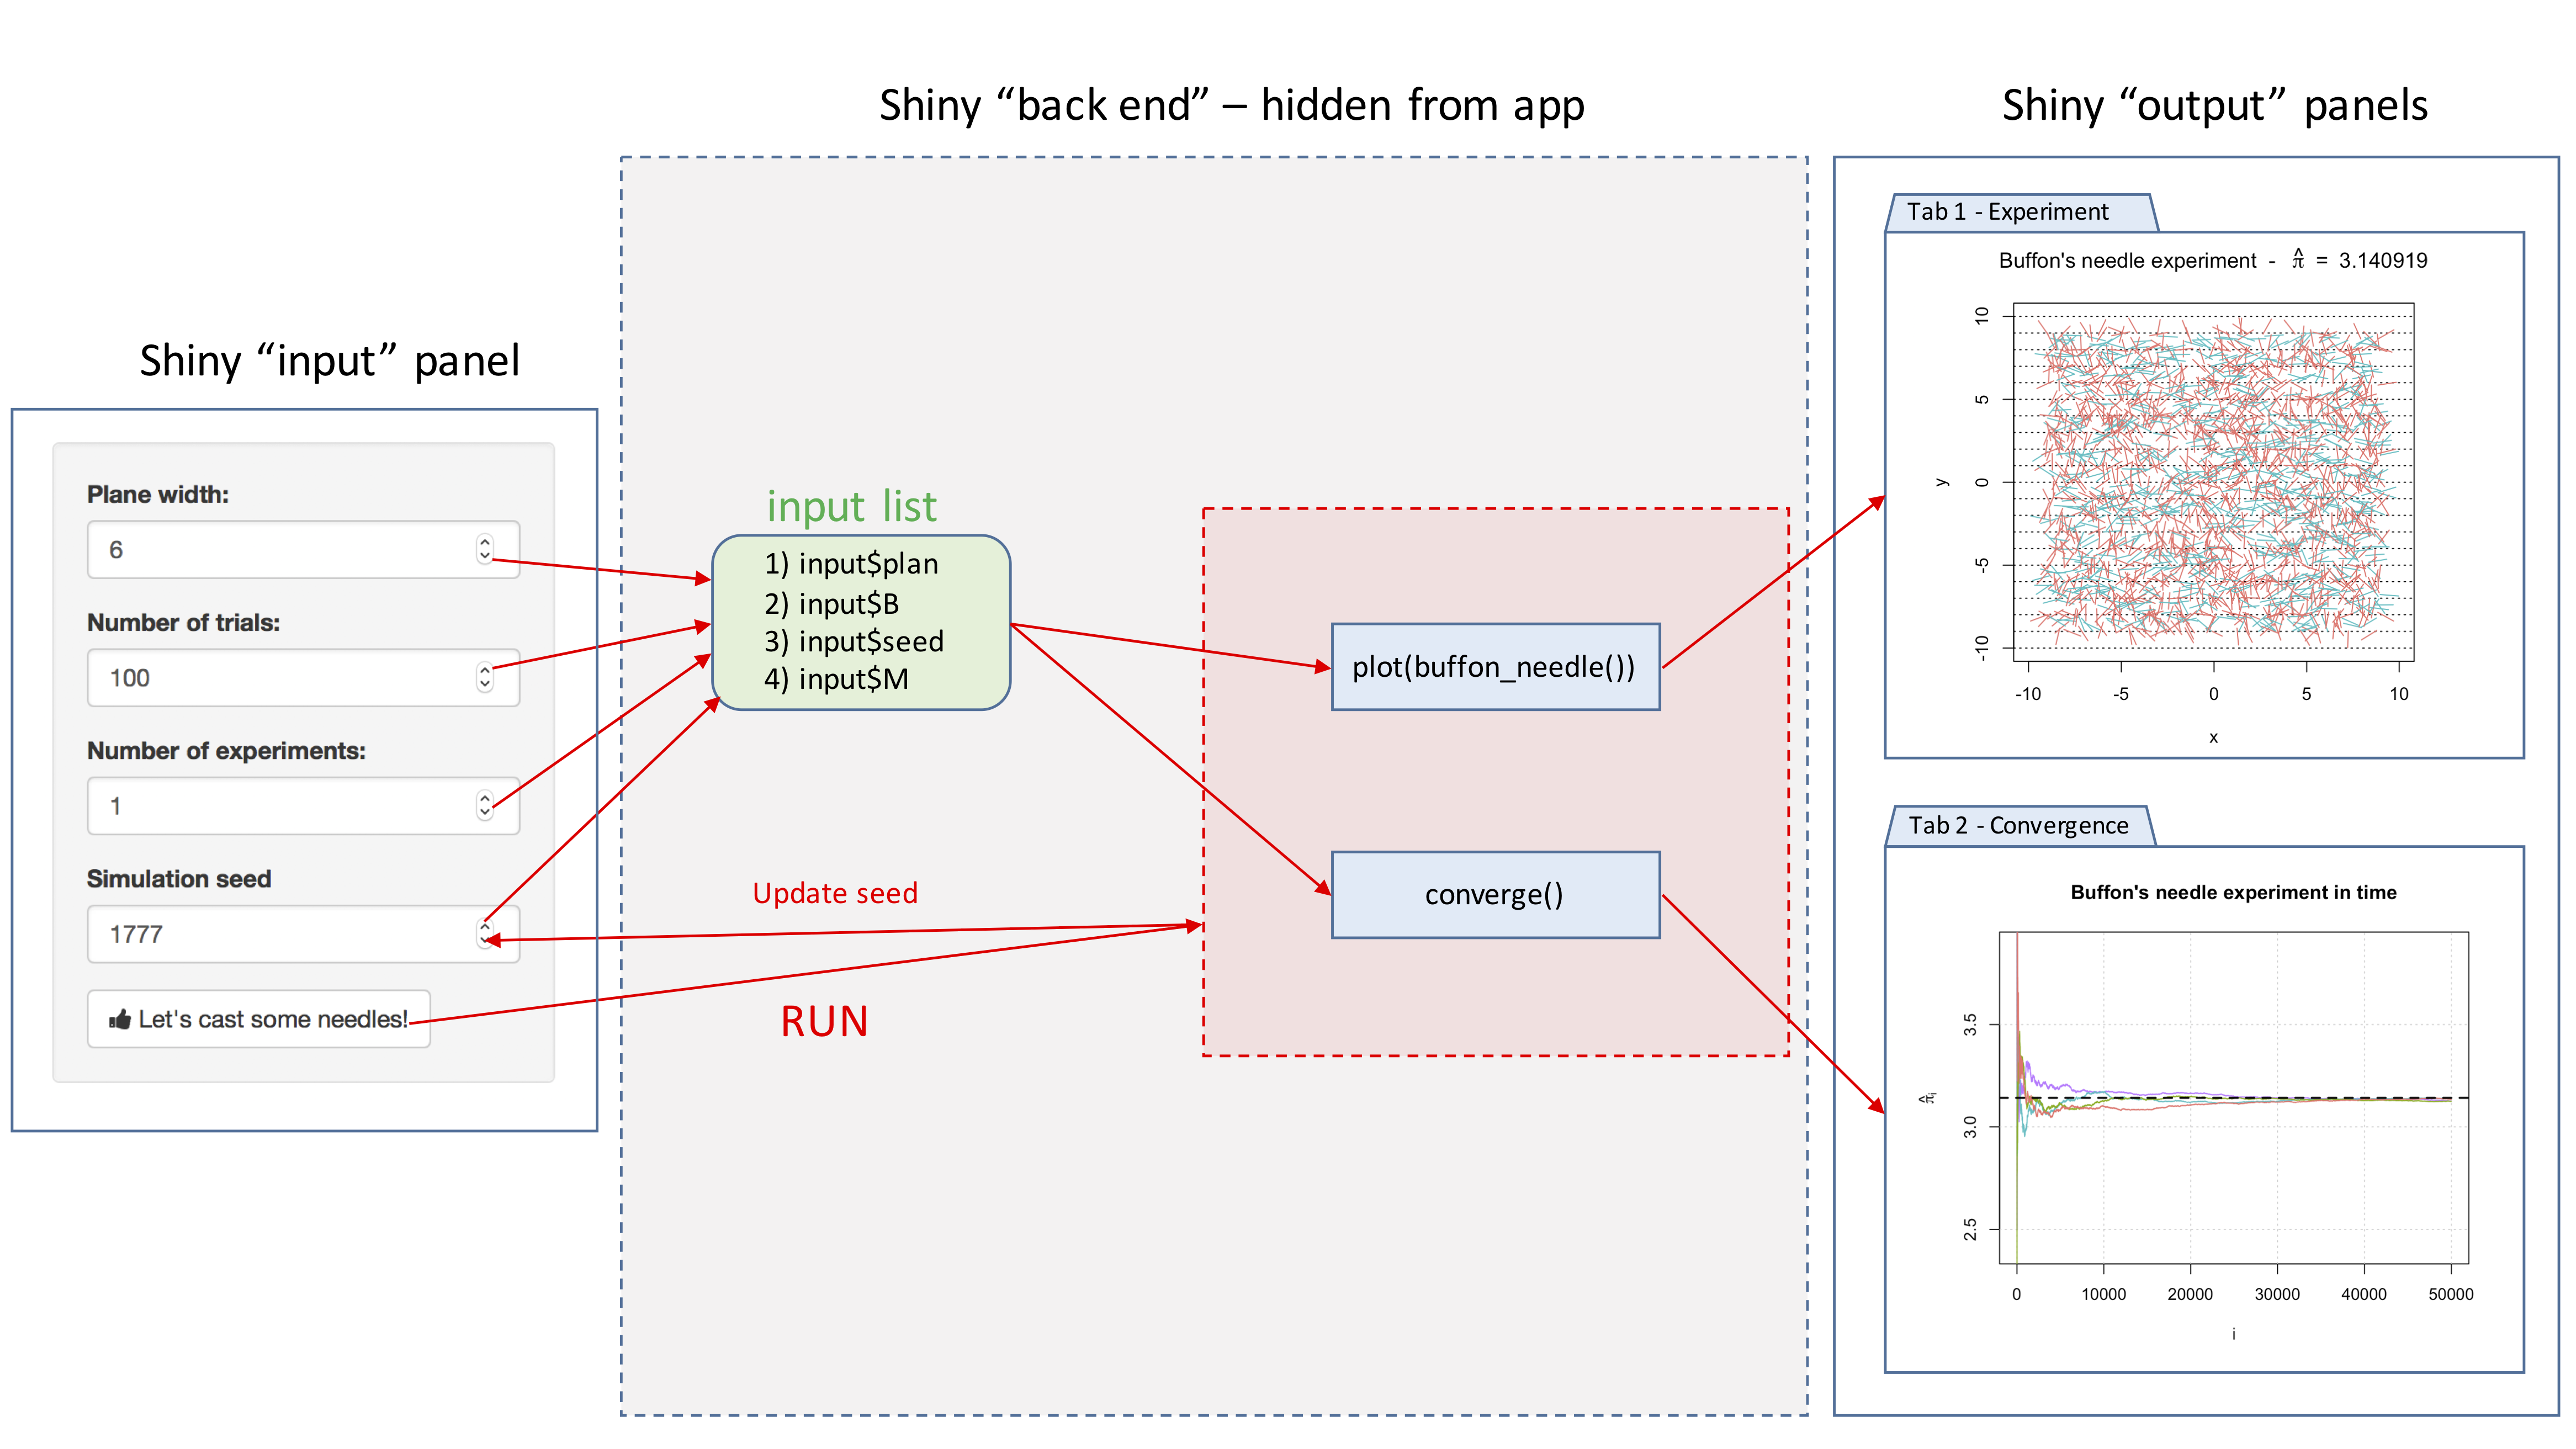
\includegraphics{images/buffon.png}

In the next sections, we will discuss in detail how to program each
step.

\subsection{Step 1: Backend}\label{step-1-backend}

Let us start with the function \texttt{cast\_needle()}. This function
has a single input, i.e.~the width of the (square) plane on which the
needle is cast and returns a \texttt{list} containing:

\begin{itemize}
\tightlist
\item
  \texttt{\$start}: the coordinates of one end of the needle;
\item
  \texttt{\$end}: the coordinates of the other end of the needle;
\item
  \texttt{\$cross}: a binary variable to indicate if the needle
  intercepts a line.
\end{itemize}

\BeginKnitrBlock{rmdnote}
An additional input could be added consisting in the length of the
needle. However, in this example we only consider needles of unit
length.
\EndKnitrBlock{rmdnote}

A possible implementation of this function is given below:

\begin{Shaded}
\begin{Highlighting}[]
\NormalTok{cast_needle <-}\StringTok{ }\ControlFlowTok{function}\NormalTok{(}\DataTypeTok{plane_width =} \DecValTok{20}\NormalTok{)\{}
\NormalTok{  available_range <-}\StringTok{ }\NormalTok{plane_width}\OperatorTok{/}\DecValTok{2} \OperatorTok{-}\StringTok{ }\DecValTok{1} \CommentTok{# where 1 is the length of the needle (unit)}
\NormalTok{  x_start <-}\StringTok{ }\KeywordTok{runif}\NormalTok{(}\DecValTok{2}\NormalTok{, }\OperatorTok{-}\NormalTok{available_range, available_range)}
\NormalTok{  angle <-}\StringTok{ }\KeywordTok{runif}\NormalTok{(}\DecValTok{1}\NormalTok{, }\DecValTok{0}\NormalTok{, }\DecValTok{2}\OperatorTok{*}\NormalTok{pi)}
\NormalTok{  x_end <-}\StringTok{ }\KeywordTok{c}\NormalTok{(}\KeywordTok{cos}\NormalTok{(angle), }\KeywordTok{sin}\NormalTok{(angle)) }\OperatorTok{+}\StringTok{ }\NormalTok{x_start }\CommentTok{# where the angles are multiplied by the needle length which is 1 in this example}
\NormalTok{  cross <-}\StringTok{ }\KeywordTok{floor}\NormalTok{(x_start[}\DecValTok{2}\NormalTok{]) }\OperatorTok{!=}\StringTok{ }\KeywordTok{floor}\NormalTok{(x_end[}\DecValTok{2}\NormalTok{])}
\NormalTok{  out <-}\StringTok{ }\KeywordTok{list}\NormalTok{(}\DataTypeTok{start =}\NormalTok{ x_start, }\DataTypeTok{end =}\NormalTok{ x_end, }\DataTypeTok{cross =}\NormalTok{ cross)}
\NormalTok{  out}
\NormalTok{\}}
\end{Highlighting}
\end{Shaded}

Here is an example of the output of this function:

\begin{Shaded}
\begin{Highlighting}[]
\NormalTok{needle <-}\StringTok{ }\KeywordTok{cast_needle}\NormalTok{(}\DataTypeTok{plane_width =} \DecValTok{4}\NormalTok{)}
\NormalTok{needle}
\end{Highlighting}
\end{Shaded}

\begin{verbatim}
## $start
## [1] 0.1307334 0.3302562
## 
## $end
## [1] 0.1470854 1.3301225
## 
## $cross
## [1] TRUE
\end{verbatim}

and we could now for example provide the following graphical
representation of this random cast:

\begin{Shaded}
\begin{Highlighting}[]
\KeywordTok{plot}\NormalTok{(}\OtherTok{NA}\NormalTok{, }\DataTypeTok{xlim =} \KeywordTok{c}\NormalTok{(}\OperatorTok{-}\DecValTok{2}\NormalTok{, }\DecValTok{2}\NormalTok{), }\DataTypeTok{ylim =} \KeywordTok{c}\NormalTok{(}\OperatorTok{-}\DecValTok{2}\NormalTok{, }\DecValTok{2}\NormalTok{), }\DataTypeTok{xlab =} \StringTok{"x"}\NormalTok{, }\DataTypeTok{ylab =} \StringTok{"y"}\NormalTok{)}
\KeywordTok{abline}\NormalTok{(}\DataTypeTok{h =} \OperatorTok{-}\DecValTok{2}\OperatorTok{:}\DecValTok{2}\NormalTok{, }\DataTypeTok{lty =} \DecValTok{3}\NormalTok{)}
\KeywordTok{lines}\NormalTok{(}\KeywordTok{c}\NormalTok{(needle}\OperatorTok{$}\NormalTok{start[}\DecValTok{1}\NormalTok{], needle}\OperatorTok{$}\NormalTok{end[}\DecValTok{1}\NormalTok{]), }\KeywordTok{c}\NormalTok{(needle}\OperatorTok{$}\NormalTok{start[}\DecValTok{2}\NormalTok{], needle}\OperatorTok{$}\NormalTok{end[}\DecValTok{2}\NormalTok{]))}
\end{Highlighting}
\end{Shaded}

\begin{center}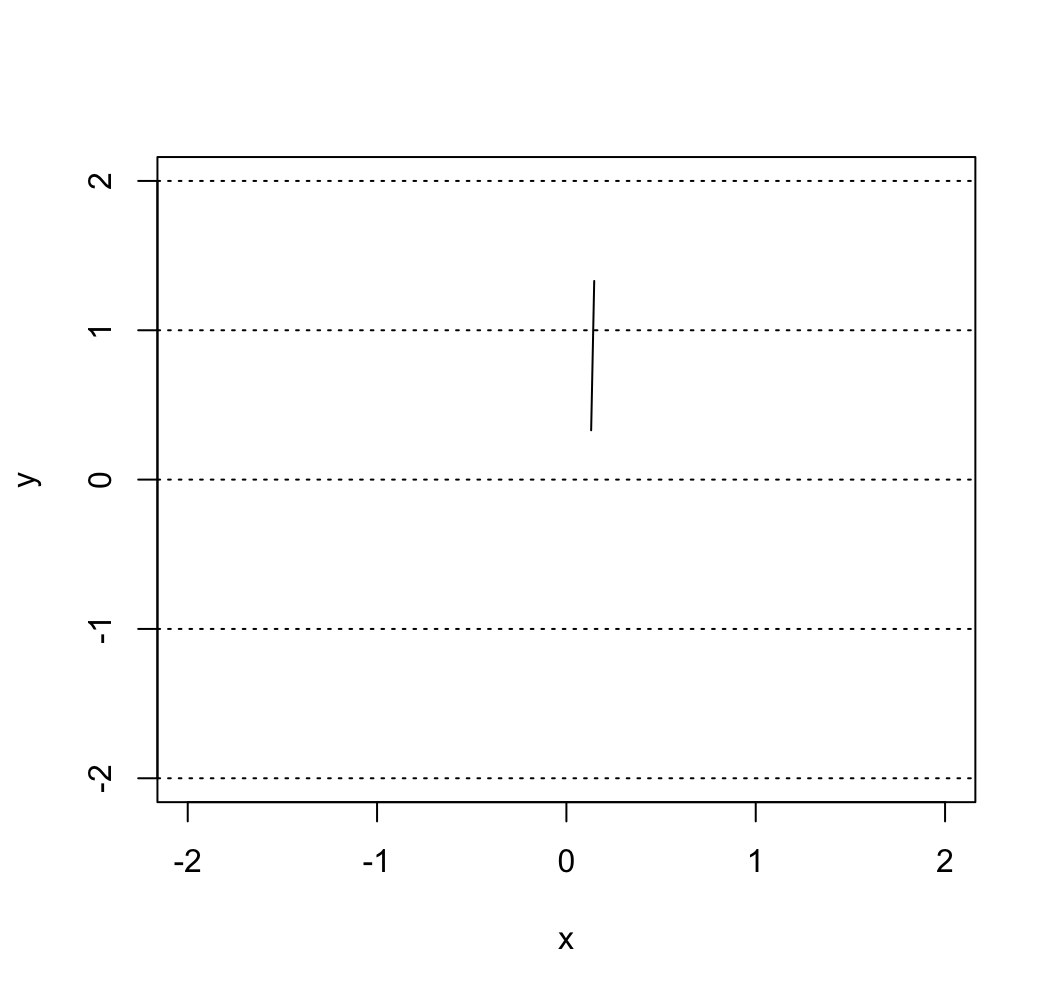
\includegraphics{ds_files/figure-latex/unnamed-chunk-234-1} \end{center}

Next, we consider the function \texttt{buffon\_experiment()}. This
function is based on the previous function and contains the following
inputs:

\begin{itemize}
\tightlist
\item
  \texttt{B}: the number of needles being casted;
\item
  \texttt{plane\_width}: the width of the (square) plane on which the
  needles are casted;
\item
  \texttt{seed}: the ``seed'' used by the random number generator
  (allows to replicate results);
\end{itemize}

and returns a \texttt{list} containing:

\begin{itemize}
\tightlist
\item
  \texttt{\$start}: a \(B \times 2\) matrix containing the coordinates
  of one end of the \(B\) needles;
\item
  \texttt{\$end}: a \(B \times 2\) matrix containing the coordinates of
  the other end of the \(B\) needles;
\item
  \texttt{\$cross}: a vector of length \(B\) containing boolean
  variables to indicate whether a needle crosses a line or not;
\item
  \texttt{\$plane}: the width of the (square) plane.
\end{itemize}

A possible implementation of this function is provided below:

\begin{Shaded}
\begin{Highlighting}[]
\NormalTok{buffon_experiment <-}\StringTok{ }\ControlFlowTok{function}\NormalTok{(}\DataTypeTok{B =} \DecValTok{2084}\NormalTok{, }\DataTypeTok{plane_width =} \DecValTok{10}\NormalTok{, }\DataTypeTok{seed =} \OtherTok{NULL}\NormalTok{)\{}
  
  \ControlFlowTok{if}\NormalTok{ (}\OperatorTok{!}\KeywordTok{is.null}\NormalTok{(seed))\{}
    \KeywordTok{set.seed}\NormalTok{(seed)}
\NormalTok{  \}}
  
\NormalTok{  X_start <-}\StringTok{ }\NormalTok{X_end <-}\StringTok{ }\KeywordTok{matrix}\NormalTok{(}\OtherTok{NA}\NormalTok{, B, }\DecValTok{2}\NormalTok{) }
\NormalTok{  cross <-}\StringTok{ }\KeywordTok{rep}\NormalTok{(}\OtherTok{NA}\NormalTok{, B)}
  
  \ControlFlowTok{for}\NormalTok{ (i }\ControlFlowTok{in} \DecValTok{1}\OperatorTok{:}\NormalTok{B)\{}
\NormalTok{    inter <-}\StringTok{ }\KeywordTok{cast_needle}\NormalTok{(}\DataTypeTok{plane_width =}\NormalTok{ plane_width)}
\NormalTok{    X_start[i, ] <-}\StringTok{ }\NormalTok{inter}\OperatorTok{$}\NormalTok{start}
\NormalTok{    X_end[i, ] <-}\StringTok{ }\NormalTok{inter}\OperatorTok{$}\NormalTok{end}
\NormalTok{    cross[i] <-}\StringTok{ }\NormalTok{inter}\OperatorTok{$}\NormalTok{cross}
\NormalTok{  \}}
  
\NormalTok{  out <-}\StringTok{ }\KeywordTok{list}\NormalTok{(}\DataTypeTok{start =}\NormalTok{ X_start, }\DataTypeTok{end =}\NormalTok{ X_end, }\DataTypeTok{cross =}\NormalTok{ cross, }\DataTypeTok{plane =}\NormalTok{ plane_width)}
  \KeywordTok{class}\NormalTok{(out) <-}\StringTok{ "buffon_experiment"}
\NormalTok{  out}
\NormalTok{\}}
\end{Highlighting}
\end{Shaded}

For example, if we consider an experiment where four needles are cast,
we could obtain:

\begin{Shaded}
\begin{Highlighting}[]
\NormalTok{experiment <-}\StringTok{ }\KeywordTok{buffon_experiment}\NormalTok{(}\DataTypeTok{B =} \DecValTok{4}\NormalTok{, }\DataTypeTok{plane_width =} \DecValTok{4}\NormalTok{)}
\NormalTok{experiment}
\end{Highlighting}
\end{Shaded}

\begin{verbatim}
## $start
##            [,1]         [,2]
## [1,]  0.5668833 -0.719905025
## [2,]  0.7966649  0.304674088
## [3,] -0.7692311 -0.007315481
## [4,]  0.2704636 -0.262152664
## 
## $end
##             [,1]       [,2]
## [1,] -0.24968864 -0.1426613
## [2,] -0.17226155  0.5520232
## [3,] -0.05723734 -0.7095013
## [4,]  0.16782619  0.7325662
## 
## $cross
## [1] FALSE FALSE FALSE  TRUE
## 
## $plane
## [1] 4
## 
## attr(,"class")
## [1] "buffon_experiment"
\end{verbatim}

which could be represented as

\begin{Shaded}
\begin{Highlighting}[]
\KeywordTok{plot}\NormalTok{(}\OtherTok{NA}\NormalTok{, }\DataTypeTok{xlim =} \KeywordTok{c}\NormalTok{(}\OperatorTok{-}\DecValTok{2}\NormalTok{, }\DecValTok{2}\NormalTok{), }\DataTypeTok{ylim =} \KeywordTok{c}\NormalTok{(}\OperatorTok{-}\DecValTok{2}\NormalTok{, }\DecValTok{2}\NormalTok{), }\DataTypeTok{xlab =} \StringTok{"x"}\NormalTok{, }\DataTypeTok{ylab =} \StringTok{"y"}\NormalTok{)}
\KeywordTok{abline}\NormalTok{(}\DataTypeTok{h =} \OperatorTok{-}\DecValTok{2}\OperatorTok{:}\DecValTok{2}\NormalTok{, }\DataTypeTok{lty =} \DecValTok{3}\NormalTok{)}
\ControlFlowTok{for}\NormalTok{ (i }\ControlFlowTok{in} \DecValTok{1}\OperatorTok{:}\DecValTok{4}\NormalTok{)\{}
  \KeywordTok{lines}\NormalTok{(}\KeywordTok{c}\NormalTok{(experiment}\OperatorTok{$}\NormalTok{start[i,}\DecValTok{1}\NormalTok{], experiment}\OperatorTok{$}\NormalTok{end[i,}\DecValTok{1}\NormalTok{]), }
        \KeywordTok{c}\NormalTok{(experiment}\OperatorTok{$}\NormalTok{start[i,}\DecValTok{2}\NormalTok{], experiment}\OperatorTok{$}\NormalTok{end[i,}\DecValTok{2}\NormalTok{]))}
\NormalTok{\}}
\end{Highlighting}
\end{Shaded}

\begin{center}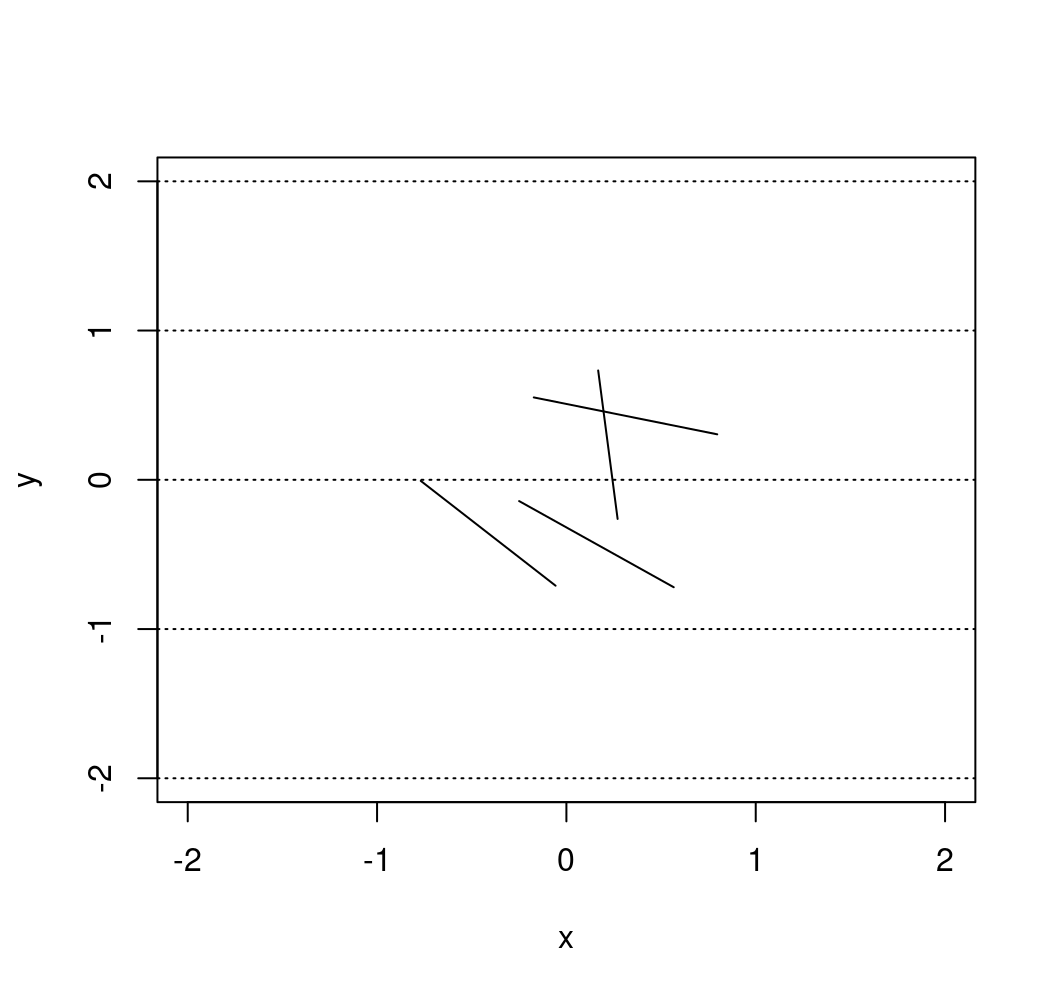
\includegraphics{ds_files/figure-latex/unnamed-chunk-237-1} \end{center}

We can now write a custom \texttt{plot()} function for the output of the
function \texttt{buffon\_experiment()}. This function will provide a way
to visualize the experiment and will compute \(\hat{\pi}_B\), which will
be shown in the title. A possible function is provided below:

\begin{Shaded}
\begin{Highlighting}[]
\NormalTok{plot.buffon_experiment <-}\StringTok{ }\ControlFlowTok{function}\NormalTok{(obj)\{}
\NormalTok{  cross <-}\StringTok{ }\NormalTok{obj}\OperatorTok{$}\NormalTok{cross}
\NormalTok{  X_start <-}\StringTok{ }\NormalTok{obj}\OperatorTok{$}\NormalTok{start}
\NormalTok{  X_end <-}\StringTok{ }\NormalTok{obj}\OperatorTok{$}\NormalTok{end}
\NormalTok{  B <-}\StringTok{ }\KeywordTok{length}\NormalTok{(cross)}
\NormalTok{  cols <-}\StringTok{ }\KeywordTok{rev}\NormalTok{(}\KeywordTok{hcl}\NormalTok{(}\DataTypeTok{h =} \KeywordTok{seq}\NormalTok{(}\DecValTok{15}\NormalTok{, }\DecValTok{375}\NormalTok{, }\DataTypeTok{length =} \DecValTok{3}\NormalTok{), }\DataTypeTok{l =} \DecValTok{65}\NormalTok{, }\DataTypeTok{c =} \DecValTok{100}\NormalTok{)[}\DecValTok{1}\OperatorTok{:}\DecValTok{2}\NormalTok{])}
  
\NormalTok{  title_part1 <-}\StringTok{ 'Buffon}\CharTok{\textbackslash{}'}\StringTok{s needle experiment  -  '}
\NormalTok{  title_part2 <-}\StringTok{ ' = '}
\NormalTok{  pi_hat <-}\StringTok{ }\KeywordTok{round}\NormalTok{(}\DecValTok{2}\OperatorTok{/}\KeywordTok{mean}\NormalTok{(obj}\OperatorTok{$}\NormalTok{cross), }\DecValTok{6}\NormalTok{)}
  
\NormalTok{  title <-}\StringTok{ }\KeywordTok{bquote}\NormalTok{(.(title_part1) }\OperatorTok{~}\StringTok{ }\KeywordTok{hat}\NormalTok{(pi)[B] }\OperatorTok{~}\StringTok{ }\NormalTok{.(title_part2) }\OperatorTok{~}\StringTok{ }\NormalTok{.(pi_hat))}
  
  \KeywordTok{plot}\NormalTok{(}\OtherTok{NA}\NormalTok{, }\DataTypeTok{xlab =} \StringTok{"x"}\NormalTok{, }\DataTypeTok{ylab =} \StringTok{"y"}\NormalTok{, }\DataTypeTok{xlim =} \KeywordTok{c}\NormalTok{(}\OperatorTok{-}\NormalTok{obj}\OperatorTok{$}\NormalTok{plane}\OperatorTok{/}\DecValTok{2}\NormalTok{, obj}\OperatorTok{$}\NormalTok{plane}\OperatorTok{/}\DecValTok{2}\NormalTok{), }
       \DataTypeTok{ylim =} \KeywordTok{c}\NormalTok{(}\OperatorTok{-}\NormalTok{obj}\OperatorTok{$}\NormalTok{plan}\OperatorTok{/}\DecValTok{2}\NormalTok{, obj}\OperatorTok{$}\NormalTok{plan}\OperatorTok{/}\DecValTok{2}\NormalTok{), }
       \DataTypeTok{main =}\NormalTok{ title)}
  \KeywordTok{abline}\NormalTok{(}\DataTypeTok{h =}\NormalTok{ (}\OperatorTok{-}\NormalTok{obj}\OperatorTok{$}\NormalTok{plan)}\OperatorTok{:}\NormalTok{obj}\OperatorTok{$}\NormalTok{plan, }\DataTypeTok{lty =} \DecValTok{3}\NormalTok{)}
  
  \ControlFlowTok{for}\NormalTok{ (i }\ControlFlowTok{in} \DecValTok{1}\OperatorTok{:}\NormalTok{B)\{}
    \KeywordTok{lines}\NormalTok{(}\KeywordTok{c}\NormalTok{(X_start[i,}\DecValTok{1}\NormalTok{], X_end[i,}\DecValTok{1}\NormalTok{]), }\KeywordTok{c}\NormalTok{(X_start[i,}\DecValTok{2}\NormalTok{], X_end[i,}\DecValTok{2}\NormalTok{]), }
          \DataTypeTok{col =}\NormalTok{ cols[cross[i] }\OperatorTok{+}\StringTok{ }\DecValTok{1}\NormalTok{])}
\NormalTok{  \}}
\NormalTok{\}}
\end{Highlighting}
\end{Shaded}

Therefore, we could now run the same experiment as Georges-Louis Leclerc
by flinging 2084 needles almost instanteously (which is the default
value in the \texttt{buffon\_experiment()} function we created):

\begin{Shaded}
\begin{Highlighting}[]
\NormalTok{experiment <-}\StringTok{ }\KeywordTok{buffon_experiment}\NormalTok{(}\DataTypeTok{B =} \DecValTok{2084}\NormalTok{)}
\KeywordTok{plot}\NormalTok{(experiment)}
\end{Highlighting}
\end{Shaded}

\begin{center}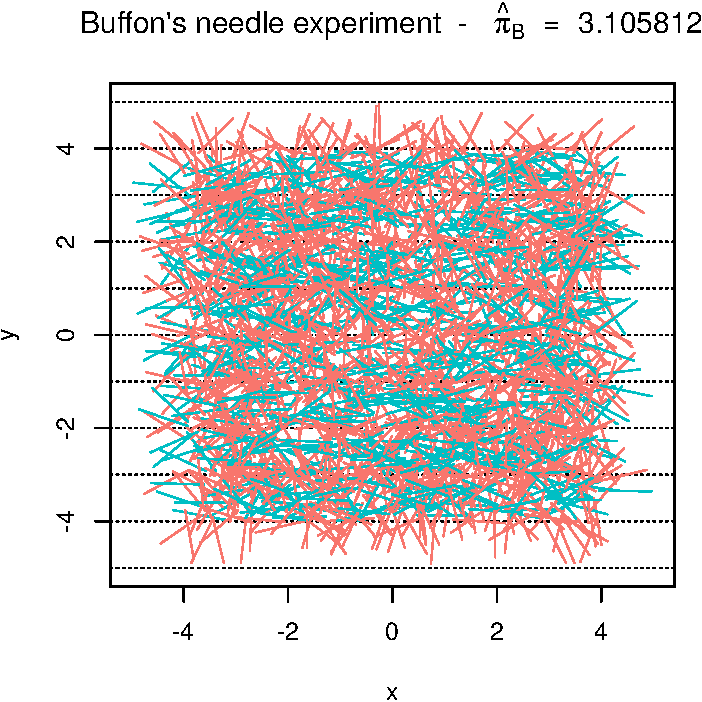
\includegraphics{ds_files/figure-latex/unnamed-chunk-239-1} \end{center}

Finally, we can consider the function \texttt{converge()}. Similarly to
\texttt{buffon\_experiment()}, the function \texttt{converge()} has the
following inputs:

\begin{itemize}
\tightlist
\item
  \texttt{B}: the number of needles being cast;
\item
  \texttt{plane\_width}: the width of the (square) plane on which the
  needles are cast;
\item
  \texttt{seed}: the ``seed'' used by the random number generator
  (allows to replicate results);
\item
  \texttt{M}: the number of experiments.
\end{itemize}

The function returns the graph mentioned at the end of the previous
section. A possible implementation of this function is provided below:

\begin{Shaded}
\begin{Highlighting}[]
\NormalTok{converge <-}\StringTok{ }\ControlFlowTok{function}\NormalTok{(}\DataTypeTok{B =} \DecValTok{2084}\NormalTok{, }\DataTypeTok{plane_width =} \DecValTok{10}\NormalTok{, }\DataTypeTok{seed =} \DecValTok{1777}\NormalTok{, }\DataTypeTok{M =} \DecValTok{12}\NormalTok{)\{}
  
  \ControlFlowTok{if}\NormalTok{ (B }\OperatorTok{<}\StringTok{ }\DecValTok{10}\NormalTok{)\{}
    \KeywordTok{warning}\NormalTok{(}\StringTok{"B was changed to 10"}\NormalTok{)}
\NormalTok{    B <-}\StringTok{ }\DecValTok{10}
\NormalTok{  \}}
  
\NormalTok{  pi_hat <-}\StringTok{ }\KeywordTok{matrix}\NormalTok{(}\OtherTok{NA}\NormalTok{, B, M)}
\NormalTok{  trials <-}\StringTok{ }\DecValTok{1}\OperatorTok{:}\NormalTok{B}
\NormalTok{  cols <-}\StringTok{ }\KeywordTok{rev}\NormalTok{(}\KeywordTok{hcl}\NormalTok{(}\DataTypeTok{h =} \KeywordTok{seq}\NormalTok{(}\DecValTok{15}\NormalTok{, }\DecValTok{375}\NormalTok{, }\DataTypeTok{length =}\NormalTok{ (M}\OperatorTok{+}\DecValTok{1}\NormalTok{)), }
                 \DataTypeTok{l =} \DecValTok{65}\NormalTok{, }\DataTypeTok{c =} \DecValTok{100}\NormalTok{, }\DataTypeTok{alpha =} \DecValTok{1}\NormalTok{)[}\DecValTok{1}\OperatorTok{:}\NormalTok{M])}
  \KeywordTok{set.seed}\NormalTok{(seed)}
  
  \ControlFlowTok{for}\NormalTok{ (i }\ControlFlowTok{in} \DecValTok{1}\OperatorTok{:}\NormalTok{M)\{}
\NormalTok{    cross <-}\StringTok{ }\KeywordTok{buffon_experiment}\NormalTok{(}\DataTypeTok{B =}\NormalTok{ B, }\DataTypeTok{plane_width =}\NormalTok{ plane_width)}\OperatorTok{$}\NormalTok{cross}
\NormalTok{    pi_hat[,i] <-}\StringTok{ }\DecValTok{2}\OperatorTok{*}\NormalTok{trials}\OperatorTok{/}\KeywordTok{cumsum}\NormalTok{(cross)}
\NormalTok{  \}}
  
  \KeywordTok{plot}\NormalTok{(}\OtherTok{NA}\NormalTok{, }\DataTypeTok{xlim =} \KeywordTok{c}\NormalTok{(}\DecValTok{1}\NormalTok{,B), }\DataTypeTok{ylim =}\NormalTok{ pi }\OperatorTok{+}\StringTok{ }\KeywordTok{c}\NormalTok{(}\OperatorTok{-}\DecValTok{3}\OperatorTok{/}\DecValTok{4}\NormalTok{, }\DecValTok{3}\OperatorTok{/}\DecValTok{4}\NormalTok{), }\DataTypeTok{type =} \StringTok{"l"}\NormalTok{, }\DataTypeTok{col =} \StringTok{"darkblue"}\NormalTok{,}
       \DataTypeTok{ylab =} \KeywordTok{bquote}\NormalTok{(}\KeywordTok{hat}\NormalTok{(pi)[j]),}
       \DataTypeTok{xlab =} \StringTok{"j"}\NormalTok{, }\DataTypeTok{main =} \StringTok{"Buffon}\CharTok{\textbackslash{}'}\StringTok{s needle experiment"}\NormalTok{)}
  \KeywordTok{grid}\NormalTok{()}
  
  \ControlFlowTok{for}\NormalTok{ (i }\ControlFlowTok{in} \DecValTok{1}\OperatorTok{:}\NormalTok{M)\{}
    \KeywordTok{lines}\NormalTok{(trials, pi_hat[,i], }\DataTypeTok{col =}\NormalTok{ cols[i])}
\NormalTok{  \}}
  
  \KeywordTok{abline}\NormalTok{(}\DataTypeTok{h =}\NormalTok{ pi, }\DataTypeTok{lwd =} \DecValTok{2}\NormalTok{, }\DataTypeTok{lty =} \DecValTok{2}\NormalTok{)}
\NormalTok{\}}
\end{Highlighting}
\end{Shaded}

Therefore, if we were to repeat the original experiment of Georges-Louis
Leclerc 20 times and compute \(\hat{\pi}_j\) for each experiment we
would obtain:

\begin{Shaded}
\begin{Highlighting}[]
\KeywordTok{converge}\NormalTok{(}\DataTypeTok{B =} \DecValTok{2084}\NormalTok{, }\DataTypeTok{M =} \DecValTok{20}\NormalTok{, }\DataTypeTok{seed =} \DecValTok{10}\NormalTok{)}
\end{Highlighting}
\end{Shaded}

\begin{center}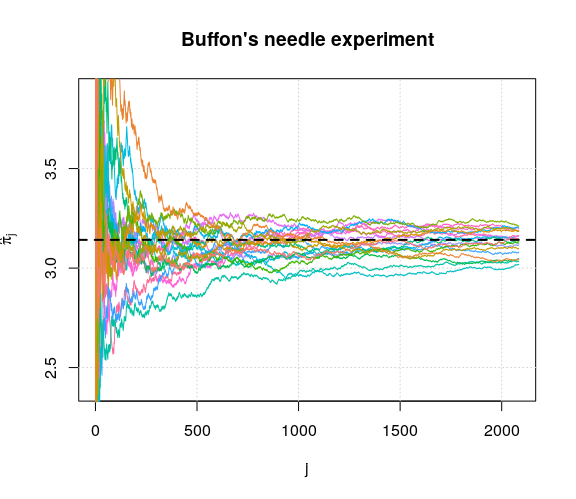
\includegraphics{ds_files/figure-latex/unnamed-chunk-241-1} \end{center}

which provides some illustrations on the convergence of the estimator.

\subsection{Step 2: Frontend}\label{step-2-frontend}

We start by constructing an ``empty'' Shiny app, i.e.

\begin{Shaded}
\begin{Highlighting}[]
\CommentTok{# Define UI for application}
\NormalTok{ui <-}\StringTok{ }\KeywordTok{fluidPage}\NormalTok{(}
  
  \CommentTok{# Application title}
  \KeywordTok{titlePanel}\NormalTok{(}\KeywordTok{h4}\NormalTok{(}\StringTok{"Buffon}\CharTok{\textbackslash{}'}\StringTok{s needle experiment - Inputs:"}\NormalTok{)),}
  
  \KeywordTok{sidebarLayout}\NormalTok{(}
    \KeywordTok{sidebarPanel}\NormalTok{(}
      \CommentTok{# Add inputs here!}
\NormalTok{    ),}
    
    \KeywordTok{mainPanel}\NormalTok{(}
      \KeywordTok{tabsetPanel}\NormalTok{(}
        \CommentTok{# Add tabs here!}
\NormalTok{      )}
\NormalTok{    )}
\NormalTok{  )}
\NormalTok{)}

\CommentTok{# Define server}
\NormalTok{server <-}\StringTok{ }\ControlFlowTok{function}\NormalTok{(input, output) \{}
\NormalTok{\}}

\CommentTok{# Run the application }
\KeywordTok{shinyApp}\NormalTok{(}\DataTypeTok{ui =}\NormalTok{ ui, }\DataTypeTok{server =}\NormalTok{ server)}
\end{Highlighting}
\end{Shaded}

If you run this empty app you should obtain the result below:

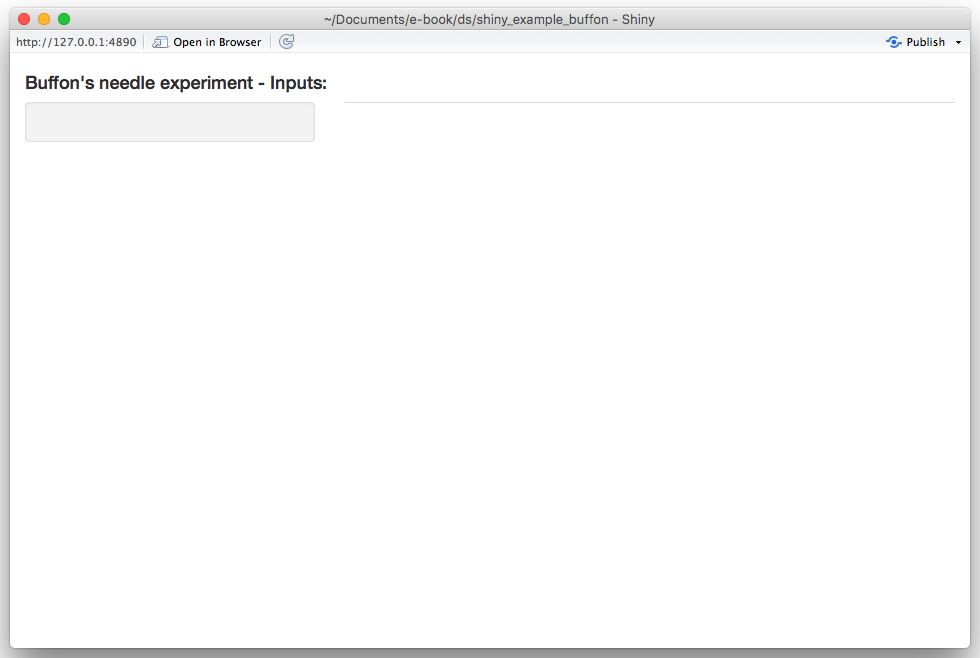
\includegraphics{images/shiny_ui_part1.png}

We will start by adding the required input widgets by modifying the
\texttt{ui} function as follows:

\begin{Shaded}
\begin{Highlighting}[]
\CommentTok{# Define UI for application}
\NormalTok{ui <-}\StringTok{ }\KeywordTok{fluidPage}\NormalTok{(}
  
  \CommentTok{# Application title}
  \KeywordTok{titlePanel}\NormalTok{(}\KeywordTok{h4}\NormalTok{(}\StringTok{"Buffon}\CharTok{\textbackslash{}'}\StringTok{s needle experiment - Inputs:"}\NormalTok{)),}
  
  \KeywordTok{sidebarLayout}\NormalTok{(}
    \KeywordTok{sidebarPanel}\NormalTok{(}
      \KeywordTok{numericInput}\NormalTok{(}\StringTok{"plane"}\NormalTok{, }\StringTok{"Plane width:"}\NormalTok{, }\DecValTok{10}\NormalTok{, }\DecValTok{6}\NormalTok{, }\DecValTok{100}\NormalTok{),}
      \KeywordTok{numericInput}\NormalTok{(}\StringTok{"B"}\NormalTok{, }\StringTok{"Number of trials:"}\NormalTok{, }\DecValTok{100}\NormalTok{, }\DecValTok{20}\NormalTok{, }\DecValTok{10}\OperatorTok{^}\DecValTok{6}\NormalTok{),}
      \KeywordTok{numericInput}\NormalTok{(}\StringTok{"M"}\NormalTok{, }\StringTok{"Number of experiments:"}\NormalTok{, }\DecValTok{1}\NormalTok{, }\DecValTok{1}\NormalTok{, }\DecValTok{100}\NormalTok{),}
      \KeywordTok{numericInput}\NormalTok{(}\StringTok{"seed"}\NormalTok{, }\StringTok{"Simulation seed"}\NormalTok{, }\DecValTok{1777}\NormalTok{, }\DecValTok{1}\NormalTok{, }\DecValTok{1000000}\NormalTok{),}
      \KeywordTok{actionButton}\NormalTok{(}\StringTok{"cast"}\NormalTok{, }\StringTok{"Let's cast some needles!"}\NormalTok{, }\DataTypeTok{icon =} \KeywordTok{icon}\NormalTok{(}\StringTok{"thumbs-up"}\NormalTok{))}
\NormalTok{    ),}
    
    \KeywordTok{mainPanel}\NormalTok{(}
      \KeywordTok{tabsetPanel}\NormalTok{(}
        \CommentTok{# Add tabs here!}
\NormalTok{      )}
\NormalTok{    )}
\NormalTok{  )}
\NormalTok{)}
\end{Highlighting}
\end{Shaded}

By running this update you should now obtain:

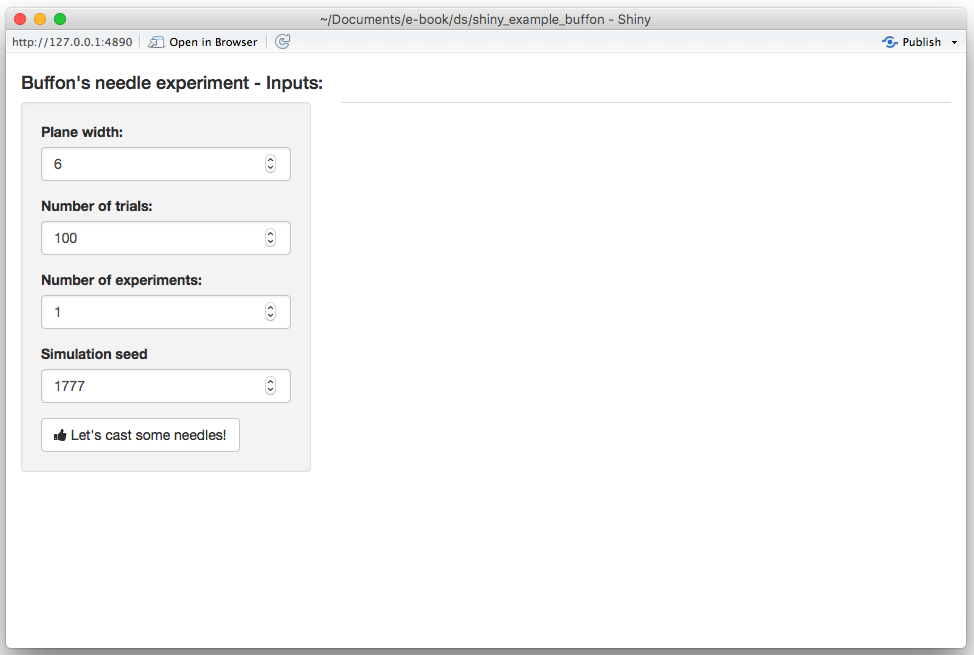
\includegraphics{images/shiny_ui_part2.png}

Next, we create two output tabs in which we will find the previously
mentioned graphs. This can be done by again modifying the
\texttt{ui}function as follows:

\begin{Shaded}
\begin{Highlighting}[]
\CommentTok{# Define UI for application}
\NormalTok{ui <-}\StringTok{ }\KeywordTok{fluidPage}\NormalTok{(}
  
  \CommentTok{# Application title}
  \KeywordTok{titlePanel}\NormalTok{(}\KeywordTok{h4}\NormalTok{(}\StringTok{"Buffon}\CharTok{\textbackslash{}'}\StringTok{s needle experiment - Inputs:"}\NormalTok{)),}
  
  \KeywordTok{sidebarLayout}\NormalTok{(}
    \KeywordTok{sidebarPanel}\NormalTok{(}
      \KeywordTok{numericInput}\NormalTok{(}\StringTok{"plane"}\NormalTok{, }\StringTok{"Plane width:"}\NormalTok{, }\DecValTok{10}\NormalTok{, }\DecValTok{6}\NormalTok{, }\DecValTok{100}\NormalTok{),}
      \KeywordTok{numericInput}\NormalTok{(}\StringTok{"B"}\NormalTok{, }\StringTok{"Number of trials:"}\NormalTok{, }\DecValTok{100}\NormalTok{, }\DecValTok{20}\NormalTok{, }\DecValTok{10}\OperatorTok{^}\DecValTok{6}\NormalTok{),}
      \KeywordTok{numericInput}\NormalTok{(}\StringTok{"M"}\NormalTok{, }\StringTok{"Number of experiments:"}\NormalTok{, }\DecValTok{1}\NormalTok{, }\DecValTok{1}\NormalTok{, }\DecValTok{100}\NormalTok{),}
      \KeywordTok{numericInput}\NormalTok{(}\StringTok{"seed"}\NormalTok{, }\StringTok{"Simulation seed"}\NormalTok{, }\DecValTok{1777}\NormalTok{, }\DecValTok{1}\NormalTok{, }\DecValTok{1000000}\NormalTok{),}
      \KeywordTok{actionButton}\NormalTok{(}\StringTok{"cast"}\NormalTok{, }\StringTok{"Let's cast some needles!"}\NormalTok{, }\DataTypeTok{icon =} \KeywordTok{icon}\NormalTok{(}\StringTok{"thumbs-up"}\NormalTok{))}
\NormalTok{    ),}
    
    \KeywordTok{mainPanel}\NormalTok{(}
      \KeywordTok{tabsetPanel}\NormalTok{(}
        \KeywordTok{tabPanel}\NormalTok{(}\StringTok{"Experiment"}\NormalTok{, }\KeywordTok{plotOutput}\NormalTok{(}\StringTok{"exp"}\NormalTok{)),}
        \KeywordTok{tabPanel}\NormalTok{(}\StringTok{"Convergence"}\NormalTok{, }\KeywordTok{plotOutput}\NormalTok{(}\StringTok{"conv"}\NormalTok{))}
\NormalTok{      )}
\NormalTok{    )}
\NormalTok{  )}
\NormalTok{)}
\end{Highlighting}
\end{Shaded}

The app should now look like this:

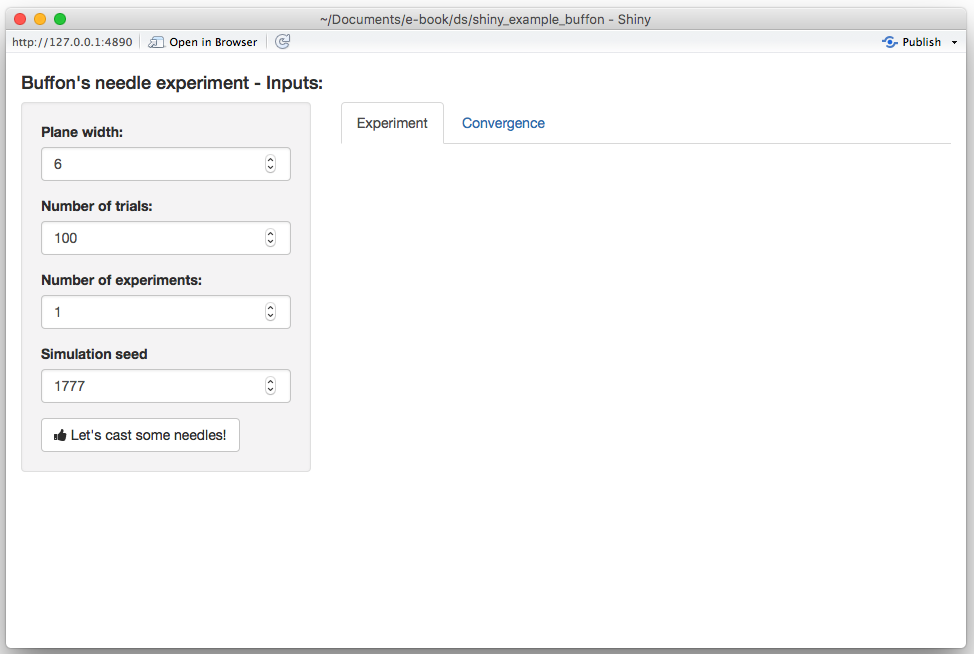
\includegraphics{images/shiny_ui_part3.png}

At this point, we have completed the \texttt{ui} function and will
modify the \texttt{server} in the next section.

\subsection{Step 3: Connecting frontend and
backend}\label{step-3-connecting-frontend-and-backend}

In this section, we will focus on the \texttt{server} function to
produce the desired output. Let us start by ``connecting'' our output
tabs defined in the \texttt{ui} function with the output in the server
function. Since both outputs are graphs, we will use the function
\texttt{renderPlot()} as follows:

\begin{Shaded}
\begin{Highlighting}[]
\NormalTok{server <-}\StringTok{ }\ControlFlowTok{function}\NormalTok{(input, output) \{}
\NormalTok{  output}\OperatorTok{$}\NormalTok{exp <-}\StringTok{ }\KeywordTok{renderPlot}\NormalTok{(\{}
    \CommentTok{# Add graph 1 here!}
\NormalTok{  \}, }\DataTypeTok{height =} \DecValTok{620}\NormalTok{)}
  
\NormalTok{  output}\OperatorTok{$}\NormalTok{conv <-}\StringTok{ }\KeywordTok{renderPlot}\NormalTok{(\{}
    \CommentTok{# Add graph 2 here!}
\NormalTok{  \}, }\DataTypeTok{height =} \DecValTok{620}\NormalTok{)}
\NormalTok{\}}
\end{Highlighting}
\end{Shaded}

If you re-run the app at this point our changes will have no visible
effect. Next, we will focus on the first graph based on the functions
\texttt{buffon\_experiment()} and \texttt{plot.buffon\_experiment()}.
The first thing we will need is to (re-)run the
\texttt{buffon\_experiment()} when the user clicks on the ``action''
button. This can be done by adding the following lines to the
\texttt{server} function:

\begin{Shaded}
\begin{Highlighting}[]
\NormalTok{cast <-}\StringTok{ }\KeywordTok{eventReactive}\NormalTok{(input}\OperatorTok{$}\NormalTok{cast, \{}
    \KeywordTok{buffon_experiment}\NormalTok{(}\DataTypeTok{B =}\NormalTok{ input}\OperatorTok{$}\NormalTok{B, }\DataTypeTok{plane_width =}\NormalTok{ input}\OperatorTok{$}\NormalTok{plane, }
                      \DataTypeTok{seed =}\NormalTok{ input}\OperatorTok{$}\NormalTok{seed)}
\NormalTok{  \})}
\end{Highlighting}
\end{Shaded}

When this function is (re-)evaluated we want to update/create the first
plot, which can be done by replacing the following part of the
\texttt{server} function

\begin{Shaded}
\begin{Highlighting}[]
\NormalTok{output}\OperatorTok{$}\NormalTok{exp <-}\StringTok{ }\KeywordTok{renderPlot}\NormalTok{(\{}
    \CommentTok{# Add graph 1 here!}
\NormalTok{\}, }\DataTypeTok{height =} \DecValTok{620}\NormalTok{)}
\end{Highlighting}
\end{Shaded}

with

\begin{Shaded}
\begin{Highlighting}[]
\NormalTok{output}\OperatorTok{$}\NormalTok{exp <-}\StringTok{ }\KeywordTok{renderPlot}\NormalTok{(\{}
    \KeywordTok{plot}\NormalTok{(}\KeywordTok{cast}\NormalTok{())}
\NormalTok{\}, }\DataTypeTok{height =} \DecValTok{620}\NormalTok{)}
\end{Highlighting}
\end{Shaded}

Therefore, your \texttt{server} function should now be:

\begin{Shaded}
\begin{Highlighting}[]
\NormalTok{server <-}\StringTok{ }\ControlFlowTok{function}\NormalTok{(input, output) \{}
  
  \CommentTok{# Fling some needles!}
\NormalTok{  cast <-}\StringTok{ }\KeywordTok{eventReactive}\NormalTok{(input}\OperatorTok{$}\NormalTok{cast, \{}
    \KeywordTok{buffon_experiment}\NormalTok{(}\DataTypeTok{B =}\NormalTok{ input}\OperatorTok{$}\NormalTok{B, }\DataTypeTok{plane_width =}\NormalTok{ input}\OperatorTok{$}\NormalTok{plane, }
                      \DataTypeTok{seed =}\NormalTok{ input}\OperatorTok{$}\NormalTok{seed)}
\NormalTok{  \})}
  
\NormalTok{  output}\OperatorTok{$}\NormalTok{exp <-}\StringTok{ }\KeywordTok{renderPlot}\NormalTok{(\{}
    \KeywordTok{plot}\NormalTok{(}\KeywordTok{cast}\NormalTok{())}
\NormalTok{  \}, }\DataTypeTok{height =} \DecValTok{620}\NormalTok{)}
  
\NormalTok{  output}\OperatorTok{$}\NormalTok{conv <-}\StringTok{ }\KeywordTok{renderPlot}\NormalTok{(\{}
    \CommentTok{# Add graph 2 here!}
\NormalTok{  \}, }\DataTypeTok{height =} \DecValTok{620}\NormalTok{)}
\NormalTok{\}}
\end{Highlighting}
\end{Shaded}

and when reloading the app you should now see:

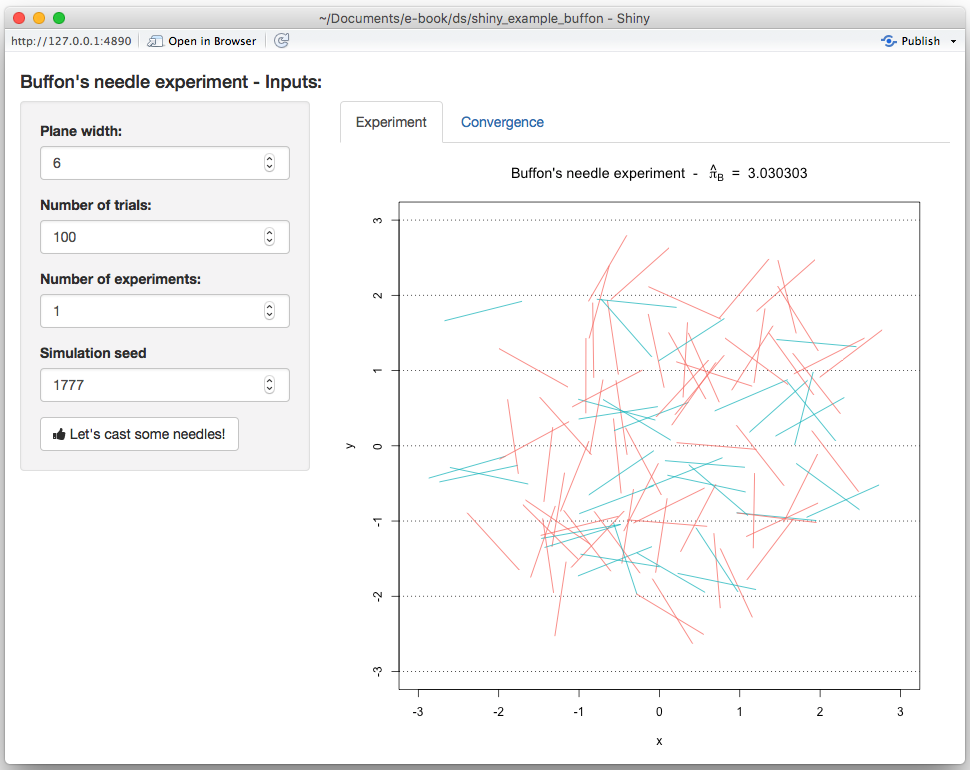
\includegraphics{images/shiny_server_part1.png}

Similarly, we do the same thing for the second graph by adding the
following lines to our \texttt{server} function:

\begin{Shaded}
\begin{Highlighting}[]
\NormalTok{conv <-}\StringTok{ }\KeywordTok{eventReactive}\NormalTok{(input}\OperatorTok{$}\NormalTok{cast, \{}
    \KeywordTok{converge}\NormalTok{(}\DataTypeTok{B =}\NormalTok{ input}\OperatorTok{$}\NormalTok{B, }\DataTypeTok{plane_width =}\NormalTok{ input}\OperatorTok{$}\NormalTok{plane, }
             \DataTypeTok{seed =}\NormalTok{ input}\OperatorTok{$}\NormalTok{seed, }\DataTypeTok{M =}\NormalTok{ input}\OperatorTok{$}\NormalTok{M)}
\NormalTok{\})}
\end{Highlighting}
\end{Shaded}

and replacing

\begin{Shaded}
\begin{Highlighting}[]
\NormalTok{output}\OperatorTok{$}\NormalTok{conv <-}\StringTok{ }\KeywordTok{renderPlot}\NormalTok{(\{}
    \CommentTok{# Add graph 2 here!}
\NormalTok{\}, }\DataTypeTok{height =} \DecValTok{620}\NormalTok{)}
\end{Highlighting}
\end{Shaded}

with

\begin{Shaded}
\begin{Highlighting}[]
\NormalTok{output}\OperatorTok{$}\NormalTok{conv <-}\StringTok{ }\KeywordTok{renderPlot}\NormalTok{(\{}
    \KeywordTok{conv}\NormalTok{()}
\NormalTok{\}, }\DataTypeTok{height =} \DecValTok{620}\NormalTok{)}
\end{Highlighting}
\end{Shaded}

After these changes, your \texttt{server} function should look like
this:

\begin{Shaded}
\begin{Highlighting}[]
\NormalTok{server <-}\StringTok{ }\ControlFlowTok{function}\NormalTok{(input, output) \{}
  
  \CommentTok{# Fling some needles!}
\NormalTok{  cast <-}\StringTok{ }\KeywordTok{eventReactive}\NormalTok{(input}\OperatorTok{$}\NormalTok{cast, \{}
    \KeywordTok{buffon_experiment}\NormalTok{(}\DataTypeTok{B =}\NormalTok{ input}\OperatorTok{$}\NormalTok{B, }\DataTypeTok{plane_width =}\NormalTok{ input}\OperatorTok{$}\NormalTok{plane, }
                      \DataTypeTok{seed =}\NormalTok{ input}\OperatorTok{$}\NormalTok{seed)}
\NormalTok{  \})}
  
\NormalTok{  conv <-}\StringTok{ }\KeywordTok{eventReactive}\NormalTok{(input}\OperatorTok{$}\NormalTok{cast, \{}
    \KeywordTok{converge}\NormalTok{(}\DataTypeTok{B =}\NormalTok{ input}\OperatorTok{$}\NormalTok{B, }\DataTypeTok{plane_width =}\NormalTok{ input}\OperatorTok{$}\NormalTok{plane, }
             \DataTypeTok{seed =}\NormalTok{ input}\OperatorTok{$}\NormalTok{seed, }\DataTypeTok{M =}\NormalTok{ input}\OperatorTok{$}\NormalTok{M)}
\NormalTok{  \})}
  
\NormalTok{  output}\OperatorTok{$}\NormalTok{exp <-}\StringTok{ }\KeywordTok{renderPlot}\NormalTok{(\{}
    \KeywordTok{plot}\NormalTok{(}\KeywordTok{cast}\NormalTok{())}
\NormalTok{  \}, }\DataTypeTok{height =} \DecValTok{620}\NormalTok{)}
  
\NormalTok{  output}\OperatorTok{$}\NormalTok{conv <-}\StringTok{ }\KeywordTok{renderPlot}\NormalTok{(\{}
    \KeywordTok{conv}\NormalTok{()}
\NormalTok{  \}, }\DataTypeTok{height =} \DecValTok{620}\NormalTok{)}
\NormalTok{\}}
\end{Highlighting}
\end{Shaded}

and when reloading the app you should now see on the second tab:

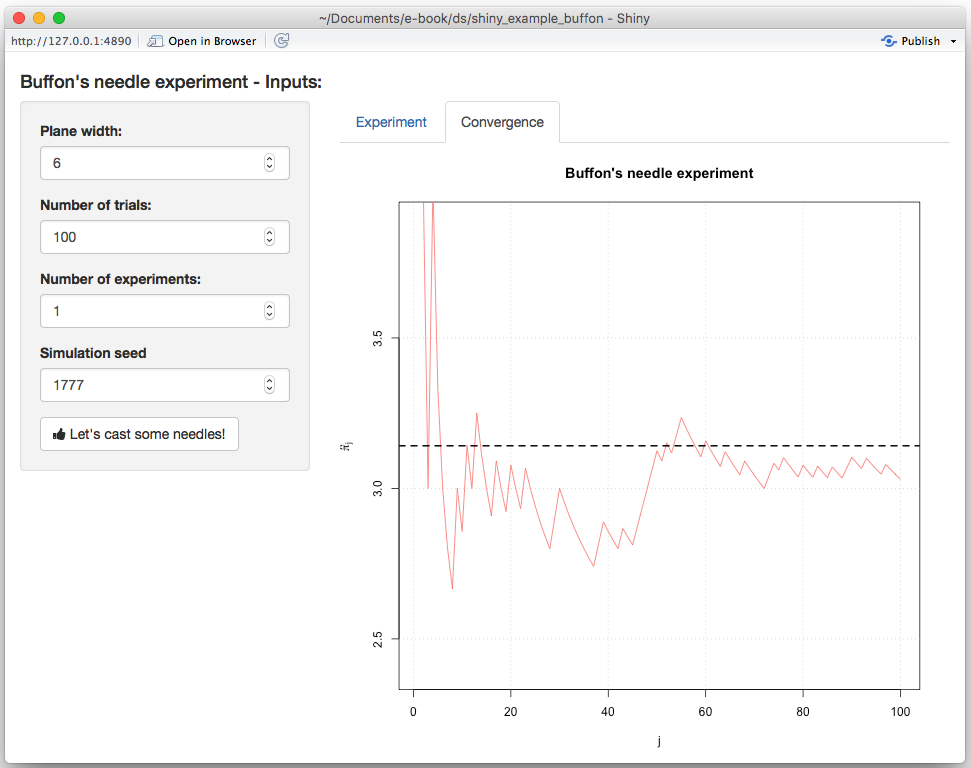
\includegraphics{images/shiny_server_part2.png}

Our next step is now to update the seed every time the ``action'' button
is pushed. To do so, we will first need to add an additional input to
the \texttt{server} function called \texttt{session} which will allow us
to \textbf{dynamically} update the input directly from the
\texttt{server} function. Therefore, in order to randomly generate a new
seed each time the user clicks on the ``action'' button, we can do the
following:

\begin{Shaded}
\begin{Highlighting}[]
\KeywordTok{observeEvent}\NormalTok{(input}\OperatorTok{$}\NormalTok{cast,\{}
    \KeywordTok{updateNumericInput}\NormalTok{(session, }\StringTok{"seed"}\NormalTok{, }
                       \DataTypeTok{value =} \KeywordTok{round}\NormalTok{(}\KeywordTok{runif}\NormalTok{(}\DecValTok{1}\NormalTok{, }\DecValTok{1}\NormalTok{, }\DecValTok{10}\OperatorTok{^}\DecValTok{4}\NormalTok{)))}
\NormalTok{\})}
\end{Highlighting}
\end{Shaded}

Therefore, your final \texttt{server} function is now:

\begin{Shaded}
\begin{Highlighting}[]
\NormalTok{server <-}\StringTok{ }\ControlFlowTok{function}\NormalTok{(input, output, session) \{}
  
  \KeywordTok{observeEvent}\NormalTok{(input}\OperatorTok{$}\NormalTok{cast,\{}
    \KeywordTok{updateNumericInput}\NormalTok{(session, }\StringTok{"seed"}\NormalTok{, }
                       \DataTypeTok{value =} \KeywordTok{round}\NormalTok{(}\KeywordTok{runif}\NormalTok{(}\DecValTok{1}\NormalTok{, }\DecValTok{1}\NormalTok{, }\DecValTok{10}\OperatorTok{^}\DecValTok{4}\NormalTok{)))}
\NormalTok{  \})}
  
  \CommentTok{# Fling some needles!}
\NormalTok{  cast =}\StringTok{ }\KeywordTok{eventReactive}\NormalTok{(input}\OperatorTok{$}\NormalTok{cast, \{}
    \KeywordTok{buffon_experiment}\NormalTok{(}\DataTypeTok{B =}\NormalTok{ input}\OperatorTok{$}\NormalTok{B, }\DataTypeTok{plane_width =}\NormalTok{ input}\OperatorTok{$}\NormalTok{plane, }
                      \DataTypeTok{seed =}\NormalTok{ input}\OperatorTok{$}\NormalTok{seed)}
\NormalTok{  \})}
  
\NormalTok{  conv =}\StringTok{ }\KeywordTok{eventReactive}\NormalTok{(input}\OperatorTok{$}\NormalTok{cast, \{}
    \KeywordTok{converge}\NormalTok{(}\DataTypeTok{B =}\NormalTok{ input}\OperatorTok{$}\NormalTok{B, }\DataTypeTok{plane_width =}\NormalTok{ input}\OperatorTok{$}\NormalTok{plane, }
             \DataTypeTok{seed =}\NormalTok{ input}\OperatorTok{$}\NormalTok{seed, }\DataTypeTok{M =}\NormalTok{ input}\OperatorTok{$}\NormalTok{M)}
\NormalTok{  \})}
  
\NormalTok{  output}\OperatorTok{$}\NormalTok{exp <-}\StringTok{ }\KeywordTok{renderPlot}\NormalTok{(\{}
    \KeywordTok{plot}\NormalTok{(}\KeywordTok{cast}\NormalTok{())}
\NormalTok{  \}, }\DataTypeTok{height =} \DecValTok{620}\NormalTok{)}
  
\NormalTok{  output}\OperatorTok{$}\NormalTok{conv <-}\StringTok{ }\KeywordTok{renderPlot}\NormalTok{(\{}
    \KeywordTok{conv}\NormalTok{()}
\NormalTok{  \}, }\DataTypeTok{height =} \DecValTok{620}\NormalTok{)}
\NormalTok{\}}
\end{Highlighting}
\end{Shaded}

With this change, you will now observe that the seed is updated each
time the ``action'' button is clicked. The final version of the app we
have just created can be found
\href{http://shiny.science.psu.edu/szg279/buffon/}{here}.

\chapter{R Packages}\label{r-packages}

In this chapter we introduce one of the most useful tools for R
programming as well as for statistical programming in general. Indeed,
one of the main goals for statistical programming is to then be able to
share all the code and functions that have been implemented in order to
respond to a specific task. The latter may often be quite \emph{messy}
to do given that different files and functions can be present in various
directories or repositories and, for example, some codes may use
functions from other codes but do not load the same libraries, thereby
producing execution errors.

In order to avoid the above complications (and to program in a healthy
and organized manner), R allows you to create \emph{packages} that are
software platforms that collect functions as well as other files which,
among others, describe these functions and provide users with
documentation that allow them to understand and efficiently use these
functions. Moreover, when sharing a package (or making it available
within a repository) all the user needs to do is to install and load the
package within an R session which then makes available the entire
environment needed for all the functions included in the package to
work. In a nutshell, whenever creating functions to answer a specific
research interest or professional task, it is always good to do so by
first creating a package within which these functions can be stored and
documented.

In this chapter we will describe and explain the steps necessary to
create an R package using RStudio. There are other ways and other
procedures to produce an R package but in this chapter we will describe
one possible way which is consistent with the approach to statistical
programming that is presented in this book. As in the previous chapters,
we will make use of an example to guide the reader through the different
aspects of package building and, for this purpose, let us assume we want
to build a package that allows a user to perform Monte-Carlo integration
for any user-specificed function as well as produce plots that represent
these functions as well as the integrated area. In this case, we have an
extremely simple setting where, based on code used in the previous
chapters, we only have the following two functions to be included in the
package:

\begin{Shaded}
\begin{Highlighting}[]
\NormalTok{mc_int =}\StringTok{ }\ControlFlowTok{function}\NormalTok{(x_range, fun, B, }\DataTypeTok{seed =} \DecValTok{1291}\NormalTok{)\{}
  \CommentTok{# A few checks}
  \CommentTok{# Check x_range}
  \ControlFlowTok{if}\NormalTok{ (}\KeywordTok{length}\NormalTok{(x_range) }\OperatorTok{!=}\StringTok{ }\DecValTok{2} \OperatorTok{||}\StringTok{ }\NormalTok{x_range[}\DecValTok{1}\NormalTok{] }\OperatorTok{>=}\StringTok{ }\NormalTok{x_range[}\DecValTok{2}\NormalTok{])\{}
    \KeywordTok{stop}\NormalTok{(}\StringTok{"x_range is incorrectly specified"}\NormalTok{)}
\NormalTok{  \}}

  \CommentTok{# Check fun}
  \ControlFlowTok{if}\NormalTok{ (}\KeywordTok{class}\NormalTok{(fun) }\OperatorTok{!=}\StringTok{ "character"}\NormalTok{)\{}
    \KeywordTok{stop}\NormalTok{(}\StringTok{"fun is incorrectly specified and should be a character"}\NormalTok{)}
\NormalTok{  \}}

\NormalTok{  x =}\StringTok{ }\KeywordTok{mean}\NormalTok{(x_range)}
\NormalTok{  test_fun =}\StringTok{ }\KeywordTok{try}\NormalTok{(}\KeywordTok{eval}\NormalTok{(}\KeywordTok{parse}\NormalTok{(}\DataTypeTok{text =}\NormalTok{ fun)), }\DataTypeTok{silent =} \OtherTok{TRUE}\NormalTok{)}
  \ControlFlowTok{if}\NormalTok{ (}\KeywordTok{class}\NormalTok{(test_fun) }\OperatorTok{==}\StringTok{ "try-error"}\NormalTok{)\{}
    \KeywordTok{stop}\NormalTok{(}\StringTok{"fun cannot be evaluated"}\NormalTok{)}
\NormalTok{  \}}

  \CommentTok{# Check B}
  \ControlFlowTok{if}\NormalTok{ (B }\OperatorTok{<}\StringTok{ }\DecValTok{1}\NormalTok{)\{}
    \KeywordTok{error}\NormalTok{(}\StringTok{"B is incorrectly specified"}\NormalTok{)}
\NormalTok{  \}}

  \CommentTok{# Set seed}
  \KeywordTok{set.seed}\NormalTok{(seed)}

  \CommentTok{# Compute the length of the interval, i.e. (b-a)}
\NormalTok{  interval_length =}\StringTok{ }\KeywordTok{diff}\NormalTok{(x_range)}

  \CommentTok{# Let's draw some uniforms to get Ui and Xi}
\NormalTok{  Ui =}\StringTok{ }\KeywordTok{runif}\NormalTok{(B)}
\NormalTok{  Xi =}\StringTok{ }\NormalTok{x_range[}\DecValTok{1}\NormalTok{] }\OperatorTok{+}\StringTok{ }\NormalTok{Ui}\OperatorTok{*}\NormalTok{interval_length}

  \CommentTok{# Compute \textbackslash{}hat\{I\}}
\NormalTok{  x =}\StringTok{ }\NormalTok{Xi}
\NormalTok{  I_hat =}\StringTok{ }\NormalTok{interval_length}\OperatorTok{*}\KeywordTok{mean}\NormalTok{(}\KeywordTok{eval}\NormalTok{(}\KeywordTok{parse}\NormalTok{(}\DataTypeTok{text =}\NormalTok{ fun)))}

  \CommentTok{# Compute \textbackslash{}hat\{I\}_2}
\NormalTok{  I2_hat =}\StringTok{ }\NormalTok{interval_length}\OperatorTok{*}\KeywordTok{mean}\NormalTok{((}\KeywordTok{eval}\NormalTok{(}\KeywordTok{parse}\NormalTok{(}\DataTypeTok{text =}\NormalTok{ fun)))}\OperatorTok{^}\DecValTok{2}\NormalTok{)}
\NormalTok{  var_I_hat =}\StringTok{ }\NormalTok{(interval_length}\OperatorTok{*}\NormalTok{I2_hat }\OperatorTok{-}\StringTok{ }\NormalTok{I_hat}\OperatorTok{^}\DecValTok{2}\NormalTok{)}\OperatorTok{/}\NormalTok{B}

  \CommentTok{# Output list}
\NormalTok{  out =}\StringTok{ }\KeywordTok{list}\NormalTok{(}\DataTypeTok{I =}\NormalTok{ I_hat, }\DataTypeTok{var =}\NormalTok{ var_I_hat,}
             \DataTypeTok{fun =}\NormalTok{ fun, }\DataTypeTok{x_range =}\NormalTok{ x_range, }\DataTypeTok{B =}\NormalTok{ B)}
  \KeywordTok{class}\NormalTok{(out) =}\StringTok{ "MCI"}
\NormalTok{  out}
\NormalTok{\}}

\NormalTok{plot.MCI =}\StringTok{ }\ControlFlowTok{function}\NormalTok{(x, ...)\{}
\NormalTok{  obj =}\StringTok{ }\NormalTok{x}
\NormalTok{  x_range =}\StringTok{ }\NormalTok{obj}\OperatorTok{$}\NormalTok{x_range}
\NormalTok{  fun =}\StringTok{ }\NormalTok{obj}\OperatorTok{$}\NormalTok{fun}

\NormalTok{  Delta =}\StringTok{ }\KeywordTok{diff}\NormalTok{(x_range)}
\NormalTok{  x_range_graph =}\StringTok{ }\KeywordTok{c}\NormalTok{(x_range[}\DecValTok{2}\NormalTok{] }\OperatorTok{-}\StringTok{ }\FloatTok{1.15}\OperatorTok{*}\NormalTok{Delta, x_range[}\DecValTok{1}\NormalTok{] }\OperatorTok{+}\StringTok{ }\FloatTok{1.15}\OperatorTok{*}\NormalTok{Delta)}
\NormalTok{  x =}\StringTok{ }\KeywordTok{seq}\NormalTok{(}\DataTypeTok{from =}\NormalTok{ x_range_graph[}\DecValTok{1}\NormalTok{], }\DataTypeTok{to =}\NormalTok{ x_range_graph[}\DecValTok{2}\NormalTok{], }\DataTypeTok{length.out =} \DecValTok{10}\OperatorTok{^}\DecValTok{3}\NormalTok{)}
\NormalTok{  f_x =}\StringTok{ }\KeywordTok{eval}\NormalTok{(}\KeywordTok{parse}\NormalTok{(}\DataTypeTok{text =}\NormalTok{ fun))}
  \KeywordTok{plot}\NormalTok{(}\OtherTok{NA}\NormalTok{, }\DataTypeTok{xlim =} \KeywordTok{range}\NormalTok{(x), }\DataTypeTok{ylim =} \KeywordTok{range}\NormalTok{(f_x), }\DataTypeTok{xlab =} \StringTok{"x"}\NormalTok{, }\DataTypeTok{ylab =} \StringTok{"f(x)"}\NormalTok{)}
  \KeywordTok{grid}\NormalTok{()}
  \KeywordTok{title}\NormalTok{(}\KeywordTok{paste}\NormalTok{(}\StringTok{"Estimated integral: "}\NormalTok{, }\KeywordTok{round}\NormalTok{(obj}\OperatorTok{$}\NormalTok{I,}\DecValTok{4}\NormalTok{),}
              \StringTok{" ("}\NormalTok{, }\KeywordTok{round}\NormalTok{(}\KeywordTok{sqrt}\NormalTok{(obj}\OperatorTok{$}\NormalTok{var),}\DecValTok{4}\NormalTok{),}\StringTok{")"}\NormalTok{, }\DataTypeTok{sep =} \StringTok{""}\NormalTok{))}
  \KeywordTok{lines}\NormalTok{(x, f_x)}
\NormalTok{  x =}\StringTok{ }\KeywordTok{seq}\NormalTok{(}\DataTypeTok{from =}\NormalTok{ x_range[}\DecValTok{1}\NormalTok{], }\DataTypeTok{to =}\NormalTok{ x_range[}\DecValTok{2}\NormalTok{], }\DataTypeTok{length.out =} \DecValTok{10}\OperatorTok{^}\DecValTok{3}\NormalTok{)}
\NormalTok{  f_x =}\StringTok{ }\KeywordTok{eval}\NormalTok{(}\KeywordTok{parse}\NormalTok{(}\DataTypeTok{text =}\NormalTok{ fun))}
\NormalTok{  cols =}\StringTok{ }\KeywordTok{hcl}\NormalTok{(}\DataTypeTok{h =} \KeywordTok{seq}\NormalTok{(}\DecValTok{15}\NormalTok{, }\DecValTok{375}\NormalTok{, }\DataTypeTok{length =} \DecValTok{3}\NormalTok{), }\DataTypeTok{l =} \DecValTok{65}\NormalTok{, }\DataTypeTok{c =} \DecValTok{100}\NormalTok{, }\DataTypeTok{alpha =} \FloatTok{0.4}\NormalTok{)[}\DecValTok{1}\OperatorTok{:}\DecValTok{3}\NormalTok{]}
  \KeywordTok{polygon}\NormalTok{(}\KeywordTok{c}\NormalTok{(x, }\KeywordTok{rev}\NormalTok{(x)), }\KeywordTok{c}\NormalTok{(}\KeywordTok{rep}\NormalTok{(}\DecValTok{0}\NormalTok{, }\KeywordTok{length}\NormalTok{(x)), }\KeywordTok{rev}\NormalTok{(f_x)),}
          \DataTypeTok{border =} \OtherTok{NA}\NormalTok{, }\DataTypeTok{col =}\NormalTok{ cols[}\DecValTok{1}\NormalTok{])}
  \KeywordTok{abline}\NormalTok{(}\DataTypeTok{v =}\NormalTok{ x_range[}\DecValTok{1}\NormalTok{], }\DataTypeTok{lty =} \DecValTok{2}\NormalTok{)}
  \KeywordTok{abline}\NormalTok{(}\DataTypeTok{v =}\NormalTok{ x_range[}\DecValTok{2}\NormalTok{], }\DataTypeTok{lty =} \DecValTok{2}\NormalTok{)}
\NormalTok{\}}
\end{Highlighting}
\end{Shaded}

Hence, the package will contain:

\begin{itemize}
\tightlist
\item
  the \texttt{mc\_int()} function: that computes an approximation of the
  integral of the function \texttt{fun} with respect to \texttt{x}
  within the range \texttt{x\_range} via Monte-Carlo integration using
  uniform sampling;
\item
  the \texttt{plot.MCI()} function: a class function that will plot the
  object that is created as an output of the \texttt{mc\_int()}
  function.
\end{itemize}

An example of use of these functions and their output is the following:

\begin{Shaded}
\begin{Highlighting}[]
\NormalTok{obj =}\StringTok{ }\KeywordTok{mc_int}\NormalTok{(}\DataTypeTok{x_range =} \KeywordTok{c}\NormalTok{(}\DecValTok{0}\NormalTok{,}\DecValTok{1}\NormalTok{), }\DataTypeTok{fun =} \StringTok{"x^2*sin(x^2/pi)"}\NormalTok{, }\DataTypeTok{B =} \DecValTok{10}\OperatorTok{^}\DecValTok{3}\NormalTok{)}
\KeywordTok{plot}\NormalTok{(obj)}
\end{Highlighting}
\end{Shaded}

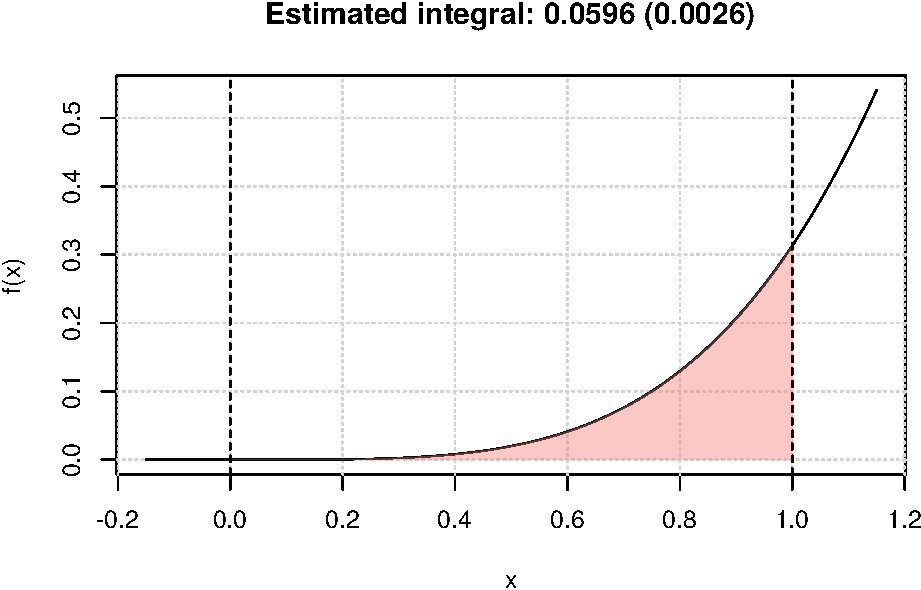
\includegraphics{ds_files/figure-latex/unnamed-chunk-257-1.pdf}

Now let us suppose that we want to make these functions available to the
general user who may be looking for tools that allow them to perform
Monte-Carlo intergration. Although we only have two functions, it would
be appropriate to provide a single platform containing these functions
along with documentation that describes the contents and use of these
functions. Therefore, in the following sections we will describe the
process to develop an R package for these functions which is consquently
valid for any collection of functions needed to perform a specific task.

\section{Basic steps}\label{basic-steps}

As mentioned earlier, the process to develop an R package that is
described in this chapter is not strict or unique since there are many
different ways of structuring and building them. However, in this book
we will describe one way of building a package which is consistent with
the approach to statistical programming that has been described thus
far. Keeping this in mind, below the reader can find the basic steps to
build an R package.

\subsection{\texorpdfstring{Step 1: Create an ``empty'' R
package}{Step 1: Create an empty R package}}\label{step-1-create-an-empty-r-package}

The first step to create an R package using RStudio is to build the
\emph{skeleton} of the package which contains the basic folders and
files that are needed. To do so, within RStudio you should select to
create a ``New Project\ldots{}'' from the File menu within RStudio as
shown below.

\includegraphics{images/part1_1.png}

Once this is done you will see a new window with different options (see
image below) among which you select ``New Directory'' (unless you wish
to create the package within an existing directory which is usually not
convenient for purpose of organization).

\includegraphics{images/part1_2.png}

Again, another window will appear in which RStudio asks you for the type
of project you wish to create and, quite intuitively, you should select
the ``R Package'' option as shown below.

\includegraphics{images/part1_3.png}

By doing so you prompt a successive window in which it is possible to
name our package which, in the example below, will be \texttt{demo}. In
the context of this chapter we will not consider the other options that
are made available to the user (for more details you can check
\href{http://r-pkgs.had.co.nz/}{this link}).

\includegraphics{images/part1_4.png}

Once the package has been named, you can select ``Create Project'' and
another window will be prompted in which the basic files and folders
needed for a package will be visualized within an overall repository
with the same name as the package (i.e. ``demo'') as shown below.

\includegraphics{images/part2_1.png}

Within the logic of this chapter which provides one possible procedure
(out of various) to build an R package, we will proceed to removing the
following files from this folder:

\begin{itemize}
\tightlist
\item
  NAMESPACE
\item
  man/hello.Rd
\item
  R/hello.R
\end{itemize}

These files are default functions and documentation that are created to
provide a basis for the user who can then modify them using their own
descriptions and functions. However, for the procedure described in this
chapter their presence is redundant (as seen further on) and
consequently we invite the reader to remove them if they decide to
follow the steps described in this chapter.

\subsection{Step 2: Edit description
file}\label{step-2-edit-description-file}

This first step hence creates the skeleton of the package and, in the
following steps, we can focus on giving body to this skeleton, starting
from the file which contains a summary description of the structure and
contents of the package which is to be found in the ``DESCRIPTION''
file. Once this is opened the user will notice different parts to this
file in which various information on the package is contained such as
the package name, author information, license and imports. Although
there are other pieces of information (see
\href{http://r-pkgs.had.co.nz/description.html}{this link}), we will
quickly discuss the latter three in the following paragraphs.

\subsubsection*{Author Roles}\label{author-roles}


One of the lines of information in the description file corresponds to
the authors of the package. This therefore corresponds to the list of
persons who have actively contributed to the development of code and
functions that are included in the package. When there is more than
author, the line corresponding to the author can be replaced by a format
like the following:

\begin{Shaded}
\begin{Highlighting}[]
\NormalTok{Authors}\OperatorTok{@}\NormalTok{R}\OperatorTok{:}\StringTok{ }\KeywordTok{c}\NormalTok{(}
    \KeywordTok{person}\NormalTok{(}\StringTok{"Justin"}\NormalTok{, }\StringTok{"Lee"}\NormalTok{, }\DataTypeTok{email =} \StringTok{"justinlee@psu.edu"}\NormalTok{, }\DataTypeTok{role =} \KeywordTok{c}\NormalTok{(}\StringTok{"aut"}\NormalTok{,}\StringTok{"cre"}\NormalTok{)),}
    \KeywordTok{person}\NormalTok{(}\StringTok{"Stephane"}\NormalTok{, }\StringTok{"Guerrier"}\NormalTok{, }\DataTypeTok{role =} \StringTok{"aut"}\NormalTok{),}
    \KeywordTok{person}\NormalTok{(}\StringTok{"Roberto"}\NormalTok{, }\StringTok{"Molinari"}\NormalTok{, }\DataTypeTok{role =} \StringTok{"aut"}\NormalTok{),}
    \KeywordTok{person}\NormalTok{(}\StringTok{"Matthew"}\NormalTok{, }\StringTok{"Beckman"}\NormalTok{, }\DataTypeTok{role =} \StringTok{"aut"}\NormalTok{)}
\NormalTok{    )}
\end{Highlighting}
\end{Shaded}

This information is important also because it will impact how it is
displayed later in the rendered package website (see further on). As you
can notice it possible to also specify the role that the author has in
relation to the package using the option \texttt{role\ =}, followed by
codes for the type of role. In the above examples we can see two types
of role that correspond to \texttt{aut} which indicates an \emph{author}
of the package while \texttt{cre} stands for \emph{creator} who is the
person in charge of maintaining the package and receiving information as
well as bug reports or suggestions. There are other two possible roles
available which are \texttt{ctb} and \texttt{cph} that correspond to
\emph{contributor} and \emph{copyright holder} respectively, where the
contributor is a person who has provided some minor contributions to the
package while the copyright holder is the person or company who holds
the copyright of the package.

\subsubsection*{License}\label{license-1}


The package license determines to what extent and under what conditions
the package (and its contents) can be shared and accessed by users. The
most common license is the GNU General Public License which is a widely
used free software license that guarantees end-users the possibility to
run, study, share and modify the software. A complete list of all the
possible licenses can be found at this
\href{https://cran.r-project.org/web/licenses/}{link} and you are free
to choose the license that best fits your requirements.

\subsubsection*{Imports}\label{imports}


It is often the case that your code and functions will depend on
functions that are made available from other packages in R. In order to
make sure that these packages are available to the user when they
install your package, it is important to specify on which external
packages yours relies on. In this sense, the \texttt{Imports} line in
the DESCRIPTION file allows you to do just this so it is important to
remember to check whether external packages are correctly specified in
this section of the file.

Our example on Monte-Carlo integration only depends on the base
functions in R and therefore there is no need to specify external
packages for this case. Therefore, our ``demo'' package DESCRIPTION file
ends up looking as follows:

\includegraphics{images/description.png}

\subsection{Step 3: Move your R scripts into the R
folder}\label{step-3-move-your-r-scripts-into-the-r-folder}

Having completed the description of the package we can now focus on
adding the truly essential part of the package: the functions that
deliver the outputs required by the user. In order for the functions to
be considered as part of the package, the scripts containing these
functions need to be moved into the R folder that is created as part of
the package skeleton as seen earlier (therefore replacing the
``hello.R'' script that we chose to delete).

The organization of the code that collects the functions is subjective
and can be included all in one single R script or in various scripts. It
is usually suggested to group these functions into separate scripts
according to their relative themes or specific tasks they are created
for, especially when there is a considerable number of functions in the
package. This approach allows to more easily find and fix any errors
that are present in the functions as opposed to going through thousands
of lines of code to find the function you're interested in.

In our example we only have two functions so there is no need to
separate them and, consequently, we include them in a single R script
that we call ``mc\_integration.R'' which is included in the R folder for
our demo package.

\includegraphics{images/r_code.png}

As you may notice, there is another file called ``run\_shiny.R'' which,
as we will see later, contains the code to create a Shiny app that is
part of the package.

\subsection{Step 4: Documentation}\label{step-4-documentation}

The next essential component of a package is its documentation which
enables users to know how to use it. Indeed, when users access the
\texttt{demo} package, they should essentially know how to use its
functions by gaining access to help files through the use of commands
like \texttt{?mc\_int} for example. A possible (and efficient) way of
creating package documentation is by using a specific syntax before each
function in your R scripts which will then be used to automatically
generate the necessary \texttt{.Rd} files by using the commands
\texttt{devtools::document()} or \texttt{roxygen2::roxygenize}.

We will use the \texttt{mc\_int()} function from our demo package as an
example to show the syntax that can be used before each function which
is intended for the user:

\begin{Shaded}
\begin{Highlighting}[]
\CommentTok{#' @title Simple Monte-Carlo integration}
\CommentTok{#'}
\CommentTok{#' @description Compute an approximation of the integral of the function f(x)}
\CommentTok{#' with respect to dx in the range [a, b] by Monte-Carlo integration using}
\CommentTok{#' uniform sampling.}
\CommentTok{#' @param x_range A \textbackslash{}code\{vector\} of dimension 2 used to denote the integration}
\CommentTok{#' region of interest, i.e. [a, b].}
\CommentTok{#' @param fun A \textbackslash{}code\{string\} containing the function to be integrated. It}
\CommentTok{#' is assumed that \textbackslash{}code\{x\} is used as the variable of interest.}
\CommentTok{#' @param B A \textbackslash{}code\{numeric\} (integer) used to denote the number of simulations.}
\CommentTok{#' @param seed A \textbackslash{}code\{numeric\} used to control the seed of the random number}
\CommentTok{#' generator used by this function.}
\CommentTok{#' @return A \textbackslash{}code\{list\} containing the following attributes:}
\CommentTok{#' \textbackslash{}describe\{}
\CommentTok{#'      \textbackslash{}item\{I\}\{Estimated value of the integral\}}
\CommentTok{#'      \textbackslash{}item\{var\}\{Estimated variance of the estimator\}}
\CommentTok{#' \}}
\CommentTok{#' @author Stephane Guerrier}
\CommentTok{#' @importFrom stats runif}
\CommentTok{#' @export}
\CommentTok{#' @examples}
\CommentTok{#' mc_int(x_range = c(0,1), fun = "x^2", B = 10^5)}
\CommentTok{#' mc_int(x_range = c(0,1), fun = "x^2*sin(x^2/pi)", B = 10^5)}
\NormalTok{mc_int =}\StringTok{ }\ControlFlowTok{function}\NormalTok{(x_range, fun, B, }\DataTypeTok{seed =} \DecValTok{1291}\NormalTok{)\{}
  \CommentTok{# A few checks}
  \CommentTok{# Check x_range}
  \ControlFlowTok{if}\NormalTok{ (}\KeywordTok{length}\NormalTok{(x_range) }\OperatorTok{!=}\StringTok{ }\DecValTok{2} \OperatorTok{||}\StringTok{ }\NormalTok{x_range[}\DecValTok{1}\NormalTok{] }\OperatorTok{>=}\StringTok{ }\NormalTok{x_range[}\DecValTok{2}\NormalTok{])\{}
    \KeywordTok{stop}\NormalTok{(}\StringTok{"x_range is incorrectly specified"}\NormalTok{)}
\NormalTok{  \}}

  \CommentTok{# Check fun}
  \ControlFlowTok{if}\NormalTok{ (}\KeywordTok{class}\NormalTok{(fun) }\OperatorTok{!=}\StringTok{ "character"}\NormalTok{)\{}
    \KeywordTok{stop}\NormalTok{(}\StringTok{"fun is incorrectly specified and should be a character"}\NormalTok{)}
\NormalTok{  \}}

\NormalTok{  x =}\StringTok{ }\KeywordTok{mean}\NormalTok{(x_range)}
\NormalTok{  test_fun =}\StringTok{ }\KeywordTok{try}\NormalTok{(}\KeywordTok{eval}\NormalTok{(}\KeywordTok{parse}\NormalTok{(}\DataTypeTok{text =}\NormalTok{ fun)), }\DataTypeTok{silent =} \OtherTok{TRUE}\NormalTok{)}
  \ControlFlowTok{if}\NormalTok{ (}\KeywordTok{class}\NormalTok{(test_fun) }\OperatorTok{==}\StringTok{ "try-error"}\NormalTok{)\{}
    \KeywordTok{stop}\NormalTok{(}\StringTok{"fun cannot be evaluated"}\NormalTok{)}
\NormalTok{  \}}

  \CommentTok{# Check B}
  \ControlFlowTok{if}\NormalTok{ (B }\OperatorTok{<}\StringTok{ }\DecValTok{1}\NormalTok{)\{}
    \KeywordTok{error}\NormalTok{(}\StringTok{"B is incorrectly specified"}\NormalTok{)}
\NormalTok{  \}}

  \CommentTok{# Set seed}
  \KeywordTok{set.seed}\NormalTok{(seed)}

  \CommentTok{# Compute the length of the interval, i.e. (b-a)}
\NormalTok{  interval_length =}\StringTok{ }\KeywordTok{diff}\NormalTok{(x_range)}

  \CommentTok{# Let's draw some uniforms to get Ui and Xi}
\NormalTok{  Ui =}\StringTok{ }\KeywordTok{runif}\NormalTok{(B)}
\NormalTok{  Xi =}\StringTok{ }\NormalTok{x_range[}\DecValTok{1}\NormalTok{] }\OperatorTok{+}\StringTok{ }\NormalTok{Ui}\OperatorTok{*}\NormalTok{interval_length}

  \CommentTok{# Compute \textbackslash{}hat\{I\}}
\NormalTok{  x =}\StringTok{ }\NormalTok{Xi}
\NormalTok{  I_hat =}\StringTok{ }\NormalTok{interval_length}\OperatorTok{*}\KeywordTok{mean}\NormalTok{(}\KeywordTok{eval}\NormalTok{(}\KeywordTok{parse}\NormalTok{(}\DataTypeTok{text =}\NormalTok{ fun)))}

  \CommentTok{# Compute \textbackslash{}hat\{I\}_2}
\NormalTok{  I2_hat =}\StringTok{ }\NormalTok{interval_length}\OperatorTok{*}\KeywordTok{mean}\NormalTok{((}\KeywordTok{eval}\NormalTok{(}\KeywordTok{parse}\NormalTok{(}\DataTypeTok{text =}\NormalTok{ fun)))}\OperatorTok{^}\DecValTok{2}\NormalTok{)}
\NormalTok{  var_I_hat =}\StringTok{ }\NormalTok{(interval_length}\OperatorTok{*}\NormalTok{I2_hat }\OperatorTok{-}\StringTok{ }\NormalTok{I_hat}\OperatorTok{^}\DecValTok{2}\NormalTok{)}\OperatorTok{/}\NormalTok{B}

  \CommentTok{# Output list}
\NormalTok{  out =}\StringTok{ }\KeywordTok{list}\NormalTok{(}\DataTypeTok{I =}\NormalTok{ I_hat, }\DataTypeTok{var =}\NormalTok{ var_I_hat,}
             \DataTypeTok{fun =}\NormalTok{ fun, }\DataTypeTok{x_range =}\NormalTok{ x_range, }\DataTypeTok{B =}\NormalTok{ B)}
  \KeywordTok{class}\NormalTok{(out) =}\StringTok{ "MCI"}
\NormalTok{  out}
\NormalTok{\}}
\end{Highlighting}
\end{Shaded}

As can be seen, all the syntax which contributes to the documentation of
the function is preceded by the syntax \texttt{\#\textquotesingle{}} and
is immediately followed (with no spacing) by the code of the function
itself. Focussing on the contents of this documentation, the
\texttt{@title} and \texttt{@description} entries will constitute
respectively the title describing the function in a succint manner and
the text providing a more detailed description of what the function
does. We then find the \texttt{@param} syntax that is repeated for each
parameter considered by the function in which a brief description of
what the parameter is and what type of input is needed for it from the
user. Finally we find the \texttt{@return} section where there is a
description of the outputs of the function and eventual indications as
to how these should be interpreted. Additional information can be
provided such as the author(s) who specifically contributed to creating
the function (\texttt{@author}), the packages or functions needed for
the function to be employed (\texttt{@importFrom}) and examples that can
show the user how to use this function in practice (\texttt{@examples}).

A final note should be given to the \texttt{@export} syntax which MUST
absolutely be specified if you want the function you're documenting to
be made available to the user. Indeed, there may be functions that are
simply created to be used within other functions that are made available
to the user and these therefore don't need to have this option
specified. However, if the function needs to be made available to the
user, then it is essential that this option is specified within the
function documentation. Additional information on package documentation
can be found
\href{http://r-pkgs.had.co.nz/man.html\#man-functions}{here}.

Once all the necessary functions have been documented, it is possible to
compile this documentation by using the commands
\texttt{devtools::document()} or \texttt{roxygen2::roxygenize} (as
mentioned earlier) or by directly building the package. Having done so,
an \texttt{.Rd} file for each function will appear in the ``man'' folder
(from which we earlier deleted the \texttt{hello.Rd} file). Below is an
example of the \texttt{.Rd} files created for the functions in our
example (with an added documentation for a function called
\texttt{MC\_gui} which is related to the code created for the Shiny
app).

\includegraphics{images/documentation.png}

It is possible to check whether the documentation has been correctly
compiled by using the command \texttt{?yourfunction}. Indeed, if we
compiled our example documentation properly, this is what we get by
using \texttt{?mc\_int}:

\includegraphics{images/part5_2.png}

\subsection{Step 5: Test your package}\label{step-5-test-your-package}

The previous steps are all that is necessary to complete the main
components that are essential for an R package. Once these have
correctly been completed, it is possible to build your package, meaning
that you can combine all functions and documentation into a single
software platform which can then be made available to the user. This can
be done directly through the RStudio IDE where the ``Environment,
History, \ldots{}'' pane contains a label named ``Build''. When
selecting this label different options will appear just beneath it,
including one called ``Build \& Reload'' which, if selected, will allow
you to build the package and load it in your work session. If everything
has worked smoothly, then the mentioned pane should report some logs
that end with \texttt{*\ DONE\ (nameofpackage)} (see example below).

\includegraphics{images/build.png}

It is at this point that you can start testing whether the documentation
and the functions work as they are supposed to. For this reason, it is
always appropriate to create a test script to be placed in the main
directory of the package folder that can be run to check if the
functions behave the same and that no errors are output after some major
changes are made to the package.

\includegraphics{images/part6_2.png}

In our example, given that we can check both functions with one command,
our test file can be as follows:

\includegraphics{images/test.png}

After making possible changes to the functions, we can run the test
script and always expect to obtain the following output:

\includegraphics{images/check.png}

If this output is not the same or does not appear at all, then we need
to go back to the functions to find where an error was made.

\subsection{\texorpdfstring{Step 6: Add a ``README.Rmd''
file}{Step 6: Add a README.Rmd file}}\label{step-6-add-a-readme.rmd-file}

It is always helpful to create additional material to ensure that your
package can be understood and used in the widest manner possible. For
this purpose it is possible to create an additional ``README.Rmd'' file
which, as an RMarkdown document, can be used to add descriptions,
examples and videos that showcase the usage of your package through a
web-page. An example of how to structure this file is given below:

\begin{verbatim}
---
output: github_document
---

# Add a title
  
Explain what your package is doing here
\end{verbatim}

Having saved this file within the main folder of your package, you can
compile this document using the \texttt{pkgdown} package (this can be
installed by executing the following command in your console:
\texttt{devtools::install\_github("hadley/pkgdown")}). When the latter
package is installed and loaded, all you need to do is execute the
command \texttt{pkgdown::build\_site()} to obtain the following
web-page:

\includegraphics{images/part7_1.png}

In order to publish this web-page, it is possible to do so by creating a
GitHub repository dedicated to your package which constitutes the final
basic step.

\subsection{Step 7: Create a github repo - possibly with the same name
as
package}\label{step-7-create-a-github-repo---possibly-with-the-same-name-as-package}

The basic idea of creating a package is to share a set of functions with
collaborators and users. As we saw in Chapter 2, a convenient tool to
share code and projects is GitHub and, in this case as well, you can
create a repository dedicated to your package. In this case, it would be
convenient to name the repository with the same name of your package so
that users can more easily find and access the package that you make
available through GitHub.

Once you have created a repository and loaded your package on GitHub,
for our example you should obtain something similar to the following
case:

\includegraphics{images/part8_1.png}

As you can see, the GitHub repository takes the content of the .Rmd file
and presents its content just below the list of folders and files that
compose the package. However, it is possible to also create a separate
and dedicated web-page (using the contents of the .Rmd file) by using
GitHub Pages. To do so, select the ``Settings'' label within your GitHub
repository and scroll down to the GitHub Pages section where you can
select the ``master branch/docs folder'' option under the ``Source''
area (as can be seen below).

\includegraphics{images/part8_2.png}

Once this is done, you can eventually personalize the web-page a little
more by selecting a particular theme for it (more details further on).
Having done so, the page is already made available through the following
address:
\texttt{https://\textless{}your\ github\ id\textgreater{}.github.io/\textless{}your\ repo\ name\textgreater{}/}.
For our example, this is available at
\url{https://smac-group.github.io/demo/}.

\section{Advanced}\label{advanced}

Up to now we have described the basic steps that are necessary to build,
share and describe an R package. However, it is always possible to add
features to the package itself or to the documentation used to explain
and promote it. In the following paragraphs we just describe a few of
them to allow the reader to get a further idea of the extent to which
one can develop packages.

\subsection{Adding a shiny app}\label{adding-a-shiny-app}

A feature which can be useful to make your package accessible to the
general user (as well as to promote it) can be the possibility of
including a Shiny app as an interface to your package. To do so, you
will have to include a new folder called ``inst'' within your package
main folder and in which an additional folder is then included with a
name of your choice (let us say ``MC\_int'' for the example we have used
throughout this chapter). Within the latter you can then include the R
script(s) to run the Shiny app (say ``app.R'') which makes use of the
functions made available within the package. An example of the content
of such a script is the following:

\begin{Shaded}
\begin{Highlighting}[]
\CommentTok{# Define UI for application that draws a plot of the approximate integral}
\NormalTok{ui <-}\StringTok{ }\KeywordTok{fluidPage}\NormalTok{(}

   \CommentTok{# Application title}
   \KeywordTok{titlePanel}\NormalTok{(}\StringTok{"Monte-Carlo Integration"}\NormalTok{),}

   \CommentTok{# Sidebar with text input for the function to integrate, numeric inputs for the range of integration and number of Monte-Carlo replications}
   \KeywordTok{sidebarLayout}\NormalTok{(}
      \KeywordTok{sidebarPanel}\NormalTok{(}
        \KeywordTok{textInput}\NormalTok{(}\StringTok{"fun"}\NormalTok{, }\StringTok{"Function to integrate:"}\NormalTok{,}\StringTok{"sin(10*x)*exp(cos(x))"}\NormalTok{),}
        \KeywordTok{numericInput}\NormalTok{(}\StringTok{"low"}\NormalTok{, }\StringTok{"Integral lower bound:"}\NormalTok{, }\DecValTok{0}\NormalTok{, }\DataTypeTok{min =} \OperatorTok{-}\DecValTok{100}\NormalTok{, }\DataTypeTok{max =} \DecValTok{100}\NormalTok{),}
        \KeywordTok{numericInput}\NormalTok{(}\StringTok{"up"}\NormalTok{, }\StringTok{"Integral upper bound:"}\NormalTok{, }\DecValTok{1}\NormalTok{, }\DataTypeTok{min =} \OperatorTok{-}\DecValTok{100}\NormalTok{, }\DataTypeTok{max =} \DecValTok{100}\NormalTok{),}
        \KeywordTok{numericInput}\NormalTok{(}\StringTok{"B"}\NormalTok{, }\StringTok{"Number of Monte-Carlo replications:"}\NormalTok{, }\DecValTok{10}\OperatorTok{^}\DecValTok{5}\NormalTok{,}
                     \DataTypeTok{min =} \DecValTok{100}\NormalTok{, }\DataTypeTok{max =} \DecValTok{10}\OperatorTok{^}\DecValTok{9}\NormalTok{),}
        \KeywordTok{actionButton}\NormalTok{(}\StringTok{"button"}\NormalTok{, }\StringTok{"Compute Integral"}\NormalTok{)}
\NormalTok{      ),}

      \CommentTok{# Show a plot of the integrated area under the function}
      \KeywordTok{mainPanel}\NormalTok{(}
         \KeywordTok{plotOutput}\NormalTok{(}\StringTok{"distPlot"}\NormalTok{)}
\NormalTok{      )}
\NormalTok{   )}
\NormalTok{)}

\CommentTok{# Define server logic required to draw the integration plot}
\NormalTok{server <-}\StringTok{ }\ControlFlowTok{function}\NormalTok{(input, output) \{}

\NormalTok{  a <-}\StringTok{ }\KeywordTok{eventReactive}\NormalTok{(input}\OperatorTok{$}\NormalTok{button, \{}
    \KeywordTok{mc_int}\NormalTok{(}\DataTypeTok{x_range =} \KeywordTok{c}\NormalTok{(input}\OperatorTok{$}\NormalTok{low, input}\OperatorTok{$}\NormalTok{up),}
          \DataTypeTok{fun =}\NormalTok{ input}\OperatorTok{$}\NormalTok{fun, }\DataTypeTok{B =}\NormalTok{ input}\OperatorTok{$}\NormalTok{B)}
\NormalTok{  \})}

\NormalTok{  output}\OperatorTok{$}\NormalTok{distPlot <-}\StringTok{ }\KeywordTok{renderPlot}\NormalTok{(\{}
      \KeywordTok{plot}\NormalTok{(}\KeywordTok{a}\NormalTok{())}
\NormalTok{  \})}

\NormalTok{\}}

\CommentTok{# Run the application}
\KeywordTok{shinyApp}\NormalTok{(}\DataTypeTok{ui =}\NormalTok{ ui, }\DataTypeTok{server =}\NormalTok{ server)}
\end{Highlighting}
\end{Shaded}

Once this is done, an additional R script needs to included within the
``R'' folder. This R script will contain a function that allows the user
to generate a Shiny app (based on the contents of ``app.R'' for example)
and consequently to use the app interface to make use of the package
functions. Following from our example, suppose that the latter script,
which we will call ``run\_shiny.r'' for this example, contains the
following function:

\begin{Shaded}
\begin{Highlighting}[]
\CommentTok{#' @export}
\NormalTok{MC_gui =}\StringTok{ }\ControlFlowTok{function}\NormalTok{()\{}
\NormalTok{  appDir =}\StringTok{ }\KeywordTok{system.file}\NormalTok{(}\StringTok{"MC_int"}\NormalTok{, }\DataTypeTok{package =} \StringTok{"demo"}\NormalTok{)}
\NormalTok{  shiny}\OperatorTok{::}\KeywordTok{runApp}\NormalTok{(appDir, }\DataTypeTok{display.mode =} \StringTok{"normal"}\NormalTok{)}
\NormalTok{\}}
\end{Highlighting}
\end{Shaded}

Given these steps, our main package folder should look like this:

\includegraphics{images/adv_1.png}

After having created the above mentioned folders and correctly written
and placed the functions within these folders, all you need to do to
make this feature available to the user is to execute the command
\texttt{devtools::document()} and successively build the package again.
Having done so, the only command that the user needs to use to access
the Shiny app is to run the function \texttt{MC\_gui()} in the console.

\subsection{Custom website}\label{custom-website}

Below is a video about customizing the website.

EXAMPLE: smac-group/demo

\chapter{High performance computing}\label{high-performance-computing}

(coming soon)

\chapter{Website creation}\label{website-creation}

(coming soon)

\appendix \addcontentsline{toc}{chapter}{\appendixname}


\chapter{\texorpdfstring{Basic Probability and Statistics with
\texttt{R}}{Basic Probability and Statistics with R}}\label{basic-probability-and-statistics-with-r-1}

\bibliography{book.bib,packages.bib}

\backmatter
\printindex

\end{document}
